\documentclass{cubesatDoc}
\usepackage[utf8]{inputenc}

\addbibresource{bibliografia.bib}

\makeglossaries
\newacronym{hmi}{HMI}{Interfaz Humano-Computadora}
\newacronym{imu}{IMU}{Unidad de Medición Inercial}
\newacronym{obc}{OBC}{Computadora a bordo}
\newacronym{pdr}{PDR}{Revisión de Diseño Preliminar}
\newacronym{pdu}{PDU}{Proceso Unificado de Desarrollo}
\newacronym{pu}{PU}{Unidad de Carga Util}
\newacronym{cdr}{CDR}{Revisión Crítica de Diseño}
\newacronym{pms}{PMS}{Sistema de administracion de energia}
\newacronym{tru}{TRU}{Unidad de Regulación Térmica}

\input{glosario.tex}

\begin{document}
\titulo{Revisión Crítica de Diseño}
\subtitulo{Proyecto LAMBDA}
\grupo{Grupo COREX}
\fecha{\today}
\docn{1}

\maketitle
\setcounter{page}{1}
\tableofcontents

\printglossary[type=\acronymtype]
\chapter{Introducción}
La UTN a través de la Secretaría de Cultura y Extensión Universitaria juntamente con la Facultad Regional Haedo apoyan y
promueven una serie de actividades CubeSat en todas sus Facultades Regionales. El proyecto CubeSat UTN dirigido a
estudiantes de nuestra Universidad, abarca sobre todo temas curriculares de tecnología, física y programación. A través
de la experiencia práctica que se adquiere trabajando en un proyecto espacial a pequeña escala, el CubeSat utiliza esos
contenidos teóricos de manera interdisciplinar y fomenta la colaboración y el trabajo en equipo.

\chapter{Alcance}
Este documento describe la información referente a la presentación de la Revisión Crítica de 
Diseño (CDR) para el concurso CubeSat UTN 2025.

Incluye una descripción solida de la misión primaria, centrada en la recolección de datos físicos
y ambientales, y de la misión secundaria, orientada al estudio de la viabilidad de células
eucariotas expuestas a condiciones extremas durante el lanzamiento, vuelo y reingreso del
CubeSat.

Se presenta el diseño detallado de la arquitectura del sistema y de cada uno de sus subsistemas,
incluyendo esquemas funcionales, estrategias de control, interfaces, y consideraciones de implementación. 
Se profundiza en la estrategia de adquisición, almacenamiento y recuperación de datos, como así tambien en la
definición de los procedimientos de validación funcional.

Además, se actualizan los presupuestos de masa, potencia y volumen de datos, se revisan los 
métodos de análisis de confiabilidad y mitigación de riesgos, y se describen las actividades
previas al lanzamiento que permitirán validar el sistema en su conjunto.
\chapter{Objetivos}

El objetivo del CDR es demostrar que el diseño del CubeSat ha sido estudiado a un nivel 
de detalle suficiente como para permitir su construcción. Se busca garantizar que el sistema 
cumple con los requisitos funcionales, operativos y técnicos de costo, volumen y masa establecidos,
y que está en condiciones de avanzar hacia las etapas de fabricación y prueba.

Por otra parte, se justifica que las opciones de diseño seleccionadas son adecuadas
y viables, que las interfaces entre subsistemas han sido correctamente identificadas y que
los métodos de verificación definidos son factibles para validar el correcto funcionamiento de
cada sistema.

\chapter{Datos del Equipo y Unidad Académica}

\definecolor{celeste}{RGB}{121,170,223}
\noindent
\resizebox{\textwidth}{!}{
\begin{tabular}{
|>{\centering\arraybackslash}m{5.5cm}|
 >{\centering\arraybackslash}m{3cm}|
 >{\centering\arraybackslash}m{4.5cm}|
 >{\centering\arraybackslash}m{2.4cm}|
 >{\centering\arraybackslash}m{5cm}|
 }
\hline
\multicolumn{5}{|c|}{\cellcolor{celeste}\textbf{CONCURSO CUBESAT UTN 2025}} \\
\hline
\multicolumn{5}{|c|}{\cellcolor{cyan!10}\textbf{REVISIÓN DE DISEÑO PRELIMINAR}} \\
\hline
\multicolumn{1}{|l|}{\textbf{FACULTAD REGIONAL:}} & \multicolumn{4}{l|}{Córdoba} \\
\hline
\multicolumn{1}{|l|}{\textbf{NOMBRE DEL EQUIPO:}} & \multicolumn{4}{l|}{COREX} \\
\hline
\multicolumn{5}{|l|}{\cellcolor{cyan!20}\textbf{INTEGRANTES DEL EQUIPO:}} \\
\hline
\textbf{ALUMNO} & \textbf{AÑO} & \textbf{CARRERA} & \textbf{LEGAJO} & \textbf{CORREO} \\
\hline
Adragna, Jimena Sofía & 4to & Ingeniería en Sistemas de Información & 94269 & jsadragna@gmail.com \\
\hline
Cortesini Perez, Luciano Tomas & 3ro & Ingeniería Electrónica & 402719 & cortesiniluciano@gmail.com\\
\hline
Gil, Ignacio & 3ro & Ingeniería Electrónica & 401891 & ignacioo.gil12@gmail.com\\
\hline
Koroch, Matias Adolfo & 3ro & Ingeniería en Sistemas de Información & 96369 & mkorochresk@gmail.com\\
\hline
Montesinos, Dana Carolina & 3ro & Ingeniería en Sistemas de Información & 95445 & montesinosdanac@gmail.com\\
\hline
Palombo, Franco & 3ro & Ingeniería Electrónica & 401910 & ffpp.2003@hotmail.com\\
\hline
Prieto, Angelo & 3ro & Ingeniería Electrónica & 401012 & prietoangelo12@gmail.com\\
\hline
\multicolumn{5}{|l|}{\cellcolor{cyan!20}\textbf{MENTOR PRINCIPAL}} \\
\hline
\textbf{NOMBRE} & \textbf{CARGO} & \textbf{MATERIA} & \textbf{CARRERA} & \textbf{CORREO} \\
\hline
Paz, Claudio & Profesor Asociado & Informática 1 & Ingeniería en Electrónica & claudiojpaz@gmail.com\\
\hline
\multicolumn{5}{|l|}{\cellcolor{cyan!20}\textbf{MENTOR SUPLENTE (Opcional)}} \\
\hline
\textbf{NOMBRE} & \textbf{CARGO} & \textbf{MATERIA} & \textbf{CARRERA} & \textbf{CORREO} \\
\hline
Guanuco, Luis & Profesor Adjunto & Dispositivos Electrónicos & Ingeniería en Electrónica & guanucoluis@gmail.com\\
\hline
\multicolumn{5}{|l|}{\cellcolor{cyan!20}\textbf{AUTORIDAD RESPONSABLE DEL PROYECTO EN REGIONAL}} \\
\hline
\textbf{NOMBRE} & \textbf{CARGO} & \multicolumn{3}{c|}{\textbf{CORREO}} \\
\hline
Macaño, Hector & Decano & \multicolumn{3}{c|}{hmacano@frc.utn.edu.ar} \\
\hline
\end{tabular}
}

\section{Presentación del Equipo}
\subsection{Parche del equipo}
  \begin{figure}[H]
    \centering
    
\includegraphics[width=.7\textwidth]{image/parches/equipo.png}
    \caption{Parche del equipo.}
  \end{figure}


\subsection{Integrantes}

\presentacion
  {Adragna, Jimena Sofía}
  {Programación en Python y JavaScript\\Dominio en el análisis, diseño y modelado de sistemas de información}
  {Pentester en Grupo de Investigación en Seguridad de Sistemas de Información y Ciberseguridad (GISSIC), UTN-FRC}
  {image/portrait/adragna.jpg}

\presentacion
  {Cortesini Pérez, Luciano Tomás}
  {Impresión 3D con materiales técnicos\\Diseño 3D paramétrico\\Programación en C++ y Python\\Gestión de repositorios Git}
  {Finalista Certamen CanSat Argentina 2022\\Desarrollador de software en el proyecto HexSar del Centro de Investigación de Informática para la Ingeniería (CIII), UTN-FRC\\Técnico Electrónico egresado del ITS Villada}
  {image/portrait/cortesini.jpg}

\presentacion
  {Gil, Ignacio}
  {Diseño PCB\\Programación en C, C++ y Python\\Gitflow\\Diseño 3D}
  {Finalista Certamen CanSat 2022\\Técnico Electrónico egresado del ITS Villada\\Omixom SRL}
  {image/portrait/igil.jpeg}

\presentacion
  {Koroch, Matías Adolfo}
  {Programación en Python, JavaScript y Haskell\\Inteligencia Artificial Generativa y análisis de datos\\Evaluación de LLM y desarrollo e implementación de pipelines automatizados de benchmarking\\Dominio de bibliotecas como LangChain, TensorFlow y Scikit-learn}
  {Becario de investigación en inteligencia artificial en UTN-FRC\\Autor de una publicación presentada en CONAIISI 2024\\Diseño e implementación de un sistema automatizado para evaluar LLM en resolución algorítmica}
  {image/portrait/koroch.jpeg}

\presentacion
  {Montesinos, Dana Carolina}
  {Programación en Python y JavaScript\\Física computacional\\Programación en Fortran\\Estudiante de Licenciatura en Física}
  {Participación en stands de divulgación científica orientados a la comunidad}
  {image/portrait/montesinos.jpg}

\presentacion
  {Palombo, Franco}
  {Diseño y fabricación de circuitos electrónicos impresos\\Programación en C y C++ para sistemas embebidos y aplicaciones de escritorio\\Diseño 3D paramétrico\\Impresión 3D}
  {Finalista Certamen CanSat 2022\\Técnico Electrónico egresado del ITS Villada\\Desarrollador de software en el proyecto HexSar del Centro de Investigación de Informática para la Ingeniería}
  {image/portrait/palombo.jpg}

\presentacion
  {Prieto, Angelo}
  {Programación en C, C++ y Python\\Programación de sistemas embebidos\\Fabricación de circuitos electrónicos impresos\\Fotografía y edición de video para documentación y divulgación de proyectos}
  {Diseño e implementación de proyectos de hardware y sistemas embebidos}
  {image/portrait/prieto.jpg}

\subsection{Mentores}
\presentacion
  {Paz, Claudio}
  {Programación\\Sistemas embebidos\\Robótica\\Visión Artificial}
  {+10 años en Dirección de proyectos de I+D+i}
  {image/portrait/cpaz.jpg}

\presentacion
  {Luis Guanuco}
  {Sistemas Embebidos\\Modelado de Sistemas Digitales / DSP\\Microelectrónica\\Internet-of-Things\\Sistemas de Telemetría\\UAV}
  {Docente/Investigador del Grupo de Investigación y Transferencia en Electrónica Avanzada (GInTEA)\\Jefe de División Telemetría del Departamento de Sistemas Electrónicos\\Centro de Investigaciones Aplicadas de la Dirección General de Investigación y Desarrollo de la Fuerza Aérea Argentina – Ministerio de Defensa (CIA-DIGID-MD)}
  {image/portrait/guanuco.jpg}



\chapter{Descripción de la Misión}
\begin{wrapfigure}{R}{0.4\textwidth}
  \centering
  
\includegraphics[width=.4\textwidth]{image/parches/mision.png}
  \caption{Parche de misión.}
\end{wrapfigure}
El proyecto ha sido nombrado LAMBDA, acrónimo de \emph{LAMBDA Analyzes Microorganisms' Damage in
Anomalous conditions}. Este nombre resume el propósito principal de la misión: analizar la
viabilidad de células eucariotas expuestas a las condiciones extremas del vuelo del CubeSat.

En este capítulo se detallan los objetivos y requerimientos de las dos misiones que conforman el
proyecto:
la misión primaria, impuesta por la competencia, y la misión secundaria, desarrollada en
colaboración con el \emph{Instituto de Investigación Médica Mercedes y Martín Ferreyra (INIMEC-CONICET
UNC)}.

Se describe técnicamente el CubeSat encargado de llevar a cabo ambas misiones, incluyendo todos
los subsistemas necesarios para su operación, así como los presupuestos de masa, potencia y datos.
Finalmente, se enumeran los ensayos a los que será sometido durante el desarrollo para validar
los conceptos desarrollados.

Además, se presenta un plan de proyecto que detalla la organización del equipo para cumplir con
los requerimientos de la competencia.

\section{Objetivos Misión Primaria}
La misión principal del presente proyecto consiste en registrar durante todo el vuelo del
CubeSat ciertas variables físicas, las cuales son:

  \begin{itemize}
    \item Presión atmosférica,
    \item Temperatura ambiente,
    \item Aceleración en los tres ejes,
    \item Angulo de giro en los tres ejes.
  \end{itemize}

Estas mediciones serán recopiladas, filtradas y almacenadas, y permitirán llevar a cabo
diversos análisis sobre el comportamiento del CubeSat durante su vuelo.

El objetivo será aprovechar dichas mediciones para determinar el instante en el que se
alcanza el apogeo y su altitud máxima (valor de apogeo) respecto al punto de lanzamiento.
Por otro lado, también se determinará el tiempo total de ascenso y descenso, y se identificarán
las distintas fases del vuelo, tales como: inicio del ascenso, fin de la propulsión, el apogeo,
y finalmente, la recuperación.

Estas determinaciones, además de cumplir con los requerimientos mínimos establecidos por la
organización de la competencia, serán de gran utilidad para la misión secundaria propuesta,
ya que permitirán interpretar correctamente los resultados obtenidos de la experimentación
a realizar, que será detallada en la siguiente sección.

\section{Objetivos Misión Secundaria}
  \subsection{General}
    La misión secundaria del CubeSat, será desarrollada en colaboración con el Instituto de Investigación
    Medica Mercedes y Martín Ferreyra (INIMEC-CONICET-UNC).

    En el Laboratorio de Microbiología del Instituto M y M Ferreyra-INIMEC-UNC, se estudia desde hace más de 20 años
    distintos aspectos de la biología celular y molecular del parásito Giardia Lamblia, en condiciones óptimas de
    cultivo. El experimento planteado tiene como propósito estudiar las respuestas fisiológicas y cambios moleculares
    de este parásito luego de su exposición a condiciones extremas simuladas de altura, como paso preliminar para
    evaluar su potencial resistencia a entornos hostiles y comprender su plasticidad celular.

    Los principales entornos hostiles incluyen las vibraciones mecánicas y
    las aceleraciones experimentadas durante el trayecto. Para ello, se analizarán varias muestras
    celulares dispuestas en condiciones experimentales distintas, con el objetivo de identificar
    posibles diferencias en sus respuestas fisiológicas.

    El sistema contará con un control térmico diseñado tanto para mantener la temperatura en un rango óptimo para la
    preservación celular, como para exponer diferentes muestras a condiciones térmicas variadas. Esta diversidad de
    temperaturas permitirá comparar los resultados y distinguir si posibles alteraciones en la viabilidad celular se
    deben exclusivamente a las condiciones del vuelo, a las temperaturas aplicadas, o a la interacción de ambos factores.
    Tras el vuelo, se realizará un análisis post-misión para evaluar los efectos del entorno sobre cada muestra, mediante
    la observación de cambios estructurales o alteraciones morfológicas en las células.

  \subsection{Giardia Lamblia}
    La \textit{Giardia Lamblia} es un protozoario parásito flagelado que coloniza el intestino humano
    y animal, siendo una causa muy frecuente de enfermedad intestinal, contribuyendo a la carga
    de malnutrición en todo el mundo. La enfermedad producida por este parásito, conocida
    como giardiasis, es una parasitosis con gran importancia clínica y epidemiológica. Siendo esta
    la infección parasitaria del intestino humano más frecuente de todo el mundo.

    Una característica importante que poseen los microorganismos parásitos es su gran capacidad de
    adaptación a los cambios del medio ambiente. La mayoría de los parásitos ocupan
    diferentes nichos durante su travesía por vectores y huéspedes, desarrollando extraordinarios
    mecanismos de adaptación que les permiten sobrevivir en condiciones que de otro modo
    los destruirían. Particularmente, \textit{Giardia Lamblia} experimenta un proceso de diferenciación
    a quiste, conocido como enquistamiento \cite{gda}.

    El ciclo de vida simple de dos etapas de \textit{Giardia} es central para su éxito como parásito. Los
    quistes de \textit{Giardia Lamblia} pueden sobrevivir en agua dulce fría durante meses, y se necesitan
    menos de 10 quistes para la infección humana. La exposición de los quistes ingeridos al ácido
    gástrico desencadena el desenquistamiento, una diferenciación rápida y dramática.

    Después de la entrada en el intestino delgado, la pared del quiste se abre y emerge el
    parásito. Los \textit{trofozoítos} colonizan por debajo de la entrada del conducto biliar común y pueden
    causar enfermedades, aunque no invaden. Si son transportados río abajo, los \textit{trofozoítos}
    deben enquistarse para sobrevivir fuera del huésped. In vitro, \textit{Giardia} se enquista en respuesta a
    los estímulos fisiológicos de aumento de bilis y pH ligeramente alcalino [2]. El estándar
    de oro para una enquistación exitosa es la capacidad de los quistes para desenquistarse.

    Otros parásitos intestinales importantes, como \textit{Entamoeba}, \textit{Toxoplasma}, \textit{Cryptosporidium}, varias
    \textit{tenias} y \textit{nematodos}, se transmiten en forma de quistes u ooquistes. Sin embargo,
    el estudio de estos organismos se ve limitado por la imposibilidad de generar quistes maduros
    in vitro a diferencia de la \textit{Giardia Lamblia}, por lo que se considera a este como un modelo
    de estudio para los demás parásitos.

    La vía de enquistamiento de \textit{Giardia} es un mecanismo clave de virulencia cuyo objetivo
    biológico es la diferenciación hacia una forma que pueda sobrevivir en el ambiente e infectar
    a un nuevo huésped. El enquistamiento también promueve la evasión inmunitaria y es un
    objetivo para el desarrollo de vacunas y fármacos.

    La desenquistación es una transformación gradual
    del \textit{trofozoíto} móvil, flagelado, binucleado y con forma de media pera (Figura \ref{fig:enquistamiento}).
    Los \textit{trofozoítos} pierden su capacidad de fijación a la pared intestinal; los fragmentos del disco de
    fijación y los flagelos se internalizan. El metabolismo también disminuye a medida que las células
    se redondean y entran en latencia.

    \begin{figure}[H]
      \centering
      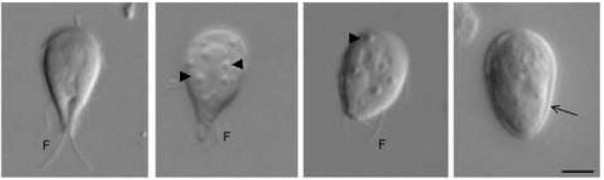
\includegraphics[width=1\textwidth]{./image/Giardia/Enquistamiento.jpg}
      \caption{Enquistamiento de \textit{Giardia Lamblia}: del trofozoíto al quiste. F, flagelos. Barra: 5 $\mu m$}
      \label{fig:enquistamiento}
    \end{figure}

    Las imágenes de izquierda a derecha muestran un trofozoíto vegetativo, trofozoítos después de 21 y
    42 horas de enquistamiento y un quiste resistente al agua, respectivamente. \cite{Lauwaet2007-te}

  \subsection{Diseño experimental}
    Se establecieron tres condiciones experimentales con el objetivo de evaluar el efecto de las
    variables asociadas al lanzamiento sobre el crecimiento y viabilidad de las muestras biológicas.
    Las condiciones diseñadas son las siguientes:
 
    \begin{itemize}
      \item \textbf{Condición de vuelo (CubeSat):} las muestras serán enviadas a bordo del CubeSat y sometidas a
        diferentes temperaturas: $10\Celsius$, $37\Celsius$ (considerada óptima para el crecimiento) y $55\Celsius$. Por
        cada zona de temperatura regulada, habrá dos muestras de 2ml cada una.

        Todas las capsulas estarán posicionadas con una inclinación de 45º con respecto al eje horizontal, condición
        necesaria para favorecer la adherencia del parásito al medio de cultivo. Se busca analizar el impacto combinado
        de la micro gravedad, las variaciones de presión, aceleraciones y la exposición térmica.

      \item \textbf{Condición control terrestre (estación terrestre):} se replicará en tierra el mismo diseño
        experimental térmico y la misma orientación espacial de las capsulas que en el CubeSat. No obstante, las
        muestras permanecerán en un entorno terrestre controlado, sin estar expuestas a los factores propios del vuelo.
        Esta condición permitirá distinguir los efectos del lanzamiento de aquellos debidos a la condición térmica
        aplicada.

      \item \textbf{Condición control optima (laboratorio):} se cultivará una muestra en condiciones optimas conocidas
        para el organismo en estudio: temperatura constante de $37\Celsius$, capsula inclinada a 45º y en ausencia de
        movimiento. Esta condición constituye el control biológico para el experimento y servirá como referencia para
        evaluar posibles desviaciones en las demás muestras.

        En todos los casos, se mantendrán constantes el tipo de recipiente utilizado, el medio de cultivo y la cantidad
        inicial de trofozoítos inoculados por capsula. Asimismo, las muestras de las primeras dos condiciones serán
        sometidas al mismo proceso de traslado previo al inicio del experimento, con el fin de asegurar homogeneidad en
        las condiciones iniciales.
    \end{itemize}

   \subsection{Procedimientos previos al lanzamiento}
   \label{sec:procedimientos-prev-lanzamiento}
    Esta sección describe los procedimientos necesarios para el cultivo y traslado de las muestras biológicas utilizadas
    en el experimento, manteniendo condiciones que aseguren su viabilidad y reproducibilidad.
 
    \subsubsection{Cultivo}
    Para cultivarlo axenicamente se utiliza medio TYI-S-33 (pH 7) suplementado con 10\% de suero
    bovino adulto y 5\% de bilis bovina (medio completo de crecimiento). Los tubos se colocaron en gradillas orientadas
    con una inclinación de aproximadamente $45\degree$, dentro de una estufa de cultivo a $37 \Celsius$.

    Luego de una hora, se comienza a observar la adhesión de los trofozoítos a las paredes del tubo a través de su disco
    ventral. De esta manera, se reproduce un entorno similar al que se encuentra in vivo, permitiendo la división de los
    trofozoítos. A las 48 horas se obtiene una monocapa de trofozoítos en etapa de crecimiento. La inclinación de las
    gradillas favorece una mayor superficie de adhesión sobre las paredes del tubo.

    \subsubsection{Traslado}
    En el día de lanzamiento, se buscarán las muestras previamente cultivadas y serán almacenadas en un lugar seguro
    en el que puedan ser transportadas bajo condiciones óptimas. Estas condiciones consisten en mantener las muestras a $37\Celsius$ y con una inclinación de
    $45\degree$. Para ello, se prevé diseñar un dispositivo de transporte con control de temperatura, regulado a
    aproximadamente $4\Celsius$, temperatura a la cual las muestras biológicas entran en un estado de inhibición metabólica
    reversible. El tiempo de traslado puede extenderse hasta las 48 horas desde la finalización del cultivo sin que esto afecte
    significativamente las condiciones de crecimiento del parásito.

  \subsection{Ensayos luego del lanzamiento}
  \label{sec:procedimientos-ensayo}
   Los ensayos se llevarán a cabo posteriormente al lanzamiento, y estarán a cargo de personal capacitado del laboratorio
   de microbiología. El objetivo es evaluar si las condiciones a las que fueron sometidas las muestras afectaron su viabilidad
   y determinar si los factores de estrés desencadenaron mecanismos clásicos de adaptación en Giardia Lamblia, tales como
   enquistamiento, apoptosis u otros procesos relacionados.
   
   Para ello, los trofozoítos serán cultivados en condiciones de anaerobiosis a 37 °C en medio TYI-S-33 (pH 7) suplementado con
   un 10\% de suero bovino adulto y un 5\% de bilis bovina (medio completo de crecimiento). La viabilidad celular se determinará
   mediante tinción con trypan blue (colorante para células no viables), utilizando la misma cantidad de trofozoítos para cada
   una de las tres condiciones experimentales previamente descritas (CubeSat, control terrestre y control óptimo en laboratorio),
   alojados en recipientes idénticos (cápsulas).

   Para el análisis de la expresión génica asociada a la respuesta al estrés, al finalizar el experimento se extraerá ARN
   (ácido ribonucleico) de cada muestra, se sintetizará ADNc (cDNA) y se realizará una cuantificación por PCR en tiempo real
   (qPCw) de genes relacionados con el estrés, como HSP70 (proteínas de choque térmico) y oxidorreductasas, empleando GDH
   como gen constitutivo de referencia. Se evaluarán cambios en la expresión respecto al cultivo control en condiciones óptimas de
   laboratorio.

   Adicionalmente, para analizar el proceso de enquistamiento , se efectuarán ensayos de inmunofluorescencia y
   observaciones mediante microscopía de fluorescencia, buscando identificar vesículas específicas de enquistamiento
   como indicadores adicionales de estrés celular.
  
  \section{Descripción del CubeSat}
  En esta sección se presenta una descripción técnica del CubeSat diseñado para llevar a cabo las misiones planteadas
  previamente. Se detallará cómo se planea abordar la implementación de los objetivos definidos, a través de la
  integración de subsistemas electrónicos, mecánicos y de software.

  Se incluyen diagramas de bloques que representan la arquitectura general del sistema y la interacción entre los
  distintos subsistemas, tales como adquisición de datos, almacenamiento, alimentación eléctrica y control de
  sensores.  Asimismo, se describen las herramientas de cálculo y simulación empleadas durante las etapas de diseño y
  verificación preliminar.

  También se presentan estimaciones iniciales de los presupuestos de masa, consumo de potencia y volumen de datos, los
  cuáles resultan fundamentales para validar la viabilidad del sistema dentro de las restricciones impuestas por la
  competencia.

  El desarrollo de esta sección tiene por objetivo demostrar la coherencia técnica entre los requerimientos de misión
  y el diseño propuesto, así como documentar las decisiones adoptadas durante el proceso de ingeniera del CubeSat.

  \subsection{General}
    En la Figura \ref{fig:sistema_general} se presenta el diagrama en bloques del sistema general desarrollado para él
    proyecto. El sistema general permite integrar la misión principal, enfocada en la recolección de parámetros
    ambientales, con una misión secundaria orientada al control y documentación de las condiciones de las muestras
    transportadas.

    \begin{figure}[H]
      \centering
      \resizebox{\textwidth}{!}{
      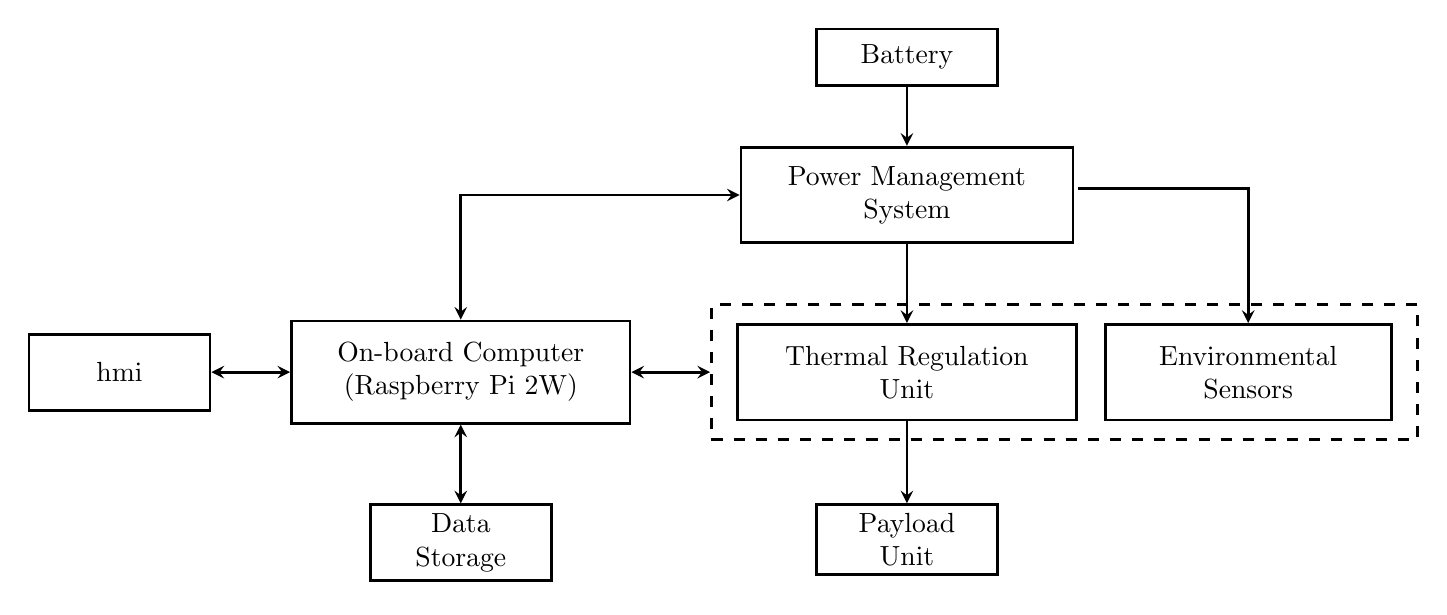
\begin{tikzpicture}
        % Paths, nodes and wires:
        \node[shape=rectangle, draw, line width=1pt, dash pattern={on 4pt off 4pt}, inner sep=0, minimum width=8.965cm, minimum height=1.715cm] at (11.833, 1.333){};
        \node[shape=rectangle, draw, line width=1pt, inner sep=0, minimum width=4.298cm, minimum height=1.215cm] at (9.833, 1.333){} node [anchor=center, align=center, text width=3.91cm, inner sep=5.5pt] at (9.833, 1.333){Thermal Regulation\\Unit};
        \node[shape=rectangle, draw, line width=1pt, inner sep=0, minimum width=3.631cm, minimum height=1.215cm] at (14.167, 1.333){} node [anchor=center, align=center, text width=3.243cm, inner sep=5.5pt] at (14.167, 1.333){Environmental Sensors};
        \node[shape=rectangle, draw, line width=1pt, inner sep=0, minimum width=2.298cm, minimum height=0.881cm] at (9.833, -0.792){} node [anchor=center, align=center, text width=1.91cm, inner sep=5.5pt] at (9.833, -0.792){Payload Unit};
        \node[shape=rectangle, draw, line width=1pt, inner sep=0, minimum width=2.298cm, minimum height=0.965cm] at (4.167, -0.833){} node [anchor=center, align=center, text width=1.91cm, inner sep=5.5pt] at (4.167, -0.833){Data Storage};
        \node[shape=rectangle, draw, line width=1pt, inner sep=0, minimum width=2.298cm, minimum height=0.715cm] at (9.833, 5.333){} node [anchor=center, align=center, text width=1.91cm, inner sep=5.5pt] at (9.833, 5.333){Battery};
        \node[shape=rectangle, draw, line width=1pt, inner sep=0, minimum width=4.298cm, minimum height=1.298cm] at (4.167, 1.333){} node [anchor=center, align=center, text width=3.91cm, inner sep=5.5pt] at (4.167, 1.333){On-board Computer\\(Raspberry Pi 2W)};
        \node[shape=rectangle, draw, line width=1pt, inner sep=0, minimum width=4.215cm, minimum height=1.215cm] at (9.833, 3.583){} node [anchor=center, align=center, text width=3.827cm, inner sep=5.5pt] at (9.833, 3.583){Power Management\\System};
        \draw[stealth-stealth, line width=1pt] (4.167, 2) |- (7.708, 3.583);
        \draw[-stealth, line width=1pt] (12, 3.667) -| (14.167, 1.958);
        \draw[stealth-, line width=1pt] (9.833, 4.208) -- (9.833, 4.958);
        \draw[stealth-, line width=1pt] (9.833, 1.958) -- (9.833, 2.958);
        \draw[stealth-stealth, line width=1pt] (4.167, 0.667) -- (4.167, -0.333);
        \node[shape=rectangle, draw, line width=1pt, inner sep=0, minimum width=2.298cm, minimum height=0.965cm] at (-0.167, 1.333){} node [anchor=center, align=center, text width=1.91cm, inner sep=5.5pt] at (-0.167, 1.333){\acrshort{hmi}};
        \draw[stealth-, line width=1pt] (9.833, -0.333) |- (9.833, 0.708);
        \draw[stealth-stealth, line width=1pt] (7.333, 1.333) -- (6.333, 1.333);
        \draw[stealth-stealth, line width=1pt] (1, 1.333) -- (2, 1.333);
      \end{tikzpicture}
      }
      \caption{Diagrama en bloques del sistema general}
      \label{fig:sistema_general}
    \end{figure}

  \subsection{Descripción de Subsistemas}
    A continuación, se describe la función de cada bloque y su interacción dentro del sistema:

  \subsubsection{Battery}
    Se emplearán cinco celdas de iones de litio (Li-Ion) con una tensión nominal de 3.6V y
    una capacidad individual de 3350mAh. Estas se conectarán todas en serie. Esta configuración proporciona una
    tensión total nominal de 19V a la misma capacidad nominal de las celdas individuales. Esta batería tiene
    aproximadamente 63.65Wh de energía, adecuada para satisfacer los requerimientos energéticos del CubeSat durante
    su operación.

  \subsubsection{Power Managment System (\acrshort{pms})}
    Es el subsistema responsable de administrar de forma segura y eficiente la energía
    proveniente de las baterías o de una fuente externa. Su función principal es distribuir la energía eléctrica a
    los distintos subsistemas del CubeSat, garantizando condiciones adecuadas de operación, mediante el monitoreo,
    la protección y la regulación.  Específicamente, las funciones del \acrshort{pms} son:
    \begin{itemize}
      \item Proteger contra cortocircuitos o sobrecarga de corriente,
      \item Permite medir parámetros eléctricos (como
        tensión y corriente) y gestionar el encendido y apagado selectivo de distintos rieles de alimentación, lo que
        contribuye a una mejor eficiencia energética y diagnóstico en vuelo, 
      \item Generar y estabilizar distintos niveles
          de tensión requeridos por los subsistemas del CubeSat, como 3.3V para sensores, 5V para la \acrshort{obc}
           y 12V para cargas específicas.
    \end{itemize}

    Con la finalidad de disminuir la carga en las baterías, se suministrará energía al \acrshort{pms} por medio de
    una fuente de alimentación externa durante la fase inicial de regulación de temperatura, ya que este es momento
    donde los elementos reguladores demandan mayor cantidad de energía.  Al llegar a las temperaturas deseadas,
    la demanda de energía es mucho menor, posibilitando la desconexión de la fuente externa sin perjudicar la
    autonomía del CubeSat.

    En definitiva, el \acrshort{pms} asegura que los requerimientos energéticos del CubeSat sean satisfechos de
    manera controlada, segura y adaptable durante toda la misión.

    \begin{figure}[H]
      \centering
      \resizebox{0.8\textwidth}{!}{
      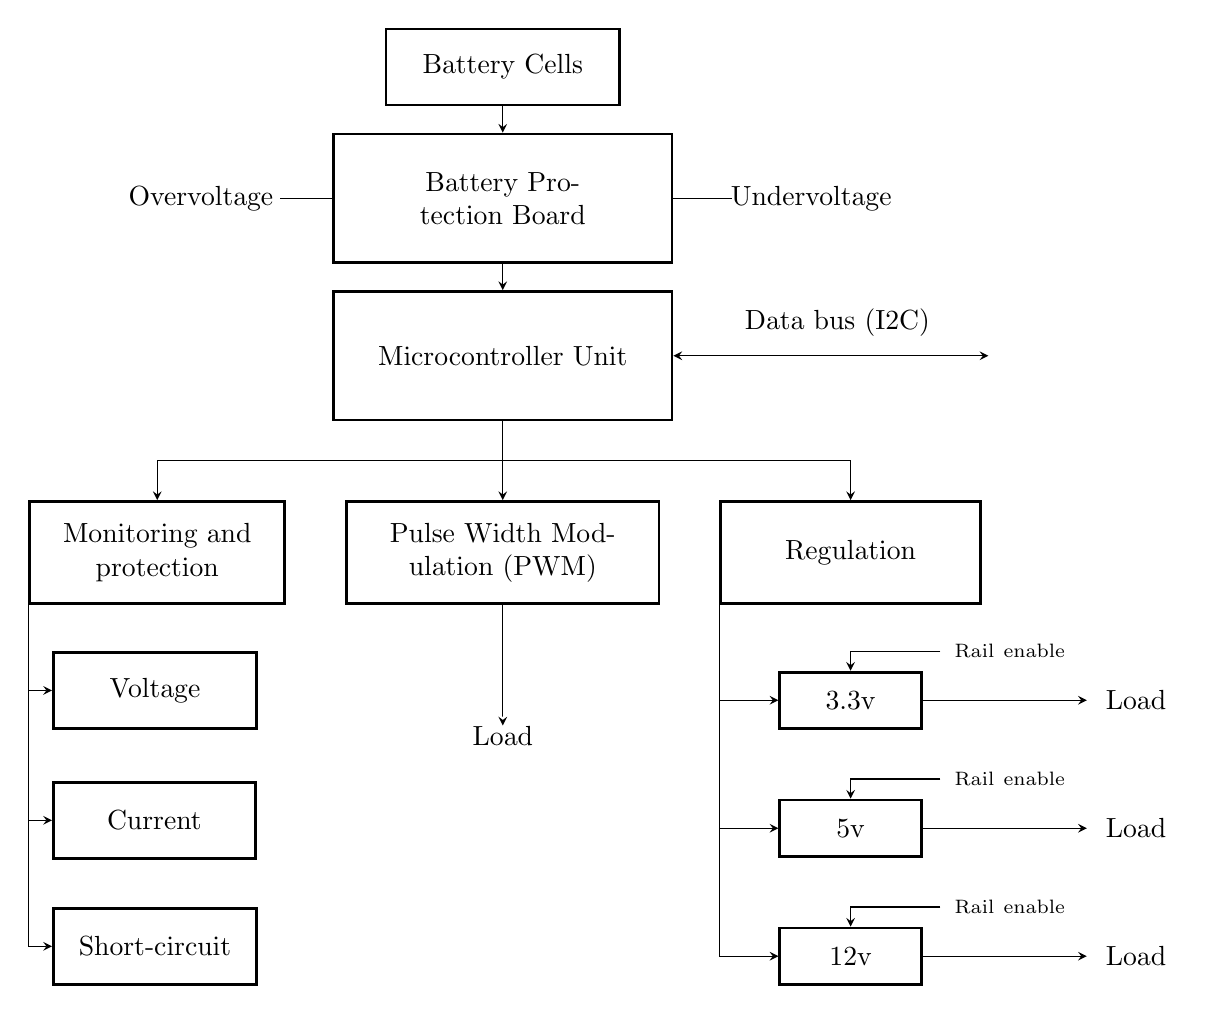
\begin{tikzpicture}
          % Paths, nodes and wires:
          \node[shape=rectangle, draw, line width=1pt, inner sep=0, minimum width=2.965cm, minimum height=0.965cm] at (8.5, 11.5){} node [anchor=center, align=center, text width=2.577cm, inner sep=5.5pt] at (8.5, 11.5){Battery Cells};
          \node[shape=rectangle, draw, line width=1pt, inner sep=0, minimum width=4.298cm, minimum height=1.631cm] at (8.5, 7.833){} node [anchor=center, align=center, text width=3.91cm, inner sep=5.5pt] at (8.5, 7.833){Microcontroller Unit\\};
          \node[shape=rectangle, draw, line width=1pt, inner sep=0, minimum width=4.298cm, minimum height=1.631cm] at (8.5, 9.833){} node [anchor=center, align=center, text width=3.91cm, inner sep=5.5pt] at (8.5, 9.833){Battery Protection Board};
          \node[shape=rectangle, inner sep=0, minimum width=2.5cm, minimum height=1cm] at (4.667, 9.833){} node [anchor=center, align=center, text width=2.147cm, inner sep=5pt] at (4.667, 9.833){Overvoltage};
          \node[shape=rectangle, draw, line width=1pt, inner sep=0, minimum width=3.24cm, minimum height=1.298cm] at (4.112, 5.333){} node [anchor=center, align=center, text width=2.852cm, inner sep=5.5pt] at (4.112, 5.333){Monitoring and\\protection\\};
          \node[shape=rectangle, draw, line width=1pt, inner sep=0, minimum width=1.798cm, minimum height=0.715cm] at (12.917, 3.458){} node [anchor=center, align=center, text width=1.41cm, inner sep=5.5pt] at (12.917, 3.458){3.3v};
          \node[shape=rectangle, draw, line width=1pt, inner sep=0, minimum width=3.298cm, minimum height=1.298cm] at (12.917, 5.333){} node [anchor=center, align=center, text width=2.91cm, inner sep=5.5pt] at (12.917, 5.333){Regulation\\};
          \node[shape=rectangle, draw, line width=1pt, inner sep=0, minimum width=2.581cm, minimum height=0.965cm] at (4.083, 0.333){} node [anchor=center, align=center, text width=2.193cm, inner sep=5.5pt] at (4.083, 0.333){Short-circuit};
          \draw[-stealth] (8.5, 9) -| (8.5, 8.667);
          \draw[-stealth] (8.5, 11) -| (8.5, 10.667);
          \draw[-stealth] (13.833, 3.458) -- (15.917, 3.458);
          \draw[stealth-stealth] (10.667, 7.833) -- (14.667, 7.833);
          \node[shape=rectangle, draw, line width=1pt, inner sep=0, minimum width=2.581cm, minimum height=0.965cm] at (4.083, 3.583){} node [anchor=center, align=center, text width=2.193cm, inner sep=5.5pt] at (4.083, 3.583){Voltage};
          \node[shape=rectangle, inner sep=0, minimum width=3.333cm, minimum height=0.667cm] at (12.75, 8.25){} node [anchor=center, align=center, text width=2.981cm, inner sep=5pt] at (12.75, 8.25){Data bus (I2C)};
          \node[shape=rectangle, inner sep=0, minimum width=2.5cm, minimum height=1cm] at (12.417, 9.833){} node [anchor=center, align=center, text width=2.147cm, inner sep=5pt] at (12.417, 9.833){Undervoltage};
          \draw (6.333, 9.833) -| (5.667, 9.833);
          \draw (10.667, 9.833) -- (11.417, 9.833);
          \node[shape=rectangle, draw, line width=1pt, inner sep=0, minimum width=2.565cm, minimum height=0.965cm] at (4.075, 1.933){} node [anchor=center, align=center, text width=2.177cm, inner sep=5.5pt] at (4.075, 1.933){Current};
          \node[shape=rectangle, inner sep=0, minimum width=2.063cm, minimum height=0.5cm] at (15.087, 4.083){} node [anchor=west, align=left, text width=1.71cm, inner sep=5pt] at (14.056, 4.083){\scriptsize Rail enable};
          \draw[-stealth] (14.056, 4.083) -| (12.917, 3.833);
          \node[shape=rectangle, draw, line width=1pt, inner sep=0, minimum width=1.798cm, minimum height=0.715cm] at (12.917, 1.833){} node [anchor=center, align=center, text width=1.41cm, inner sep=5.5pt] at (12.917, 1.833){5v};
          \draw[-stealth] (13.833, 1.833) -- (15.917, 1.833);
          \node[shape=rectangle, inner sep=0, minimum width=2.063cm, minimum height=0.5cm] at (15.087, 2.458){} node [anchor=west, align=left, text width=1.71cm, inner sep=5pt] at (14.056, 2.458){\scriptsize Rail enable};
          \draw[-stealth] (14.056, 2.458) -| (12.917, 2.208);
          \node[shape=rectangle, draw, line width=1pt, inner sep=0, minimum width=1.798cm, minimum height=0.715cm] at (12.917, 0.208){} node [anchor=center, align=center, text width=1.41cm, inner sep=5.5pt] at (12.917, 0.208){12v};
          \draw[-stealth] (13.833, 0.208) -- (15.917, 0.208);
          \node[shape=rectangle, inner sep=0, minimum width=2.063cm, minimum height=0.5cm] at (15.087, 0.833){} node [anchor=west, align=left, text width=1.71cm, inner sep=5pt] at (14.056, 0.833){\scriptsize Rail enable};
          \draw[-stealth] (14.056, 0.833) -| (12.917, 0.583);
          \draw[-stealth] (11.25, 4.667) |- (12, 0.208);
          \draw[stealth-] (12, 1.833) -| (11.247, 1.829);
          \draw[stealth-] (12, 3.458) -| (11.252, 3.461);
          \draw[-stealth] (2.475, 4.667) |- (2.775, 0.333);
          \draw[stealth-] (2.775, 3.583) -| (2.473, 3.591);
          \draw[stealth-] (2.775, 1.933) -| (2.474, 1.94);
          \node[shape=rectangle, draw, line width=1pt, inner sep=0, minimum width=3.965cm, minimum height=1.298cm] at (8.5, 5.333){} node [anchor=center, align=center, text width=3.577cm, inner sep=5.5pt] at (8.5, 5.333){Pulse Width Modulation (PWM)\\};
          \node[shape=rectangle, inner sep=0, minimum width=1.25cm, minimum height=0.5cm] at (8.5, 3){} node [anchor=center, align=center, text width=0.897cm, inner sep=5pt] at (8.5, 3){Load};
          \draw[stealth reversed-] (8.5, 3.25) -| (8.5, 4.667);
          \node[shape=rectangle, inner sep=0, minimum width=1.25cm, minimum height=0.5cm] at (16.542, 3.458){} node [anchor=center, align=center, text width=0.897cm, inner sep=5pt] at (16.542, 3.458){Load};
          \node[shape=rectangle, inner sep=0, minimum width=1.25cm, minimum height=0.5cm] at (16.542, 1.833){} node [anchor=center, align=center, text width=0.897cm, inner sep=5pt] at (16.542, 1.833){Load};
          \node[shape=rectangle, inner sep=0, minimum width=1.25cm, minimum height=0.5cm] at (16.542, 0.208){} node [anchor=center, align=center, text width=0.897cm, inner sep=5pt] at (16.542, 0.208){Load};
          \draw[-stealth] (8.5, 7) -| (8.5, 6);
          \draw[stealth-] (4.112, 6) |- (8.5, 6.5);
          \draw[stealth-] (12.917, 6) |- (8.5, 6.5);
      \end{tikzpicture}
      }
      \caption{Diagrama en bloques del \acrshort{pms}.}
      \label{fig:sistema_pms}
    \end{figure}

  \subsubsection{On-board Computer (\acrshort{obc})}
    Tiene como función principal la gestión autónoma de la misión
    durante todo el vuelo. Esta unidad está basada en una Raspberry Pi Zero 2 W, equipada con el sistema operativo
    Raspberry Pi OS Lite, una versión optimizada sin entorno gráfico. Esta configuración fue seleccionada por su
    bajo consumo energético, reducido tamaño y alta estabilidad operativa.

    El propósito fundamental del \acrshort{obc} es leer y almacenar el registro de los sensores, tales como
    aceleración, orientación, presión atmosférica y temperatura ambiente. Estas mediciones son gestionadas por un
    programa que se ejecuta de manera automática, y almacenadas de forma estructurada, facilitando su posterior
    lectura y procesamiento. También es responsable del control de subsistemas clave, como la \acrfull{tru} , utilizado
    para la misión secundaria, en conjunto con el \acrfull{pms}.

    Una vez finalizado el vuelo, los archivos generados estarán disponibles al usuario usando el \acrshort{hmi},
    permitiendo su análisis y visualización sin necesidad de equipo especializado. Esta separación entre adquisición
    y procesamiento permite una asignación eficiente de recursos, manteniendo al \acrshort{obc} centrado
    exclusivamente en tareas críticas durante la misión.

    \begin{figure}[H]
      \centering
      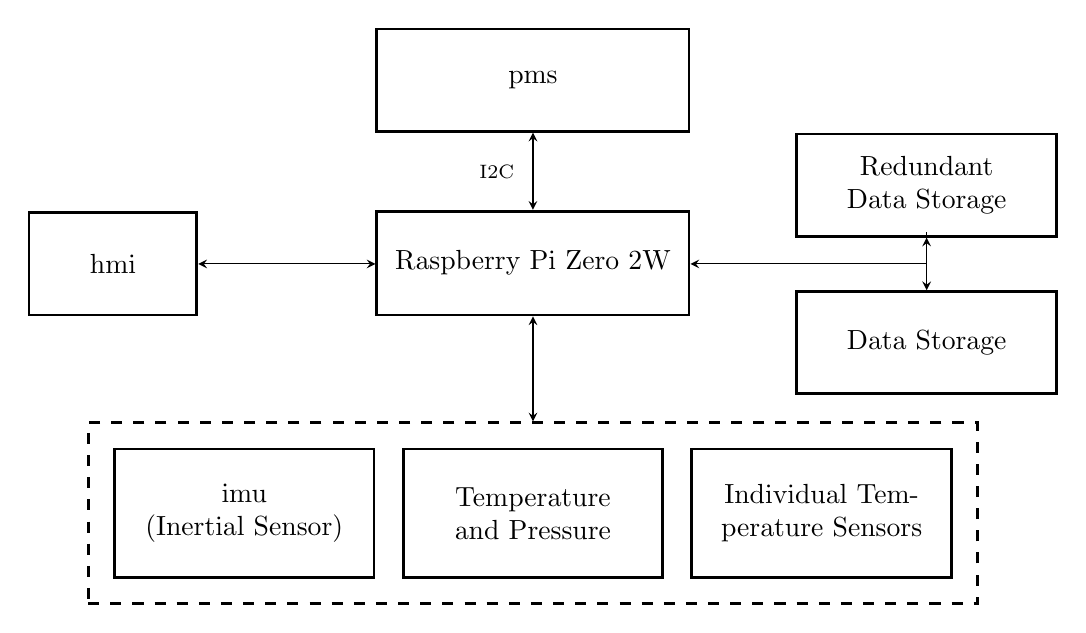
\begin{tikzpicture}
        % Paths, nodes and wires:
        \node[shape=rectangle, draw, line width=1pt, inner sep=0, minimum width=3.965cm, minimum height=1.319cm] at (9.667, 3.344){} node [anchor=center, align=center, text width=3.577cm, inner sep=5.5pt] at (9.667, 3.344){Raspberry Pi Zero 2W};
        \node[shape=rectangle, draw, line width=1pt, inner sep=0, minimum width=3.298cm, minimum height=1.631cm] at (6, 0.167){} node [anchor=center, align=center, text width=2.91cm, inner sep=5.5pt] at (6, 0.167){\acrshort{imu}\\(Inertial Sensor)};
        \node[shape=rectangle, draw, line width=1pt, inner sep=0, minimum width=3.298cm, minimum height=1.298cm] at (14.667, 4.333){} node [anchor=center, align=center, text width=2.91cm, inner sep=5.5pt] at (14.667, 4.333){Redundant Data Storage};
        \node[shape=rectangle, draw, line width=1pt, inner sep=0, minimum width=2.131cm, minimum height=1.298cm] at (4.333, 3.333){} node [anchor=center, align=center, text width=1.743cm, inner sep=5.5pt] at (4.333, 3.333){\acrshort{hmi}};
        \node[shape=rectangle, draw, line width=1pt, inner sep=0, minimum width=3.298cm, minimum height=1.631cm] at (9.667, 0.167){} node [anchor=center, align=center, text width=2.91cm, inner sep=5.5pt] at (9.667, 0.167){Temperature and Pressure};
        \node[shape=rectangle, draw, line width=1pt, inner sep=0, minimum width=3.298cm, minimum height=1.631cm] at (13.333, 0.167){} node [anchor=center, align=center, text width=2.91cm, inner sep=5.5pt] at (13.333, 0.167){Individual Temperature Sensors};
        \node[shape=rectangle, draw, line width=1pt, dash pattern={on 4pt off 4pt}, inner sep=0, minimum width=11.298cm, minimum height=2.298cm] at (9.667, 0.167){};
        \node[shape=rectangle, draw, line width=1pt, inner sep=0, minimum width=3.298cm, minimum height=1.298cm] at (14.667, 2.333){} node [anchor=center, align=center, text width=2.91cm, inner sep=5.5pt] at (14.667, 2.333){Data Storage};
        \node[shape=rectangle, draw, line width=1pt, inner sep=0, minimum width=3.965cm, minimum height=1.298cm] at (9.667, 5.667){} node [anchor=center, align=center, text width=3.577cm, inner sep=5.5pt] at (9.667, 5.667){\acrshort{pms}};
        \node[shape=rectangle, inner sep=0, minimum width=0.917cm, minimum height=0.667cm] at (9.208, 4.5){} node [anchor=center, align=center, text width=0.564cm, inner sep=5pt] at (9.208, 4.5){\scriptsize I2C};
        \draw[stealth-stealth] (7.667, 3.333) -- (5.417, 3.333);
        \draw[stealth-stealth] (9.667, 4.021) -- (9.667, 5);
        \draw[stealth-stealth] (9.667, 2.667) -- (9.667, 1.333);
        \draw[stealth-] (11.667, 3.333) -- (14.667, 3.333);
        \draw[stealth-stealth] (14.667, 3.667) -| (14.667, 3);
      \end{tikzpicture}
      \caption{Diagrama en bloques del \acrshort{obc}.}
      \label{fig:sistema_obc}
    \end{figure}

   En el diagrama ~\ref{fig:filesystem} se presenta la estructura del sistema de archivos diseñada para la misión.
   Cada dato capturado por los sensores es leído por la \acrshort{obc}, que se encarga de almacenar dicho dato en un archivo
   específico. Junto a este archivo, se crea un segundo archivo con el mismo nombre seguido del sufijo "\_timestamp",
   donde se guardará la marca de tiempo en que se tomó la medición.
   
   Estos archivos son de texto plano codificado en ASCII, y estarán continuamente sobreescribiéndose, conteniendo en
   todo momento únicamente el dato o timestamp más reciente. Paralelamente, un programa adicional monitorea estos
   archivos en tiempo real, leyendo los datos y sus respectivos timestamps a medida que se actualizan. Además, agrupará
   la información y la almacenará en un archivo CSV, dentro del directorio \textit{data/}, combinando los valores con
   sus timestamps correspondientes.

   El archivo CSV resultante cumple dos funciones clave:
    \begin{itemize}
        \item Permite que el \acrshort{hmi} lea y muestre los datos en tiempo real para supervisión.
        \item Facilita el postprocesamiento, donde los datos serán graficados, permitiendo su análisis visual
        para extraer conclusiones sobre el comportamiento del sistema y la misión.
    \end{itemize}

    \begin{figure}[H]
        \centering
        \resizebox{0.85\textwidth}{!}{%
        \begin{minipage}[t]{0.32\textwidth}
        \vspace{0pt}
        \begin{forest}
          for tree={
            font=\ttfamily,
            grow'=0,
            child anchor=west,
            parent anchor=south,
            anchor=west,
            calign=first,
            inner xsep=7pt,
            before typesetting nodes={
              if n=1
                {insert before={[,phantom]}}
                {}
            },
            fit=band,
            before computing xy={l=15pt},
          }
        [lambda/, folder node
          [modules/, folder node
            [pms/, folder node
              [bat/, folder node
                [vbat1, file node]
                [vbat2, file node]
                [vbat3, file node]
                [vbat4, file node]
                [vbat5, file node]
                [temp, file node]
              ]
            ]
            [sources/, folder node
               [vbat, file node]
               [rail\_3v, file node]
               [rail\_3v\_en, file node]
               [rail\_5v, file node]
               [rail\_5v\_en, file node]
               [rail\_12v, file node]
               [rail\_12v\_en, file node]
            ]
          ]
        ]
        \end{forest}
        \end{minipage}%
        \hfill
        \begin{minipage}[t]{0.32\textwidth}
        \vspace{0pt}
        \begin{forest}
          for tree={
            font=\ttfamily,
            grow'=0,
            child anchor=west,
            parent anchor=south,
            anchor=west,
            calign=first,
            inner xsep=7pt,
            before typesetting nodes={
              if n=1
                {insert before={[,phantom]}}
                {}
            },
            fit=band,
            before computing xy={l=15pt},
          }
        [lambda/, folder node
            [modules/, folder node
               [obc/, folder node
                 [gyro/, folder node
                    [x\_axis, file node]
                    [y\_axis, file node]
                    [z\_axis, file node]
                 ]
                 [accel/, folder node
                    [x\_axis, file node]
                    [y\_axis, file node]
                    [z\_axis, file node]
                 ]
                 [magn/, folder node
                    [x\_axis, file node]
                    [y\_axis, file node]
                    [z\_axis, file node]
                 ]
                 [temp/, folder node
                    [bmp, file node]
                    [mpu, file node]
                 ]
                 [press, file node]
                 [mode, file node]
               ]
            ]
        ]
        \end{forest}
        \end{minipage}%
        \hfill
        \begin{minipage}[t]{0.32\textwidth}
        \vspace{0pt}
        \begin{forest}
          for tree={
            font=\ttfamily,
            grow'=0,
            child anchor=west,
            parent anchor=south,
            anchor=west,
            calign=first,
            inner xsep=7pt,
            before typesetting nodes={
              if n=1
                {insert before={[,phantom]}}
                {}
            },
            fit=band,
            before computing xy={l=15pt},
          }
        [lambda/, folder node
            [modules, folder node
              [tru/, folder node
                [pwm/, folder node
                  [tu1, file node]
                  [tu2, file node]
                  [tu3, file node]
                 ]
                [temp/, folder node
                  [tu1, file node]
                  [tu2, file node]
                  [tu3, file node]
                 ]
              ]
            ]
          [data/, folder node
            [log.txt, file node]
            [mission.csv, file node]
          ]
        ]
        \end{forest}
        \end{minipage}%
        }
    \caption{Sistema de archivos para la misión.}
    \label{fig:filesystem}
    \end{figure} 

    \subsubsection{Human-Machine Interface \acrshort{hmi}}
      La principal forma de interacción entre el usuario y él
      CubeSat es mediante la \acrshort{hmi}. Esta interfaz es un compuesto entre físico y virtual. 

      La parte física del \acrshort{hmi} involucra un conector que está expuesto al exterior, el cual dependiendo de que
      conector o "llave" se le conecte, altera el funcionamiento del CubeSat. Esto permite una gestión eficiente de los
      recursos, especialmente en lo que respecta al consumo de potencia y la preparación del CubeSat para eventos
      críticos de la misión, mediante la adaptación de su funcionamiento según la etapa de la misión. Se han definido
      los siguientes modos de operación:
      \begin{itemize}
        \item \textbf{Apagado:} En este modo la línea principal de alimentación se desconecta mediante un MOSFET,
          asegurando el apagado completo del CubeSat.
        \item \textbf{Pre Lanzamiento:} Inicializa los subsistemas y corrobora el correcto funcionamiento. Permite la
          conexión a la interfaz web mediante WiFi. Una vez inicializados los subsistemas y realizadas las
          verificaciones pertinentes, el sistema se pone en modo de reposo.
        \item \textbf{Reposo:} Las unidades de procesamiento principal (RPI en la OBC y Arduino Nano en el PMS) entran
          en modos de bajo consumo de potencia (idle, stand-by, deep sleep, etc.). Se disminuye la frecuencia de lectura
          de ciertos sensores. Si el modo anterior fue el de \textit{pre lanzamiento} el subsistema \acrshort{tru} sé
          mantiene activo.
        \item \textbf{Lanzamiento:} Este modo se activa cuando el conector externo está ausente, funcionando como un mecanismo de
            "Remove Before Flight". En esta condición, el CubeSat ejecuta únicamente las rutinas críticas necesarias para garantizar
             el cumplimiento de la misión, evitando operaciones no esenciales durante la fase de lanzamiento.
        \item \textbf{Recuperación de datos:} Rehabilita la comunicación con la estación terrestre permitiendo la
          descarga de datos para su posterior procesamiento y análisis.
        \item \textbf{Prueba:} Este modo será utilizado durante le desarrollo del CubeSat permitiendo acceso
          administrativo al sistema.
      \end{itemize}

      \begin{wrapfigure}{L}{0.3\textwidth}
        \centering
        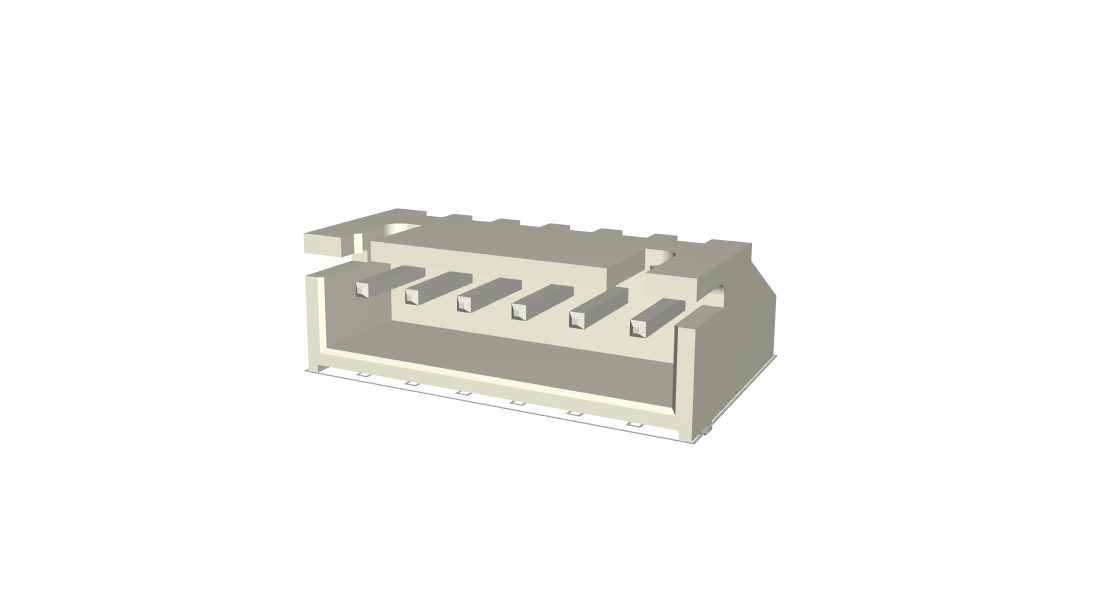
\includegraphics[width=0.9\linewidth]{image/conector/conector-jst.png}
        \caption{Conector JST HX de 6 pines macho.}
        \label{fig:conector-jst}
      \end{wrapfigure}
      El conector utilizado es un JST HX de 6 pines (macho en la \acrshort{obc} y hembra para el usuario) (fig.
      ~\ref{fig:conector-jst}), de los cuales 3 pines son leídos por la Raspberry Pi. Esos pines están configurados con
      resistencias pull-up. Esto significa que, en ausencia de conexión externa, dichas entradas leen un nivel lógico
      alto (1). Las diferentes "llaves" conectarán los pines leídos por la Raspberry Pi en diferentes puntos, los cuales
      son los que determinan el modo de operación. En la figura \ref{fig:seleccion_modos} se puede ver una
      representación de la parte física del \acrshort{hmi}.


      \begin{figure}[H]
        \centering
        \resizebox{0.9\textwidth}{!}{%
         \begin{tikzpicture}
            \node[shape=rectangle, minimum width=2.5cm, minimum height=0.75cm] at (24.406, 5.625){} node[anchor=north, align=center, text width=2.147cm, inner sep=5pt] at (24.406, 6){Lanzamiento};
            \node[shape=rectangle, minimum width=2.875cm, minimum height=0.75cm] at (18.5, 8.25){} node[anchor=north, align=center, text width=2.522cm, inner sep=5pt] at (18.5, 8.625){Reposo};
            \node[shape=rectangle, minimum width=2.875cm, minimum height=0.75cm] at (24.375, 8.25){} node[anchor=north, align=center, text width=2.522cm, inner sep=5pt] at (24.375, 8.625){Prueba};
            \node[shape=rectangle, minimum width=2.875cm, minimum height=0.75cm] at (12.625, 8.25){} node[anchor=north, align=center, text width=2.522cm, inner sep=5pt] at (12.625, 8.625){Apagado};
            \node[shape=rectangle, minimum width=2.875cm, minimum height=0.75cm] at (12.656, 5.625){} node[anchor=north, align=center, text width=2.522cm, inner sep=5pt] at (12.656, 6){Rec. de datos};
            \node[shape=rectangle, draw, line width=1pt, minimum width=4.465cm, minimum height=1.215cm] at (12.625, 7.25){};
            \node[shape=rectangle, draw, line width=1pt, minimum width=0.215cm, minimum height=0.215cm] at (10.75, 7.25){};
            \node[shape=rectangle, draw, line width=1pt, minimum width=0.215cm, minimum height=0.215cm] at (11.5, 7.25){};
            \node[shape=rectangle, draw, line width=1pt, minimum width=0.215cm, minimum height=0.215cm] at (12.25, 7.25){};
            \node[shape=rectangle, draw, line width=1pt, minimum width=0.215cm, minimum height=0.215cm] at (13, 7.25){};
            \node[shape=rectangle, draw, line width=1pt, minimum width=0.215cm, minimum height=0.215cm] at (13.75, 7.25){};
            \node[shape=rectangle, draw, line width=1pt, minimum width=0.215cm, minimum height=0.215cm] at (14.5, 7.25){};
            \node[shape=rectangle, minimum width=0.5cm, minimum height=0.5cm] at (10.625, 6.875){} node[anchor=north, align=center, text width=0.147cm, inner sep=5pt] at (10.625, 7.125){\tiny 1};
            \node[shape=rectangle, minimum width=0.5cm, minimum height=0.5cm] at (11.375, 6.875){} node[anchor=north, align=center, text width=0.147cm, inner sep=5pt] at (11.375, 7.125){\tiny 2};
            \node[shape=rectangle, minimum width=0.5cm, minimum height=0.5cm] at (12.125, 6.875){} node[anchor=north, align=center, text width=0.147cm, inner sep=5pt] at (12.125, 7.125){\tiny 3};
            \node[shape=rectangle, minimum width=0.5cm, minimum height=0.5cm] at (12.875, 6.875){} node[anchor=north, align=center, text width=0.147cm, inner sep=5pt] at (12.875, 7.125){\tiny 4};
            \node[shape=rectangle, minimum width=0.5cm, minimum height=0.5cm] at (13.625, 6.875){} node[anchor=north, align=center, text width=0.147cm, inner sep=5pt] at (13.625, 7.125){\tiny 5};
            \node[shape=rectangle, minimum width=0.5cm, minimum height=0.5cm] at (14.375, 6.875){} node[anchor=north, align=center, text width=0.147cm, inner sep=5pt] at (14.375, 7.125){\tiny 6};
            \node[shape=rectangle, draw, line width=1pt, minimum width=4.465cm, minimum height=1.215cm] at (24.375, 7.25){};
            \node[shape=rectangle, draw, line width=1pt, minimum width=0.215cm, minimum height=0.215cm] at (22.5, 7.25){};
            \node[shape=rectangle, draw, line width=1pt, minimum width=0.215cm, minimum height=0.215cm] at (23.25, 7.25){};
            \node[shape=rectangle, draw, line width=1pt, minimum width=0.215cm, minimum height=0.215cm] at (24, 7.25){};
            \node[shape=rectangle, draw, line width=1pt, minimum width=0.215cm, minimum height=0.215cm] at (24.75, 7.25){};
            \node[shape=rectangle, draw, line width=1pt, minimum width=0.215cm, minimum height=0.215cm] at (25.5, 7.25){};
            \node[shape=rectangle, draw, line width=1pt, minimum width=0.215cm, minimum height=0.215cm] at (26.25, 7.25){};
            \node[shape=rectangle, minimum width=0.5cm, minimum height=0.5cm] at (22.375, 6.875){} node[anchor=north, align=center, text width=0.147cm, inner sep=5pt] at (22.375, 7.125){\tiny 1};
            \node[shape=rectangle, minimum width=0.5cm, minimum height=0.5cm] at (23.125, 6.875){} node[anchor=north, align=center, text width=0.147cm, inner sep=5pt] at (23.125, 7.125){\tiny 2};
            \node[shape=rectangle, minimum width=0.5cm, minimum height=0.5cm] at (23.875, 6.875){} node[anchor=north, align=center, text width=0.147cm, inner sep=5pt] at (23.875, 7.125){\tiny 3};
            \node[shape=rectangle, minimum width=0.5cm, minimum height=0.5cm] at (24.625, 6.875){} node[anchor=north, align=center, text width=0.147cm, inner sep=5pt] at (24.625, 7.125){\tiny 4};
            \node[shape=rectangle, minimum width=0.5cm, minimum height=0.5cm] at (25.375, 6.875){} node[anchor=north, align=center, text width=0.147cm, inner sep=5pt] at (25.375, 7.125){\tiny 5};
            \node[shape=rectangle, minimum width=0.5cm, minimum height=0.5cm] at (26.125, 6.875){} node[anchor=north, align=center, text width=0.147cm, inner sep=5pt] at (26.125, 7.125){\tiny 6};
            \node[shape=rectangle, draw, line width=1pt, minimum width=4.465cm, minimum height=1.215cm] at (12.656, 4.625){};
            \node[shape=rectangle, draw, line width=1pt, minimum width=0.215cm, minimum height=0.215cm] at (10.781, 4.625){};
            \node[shape=rectangle, draw, line width=1pt, minimum width=0.215cm, minimum height=0.215cm] at (11.531, 4.625){};
            \node[shape=rectangle, draw, line width=1pt, minimum width=0.215cm, minimum height=0.215cm] at (12.281, 4.625){};
            \node[shape=rectangle, draw, line width=1pt, minimum width=0.215cm, minimum height=0.215cm] at (13.031, 4.625){};
            \node[shape=rectangle, draw, line width=1pt, minimum width=0.215cm, minimum height=0.215cm] at (13.781, 4.625){};
            \node[shape=rectangle, draw, line width=1pt, minimum width=0.215cm, minimum height=0.215cm] at (14.531, 4.625){};
            \node[shape=rectangle, minimum width=0.5cm, minimum height=0.5cm] at (10.656, 4.25){} node[anchor=north, align=center, text width=0.147cm, inner sep=5pt] at (10.656, 4.5){\tiny 1};
            \node[shape=rectangle, minimum width=0.5cm, minimum height=0.5cm] at (11.406, 4.25){} node[anchor=north, align=center, text width=0.147cm, inner sep=5pt] at (11.406, 4.5){\tiny 2};
            \node[shape=rectangle, minimum width=0.5cm, minimum height=0.5cm] at (12.156, 4.25){} node[anchor=north, align=center, text width=0.147cm, inner sep=5pt] at (12.156, 4.5){\tiny 3};
            \node[shape=rectangle, minimum width=0.5cm, minimum height=0.5cm] at (12.906, 4.25){} node[anchor=north, align=center, text width=0.147cm, inner sep=5pt] at (12.906, 4.5){\tiny 4};
            \node[shape=rectangle, minimum width=0.5cm, minimum height=0.5cm] at (13.656, 4.25){} node[anchor=north, align=center, text width=0.147cm, inner sep=5pt] at (13.656, 4.5){\tiny 5};
            \node[shape=rectangle, minimum width=0.5cm, minimum height=0.5cm] at (14.406, 4.25){} node[anchor=north, align=center, text width=0.147cm, inner sep=5pt] at (14.406, 4.5){\tiny 6};
            \node[shape=rectangle, draw, line width=1pt, minimum width=4.465cm, minimum height=1.215cm] at (18.5, 7.25){};
            \node[shape=rectangle, draw, line width=1pt, minimum width=0.215cm, minimum height=0.215cm] at (16.625, 7.25){};
            \node[shape=rectangle, draw, line width=1pt, minimum width=0.215cm, minimum height=0.215cm] at (17.375, 7.25){};
            \node[shape=rectangle, draw, line width=1pt, minimum width=0.215cm, minimum height=0.215cm] at (18.125, 7.25){};
            \node[shape=rectangle, draw, line width=1pt, minimum width=0.215cm, minimum height=0.215cm] at (18.875, 7.25){};
            \node[shape=rectangle, draw, line width=1pt, minimum width=0.215cm, minimum height=0.215cm] at (19.625, 7.25){};
            \node[shape=rectangle, draw, line width=1pt, minimum width=0.215cm, minimum height=0.215cm] at (20.375, 7.25){};
            \node[shape=rectangle, minimum width=0.5cm, minimum height=0.5cm] at (16.5, 6.875){} node[anchor=north, align=center, text width=0.147cm, inner sep=5pt] at (16.5, 7.125){\tiny 1};
            \node[shape=rectangle, minimum width=0.5cm, minimum height=0.5cm] at (17.25, 6.875){} node[anchor=north, align=center, text width=0.147cm, inner sep=5pt] at (17.25, 7.125){\tiny 2};
            \node[shape=rectangle, minimum width=0.5cm, minimum height=0.5cm] at (18, 6.875){} node[anchor=north, align=center, text width=0.147cm, inner sep=5pt] at (18, 7.125){\tiny 3};
            \node[shape=rectangle, minimum width=0.5cm, minimum height=0.5cm] at (18.75, 6.875){} node[anchor=north, align=center, text width=0.147cm, inner sep=5pt] at (18.75, 7.125){\tiny 4};
            \node[shape=rectangle, minimum width=0.5cm, minimum height=0.5cm] at (19.5, 6.875){} node[anchor=north, align=center, text width=0.147cm, inner sep=5pt] at (19.5, 7.125){\tiny 5};
            \node[shape=rectangle, minimum width=0.5cm, minimum height=0.5cm] at (20.25, 6.875){} node[anchor=north, align=center, text width=0.147cm, inner sep=5pt] at (20.25, 7.125){\tiny 6};
            \node[shape=rectangle, draw, line width=1pt, minimum width=4.465cm, minimum height=1.215cm] at (18.5, 4.625){};
            \node[shape=rectangle, draw, line width=1pt, minimum width=0.215cm, minimum height=0.215cm] at (16.625, 4.625){};
            \node[shape=rectangle, draw, line width=1pt, minimum width=0.215cm, minimum height=0.215cm] at (17.375, 4.625){};
            \node[shape=rectangle, draw, line width=1pt, minimum width=0.215cm, minimum height=0.215cm] at (18.125, 4.625){};
            \node[shape=rectangle, draw, line width=1pt, minimum width=0.215cm, minimum height=0.215cm] at (18.875, 4.625){};
            \node[shape=rectangle, draw, line width=1pt, minimum width=0.215cm, minimum height=0.215cm] at (19.625, 4.625){};
            \node[shape=rectangle, draw, line width=1pt, minimum width=0.215cm, minimum height=0.215cm] at (20.375, 4.625){};
            \node[shape=rectangle, minimum width=0.5cm, minimum height=0.5cm] at (16.5, 4.25){} node[anchor=north, align=center, text width=0.147cm, inner sep=5pt] at (16.5, 4.5){\tiny 1};
            \node[shape=rectangle, minimum width=0.5cm, minimum height=0.5cm] at (17.25, 4.25){} node[anchor=north, align=center, text width=0.147cm, inner sep=5pt] at (17.25, 4.5){\tiny 2};
            \node[shape=rectangle, minimum width=0.5cm, minimum height=0.5cm] at (18, 4.25){} node[anchor=north, align=center, text width=0.147cm, inner sep=5pt] at (18, 4.5){\tiny 3};
            \node[shape=rectangle, minimum width=0.5cm, minimum height=0.5cm] at (18.75, 4.25){} node[anchor=north, align=center, text width=0.147cm, inner sep=5pt] at (18.75, 4.5){\tiny 4};
            \node[shape=rectangle, minimum width=0.5cm, minimum height=0.5cm] at (19.5, 4.25){} node[anchor=north, align=center, text width=0.147cm, inner sep=5pt] at (19.5, 4.5){\tiny 5};
            \node[shape=rectangle, minimum width=0.5cm, minimum height=0.5cm] at (20.25, 4.25){} node[anchor=north, align=center, text width=0.147cm, inner sep=5pt] at (20.25, 4.5){\tiny 6};
            \node[shape=rectangle, draw, line width=1pt, minimum width=4.465cm, minimum height=1.215cm] at (24.406, 4.625){};
            \node[shape=rectangle, draw, line width=1pt, minimum width=0.215cm, minimum height=0.215cm] at (22.531, 4.625){};
            \node[shape=rectangle, draw, line width=1pt, minimum width=0.215cm, minimum height=0.215cm] at (23.281, 4.625){};
            \node[shape=rectangle, draw, line width=1pt, minimum width=0.215cm, minimum height=0.215cm] at (24.031, 4.625){};
            \node[shape=rectangle, draw, line width=1pt, minimum width=0.215cm, minimum height=0.215cm] at (24.781, 4.625){};
            \node[shape=rectangle, draw, line width=1pt, minimum width=0.215cm, minimum height=0.215cm] at (25.531, 4.625){};
            \node[shape=rectangle, draw, line width=1pt, minimum width=0.215cm, minimum height=0.215cm] at (26.281, 4.625){};
            \node[shape=rectangle, minimum width=0.5cm, minimum height=0.5cm] at (22.406, 4.25){} node[anchor=north, align=center, text width=0.147cm, inner sep=5pt] at (22.406, 4.5){\tiny 1};
            \node[shape=rectangle, minimum width=0.5cm, minimum height=0.5cm] at (23.156, 4.25){} node[anchor=north, align=center, text width=0.147cm, inner sep=5pt] at (23.156, 4.5){\tiny 2};
            \node[shape=rectangle, minimum width=0.5cm, minimum height=0.5cm] at (23.906, 4.25){} node[anchor=north, align=center, text width=0.147cm, inner sep=5pt] at (23.906, 4.5){\tiny 3};
            \node[shape=rectangle, minimum width=0.5cm, minimum height=0.5cm] at (24.656, 4.25){} node[anchor=north, align=center, text width=0.147cm, inner sep=5pt] at (24.656, 4.5){\tiny 4};
            \node[shape=rectangle, minimum width=0.5cm, minimum height=0.5cm] at (25.406, 4.25){} node[anchor=north, align=center, text width=0.147cm, inner sep=5pt] at (25.406, 4.5){\tiny 5};
            \node[shape=rectangle, minimum width=0.5cm, minimum height=0.5cm] at (26.156, 4.25){} node[anchor=north, align=center, text width=0.147cm, inner sep=5pt] at (26.156, 4.5){\tiny 6};
            \draw (11.5, 7.25) |- (10.75, 7.25);
            \draw (13, 7.25) -- (12.25, 7.25);
            \draw (14.5, 7.25) |- (13.75, 7.25);
            \draw (17.375, 7.25) |- (16.625, 7.25);
            \draw (18.875, 7.25) -- (18.125, 7.25);
            \draw (23.25, 7.25) |- (22.5, 7.25);
            \draw (26.25, 7.25) |- (25.5, 7.25);
            \draw (11.531, 4.625) |- (10.781, 4.625);
            \draw (20.375, 4.625) |- (19.625, 4.625);
            \draw (18.875, 4.625) -- (18.125, 4.625);
            \node[shape=rectangle, minimum width=4.063cm, minimum height=0.75cm] at (18.469, 5.625){} node[anchor=north, align=center, text width=3.71cm, inner sep=5pt] at (18.469, 6){Pre lanzamiento};
            \node[shape=rectangle, draw, line width=1pt, minimum width=18.965cm, minimum height=13.465cm] at (18.5, 10){};
            \node[shape=rectangle, draw, line width=1pt, minimum width=4.465cm, minimum height=1.215cm] at (25, 12){};
            \node[shape=rectangle, minimum width=2.875cm, minimum height=0.75cm] at (19.062, 12.875){} node[anchor=north, align=center, text width=2.522cm, inner sep=5pt] at (19.062, 13.25){Rec. de datos};
            \node[shape=rectangle, minimum width=2.5cm, minimum height=0.75cm] at (15.562, 15.875){} node[anchor=north, align=center, text width=2.147cm, inner sep=5pt] at (15.562, 16.25){$A_0$};
            \node[shape=rectangle, minimum width=2.5cm, minimum height=0.75cm] at (10.562, 15.875){} node[anchor=north, align=center, text width=2.147cm, inner sep=5pt] at (10.562, 16.25){$A_2$};
            \node[shape=rectangle, minimum width=2.5cm, minimum height=0.75cm] at (13.062, 15.875){} node[anchor=north, align=center, text width=2.147cm, inner sep=5pt] at (13.062, 16.25){$A_1$};
            \draw (16.812, 16.25) -- (16.812, 9.5);
            \node[shape=rectangle, minimum width=4.5cm, minimum height=0.75cm] at (19.062, 15.875){} node[anchor=north, align=center, text width=4.147cm, inner sep=5pt] at (19.062, 16.25){Modo de operación};
            \draw (9.562, 15.5) -| (21.312, 15.5);
            \node[shape=rectangle, minimum width=1cm, minimum height=0.75cm] at (10.562, 15.125){} node[anchor=north, align=center, text width=0.647cm, inner sep=5pt] at (10.562, 15.5){0};
            \node[shape=rectangle, minimum width=1cm, minimum height=0.75cm] at (10.562, 12.125){} node[anchor=north, align=center, text width=0.647cm, inner sep=5pt] at (10.562, 12.5){1};
            \node[shape=rectangle, minimum width=2.5cm, minimum height=0.75cm] at (19.062, 9.875){} node[anchor=north, align=center, text width=2.147cm, inner sep=5pt] at (19.062, 10.25){Lanzamiento};
            \node[shape=rectangle, minimum width=4.063cm, minimum height=0.75cm] at (19.062, 12.125){} node[anchor=north, align=center, text width=3.71cm, inner sep=5pt] at (19.062, 12.5){Pre lanzamiento};
            \node[shape=rectangle, minimum width=2.875cm, minimum height=0.75cm] at (19.062, 15.125){} node[anchor=north, align=center, text width=2.522cm, inner sep=5pt] at (19.062, 15.5){Apagado};
            \node[shape=rectangle, minimum width=2.875cm, minimum height=0.75cm] at (19.062, 13.625){} node[anchor=north, align=center, text width=2.522cm, inner sep=5pt] at (19.062, 14){Prueba};
            \node[shape=rectangle, minimum width=2.875cm, minimum height=0.75cm] at (19.062, 14.375){} node[anchor=north, align=center, text width=2.522cm, inner sep=5pt] at (19.062, 14.75){Reposo};
            \node[shape=rectangle, minimum width=2.875cm, minimum height=0.75cm] at (19.062, 11.375){} node[anchor=north, align=center, text width=2.522cm, inner sep=5pt] at (19.062, 11.75){x};
            \node[shape=rectangle, minimum width=2.875cm, minimum height=0.75cm] at (19.062, 10.625){} node[anchor=north, align=center, text width=2.522cm, inner sep=5pt] at (19.062, 11){x};
            \node[shape=rectangle, draw, line width=1pt, minimum width=0.215cm, minimum height=0.215cm] at (23.125, 12){};
            \node[shape=rectangle, draw, line width=1pt, minimum width=0.215cm, minimum height=0.215cm] at (23.875, 12){};
            \node[shape=rectangle, draw, line width=1pt, minimum width=0.215cm, minimum height=0.215cm] at (24.625, 12){};
            \node[shape=rectangle, draw, line width=1pt, minimum width=0.215cm, minimum height=0.215cm] at (25.375, 12){};
            \node[shape=rectangle, draw, line width=1pt, minimum width=0.215cm, minimum height=0.215cm] at (26.125, 12){};
            \node[shape=rectangle, draw, line width=1pt, minimum width=0.215cm, minimum height=0.215cm] at (26.875, 12){};
            \node[ground, xscale=-1] at (26.875, 11.125){};
            \draw (26.875, 12) -| (26.875, 11.125);
            \node[ground, xscale=-1] at (25.375, 11.125){};
            \draw (25.375, 11.125) -- (25.375, 12);
            \node[shape=rectangle, minimum width=2.5cm, minimum height=0.75cm] at (26.125, 13.25){} node[anchor=north, align=center, text width=2.147cm, inner sep=5pt] at (26.125, 13.625){$A_0$};
            \node[shape=rectangle, minimum width=2.5cm, minimum height=0.75cm] at (23.125, 13.25){} node[anchor=north, align=center, text width=2.147cm, inner sep=5pt] at (23.125, 13.625){$A_2$};
            \node[shape=rectangle, minimum width=2.5cm, minimum height=0.75cm] at (24.625, 13.25){} node[anchor=north, align=center, text width=2.147cm, inner sep=5pt] at (24.625, 13.625){$A_1$};
            \node[ground, xscale=-1] at (23.875, 11.125){};
            \draw (23.875, 11.125) -- (23.875, 12);
            \node[shape=rectangle, minimum width=0.5cm, minimum height=0.5cm] at (23, 11.625){} node[anchor=north, align=center, text width=0.147cm, inner sep=5pt] at (23, 11.875){\tiny 1};
            \node[shape=rectangle, minimum width=0.5cm, minimum height=0.5cm] at (23.75, 11.625){} node[anchor=north, align=center, text width=0.147cm, inner sep=5pt] at (23.75, 11.875){\tiny 2};
            \node[shape=rectangle, minimum width=0.5cm, minimum height=0.5cm] at (24.5, 11.625){} node[anchor=north, align=center, text width=0.147cm, inner sep=5pt] at (24.5, 11.875){\tiny 3};
            \node[shape=rectangle, minimum width=0.5cm, minimum height=0.5cm] at (25.25, 11.625){} node[anchor=north, align=center, text width=0.147cm, inner sep=5pt] at (25.25, 11.875){\tiny 4};
            \node[shape=rectangle, minimum width=0.5cm, minimum height=0.5cm] at (26, 11.625){} node[anchor=north, align=center, text width=0.147cm, inner sep=5pt] at (26, 11.875){\tiny 5};
            \node[shape=rectangle, minimum width=0.5cm, minimum height=0.5cm] at (26.75, 11.625){} node[anchor=north, align=center, text width=0.147cm, inner sep=5pt] at (26.75, 11.875){\tiny 6};
            \draw (26.125, 12) -- (26.125, 12.875);
            \node[shape=rectangle, minimum width=1cm, minimum height=0.75cm] at (10.562, 14.375){} node[anchor=north, align=center, text width=0.647cm, inner sep=5pt] at (10.562, 14.75){0};
            \node[shape=rectangle, minimum width=1cm, minimum height=0.75cm] at (10.562, 13.625){} node[anchor=north, align=center, text width=0.647cm, inner sep=5pt] at (10.562, 14){0};
            \node[shape=rectangle, minimum width=1cm, minimum height=0.75cm] at (10.562, 12.875){} node[anchor=north, align=center, text width=0.647cm, inner sep=5pt] at (10.562, 13.25){0};
            \node[shape=rectangle, minimum width=1cm, minimum height=0.75cm] at (10.562, 11.375){} node[anchor=north, align=center, text width=0.647cm, inner sep=5pt] at (10.562, 11.75){1};
            \node[shape=rectangle, minimum width=1cm, minimum height=0.75cm] at (10.562, 10.625){} node[anchor=north, align=center, text width=0.647cm, inner sep=5pt] at (10.562, 11){1};
            \node[shape=rectangle, minimum width=1cm, minimum height=0.75cm] at (10.562, 9.875){} node[anchor=north, align=center, text width=0.647cm, inner sep=5pt] at (10.562, 10.25){1};
            \node[shape=rectangle, minimum width=1cm, minimum height=0.75cm] at (13.078, 15.125){} node[anchor=north, align=center, text width=0.647cm, inner sep=5pt] at (13.078, 15.5){0};
            \node[shape=rectangle, minimum width=1cm, minimum height=0.75cm] at (13.062, 14.375){} node[anchor=north, align=center, text width=0.647cm, inner sep=5pt] at (13.062, 14.75){0};
            \node[shape=rectangle, minimum width=1cm, minimum height=0.75cm] at (13.062, 13.625){} node[anchor=north, align=center, text width=0.647cm, inner sep=5pt] at (13.062, 14){1};
            \node[shape=rectangle, minimum width=1cm, minimum height=0.75cm] at (13.062, 12.875){} node[anchor=north, align=center, text width=0.647cm, inner sep=5pt] at (13.062, 13.25){1};
            \node[shape=rectangle, minimum width=1cm, minimum height=0.75cm] at (13.062, 12.125){} node[anchor=north, align=center, text width=0.647cm, inner sep=5pt] at (13.062, 12.5){0};
            \node[shape=rectangle, minimum width=1cm, minimum height=0.75cm] at (13.062, 11.375){} node[anchor=north, align=center, text width=0.647cm, inner sep=5pt] at (13.062, 11.75){0};
            \node[shape=rectangle, minimum width=1cm, minimum height=0.75cm] at (13.062, 10.625){} node[anchor=north, align=center, text width=0.647cm, inner sep=5pt] at (13.062, 11){1};
            \node[shape=rectangle, minimum width=1cm, minimum height=0.75cm] at (13.062, 9.875){} node[anchor=north, align=center, text width=0.647cm, inner sep=5pt] at (13.062, 10.25){1};
            \node[shape=rectangle, minimum width=1cm, minimum height=0.75cm] at (15.562, 15.125){} node[anchor=north, align=center, text width=0.647cm, inner sep=5pt] at (15.562, 15.5){0};
            \node[shape=rectangle, minimum width=1cm, minimum height=0.75cm] at (15.562, 14.375){} node[anchor=north, align=center, text width=0.647cm, inner sep=5pt] at (15.562, 14.75){1};
            \node[shape=rectangle, minimum width=1cm, minimum height=0.75cm] at (15.562, 13.625){} node[anchor=north, align=center, text width=0.647cm, inner sep=5pt] at (15.562, 14){0};
            \node[shape=rectangle, minimum width=1cm, minimum height=0.75cm] at (15.562, 12.875){} node[anchor=north, align=center, text width=0.647cm, inner sep=5pt] at (15.562, 13.25){1};
            \node[shape=rectangle, minimum width=1cm, minimum height=0.75cm] at (15.562, 12.125){} node[anchor=north, align=center, text width=0.647cm, inner sep=5pt] at (15.562, 12.5){0};
            \node[shape=rectangle, minimum width=1cm, minimum height=0.75cm] at (15.562, 11.375){} node[anchor=north, align=center, text width=0.647cm, inner sep=5pt] at (15.562, 11.75){1};
            \node[shape=rectangle, minimum width=1cm, minimum height=0.75cm] at (15.562, 10.625){} node[anchor=north, align=center, text width=0.647cm, inner sep=5pt] at (15.562, 11){0};
            \node[shape=rectangle, minimum width=1cm, minimum height=0.75cm] at (15.562, 9.875){} node[anchor=north, align=center, text width=0.647cm, inner sep=5pt] at (15.562, 10.25){1};
            \draw (9, 9) -- (28, 9);
            \node[shape=rectangle, minimum width=4.5cm, minimum height=0.75cm] at (25, 14.875){} node[anchor=north, align=center, text width=4.147cm, inner sep=5pt] at (25, 15.25){Connector pinout};
            \draw (23.125, 12) -| (23.125, 12.875);
            \draw (24.625, 12) -| (24.625, 12.875);
            \draw (22, 16.75) -- (22, 9);
        \end{tikzpicture}
        }
        \caption{diagrama selección de modos}
        \label{fig:seleccion_modos}
      \end{figure}

      La parte virtual del \acrshort{hmi} es una página web, la cual se hace disponible cuando la "llave" de prueba, pre
      lanzamiento o recuperacion de datos es conectada a la parte física del \acrshort{hmi}, Esta interfaz web, es
      accesible gracias al punto de acceso WiFi que genera la Raspberry Pi Zero 2 W. Desde la interfaz web, el usuario
      puede consultar variables críticas del sistema (temperatura, voltajes, corrientes, estado de sensores, entre
      otros), así como habilitar o deshabilitar subsistemas específicos, incluyendo rieles de alimentación y módulos
      funcionales. Se pueden observar imagenes del prototípo de la interfaz web en el Anexo \ref{anexo:webpage} Además
      de su rol operativo, la interfaz está diseñada también como una herramienta para el análisis post-misión. Una vez
      concluido el vuelo, permite la visualización, procesamiento y descarga de los archivos de datos registrados. Dicho
      procesamiento se realiza directamente en el cliente web, lo que reduce la carga sobre el sistema embarcado y
      permite un análisis dinámico sin necesidad de infraestructura adicional.

      Adicionalmente, y reservadas exclusivamente para situaciones de emergencia, estarán habilitadas la conexión
      SSH (a través de la misma red local) y la conexión UART mediante un puerto físico. Esta última constituye la
      única via de comunicación que permanece activa mientras el CubeSat no este en modo lanzamiento.

  \subsubsection{Data Storage}
    La arquitectura de almacenamiento está compuesta por dos tarjetas microSD de 16 GB:
    una como unidad principal, que aloja el sistema operativo y los datos primarios, y otra como unidad de respaldo,
    conectada mediante la interfaz USB auxiliar. Ambas se encuentran configuradas en un esquema de RAID 1 por
    software, lo cual permite la replicación sincrónica de datos.

    En caso de fallos en la unidad principal como corrupción lógica o daño físico, un conjunto de scripts de
    supervisión ejecuta la des-conexión de la unidad afectada y monta automáticamente el volumen
    redundante, asegurando así la continuidad operativa de la misión. Este mecanismo de conmutación automática
    simula un entorno de dual boot resiliente, adecuado para contextos de riesgo.

  \subsubsection{Environmental Sensors}
    Está compuesto por los sensores encargados de medir los parámetros
    físico-ambientales durante el vuelo del CubeSat. Su función es proporcionar datos confiables y continuos que
    permitan cumplir con los objetivos establecidos en la misión principal, y sirvan de base contextual para
    interpretar los resultados de la misión secundaria.  Este subsistema incluye los siguientes componentes:
  \begin{itemize}
    \item \textbf{\acrfull{imu} MPU9250:} permite registrar la aceleración en los tres ejes, as como
      los ángulos de orientación (roll, pitch y yaw) mediante acelerómetros, giroscopios y magnetómetros. Estos
      datos son fundamentales para la identificación de fases del vuelo.

    \item \textbf{Sensor de presión y temperatura BMP280:} Encargado de tomar los datos de temperatura y presión
      atmosféricas. Siendo esta última clave en la determinación de la altura del CubeSat.
  \end{itemize}

  \subsubsection{Thermal Regulation Unit (\acrshort{tru})}
    Tiene como objetivo controlar activamente la temperatura de distintas muestras biológicas durante el vuelo del
    CubeSat, en el contexto de la misión secundaria. Este sistema sirve para generar condiciones térmicas específicas en
    los compartimientos que contienen los microorganismos.  El sistema está compuesto por los siguientes elementos
    principales:

  \begin{itemize} 
    \item Celdas Peltier: dispositivos termoeléctricos capaces de generar un delta de temperatura en
      sus caras opuestas al aplicarles una diferencia de potencial. Su funcionamiento permite tanto calentar como
      enfriar las muestras, dependiendo de la polaridad y nivel de corriente aplicada. Se utilizarán tres celdas
      Peltier para mantener muestras en temperaturas distintas.

    \item Sensores de temperatura individuales: dispuestos en cada módulo térmico, permiten medir la temperatura en
      contacto directo con las muestras, proporcionando una retroalimentación precisa al sistema de control.
  \end{itemize}

  El control de las celdas Peltier y la lectura de los sensores estará a cargo del \acrshort{obc}, que ajustara
  dinámicamente, la potencia suministrada a cada celda a través del \acrshort{pms}.

  \subsubsection{Payload Unit}
    Subsistema pasivo que constituye el elemento central de la misión secundaria.
    Contiene las muestras biológicas sometidas a condiciones de temperatura controladas y es con quien él
    \acrshort{tru} interactúa, el cual se encarga de su monitoreo y regulación.

  \subsection{Requerimientos}
    \textbf{Nivel 1 – Requerimientos de misión}
    \begin{enumerate}
        \item El CubeSat debe cumplir la misión primaria de registrar variables físicas durante todo el vuelo:
        \begin{itemize}
            \item Presión atmosférica.
            \item Temperatura ambiente.
            \item Aceleración en tres ejes.
            \item Ángulos de giro en tres ejes.
        \end{itemize}
        \item El CubeSat debe cumplir la misión secundaria de analizar la viabilidad de células eucariotas
          (\textit{Giardia Lamblia}) sometidas a condiciones extremas de vuelo, incluyendo:
        \begin{itemize}
            \item Temperaturas Controladas ($10\Celsius$, $37\Celsius$ y $55\Celsius$).
            \item Vibraciones y aceleraciones propias del lanzamiento y vuelo.
            \item Microgravedad y cambios de presión.
        \end{itemize}
    \end{enumerate}
    
    \textbf{Nivel 2 – Requerimientos de sistema}
    \begin{enumerate}
        \item Masa total = 1\,kg $\pm$ 20\,g.
        \item Autonomía mínima de 105 minutos bajo consumo máximo estimado.
        \item Capacidad de almacenamiento redundante para todos los datos de misión.
        \item Interfaz HMI física y virtual para configuración, operación y descarga de datos.
        \item Estructura compatible con las dimensiones y condiciones mecánicas de un CubeSat estándar.
        \item Preservación de integridad de muestras biológicas hasta su recuperación.
    \end{enumerate}
    
    \textbf{Nivel 3 – Requerimientos de subsistema}
    \begin{enumerate}
        \item Estructura: Fabricada en láminas de aluminio plegado de 2\,mm; resistir cargas y vibraciones de
          lanzamiento; proveer acceso rápido para carga de muestras.
        \item PMS: Regulación de 3.3\,V, 5\,V y 12\,V; protección contra sobrecorriente y cortocircuitos; medición de
          voltaje y corriente por riel.
        \item OBC: Basada en Raspberry Pi Zero 2 W con SO Raspberry Pi OS Lite; control de adquisición de datos y TRU;
          gestión de almacenamiento RAID 1 en microSD.
        \item TRU: Control independiente de tres zonas térmicas; precisión de $\pm$1\,°C en regulación; sensores de
          temperatura dedicados.
        \item Sensores ambientales: IMU (MPU9250) para aceleración y orientación; BMP280 para presión y temperatura
          ambiente.
        \item Payload Unit: Alojamiento seguro para seis muestras (2 por zona); montajes térmicos con celdas Peltier.
        \item HMI: Selector físico de modos de operación (apagado, pre-lanzamiento, reposo, lanzamiento, recuperación de
          datos, prueba); interfaz web para monitoreo y descarga.
    \end{enumerate}
    
    \textbf{Nivel 4 – Requerimientos de componente e interfaz}
    \begin{enumerate}
        \item Baterías Li-Ion 18650, 3.6\,V, 3350\,mAh, en serie (5 celdas).
        \item Capacidad de descarga $\geq$ 1.5\,A por celda.
        \item Conector HMI JST HX de 6 pines con entradas pull-up.
        \item Celdas Peltier de 3$\times$3\,cm, 12\,V, control PWM.
        \item Sensores con comunicación I\textsuperscript{2}C.
        \item Estructura con fijación M3 y tuercas autofrenantes.
        \item Ventanas de disipación para Peltier con posibilidad de disipador adicional.
    \end{enumerate}

  \subsection{Descripción del equipo de soporte en tierra}
    Se desarrolló una \textbf{interfaz web de monitoreo} —en adelante denominada \emph{SatView}— que permite visualizar
    los datos recolectados con el CubeSat en tiempo real antes del lanzamiento y los recolectados durante el vuelo, una
    vez finalizada la mision.  Esta herramienta facilita la exploración visual de las variables físicas medidas por los
    sensores a bordo, representándolas mediante gráficos en función del tiempo.  Adicionalmente, incorpora un módulo
    interactivo en 3D del satélite, que permite manipular la línea temporal de la misión, observar el estado de las
    variables en cada instante y reproducir la animación completa del vuelo.

    La interfaz fue implementada con \emph{HTML}, \emph{CSS} y \emph{JavaScript}. El procesamiento e interpretación de
    los datos se realiza íntegramente en el cliente (navegador del usuario), minimizando así la carga computacional de
    la \acrshort{obc}. Esta última se encarga de servir los datos almacenados en formato \acrshort{csv} y de proveer los
    archivos de la interfaz web.

    En la estación terrena, el único requisito es disponer de una notebook con sistema operativo basado en Linux o
    Windows, al menos 2~GB de memoria RAM y 15~GB de almacenamiento libre para la descarga y gestión de los archivos.
    Cualquier dispositivo con un navegador web compatible podrá conectarse simultáneamente para la visualización de los
    datos.

    Puede consultar la seccion \ref{anexo:webpage} para obtener una vista previa de la interfaz \emph{SatView}.

    \subsubsection{Procedimiento de acceso}
      Para acceder a la interfaz \emph{SatView}:
      \begin{enumerate}
        \item Iniciar la red Wi-Fi generada por la Raspberry Pi Zero 2~W.
        \item Conectar la notebook u otro dispositivo a dicha red.
        \item Abrir un navegador web e ingresar la dirección IP local asignada (por defecto:
          \texttt{http://192.168.4.1:8001}).
        \item La interfaz se cargará automáticamente, permitiendo navegar por los gráficos y el modelo 3D.
      \end{enumerate}
 
  \subsection{Herramientas de Cálculo Empleadas}
    Para el desarrollo, simulación y verificación de cada uno de los subsistemas involucrados, se emplearán herramientas
    de cálculo y software específicos que permitirán modelar los componentes y sus comportamientos, estimar el consumo
    de recursos, organizar la adquisición y el procesamiento de datos, y validar el diseño general del sistema antes de
    su implementación física.

    \begin{itemize}
      \item ANSYS Discovery (FEM)
      \item ANSYS Mechanical (FEM)
      \item Onshape (CAD)
      \item KiCad (CAD)
    \end{itemize}

  \subsection{Estructura}
    Para la estructura, tomamos inspiración de un modelo diseñado por EnduroSat \cite{endurosat}. El modelo está
    caracterizado por el uso de estructuras fabricadas con láminas de aluminio plegadas, lo que le permite aprovechar al
    máximo el volumen del CubeSat, solo perdiendo dos veces el ancho de la lámina utilizada por cada eje.

    \begin{figure}[H]
      \centering
      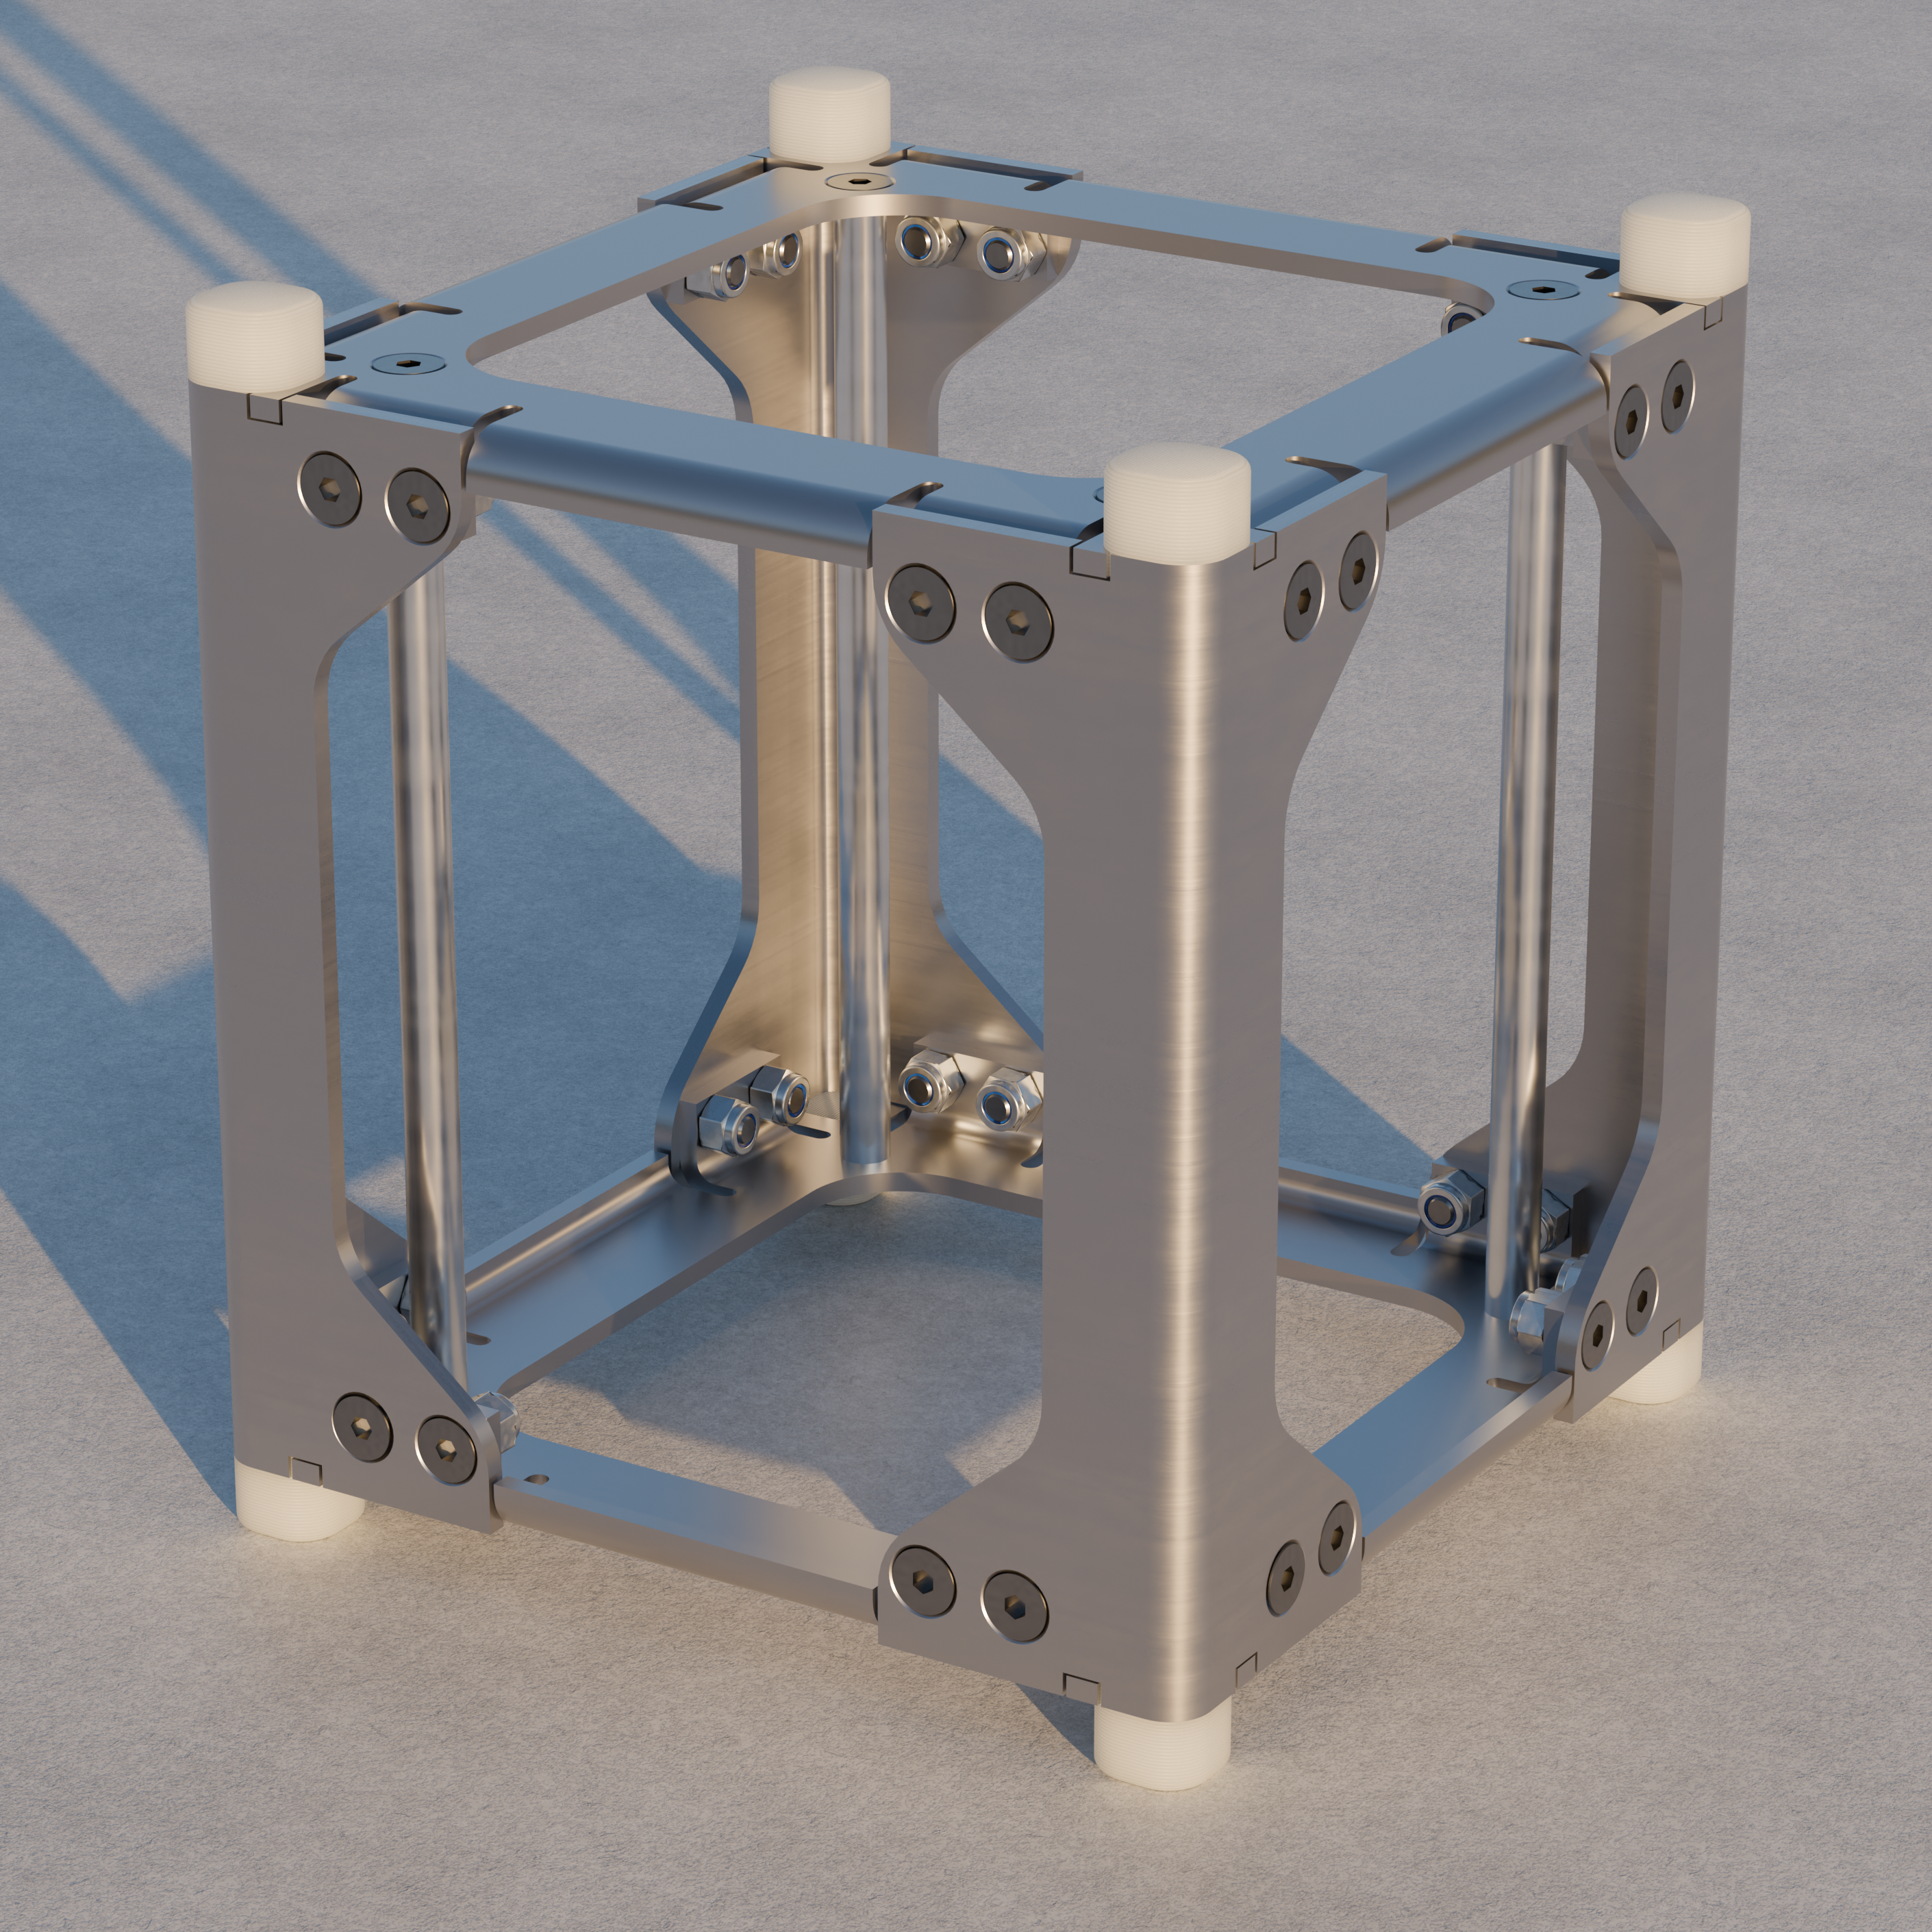
\includegraphics[width=0.6\textwidth]{image/structure/render.png}
      \caption{Renderizado de la estructura propuesta}
      \label{fig:render}
    \end{figure}

    \subsubsection{Descripción General}
      \begin{wrapfigure}{L}{0.4\textwidth}
        \centering
        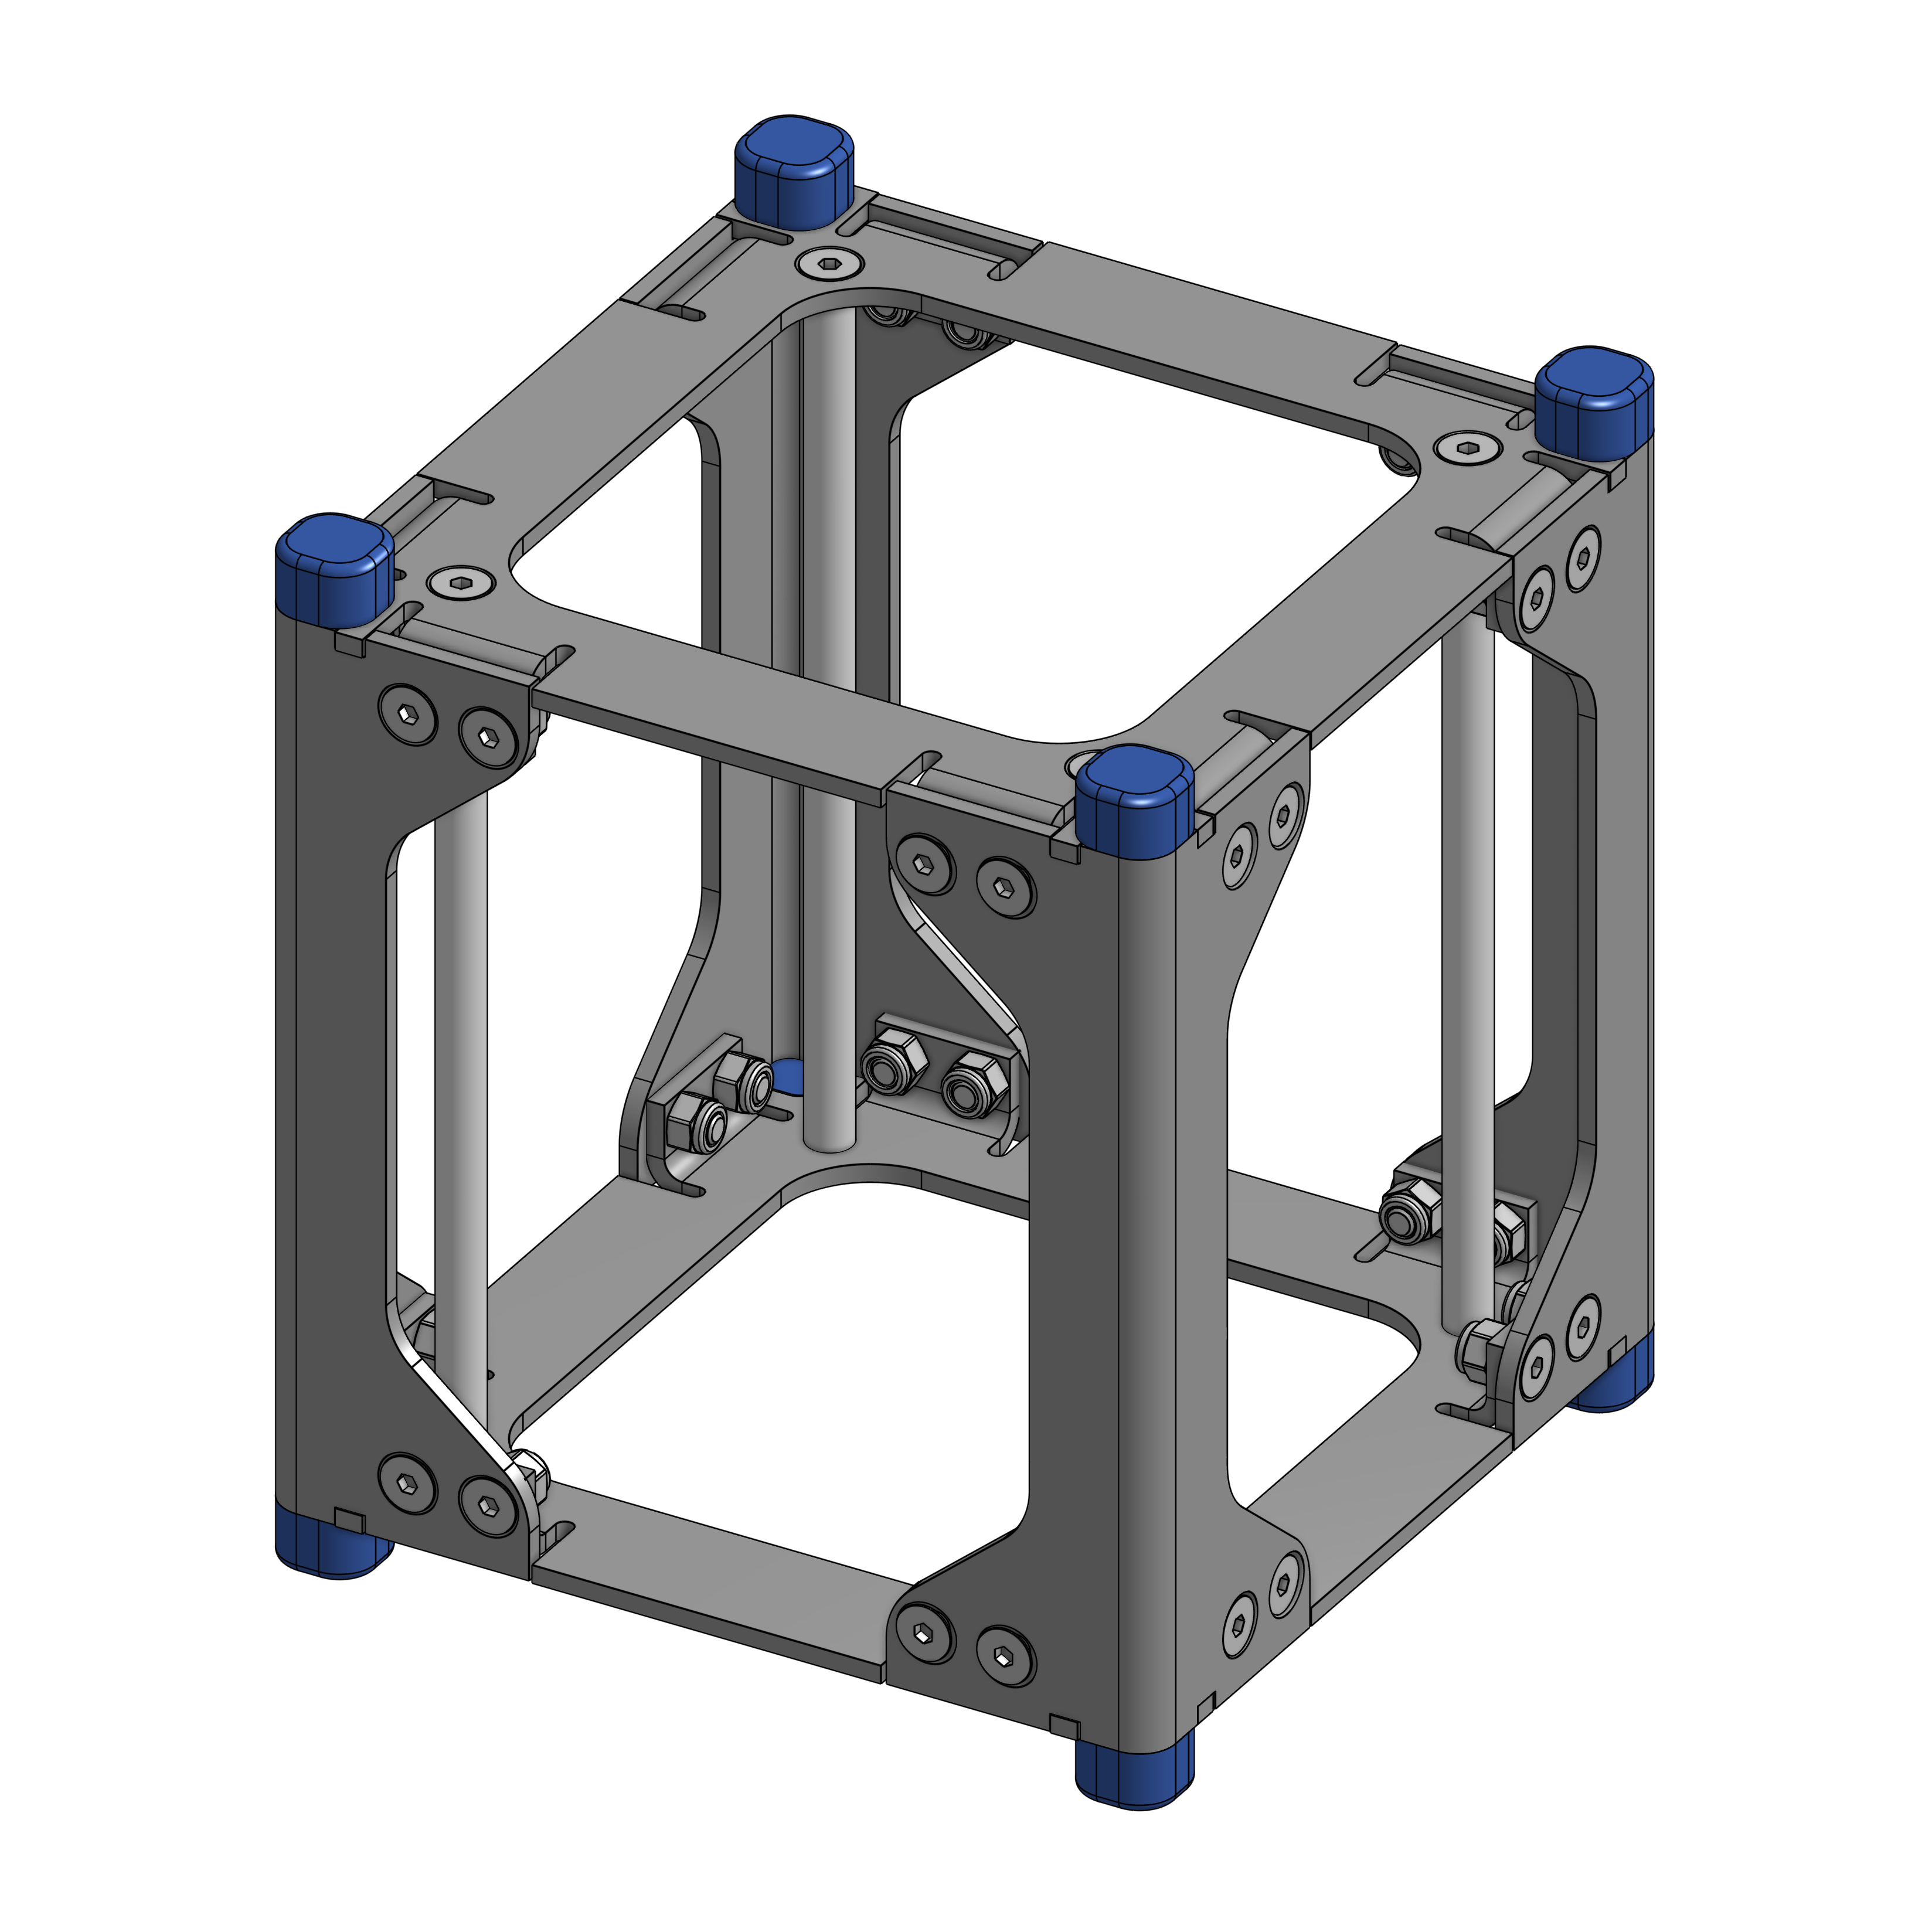
\includegraphics[width=0.4\textwidth]{image/structure/partes.png}
        \caption{Vista trimétrica}
        \label{fig:trimetrica}
      \end{wrapfigure}
      Como se mencionó previamente, la estructura del CubeSat fue diseñada a partir de láminas de aluminio de 2mm de
      espesor plegadas, para maximizar el volumen interno disponible. Esta configuración permite lograr una estructura
      rígida, de fabricación sencilla, y de bajo peso.

      La estructura del CubeSat, consta de 2 tapas, ubicadas en las caras +Z y -Z (lids), unidas a través de 4
      esquineros (corners). La fijación de cada una de estas partes se realiza mediante tornillos y tuercas
      autofrenantes M3. Todos los agujeros de tornillos son avellanados, permitiendo que el CubeSat no tenga
      protuberancias al momento de ensamblarlo.

      \begin{wrapfigure}{R}{0.4\textwidth}
        \centering
        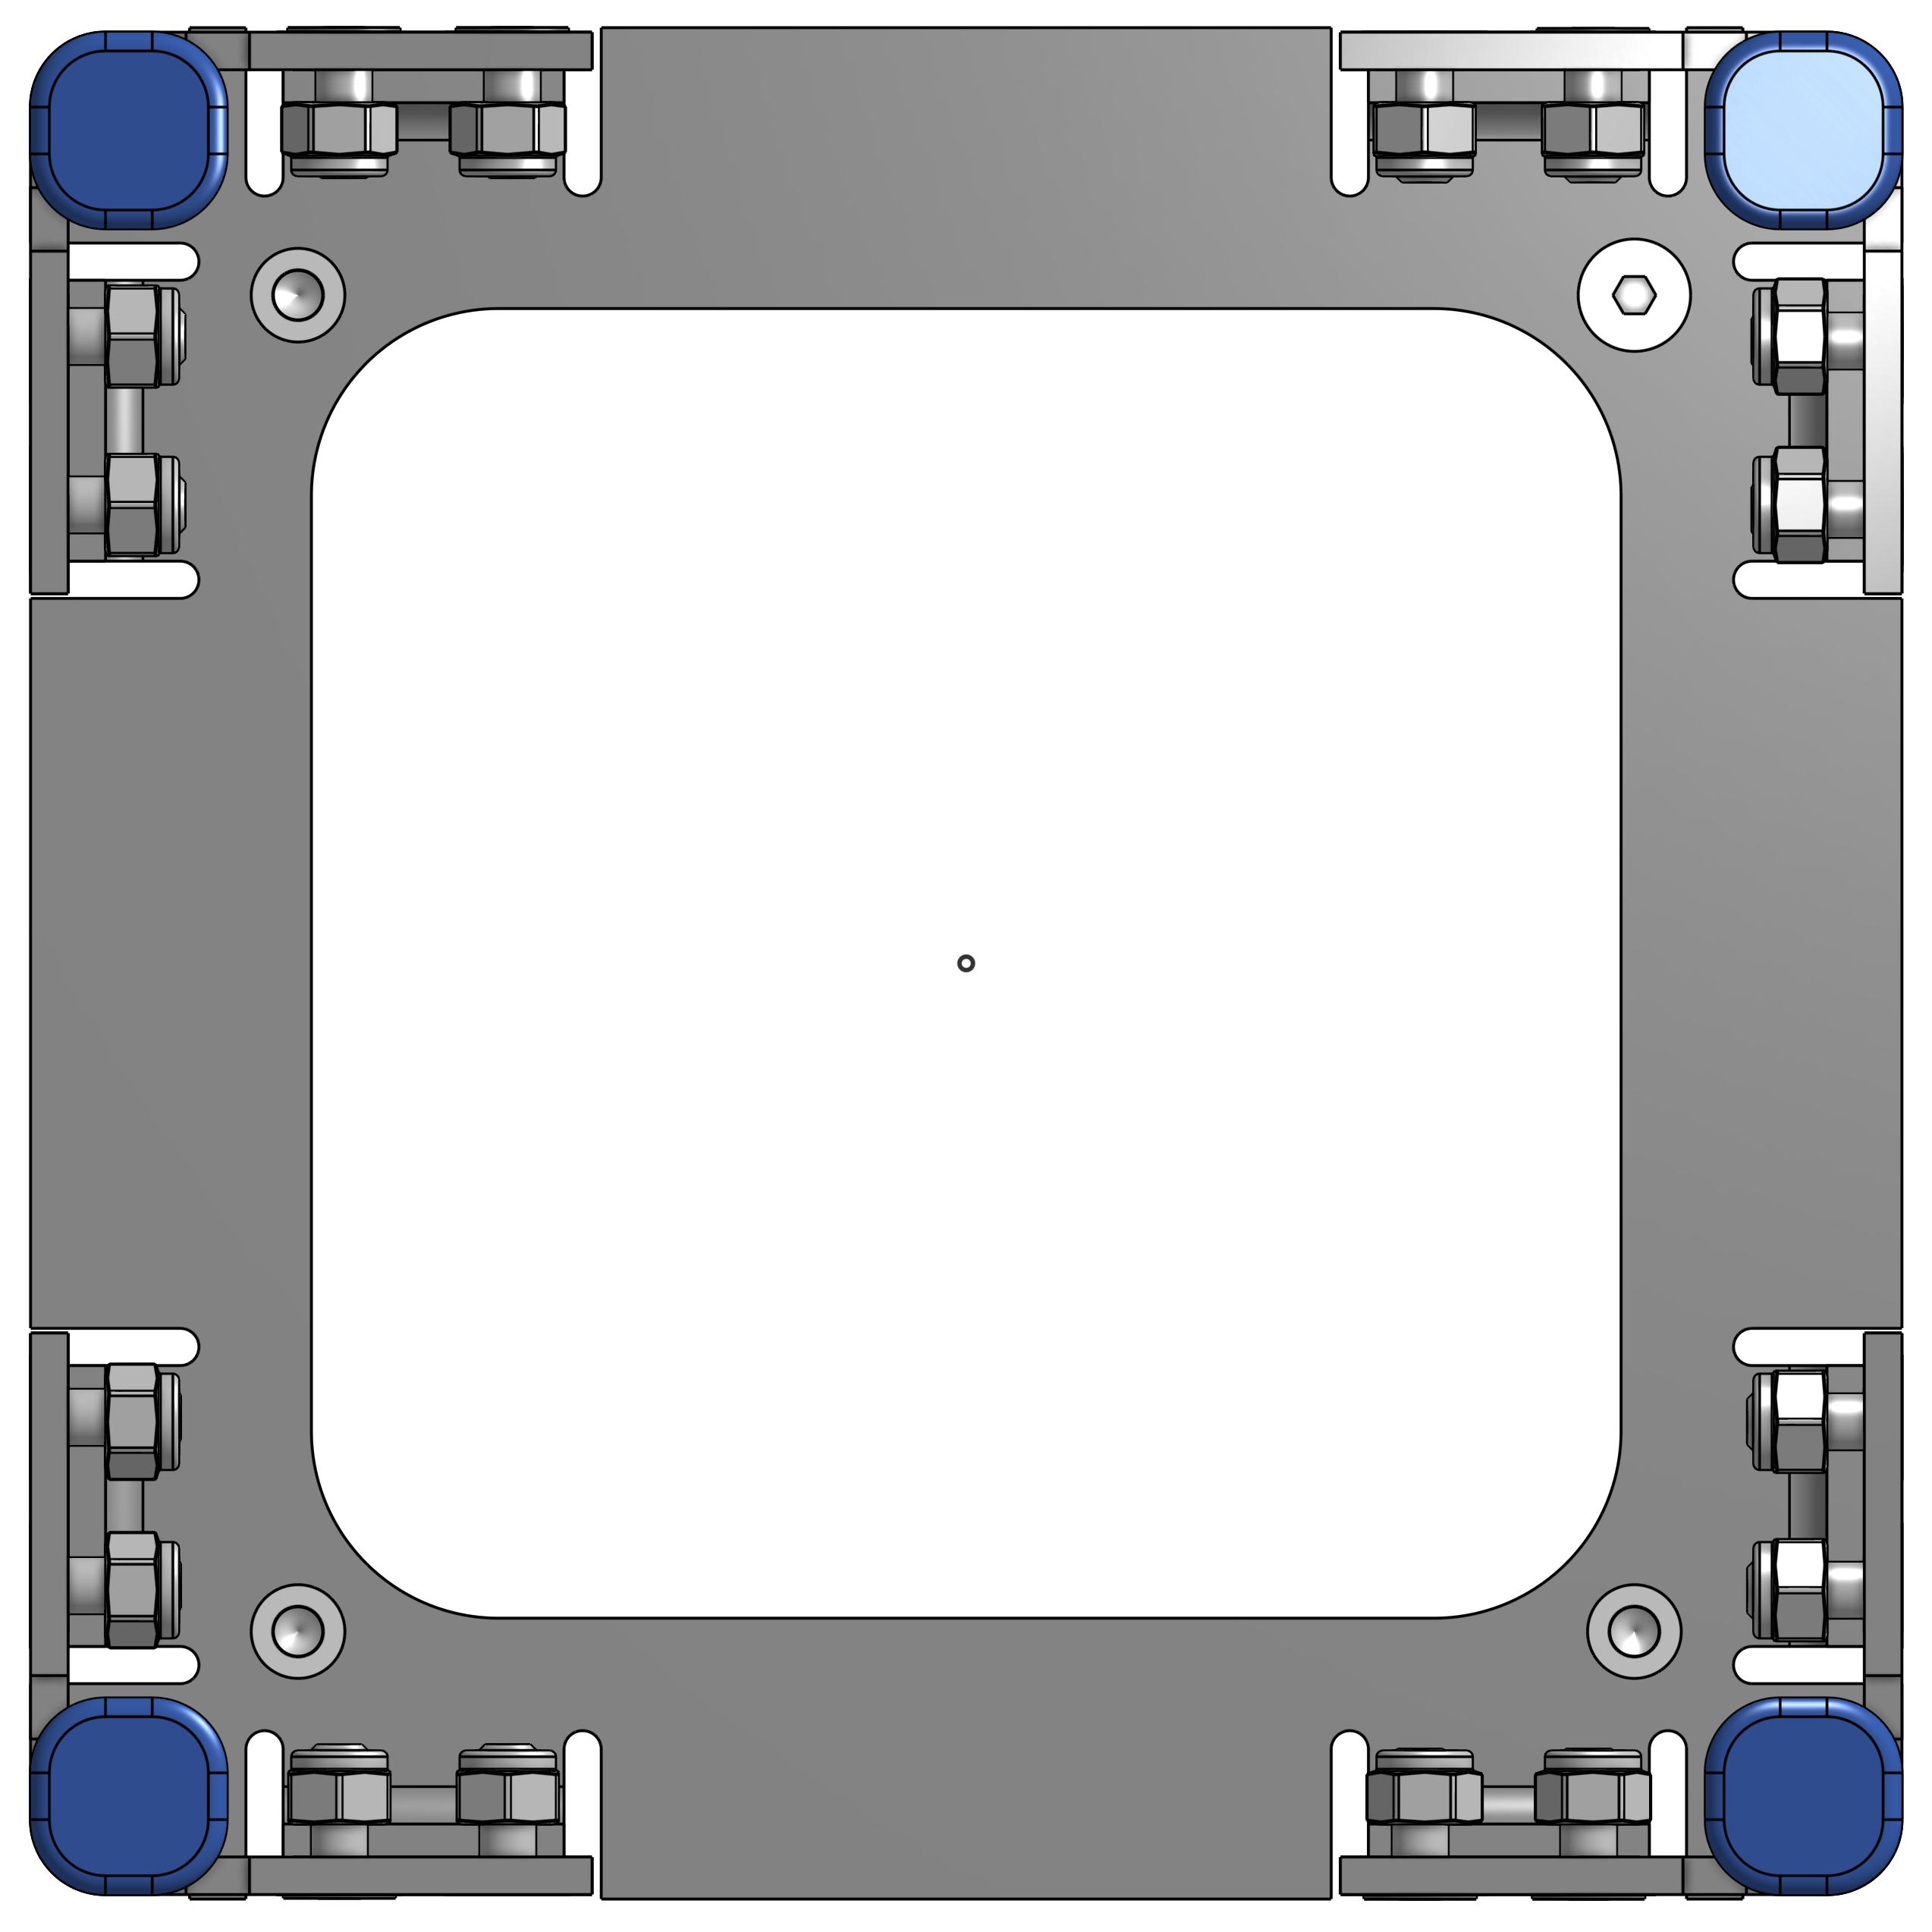
\includegraphics[width=0.4\textwidth]{image/structure/superior.png}
        \caption{Vista superior, sin tapa}
        \label{fig:superior}
      \end{wrapfigure}
      El CubeSat cuenta con ocho puntos de apoyo ubicados en las caras +Y y -Y (sides), fabricados mediante
      impresión 3D por Modelado por Deposición Fundida (FDM) en polipropileno, un material que se seleccionó por su baja
      densidad, lo cual reduce la masa total del sistema, y por su buena capacidad de sellado y excelente adherencia
      entre capas, permitiendo que los modulos internos del CubeSat puedan ser hermeticos.

      El CubeSat alberga diferentes modulos, los cuales sirven para proveer una separacion fisica entre diferentes
      subsistemas. Los modulos ocupan todo el espacio disponible en el plano XY. Esto es para no necesitar fijar los
      diferentes modulos a la estructura con tornilleria. La altura de cada módulo está pensada en base a lo que
      alberga, y entre todos los modulos se completa el espacio disponible en el eje Z, por lo que cuando el CubeSat
      está completamente ensamblado, no hay espacio para que los modulos se desplacen en el eje Z.

      Los diferentes modulos se colocan de forma segura en sus correspondientes espacios en la estructura, y sé
      imprimen por separado utilizando la técnica de impresión 3D (FDM) en polipropileno, que tiene muy buenas
      propiedades de adherencia entre capas, permitiendo (en caso de ser necesario) crear volúmenes que sean herméticos.

    \subsubsection{Dimensiones y referencias}
      Revisar la seccion \ref{anexo:planos.estructura} para ver planos con vistas principales, dimensiones y pata de
      referencia.

    \subsubsection{Proceso de Integración}
      El armado del CubeSat, comienza con la colocación de la tapa inferior (plano -Z) sobre el banco de armado, con los
      pliegues hacia arriba. A estos pliegues, se le colocan las cuatro esquinas, fijándolas con los tornillos y tuercas
      autobloqueantes. Una vez colocados las cuatro esquinas, se puede colocar las varillas en la cara
      interna de la tapa inferior (plano -Z), utilizando los tornillos correspondientes.
      
      \begin{figure}[H]
        \begin{minipage}{0.4\textwidth}
          \centering
          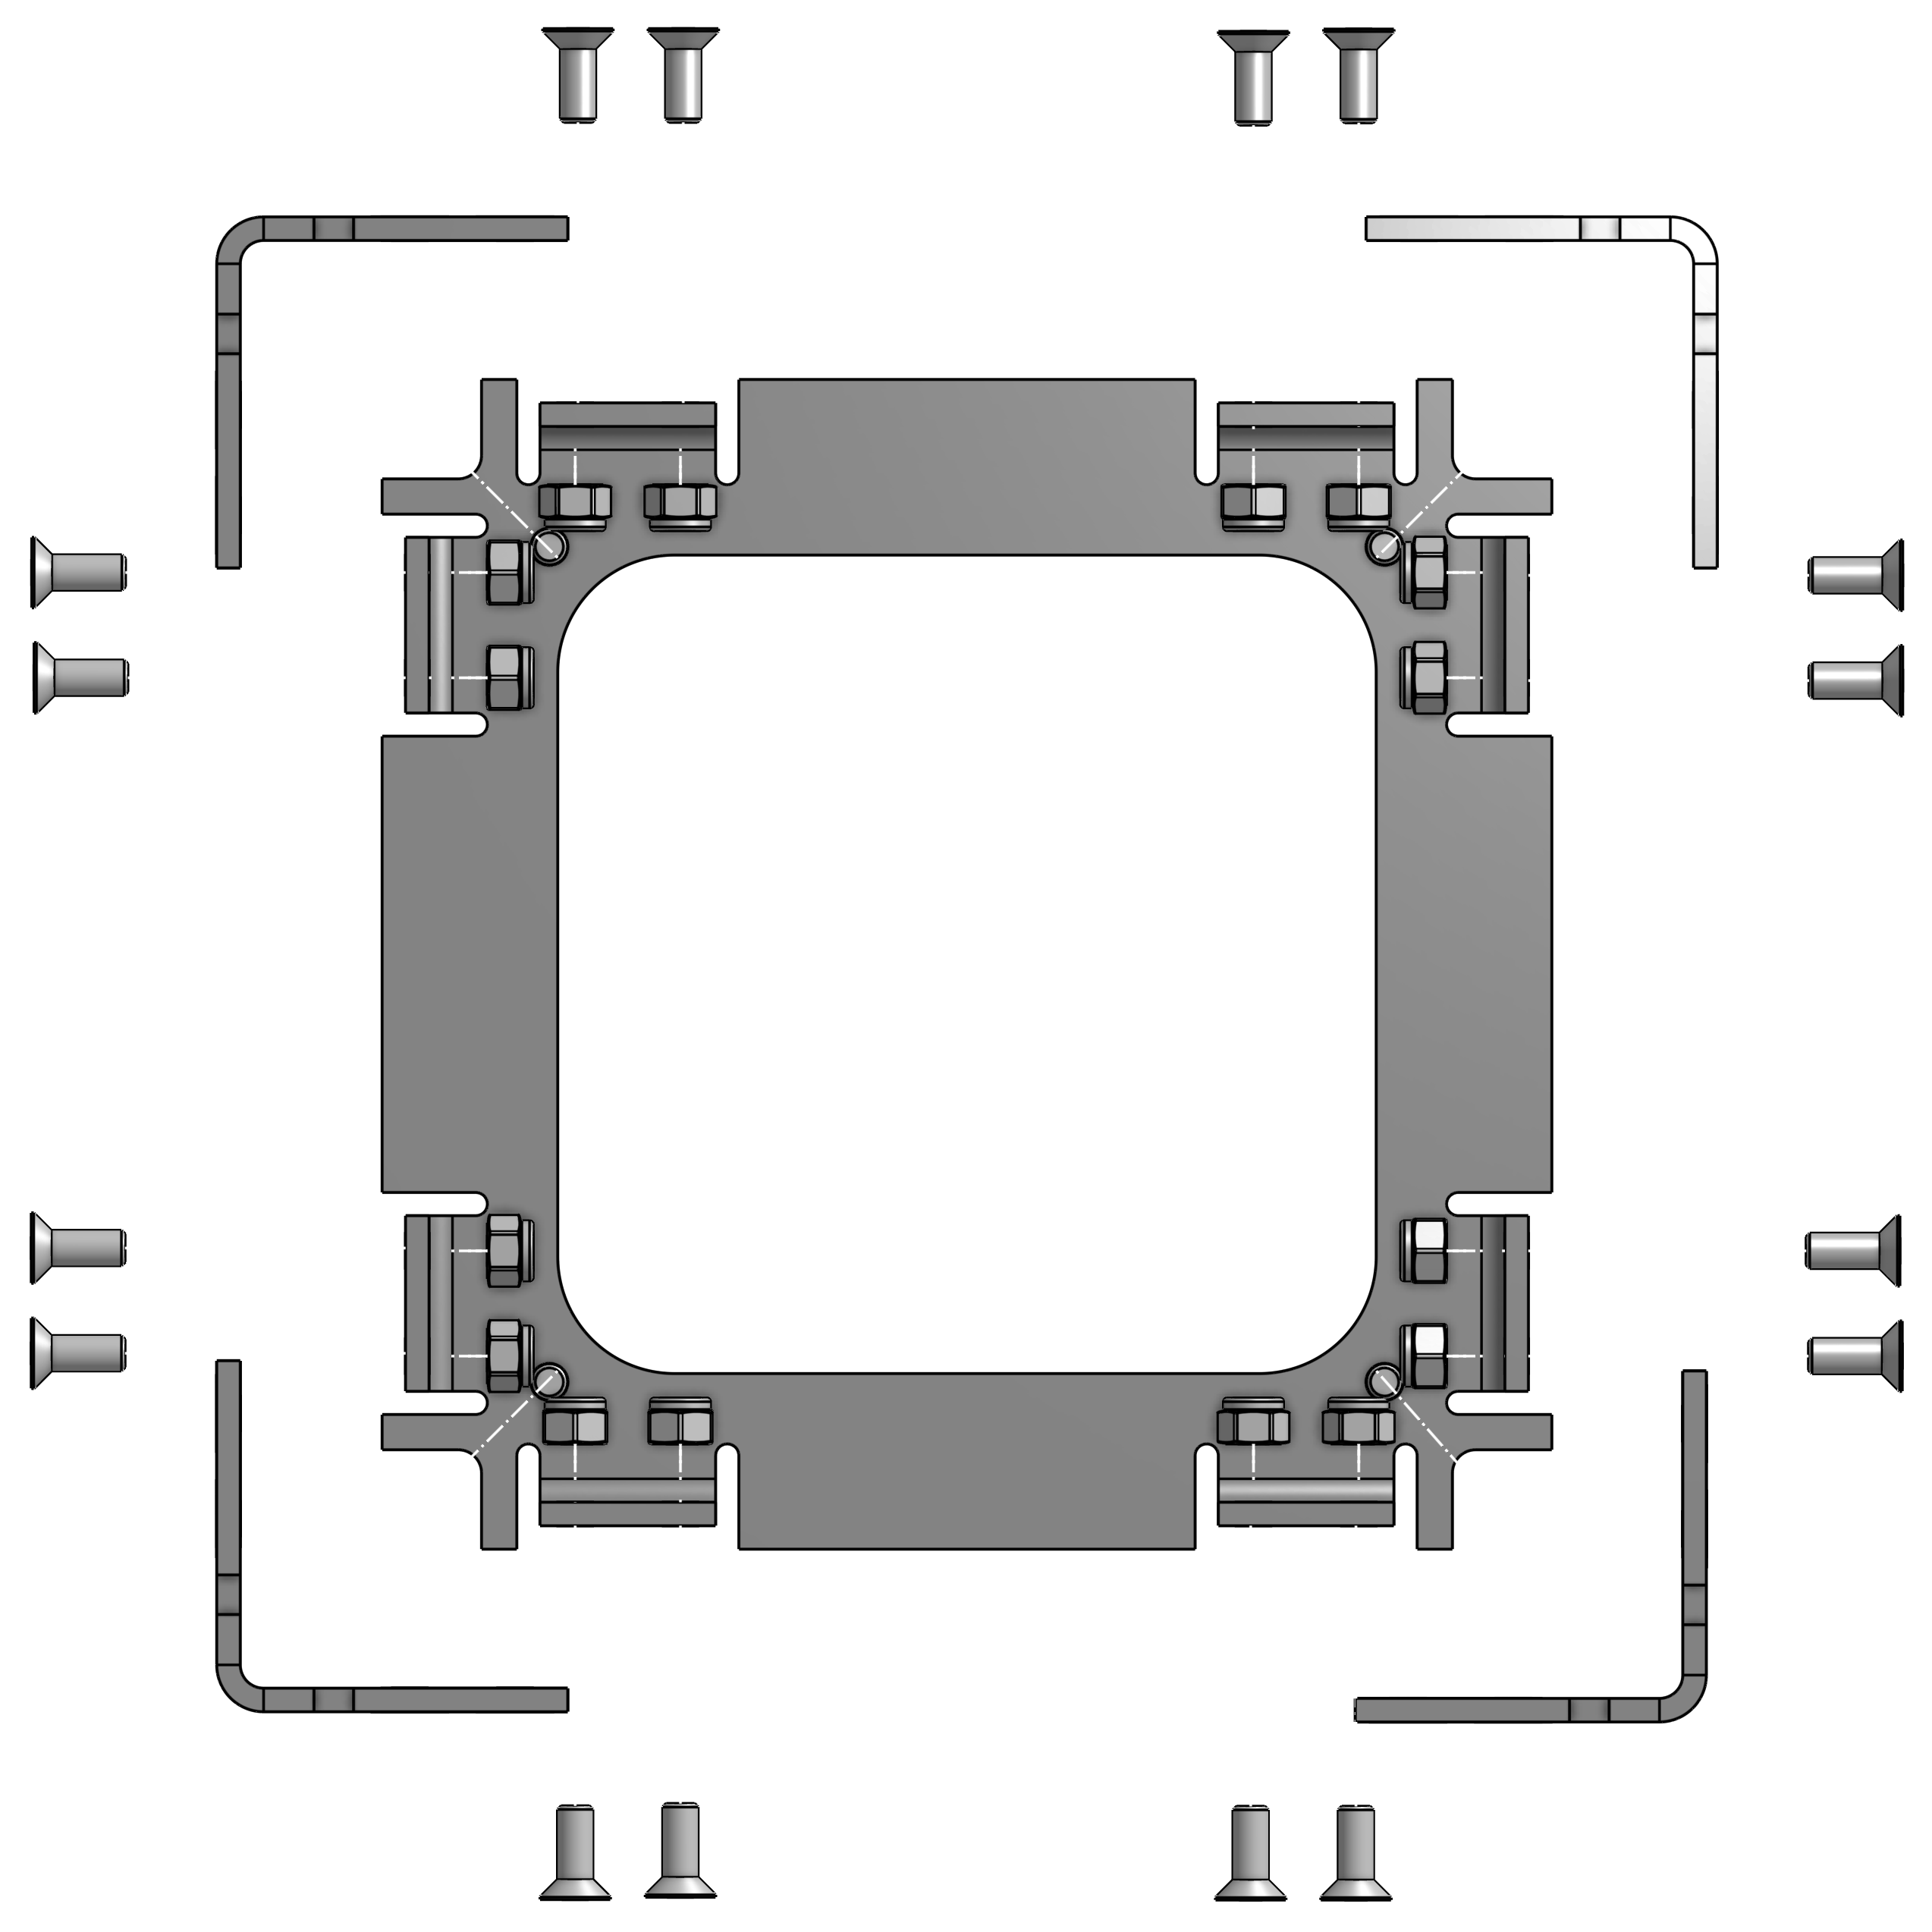
\includegraphics[width=1\textwidth]{image/structure/integracion1.png}
          \caption{Integración paso 1}
          \label{fig:integracion1}
        \end{minipage}
        \hfill
        \begin{minipage}{0.4\textwidth}
          \centering
          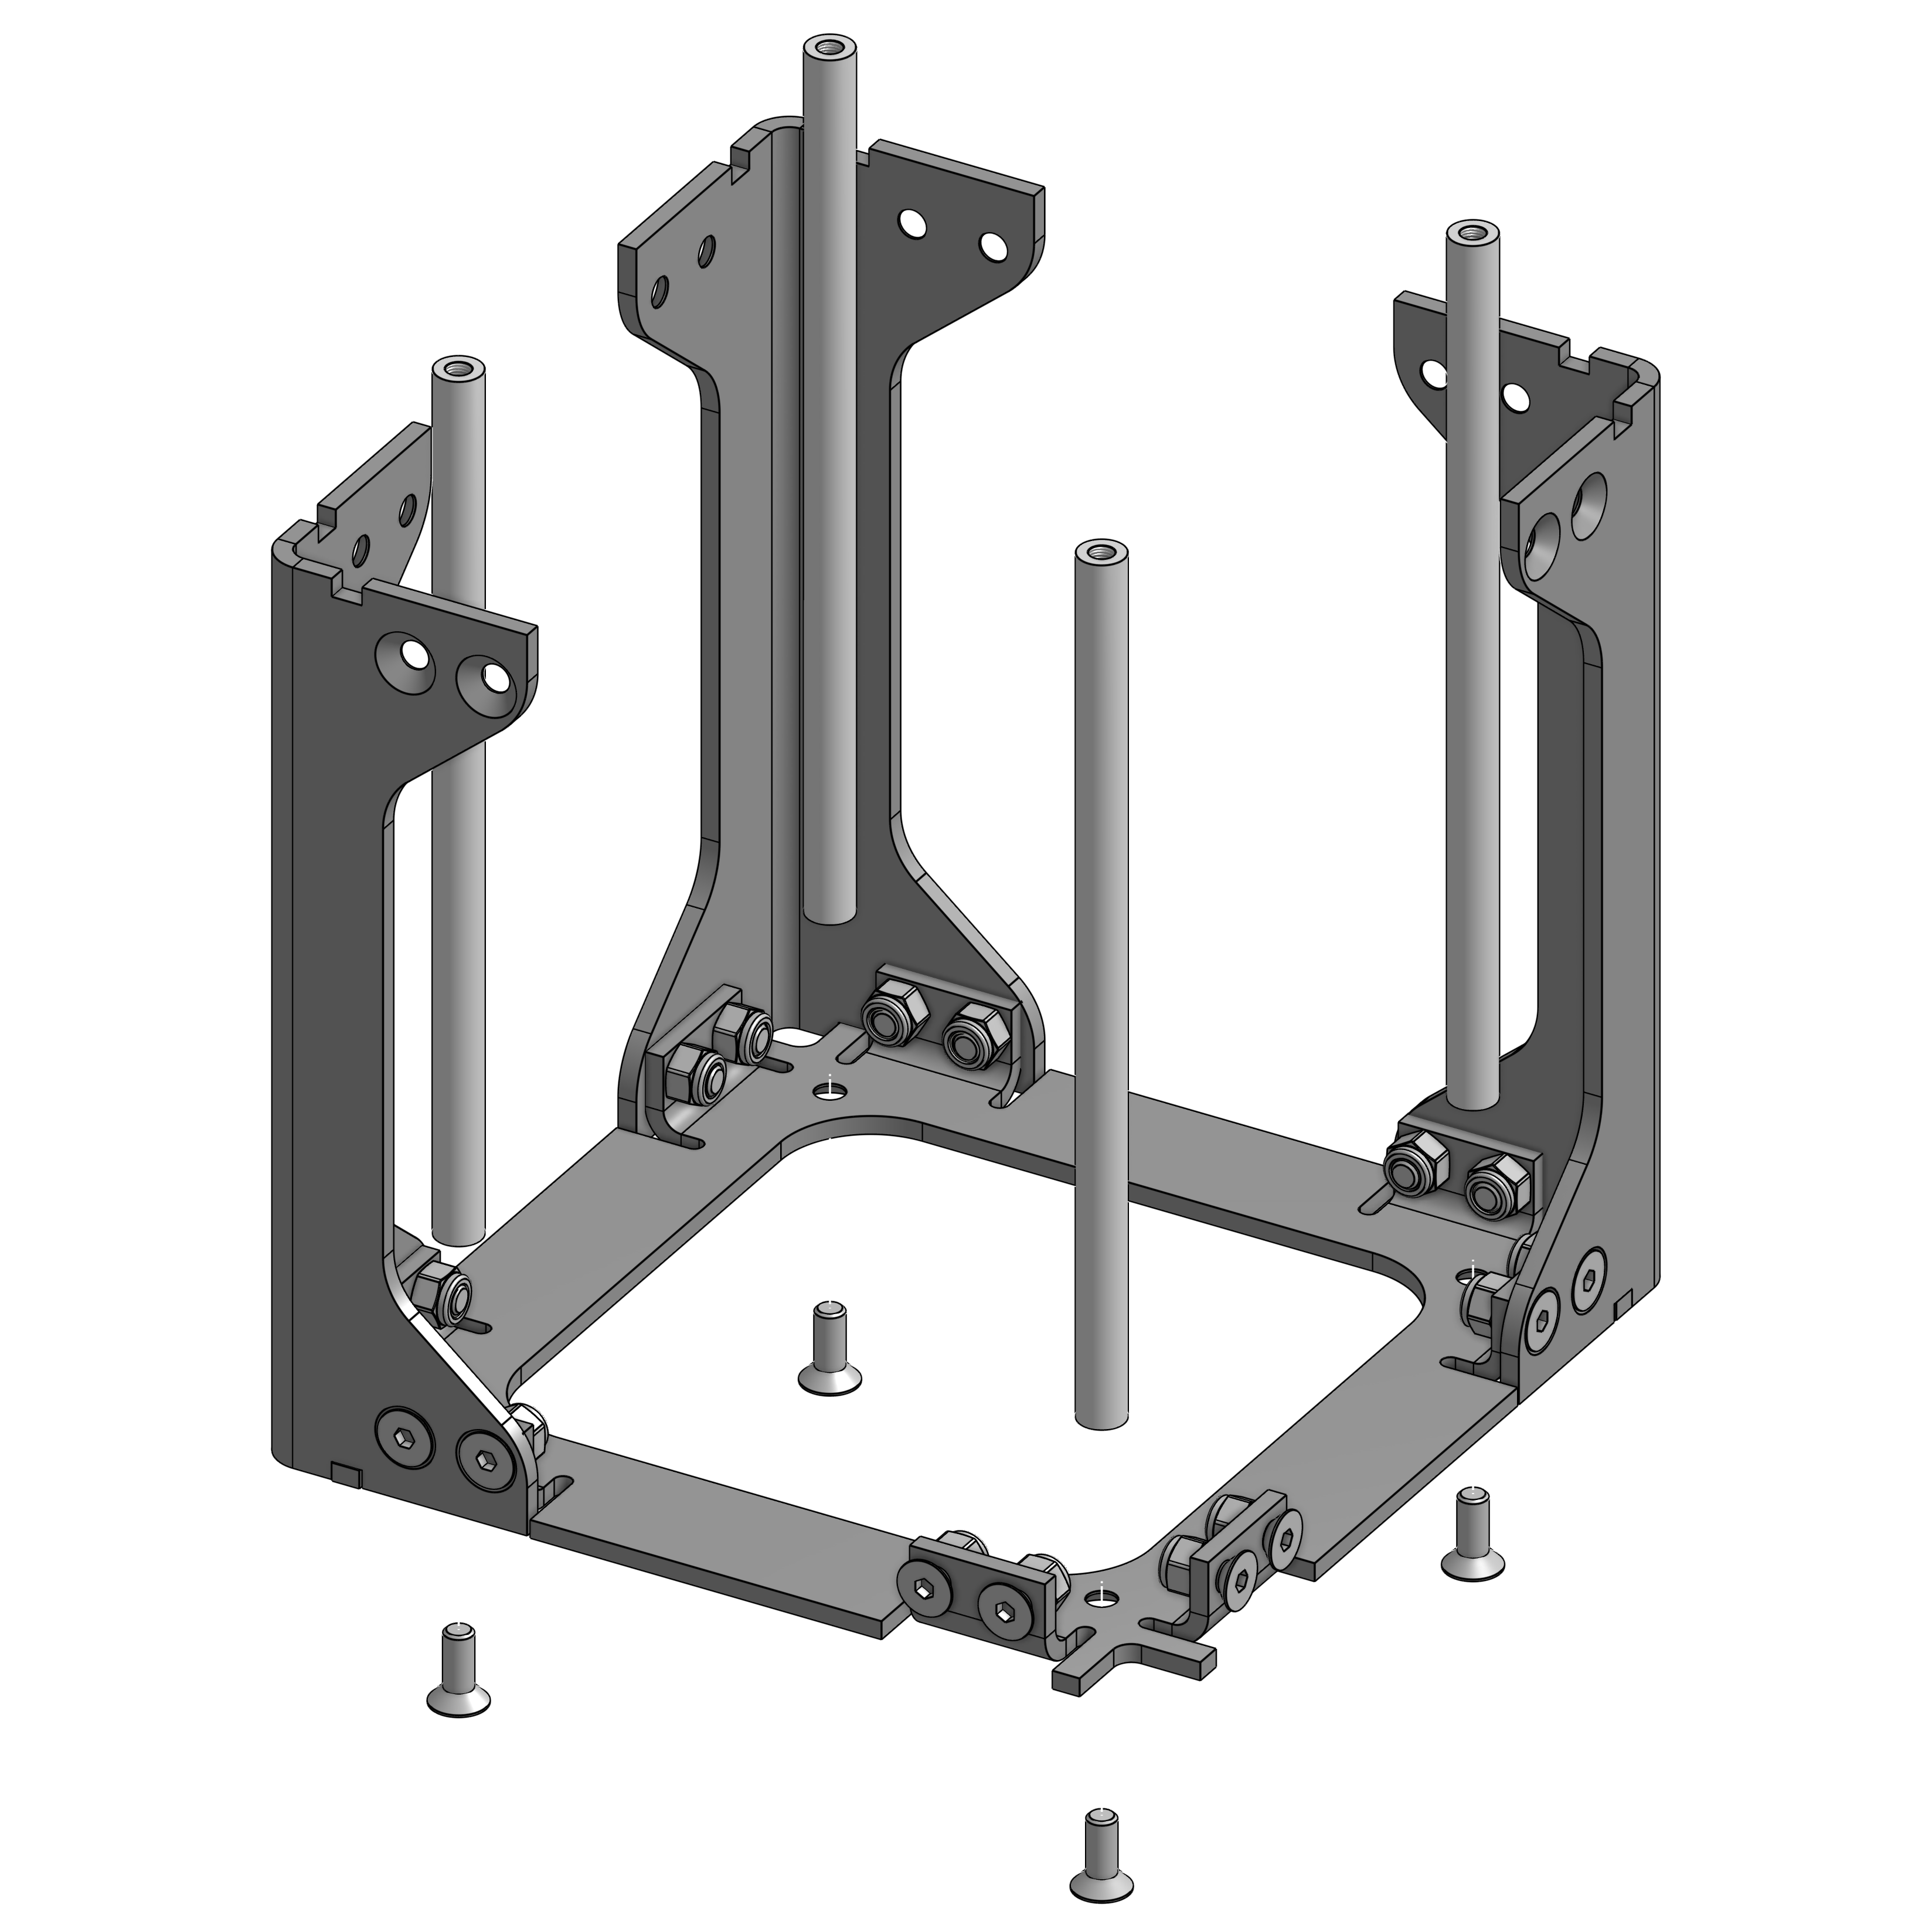
\includegraphics[width=1\textwidth]{image/structure/integracion2.png}
          \caption{Integración paso 2}
          \label{fig:integracion2}
        \end{minipage}
      \end{figure}

      Después de haber colocado las varillas, se puede colocar los diferentes modulos uno por uno,
      conectándolos entre sí. Luego se coloca la tapa superior (plano +Z), se fijan las varillas con los tornillos.
      Utilizando la herramienta de ajuste diseñada para acceder a las tuercas superiores, se colocan los tornillos con
      las tuercas autobloqueantes respetando el orden de esquina al centro.

      \begin{figure}[H]
        \begin{minipage}{0.49\textwidth}
          \centering
          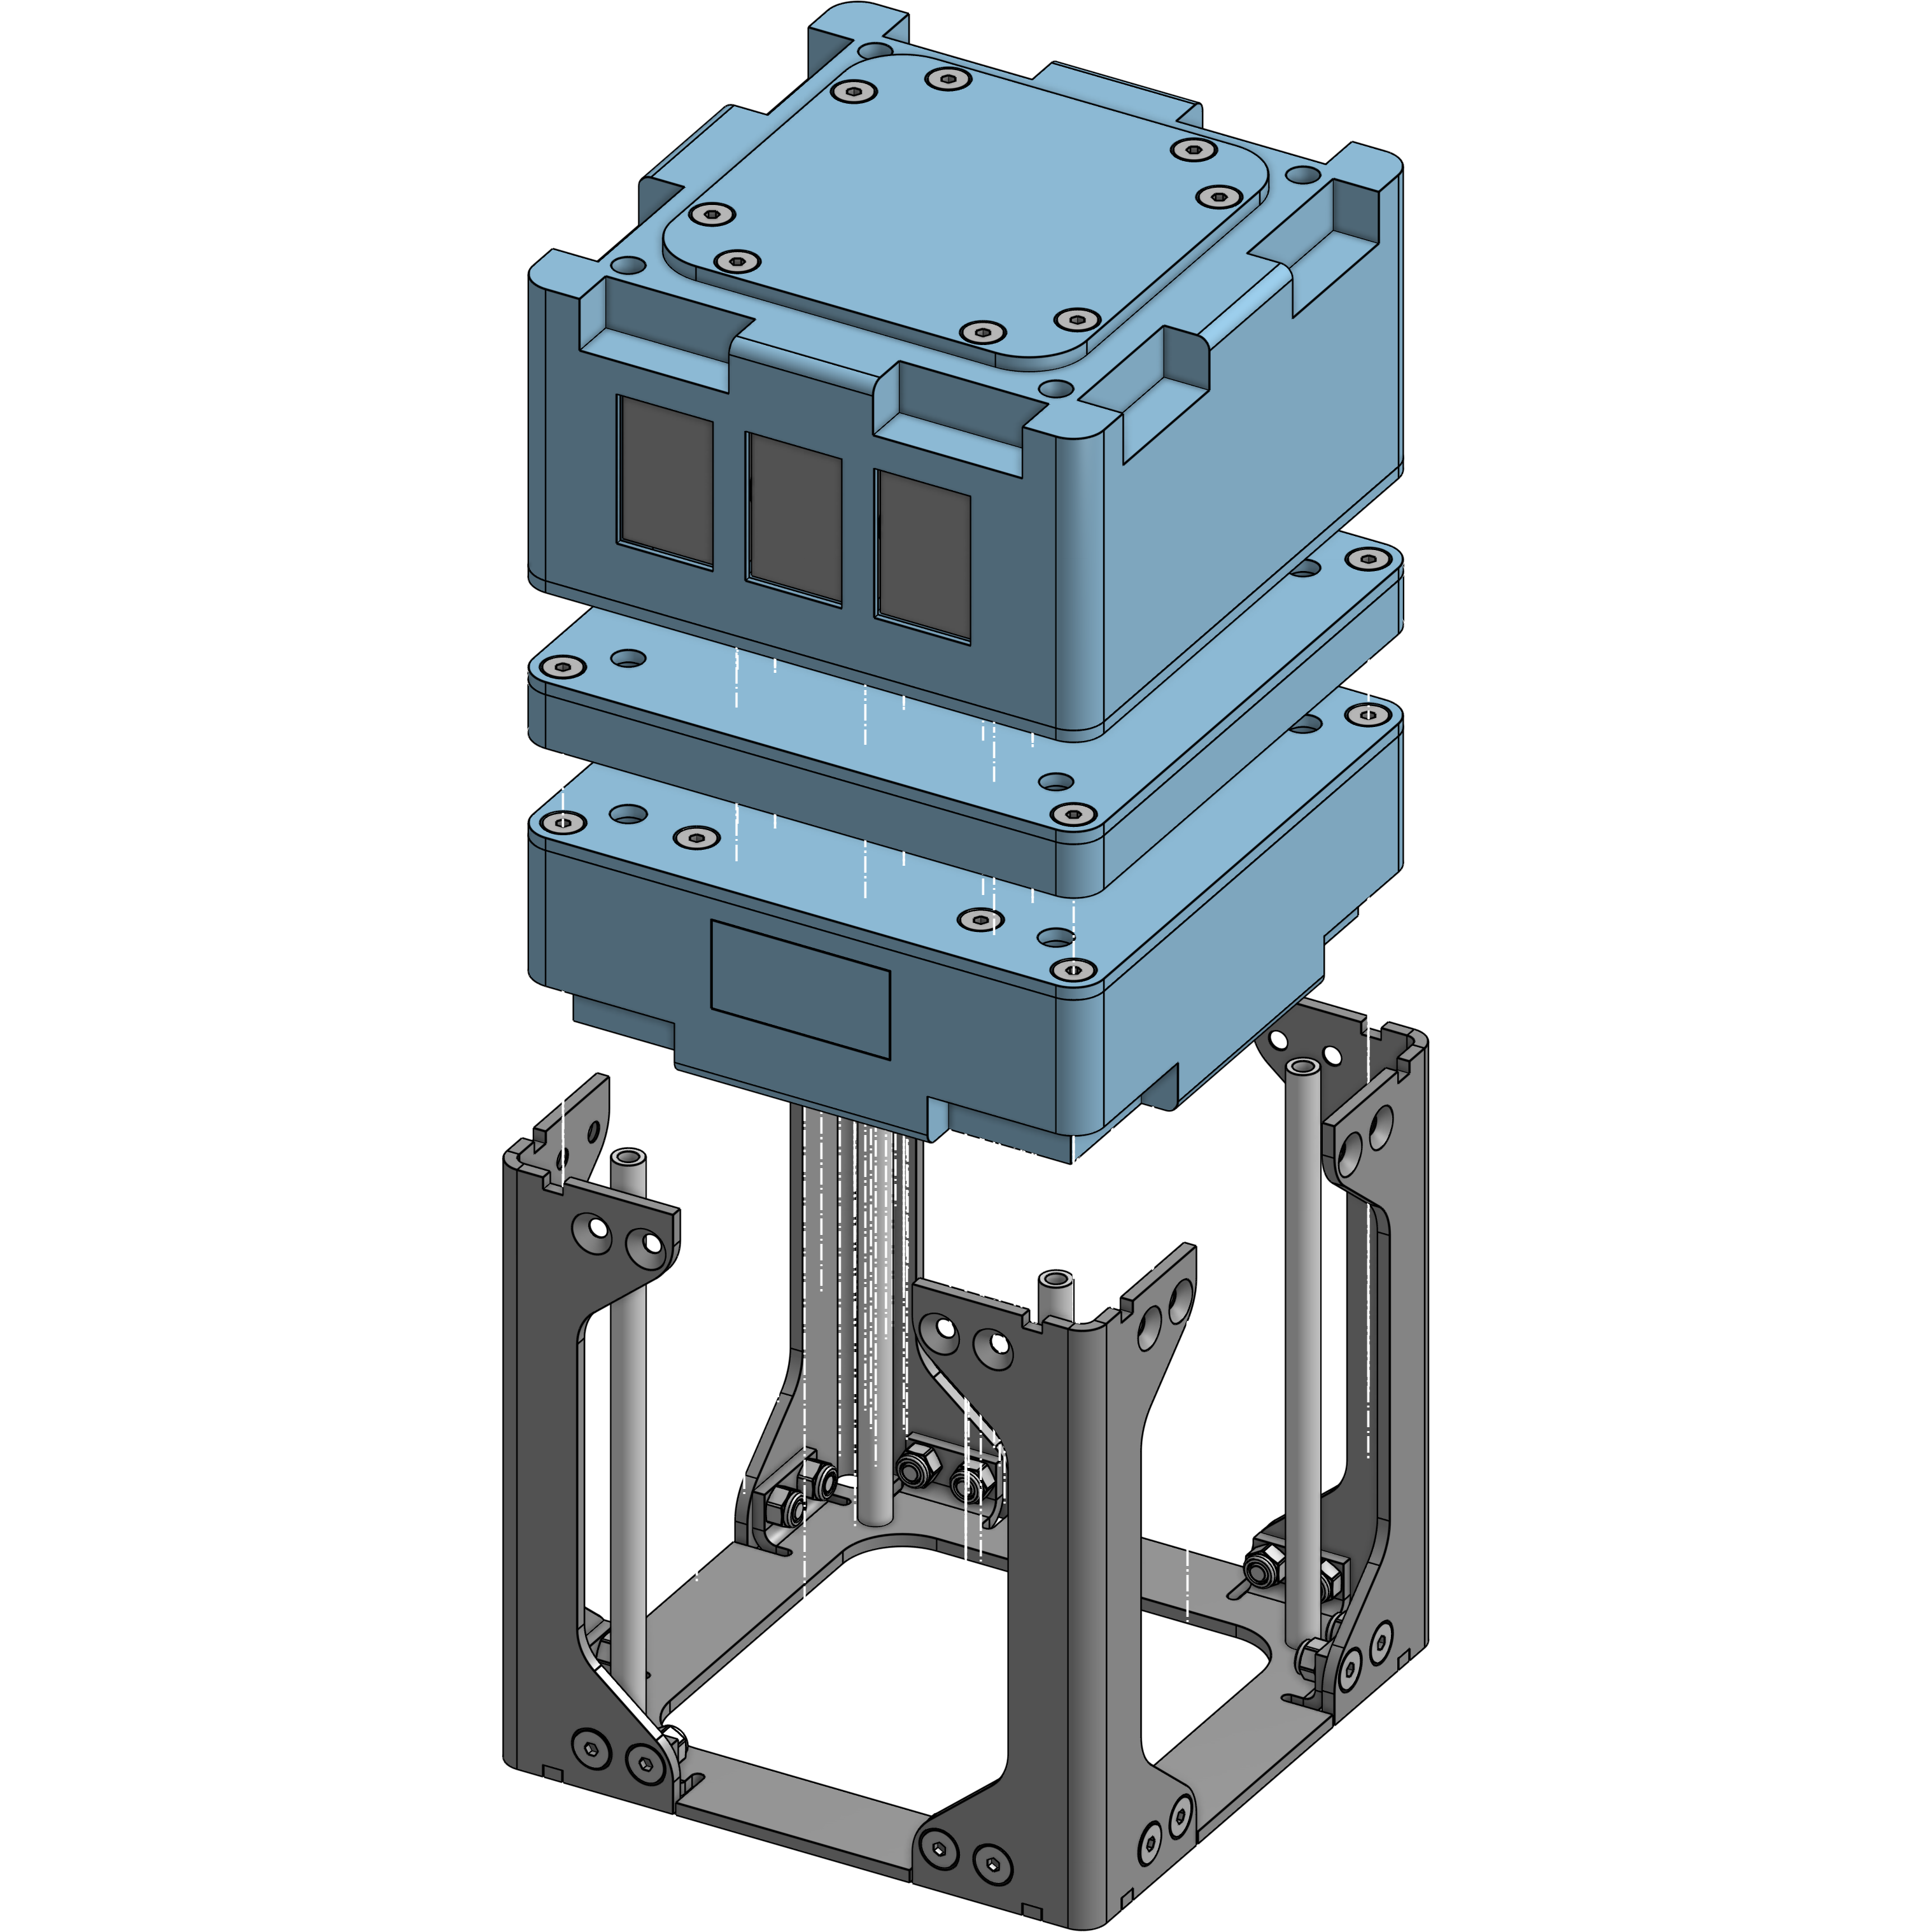
\includegraphics[width=0.9\textwidth]{image/structure/integracion3.png}
          \caption{Integración paso 3}
          \label{fig:integracion3}
        \end{minipage}
        \begin{minipage}{0.49\textwidth}
          \centering
          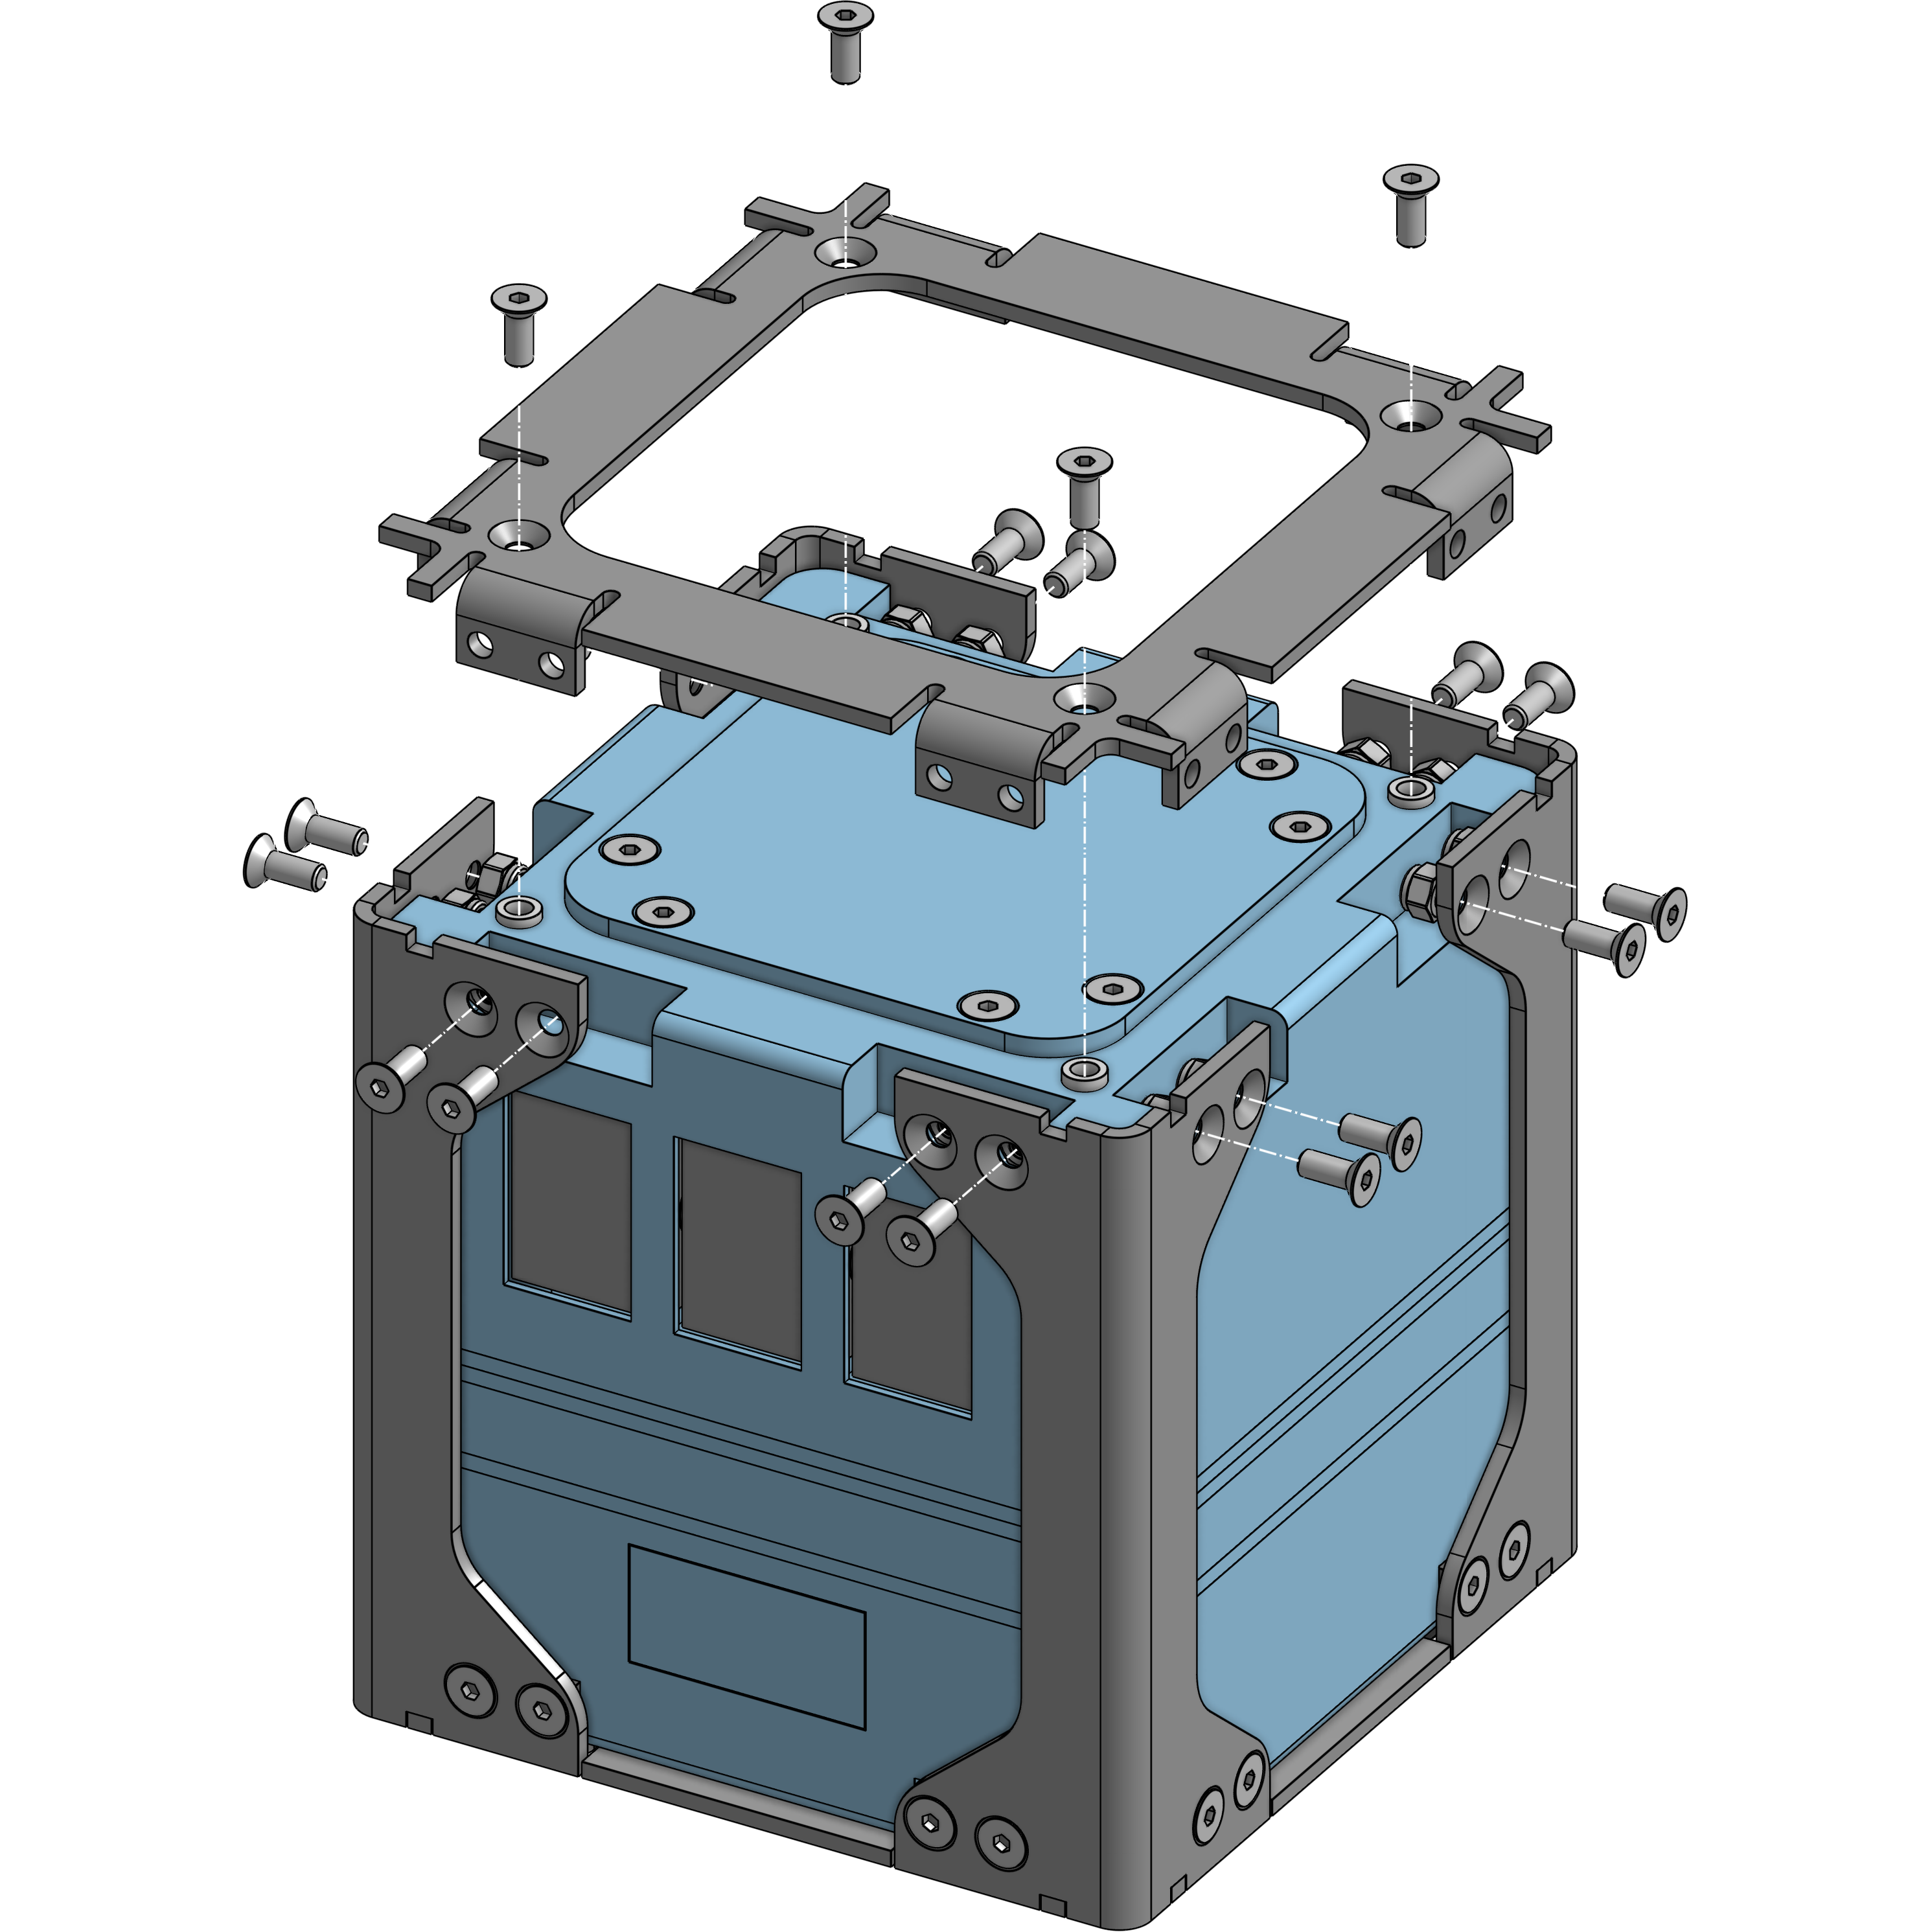
\includegraphics[width=0.9\textwidth]{image/structure/integracion4.png}
          \caption{Integración paso 4}
          \label{fig:integracion4}
        \end{minipage}
      \end{figure}

      Finalmente, se colocan los rieles a presión, para asegurar una sujeción firme estos deben ser enfriados
      previamente.
      \begin{figure}[H]
        \centering
        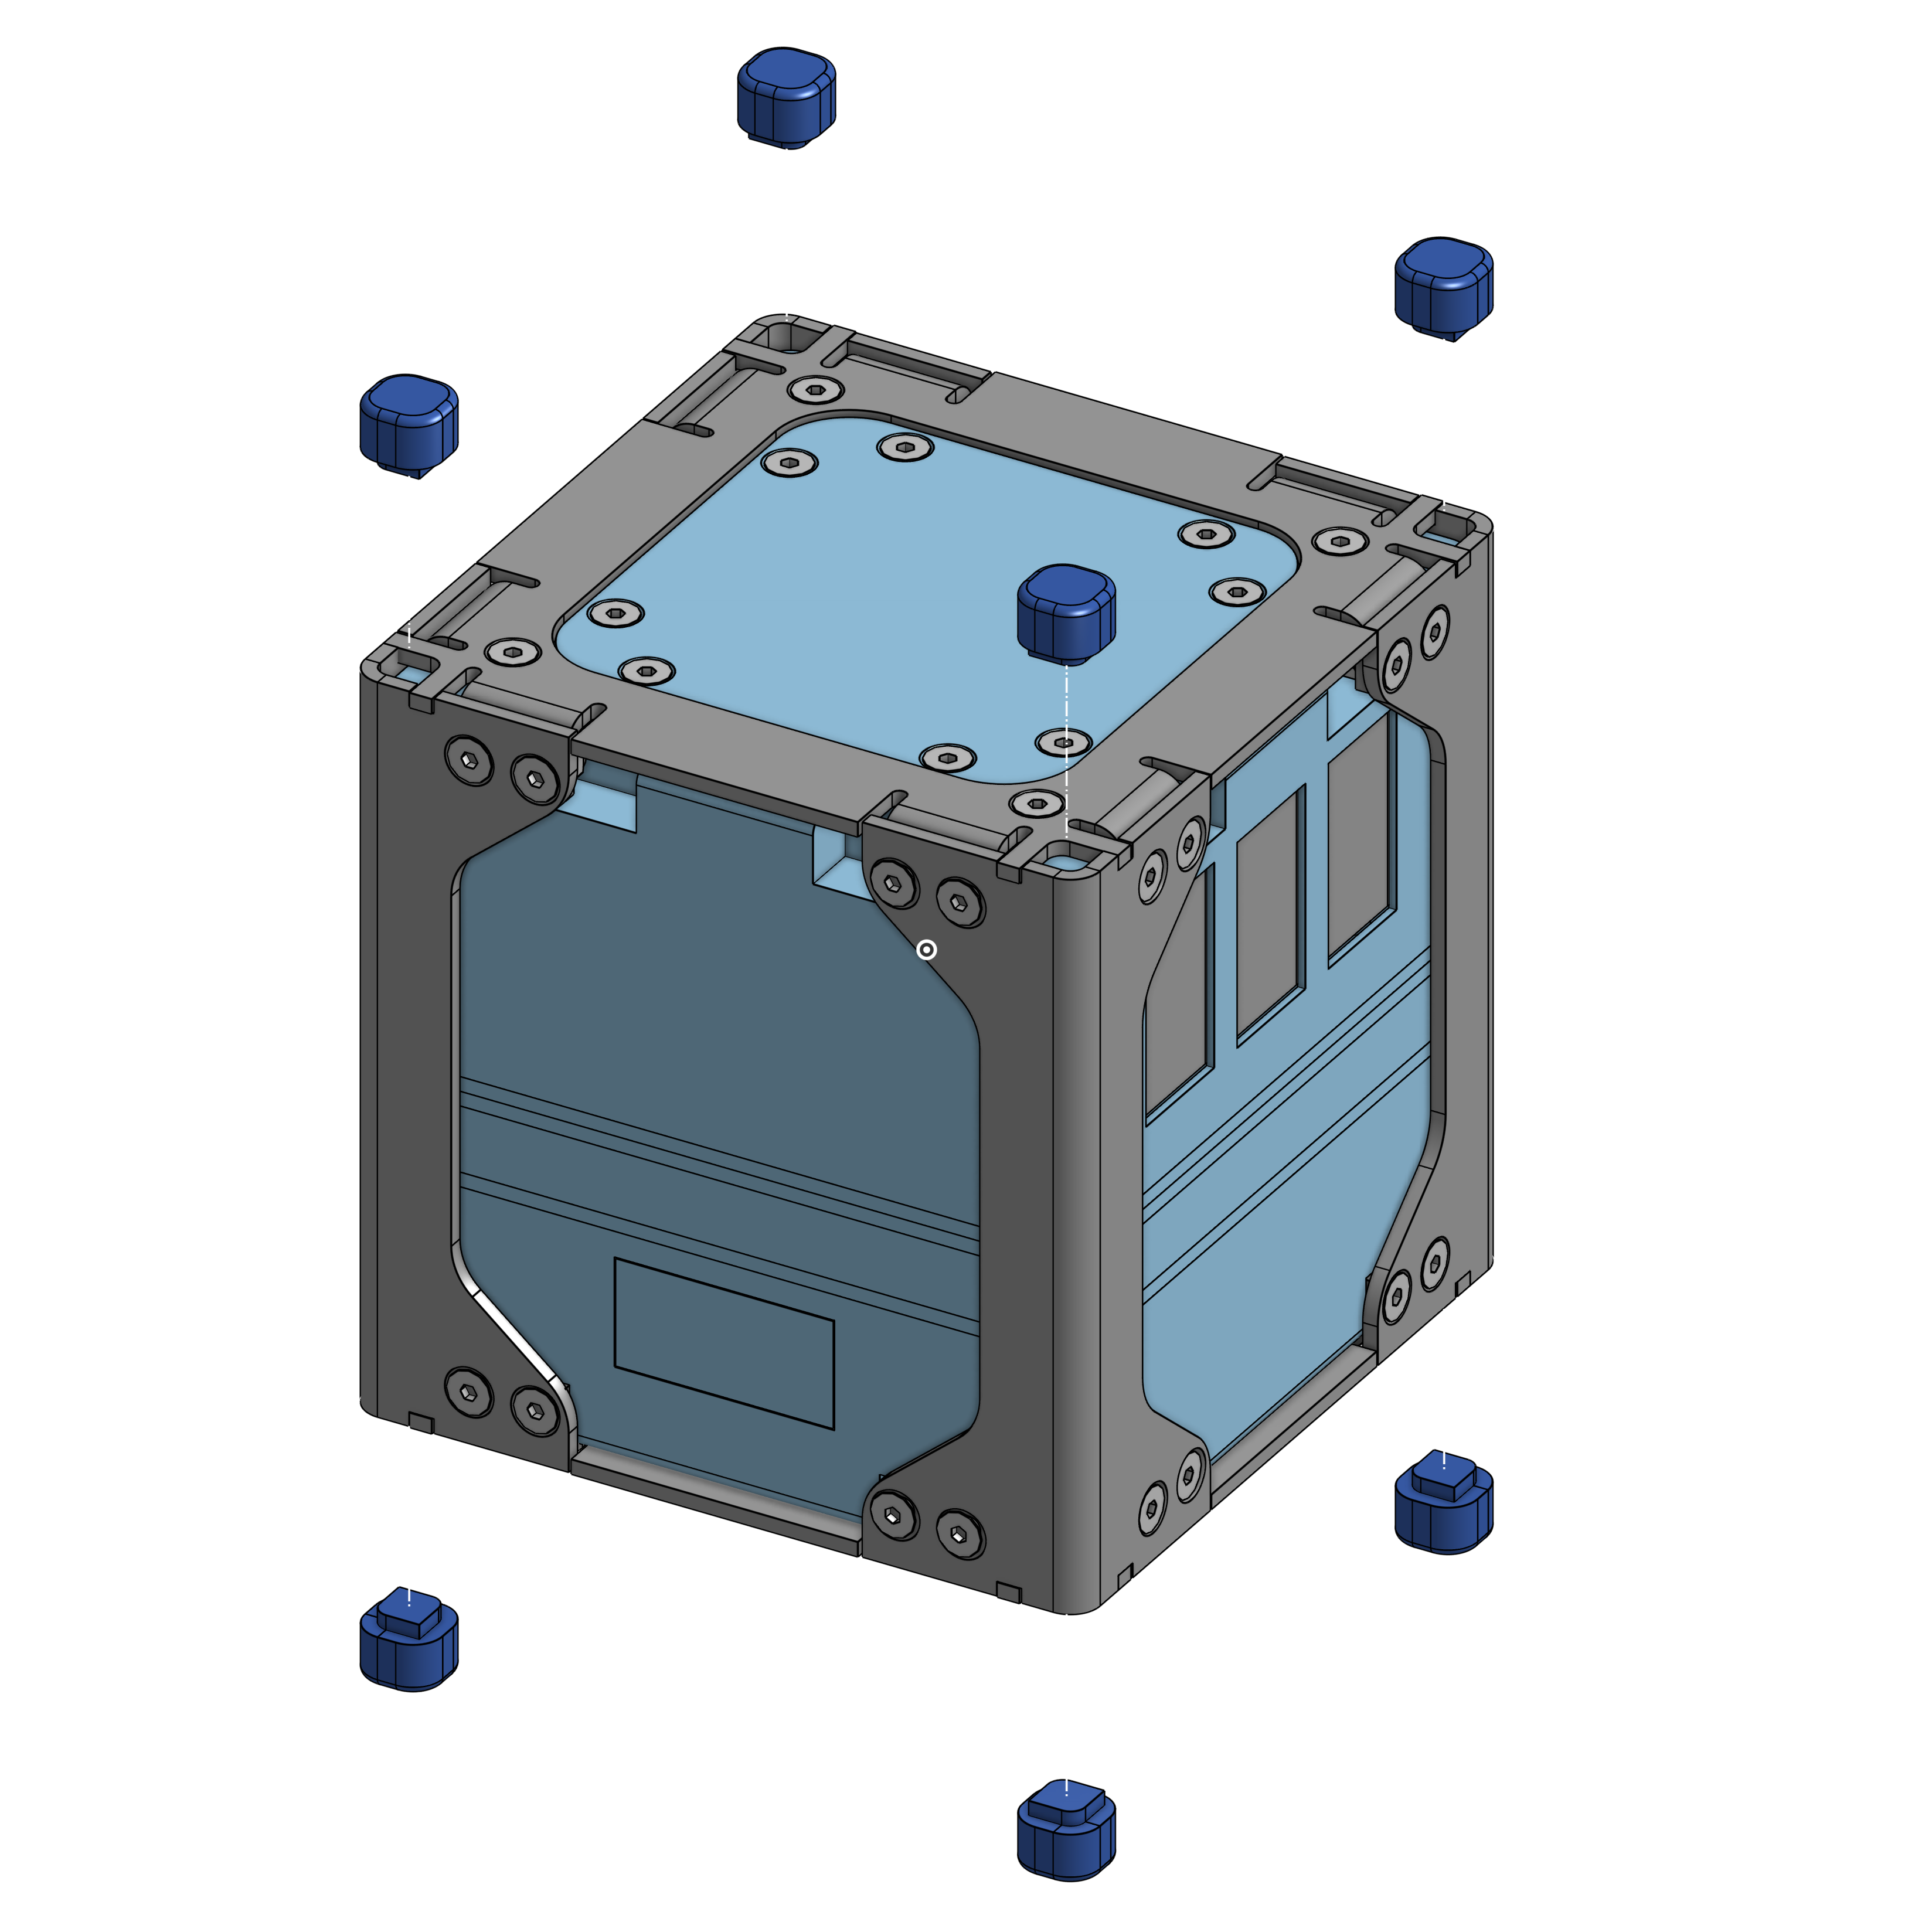
\includegraphics[width=0.4\textwidth]{image/structure/integracion5.png}
        \caption{Integración paso 5}
        \label{fig:integracion5}
      \end{figure}
      \newpage

    \subsubsection{Módulo \acrshort{pms}}
      \begin{wrapfigure}{R}{0.35\textwidth}
        \vspace{-1cm}
        \centering
        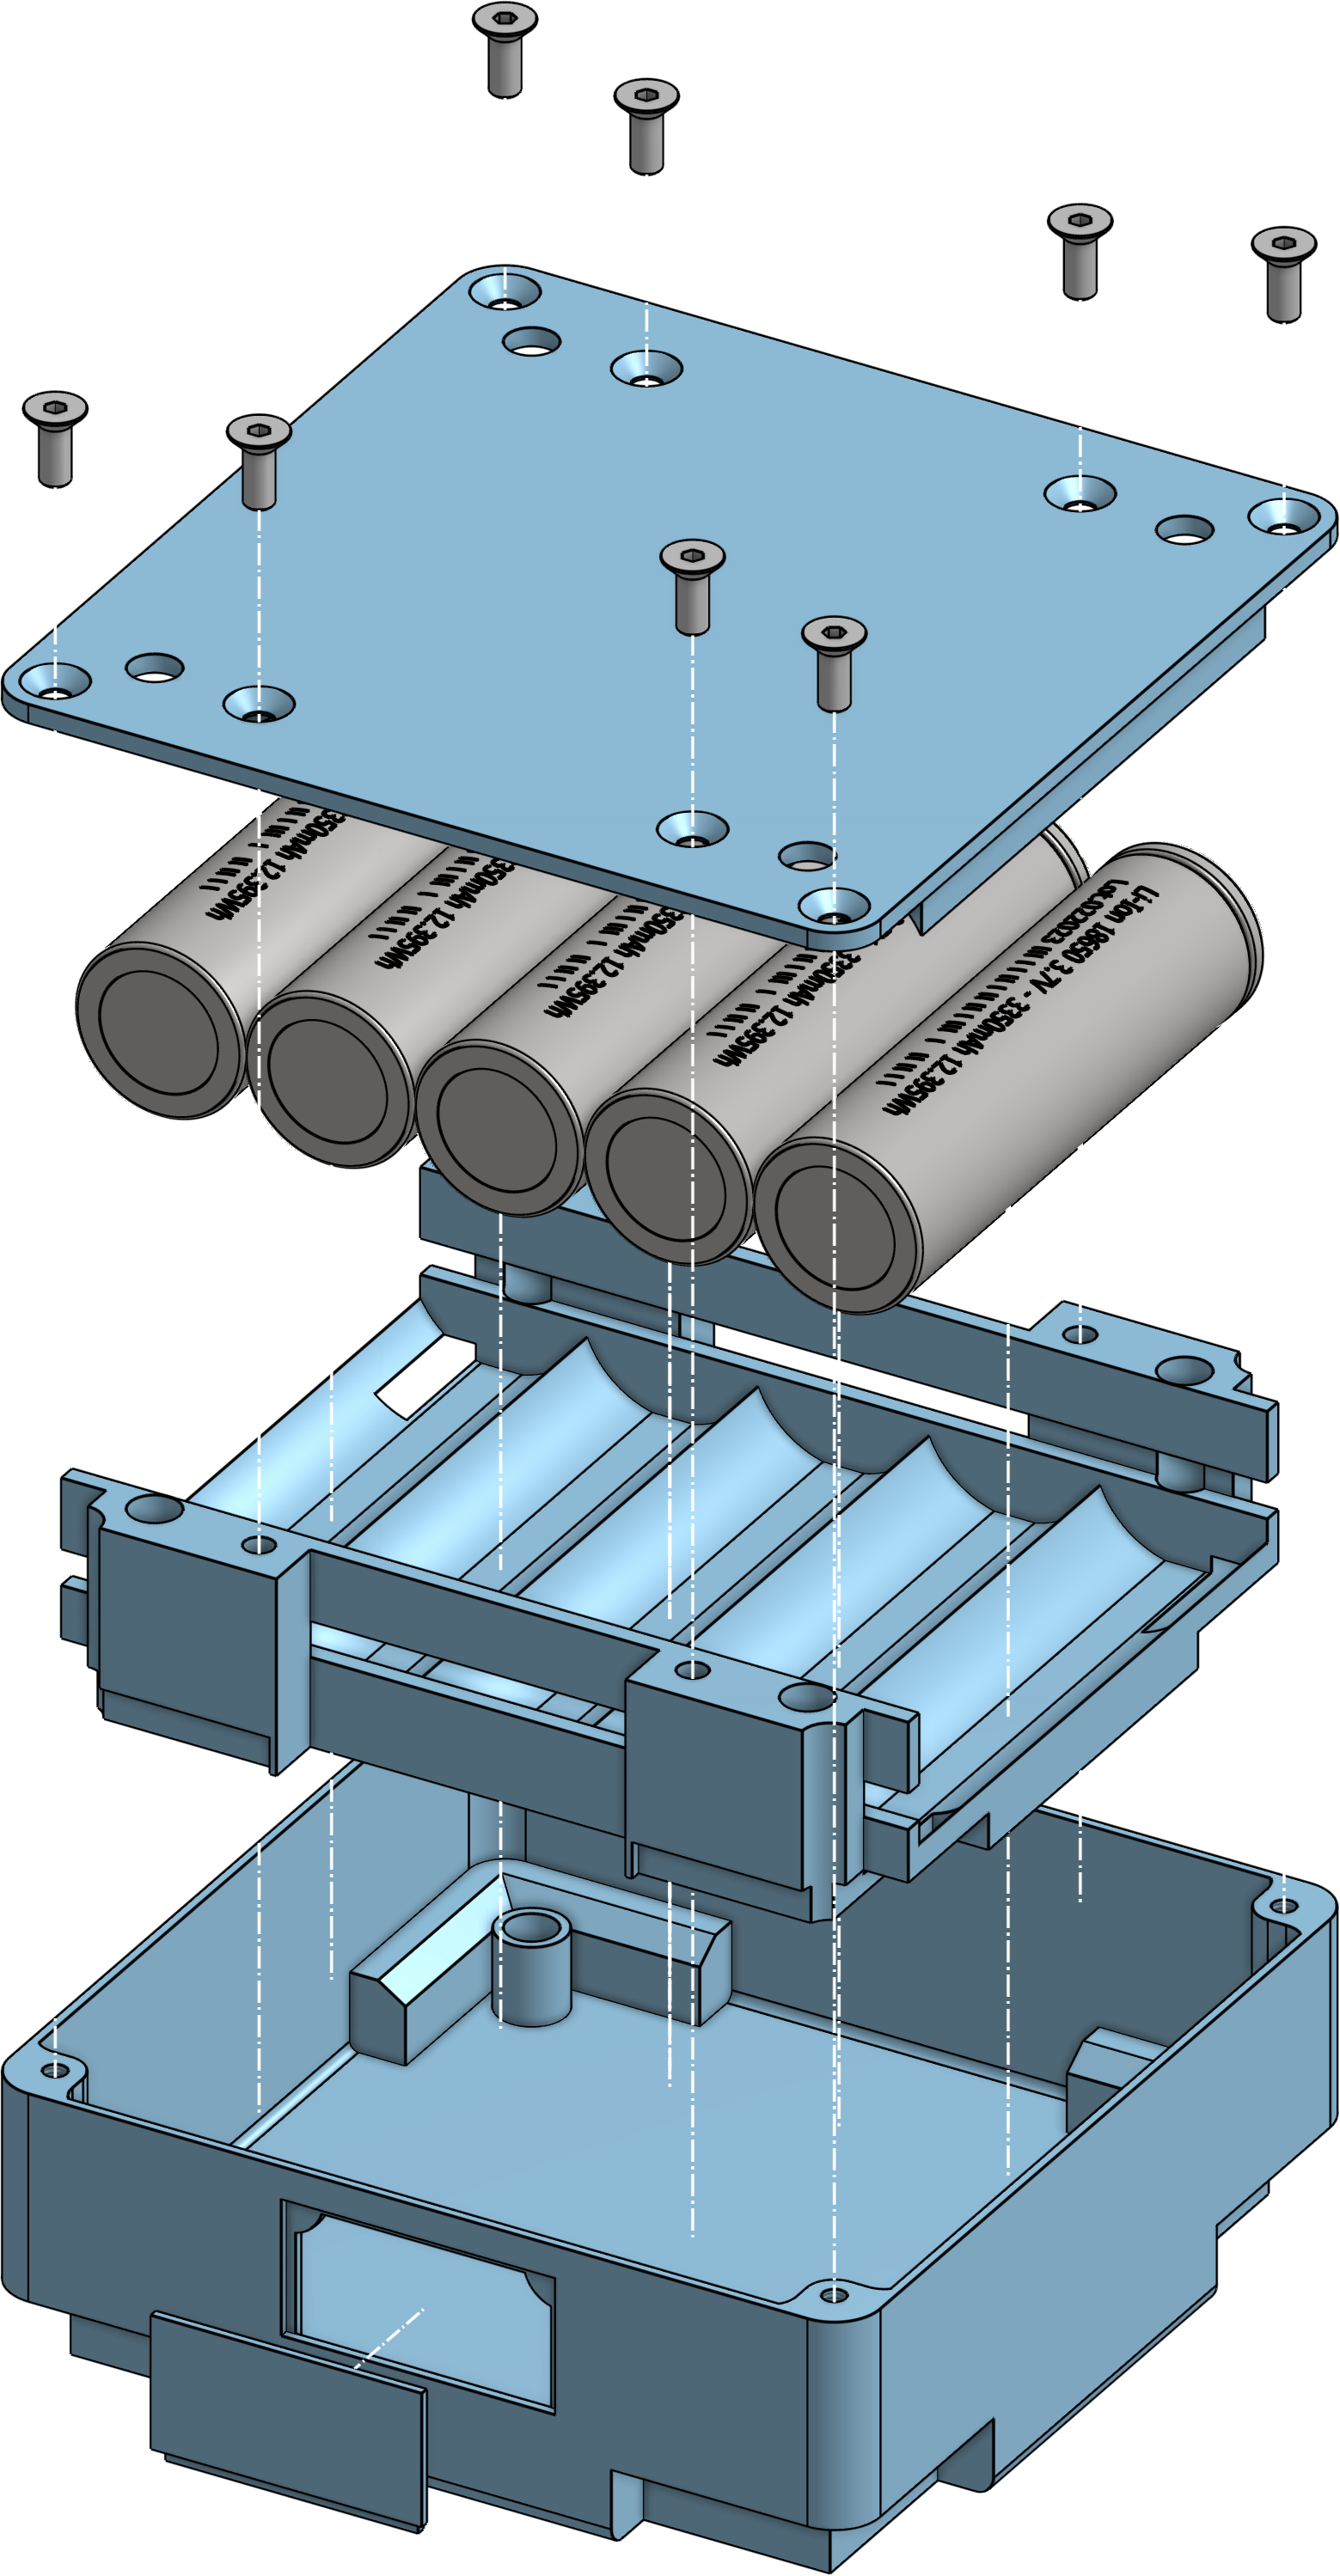
\includegraphics[width=0.3\textwidth]{image/structure/PMS_exploded.png}
        \caption{Vista explotada del \acrshort{pms}.}
      \end{wrapfigure}

      El \acrshort{pms} alberga la batería y la placa del mismo. Para la batería fue necesario crear un soporte que
      la agarra a la tapa y la mantiene fija en todo momento. El montaje de la placa va a depender de la disposición
      de los elementos de la misma. La limitante es el espacio vertical. Actualmente, la placa con componentes no puede
      medir más de 8.4mm de alto. Si logramos disponer los elementos de tal forma de que se pueda levantar para colocar
      tornillos, se usarán tornillos. Caso contrario, se usarán remaches de plástico fundido. La \acrshort{pms} tiene
      una abertura por la tapa superior por donde saldrán todos los cables que van a la \acrshort{obc} y a la
      \acrshort{pu}. La tapa que tiene en la parte frontal de la carcasa está para tener acceso a los conectores de
      potencia y balanceo de la batería para desconectarla completamente del CubeSat y cargarla externamente. La tapa es
      removible y se fija con imanes Además, hay una abertura por donde se expone el conector del \acrshort{hmi}.

      En la tabla \ref{tab:estructura.bom.pms} se puede ver un listado de los componentes requeridos.
      
      \begin{table}[!ht]
        \centering
        \begin{tabular}{|c|c|}
          \hline
          \textbf{Item} & \textbf{Cantidad} \\ \hline
          Tornillos M3  & 8 \\ \hline
          Celdas 18650  & 5 \\ \hline
          Soporte Celdas& 1 \\ \hline
          Tapa Superior & 1 \\ \hline
          Carcasa       & 1 \\ \hline
        \end{tabular}
        \caption{Lista de materiales del modulo \acrshort{pms}}
        \label{tab:estructura.bom.pms}
      \end{table}

    \subsubsection{Módulo \acrshort{obc}}
      La \acrshort{obc} es la más simple de todas. Es solo una tapa con tornillos. La placa con componentes no puede
      medir más de 8mm de alto, por lo que dependiendo de la disposición de los componentes, se verá si se usan
      tornillos o remaches de plástico derretido. En el diseño falta también la misma ventana por donde van a pasar los
      cables.

      En la tabla \ref{tab:estructura.bom.obc} se puede ver un listado de los componentes requeridos.

      \begin{figure}[H]
        \centering
        \begin{minipage}{0.45\textwidth}
          \centering
          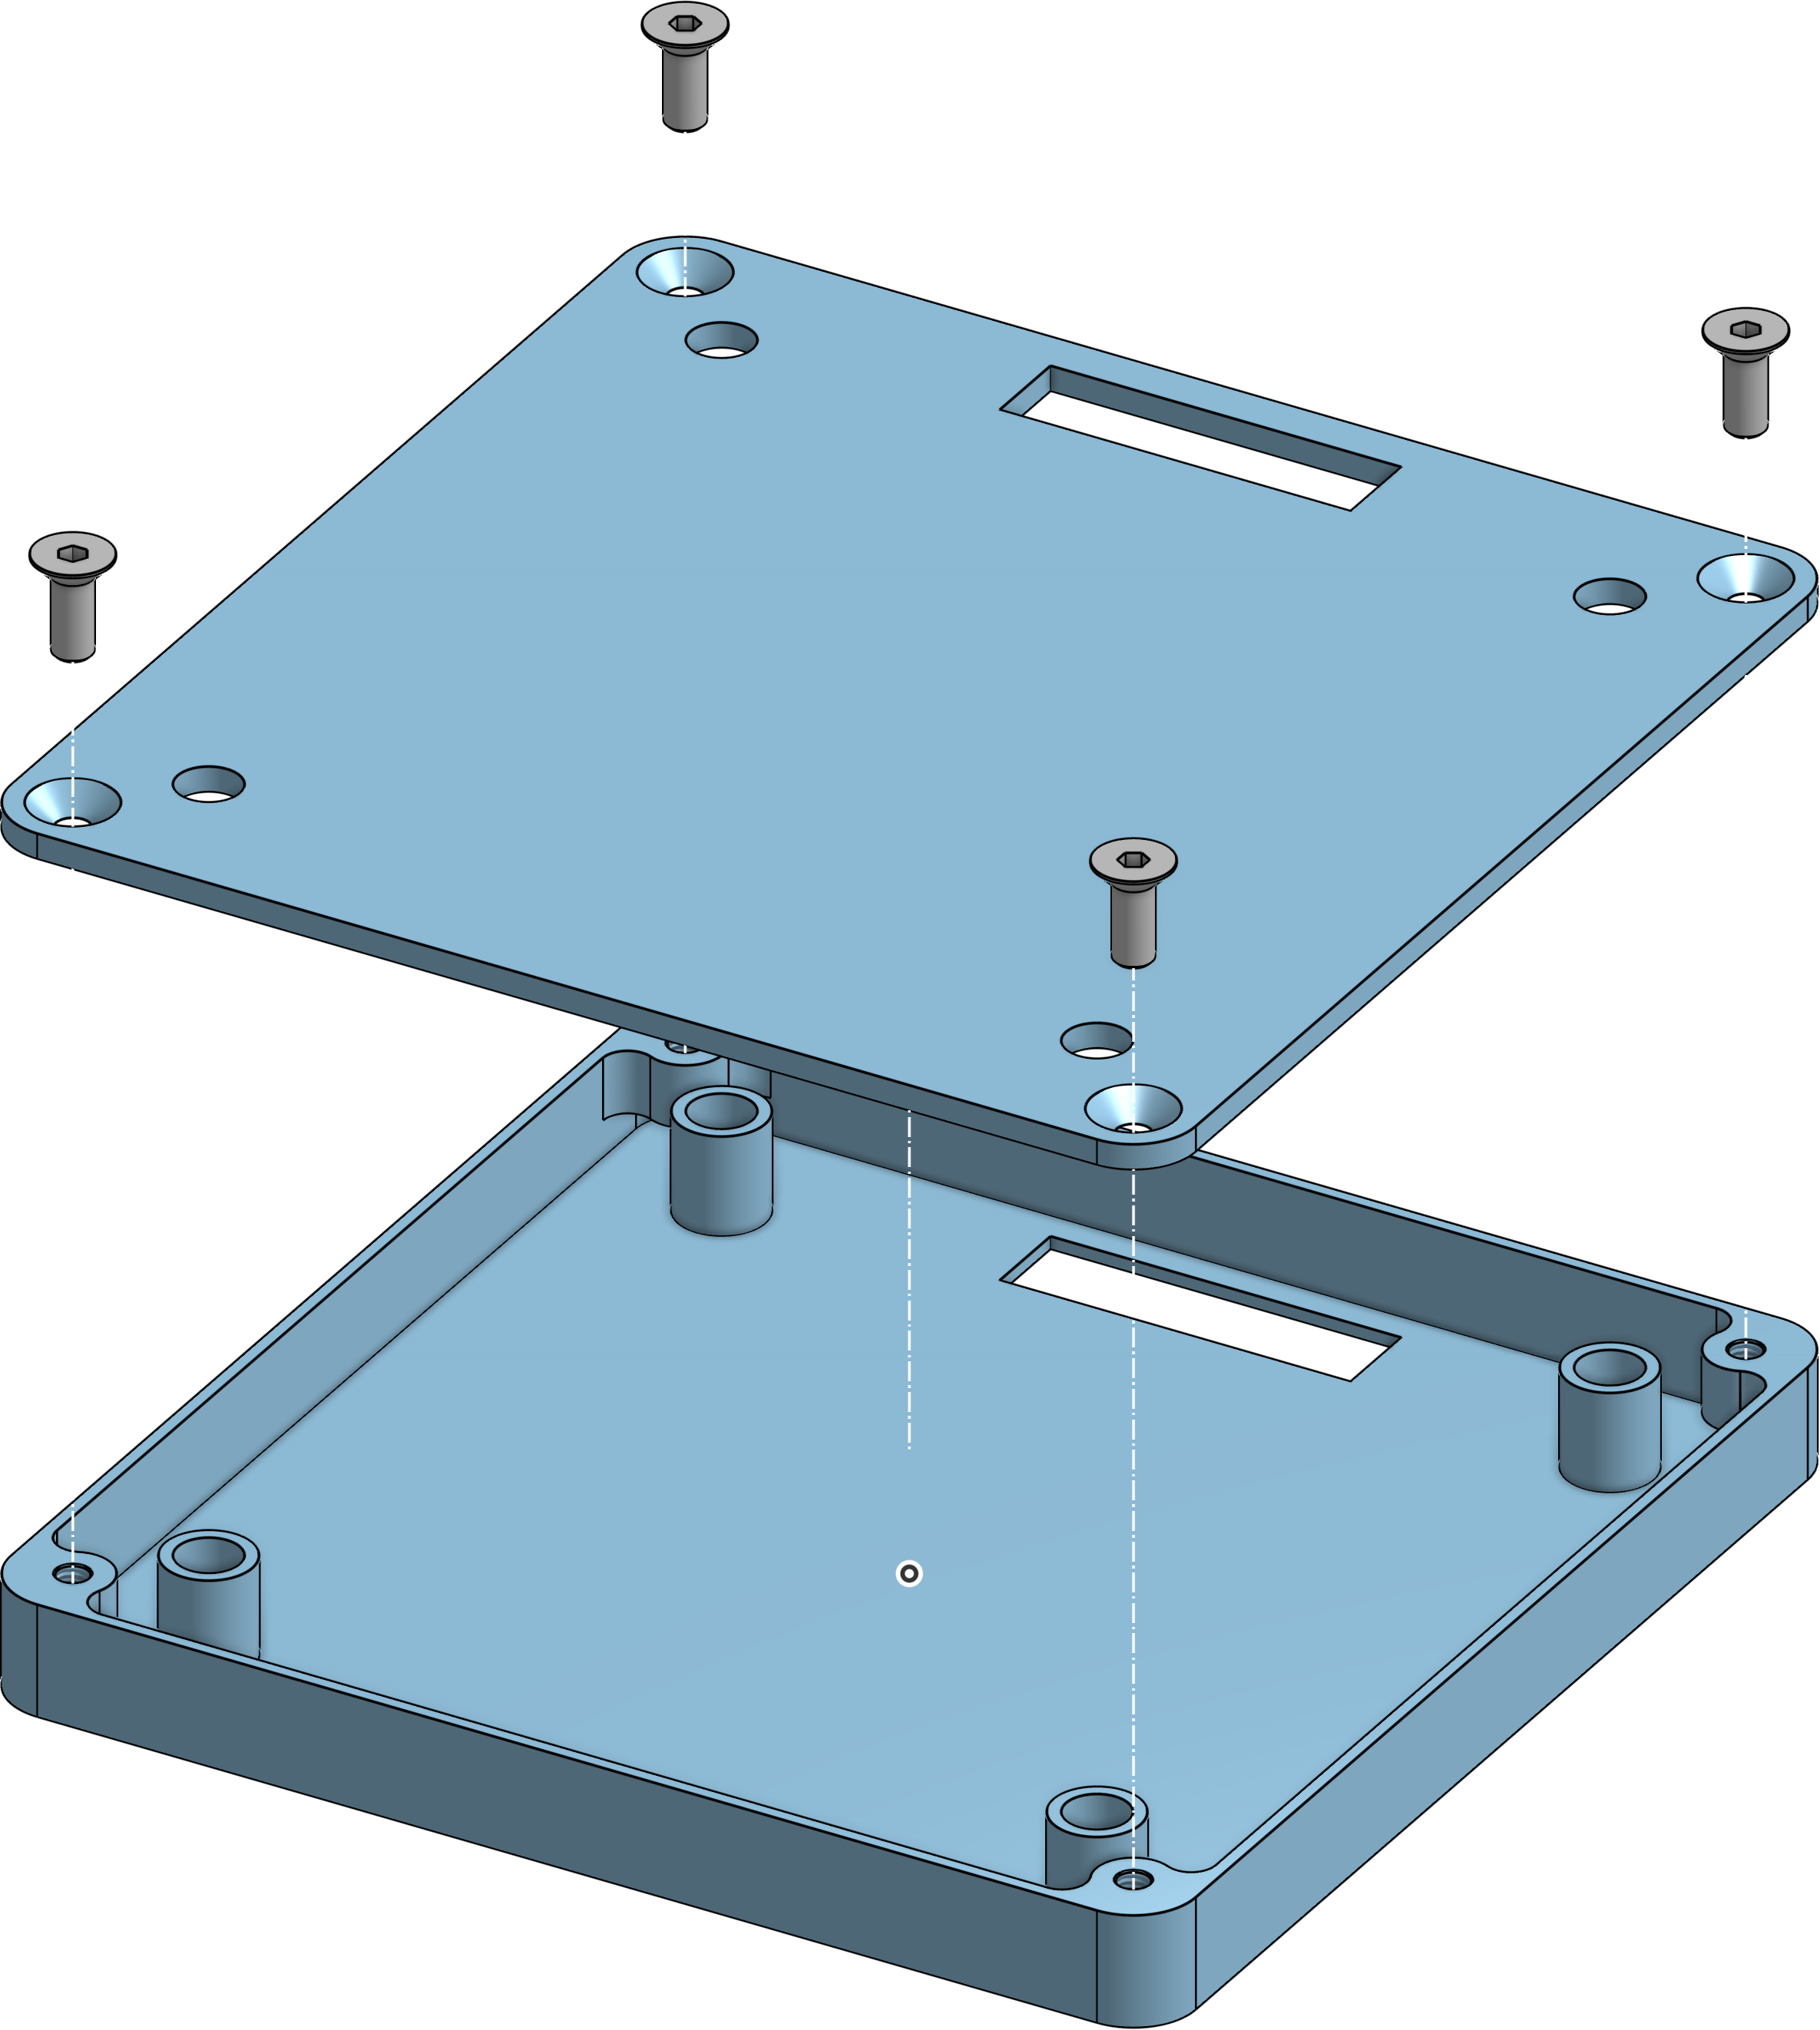
\includegraphics[width=0.5\textwidth]{image/structure/OBC_exploded.png}
          \caption{Vista explotada del \acrshort{obc}.}
        \end{minipage}
        \hfill
        \begin{minipage}{0.45\textwidth}
          \centering
        \begin{tabular}{|c|c|}
          \hline
          \textbf{Item} & \textbf{Cantidad} \\ \hline
          Tornillos M3  & 4 \\ \hline
          Tapa Superior & 1 \\ \hline
          Carcasa       & 1 \\ \hline
        \end{tabular}
          \captionof{table}{Lista de materiales del módulo \acrshort{obc}}
        \label{tab:estructura.bom.obc}
        \end{minipage}
      \end{figure}

    \subsubsection{Módulo \acrshort{pu}}
      \begin{wrapfigure}{l}{0.35\textwidth}
        \centering
        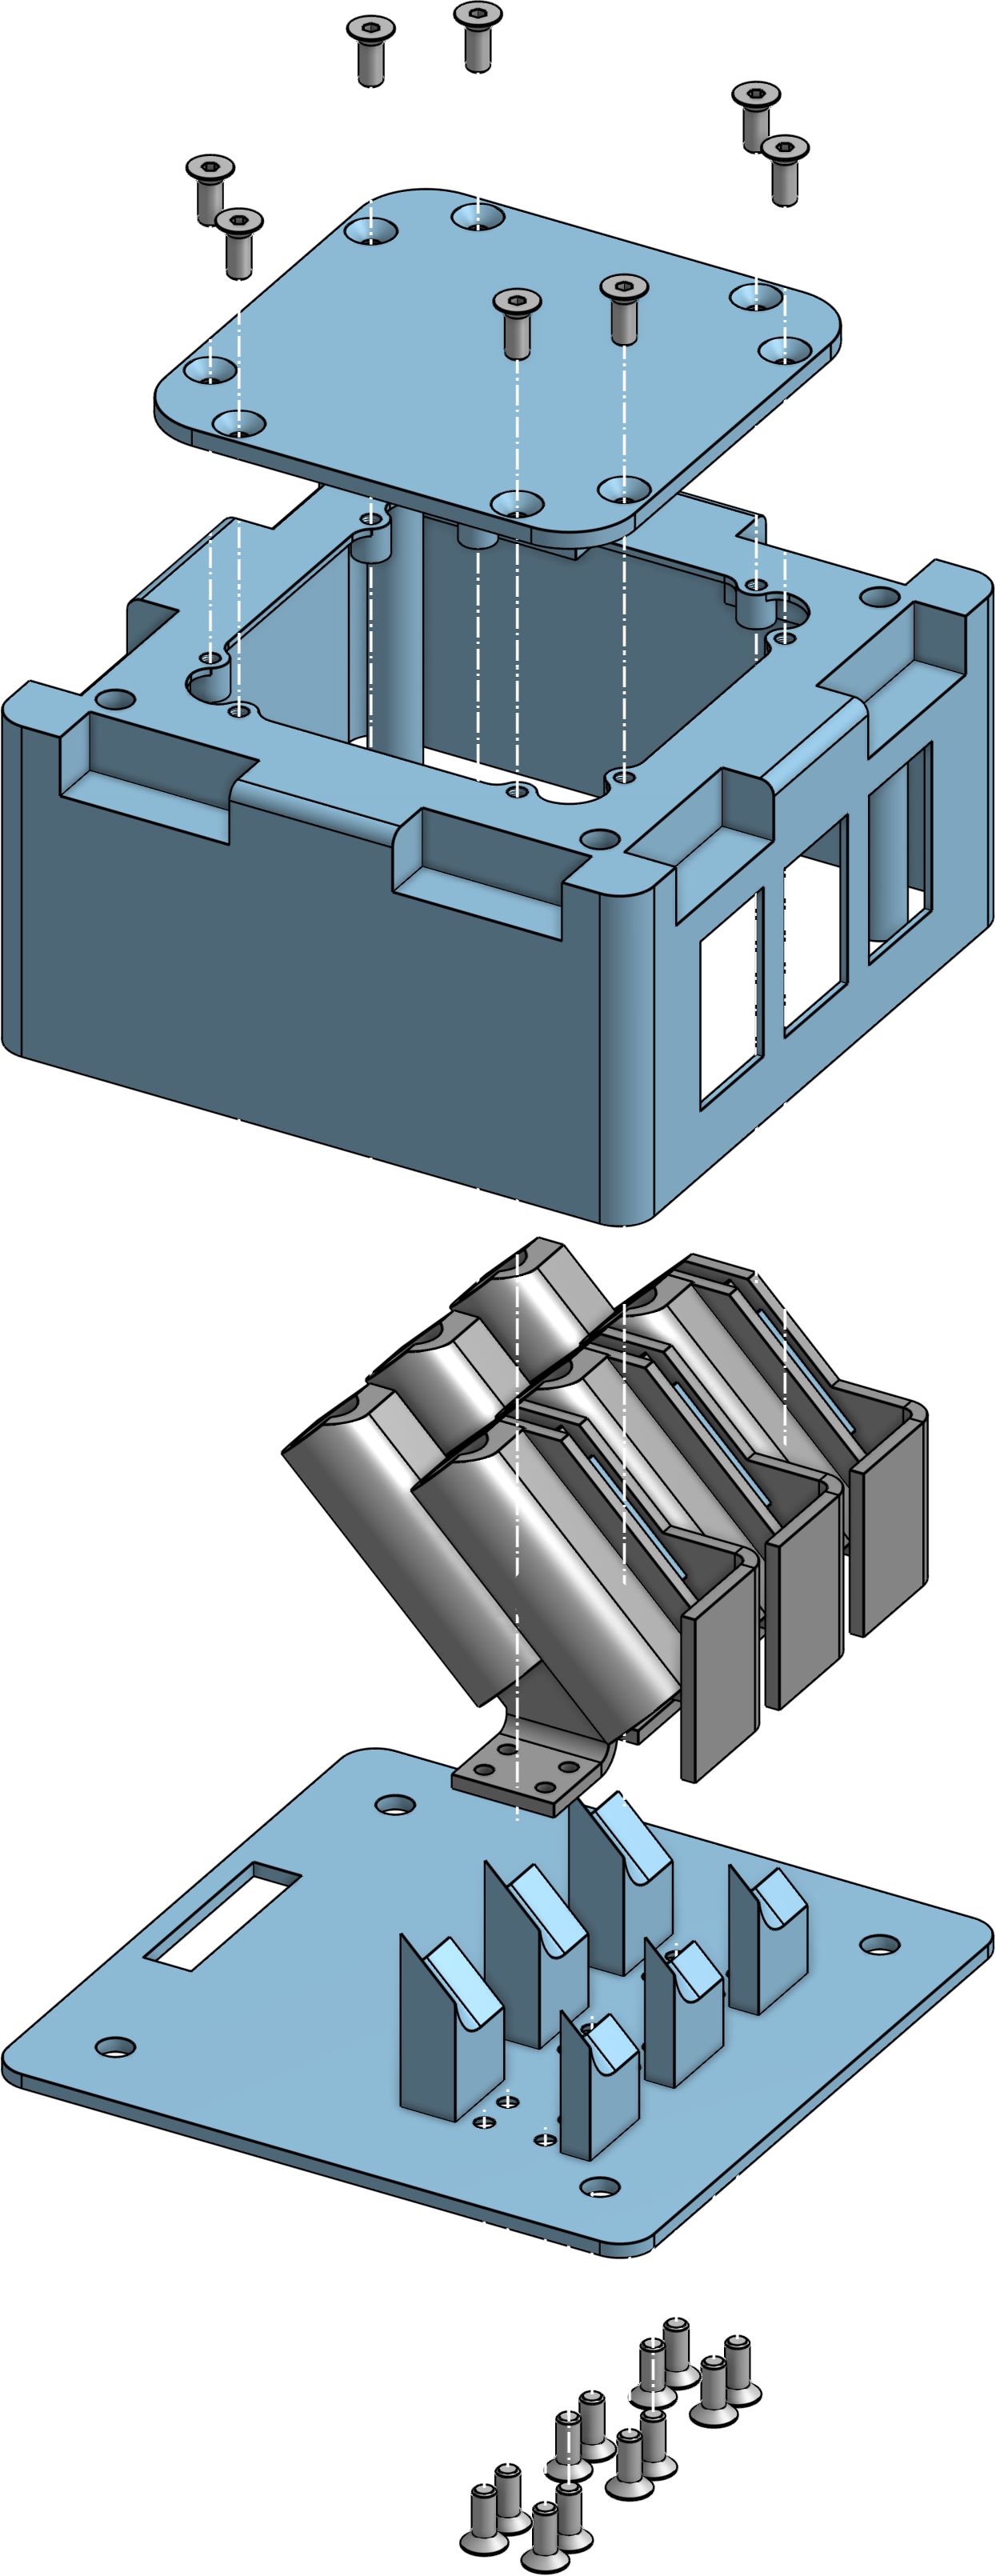
\includegraphics[width=0.3\textwidth]{image/structure/Payload_exploded.png}
        \caption{Vista explotada del Payload Unit.}
      \end{wrapfigure}
      La \acrshort{pu} es el que alberga las tres zonas térmicas reguladas, las de cuáles cada una alberga dos muestras.
      Este subsistema es el único que no tiene placa. La \acrshort{pu} tiene una tapa superior, que como se mencionó
      previamente, es por la cual se cargaran las muestras en el momento previo a cargar el CubeSat al cohete. Por otro
      lado, la carcasa tiene tres aberturas las cuales son para exponer una chapa que está en contacto con las Peltier
      de cada zona térmica. Esta chapa, por el momento, va a estar al ras de la carcasa, para aportar disipación para
      las celdas Peltier. Está planeado determinar de forma experimental si se requiere aumentar la superficie de
      disipación (agregando por ejemplo un disipador) o es necesario emplear un sistema de disipación activo.
      Decidimos hacer pruebas experimentales, ya que no conocemos con exactitud cuál va a ser la demanda para llevar cada
      bloque y las muestras a la temperatura deseada. Además, es posible que durante el periodo de estabilización térmica
      la solución de disipación no sea suficiente, pero una vez estabilizado si lo sea. Como planeamos que la
      estabilización térmica ocurra bajo la supervisión del equipo, no sería necesario cambiar el sistema de
      disipación.

      Cada zona térmica regulada está compuesta por una chapa plegada, perforada y mecanizada, a la cual se le agregan 4
      separadores plásticos pegados con pegamento epoxico. A esa pieza que llamamos "Mount" se le coloca el bloque
      mecanizado de aluminio que albergará los tubos de plástico donde se colocarán las muestras. La forma en la que él
      bloque mecanizado se unirá al mount aún no está definida. Dentro de las opciones están: Soldadura aditiva (mig,
      tig o con estaño), pegamento epoxico térmico, o silicona térmica. Se prefiere las soldaduras aditivas por su
      mejor conducción térmica. Además, al mount se le coloca la Celda Peltier (con pasta térmica de ambos lados), la
      cuál es fijada por otra chapa de aluminio plegada, perforada y mecanizada, la cual es la principal forma de
      disipación para la celda Peltier. La parte plegada de la chapa de transferencia térmica queda expuesta al exterior
      por medio de una ventana en la carcasa de la Payload Unit.

      En la tabla \ref{tab:estructura.bom.pu} se puede ver un listado de los componentes requeridos.
      \begin{figure}[!ht]
        \centering
        \begin{minipage}{0.35\textwidth}
          \centering
          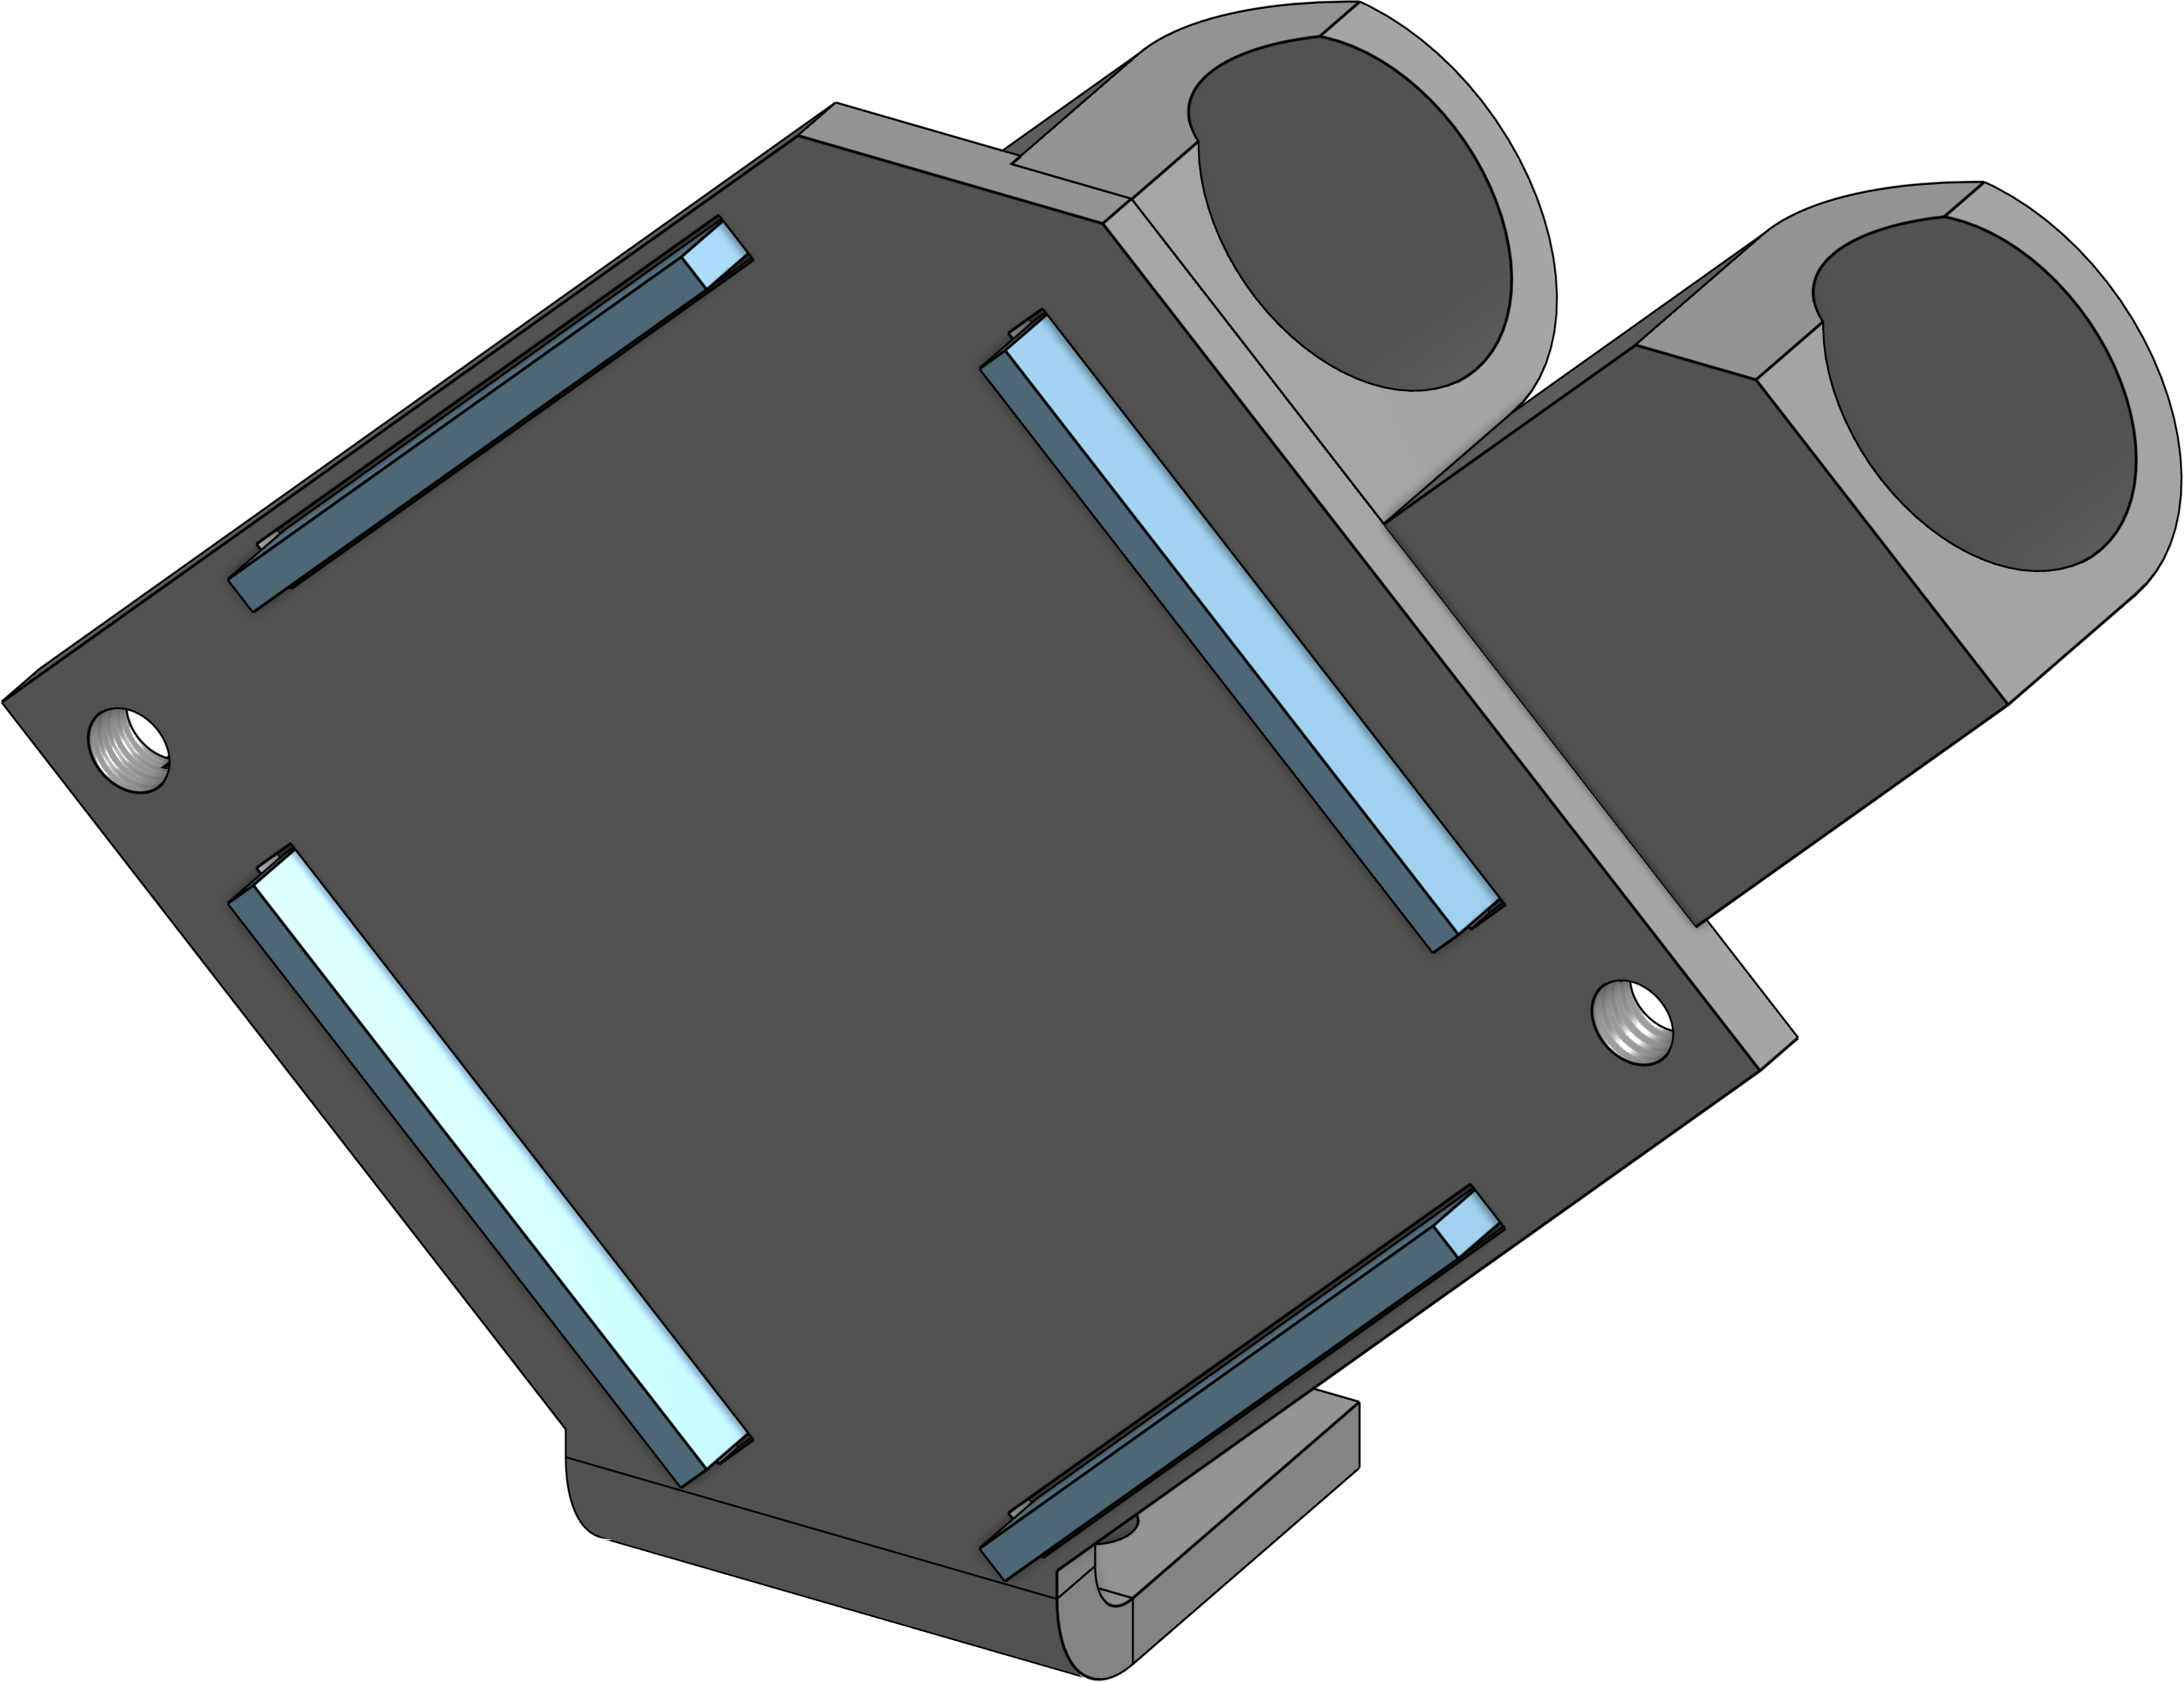
\includegraphics[width=1\textwidth]{image/structure/SampleUnit.png}
        \end{minipage}
        \hfill
        \begin{minipage}{0.45\textwidth}
          \centering
          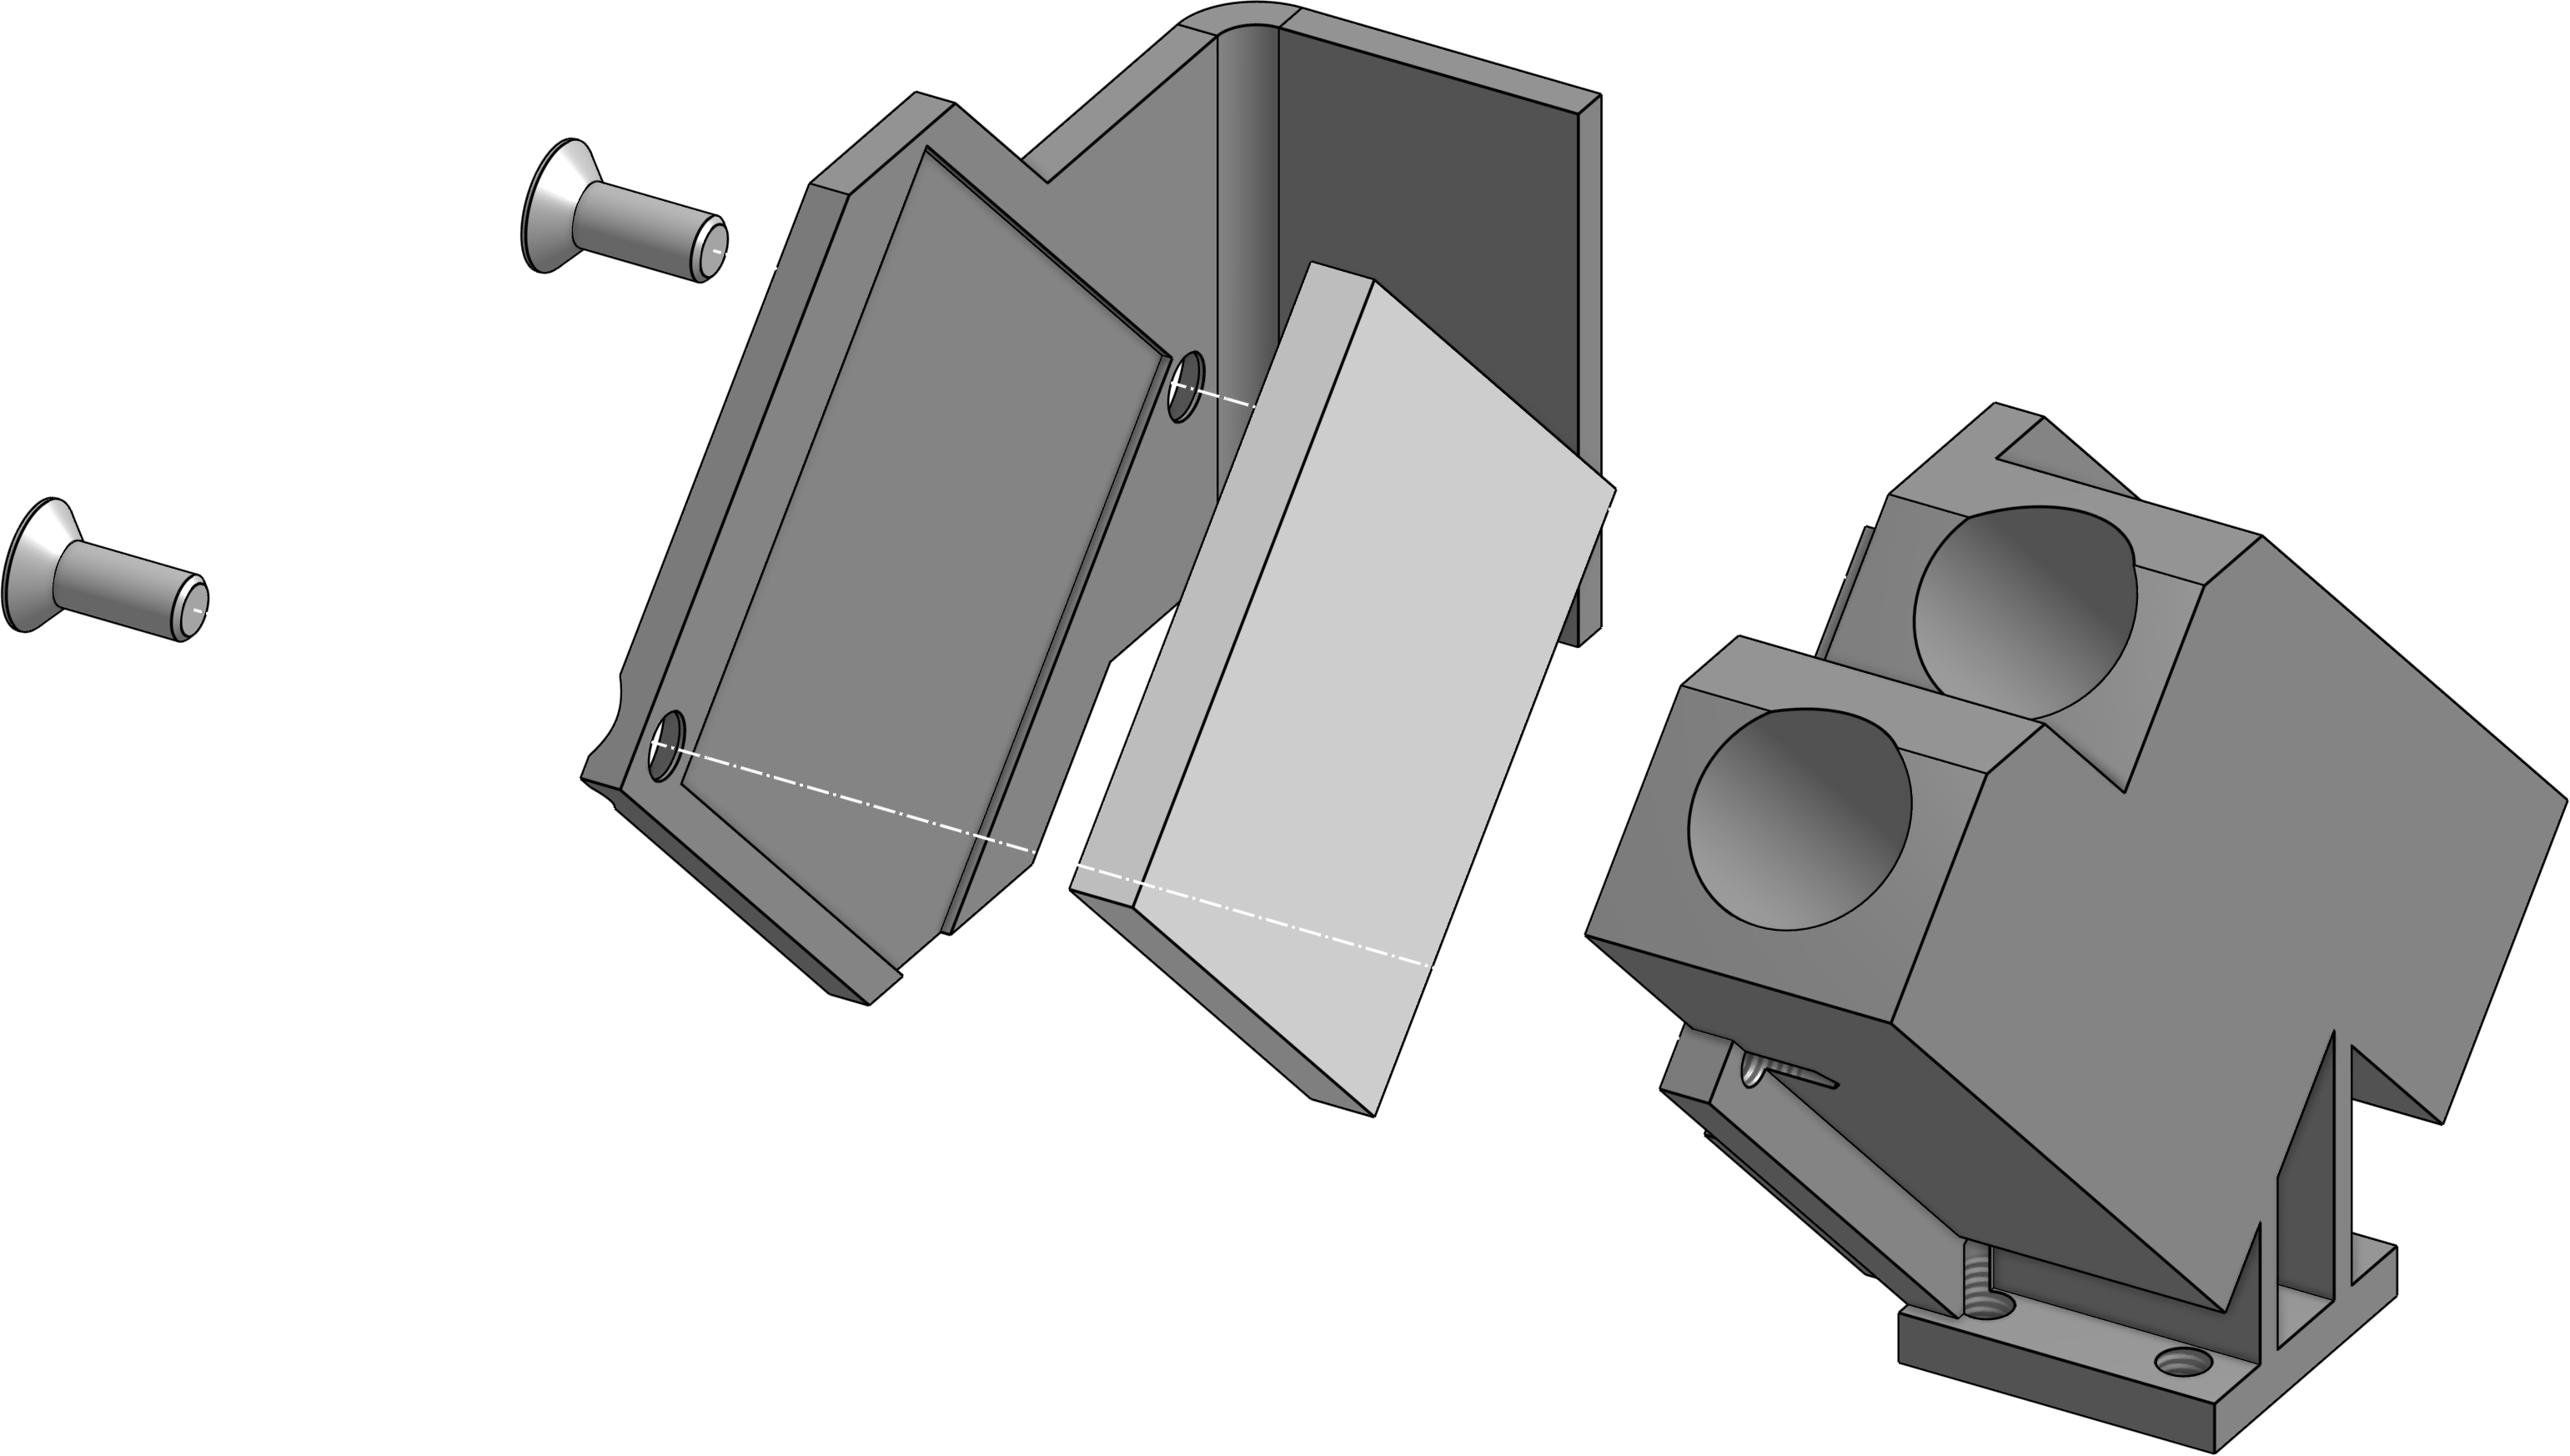
\includegraphics[width=1\textwidth]{image/structure/SampleUnit_exploded.png}
        \end{minipage}
        \caption{Vistas varias de la zona térmica regulada.}
      \end{figure}

      \begin{table}[!ht]
        \centering
        \begin{tabular}{|c|c|}
          \hline
          \textbf{Item}     & \textbf{Cantidad} \\ \hline
          Tornillos M3      & 24 \\ \hline
          Celdas Peltier    & 3 \\ \hline
          Chapa Disipadora  & 3 \\ \hline
          Bloque de muestras& 3 \\ \hline
          Mount             & 3 \\ \hline
          Tapa superior     & 1 \\ \hline
          Tapa inferior     & 1 \\ \hline
          Carcasa           & 1 \\ \hline
        \end{tabular}
        \caption{Lista de materiales del modulo \acrshort{pms}}
        \label{tab:estructura.bom.pu}
      \end{table}

    \subsubsection{Fabricación}
      Para la fabricación del CubeSat, solamente se requiere una plancha de aluminio como materia prima para obtener él
      esqueleto básico del mismo. La plancha de aluminio debe ser cortada previo al plegado, ya que algunos cortes
      implementan geometrías que no solo facilitan los pliegues, sino que en algunos casos los hacen posibles,
      agregando puntos de alivio. Además de los cortes, es necesario hacer las marcas de centro para las perforaciones
      necesarias, ya que hacer los agujeros en tamaño completo puede provocar deformaciones en los mismos al momento del
      plegado.
      \begin{figure}[H]
        \begin{minipage}{0.5\textwidth}
          \centering
          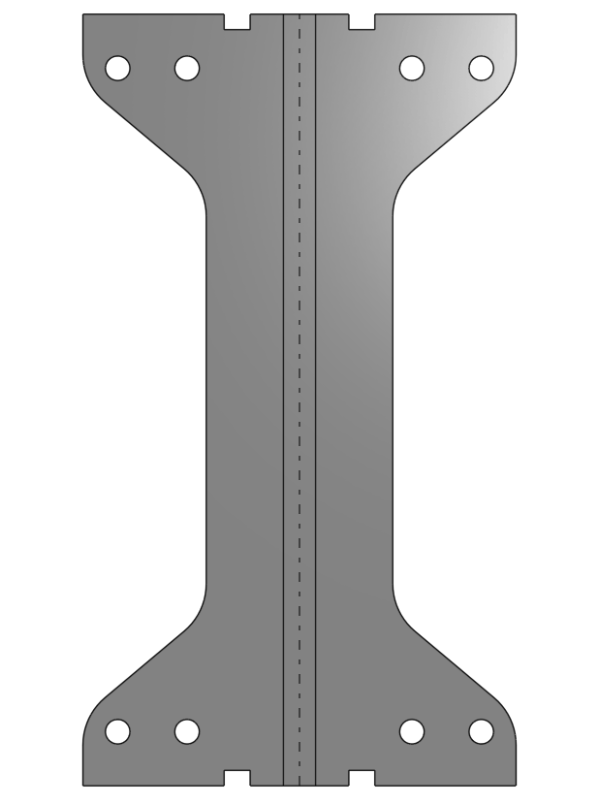
\includegraphics[width=50mm]{image/structure/cornerFlat.png}
          \caption{Corner previo al plegado}
          \label{fig:cornerfp}
        \end{minipage}
        \begin{minipage}{0.5\textwidth}
          \centering
          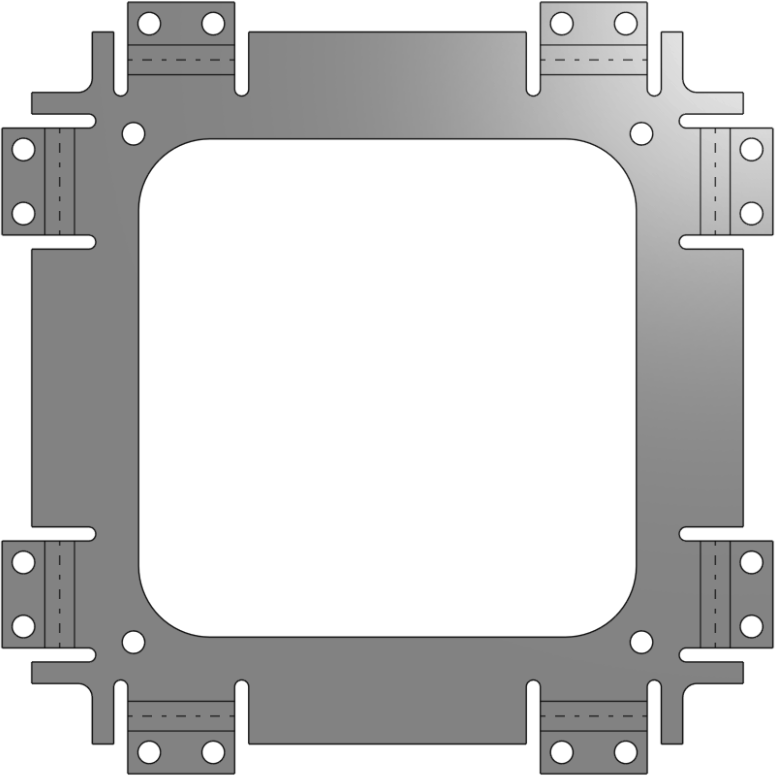
\includegraphics[width=50mm]{image/structure/lidFlat.png}
          \caption{Lid previo al plegado}
          \label{fig:lidfp}
        \end{minipage}
      \end{figure}

      Para realizar los cortes de la plancha de aluminio se utilizará la CNC disponible en el Centro de Investigación
      en Informática para la Ingeniería (CIII). Luego de los cortes, se quitan las rebabas utilizando herramientas
      manuales, y se procede al plegado.

      Para el plegado, especialmente el plegado de los Lid, se requiere maquinaria especializada de plegado, que es poco
      frecuente y su uso aumentaría significativamente el costo de fabricación del CubeSat. Por eso, se diseñaron unas
      matrices y punzones para ser impresos en 3D con PLA y relleno al 100\% y utilizados en una morsa de banco. Esto
      permite que tengamos control total sobre los pliegues, radios y tensiones generadas en las chapas al momento del
      plegado.

      En las figuras \ref{fig:fabricacion.lid} y \ref{fig:fabricacion.corner} se pueden ver las herramientas que
      diseñamos y como quedan después de hacer el pliegue. Seguimos desarrollando herramientas que permitan tener más
      control sobre la línea de pliegue, pero ya fuimos capaces de crear un primer prototipo que se puede ver en la
      figura \ref{fig:fabricacion.prototipo1}.
      \begin{figure}[!ht]
        \centering
        \begin{minipage}{.32\textwidth}
          \centering
          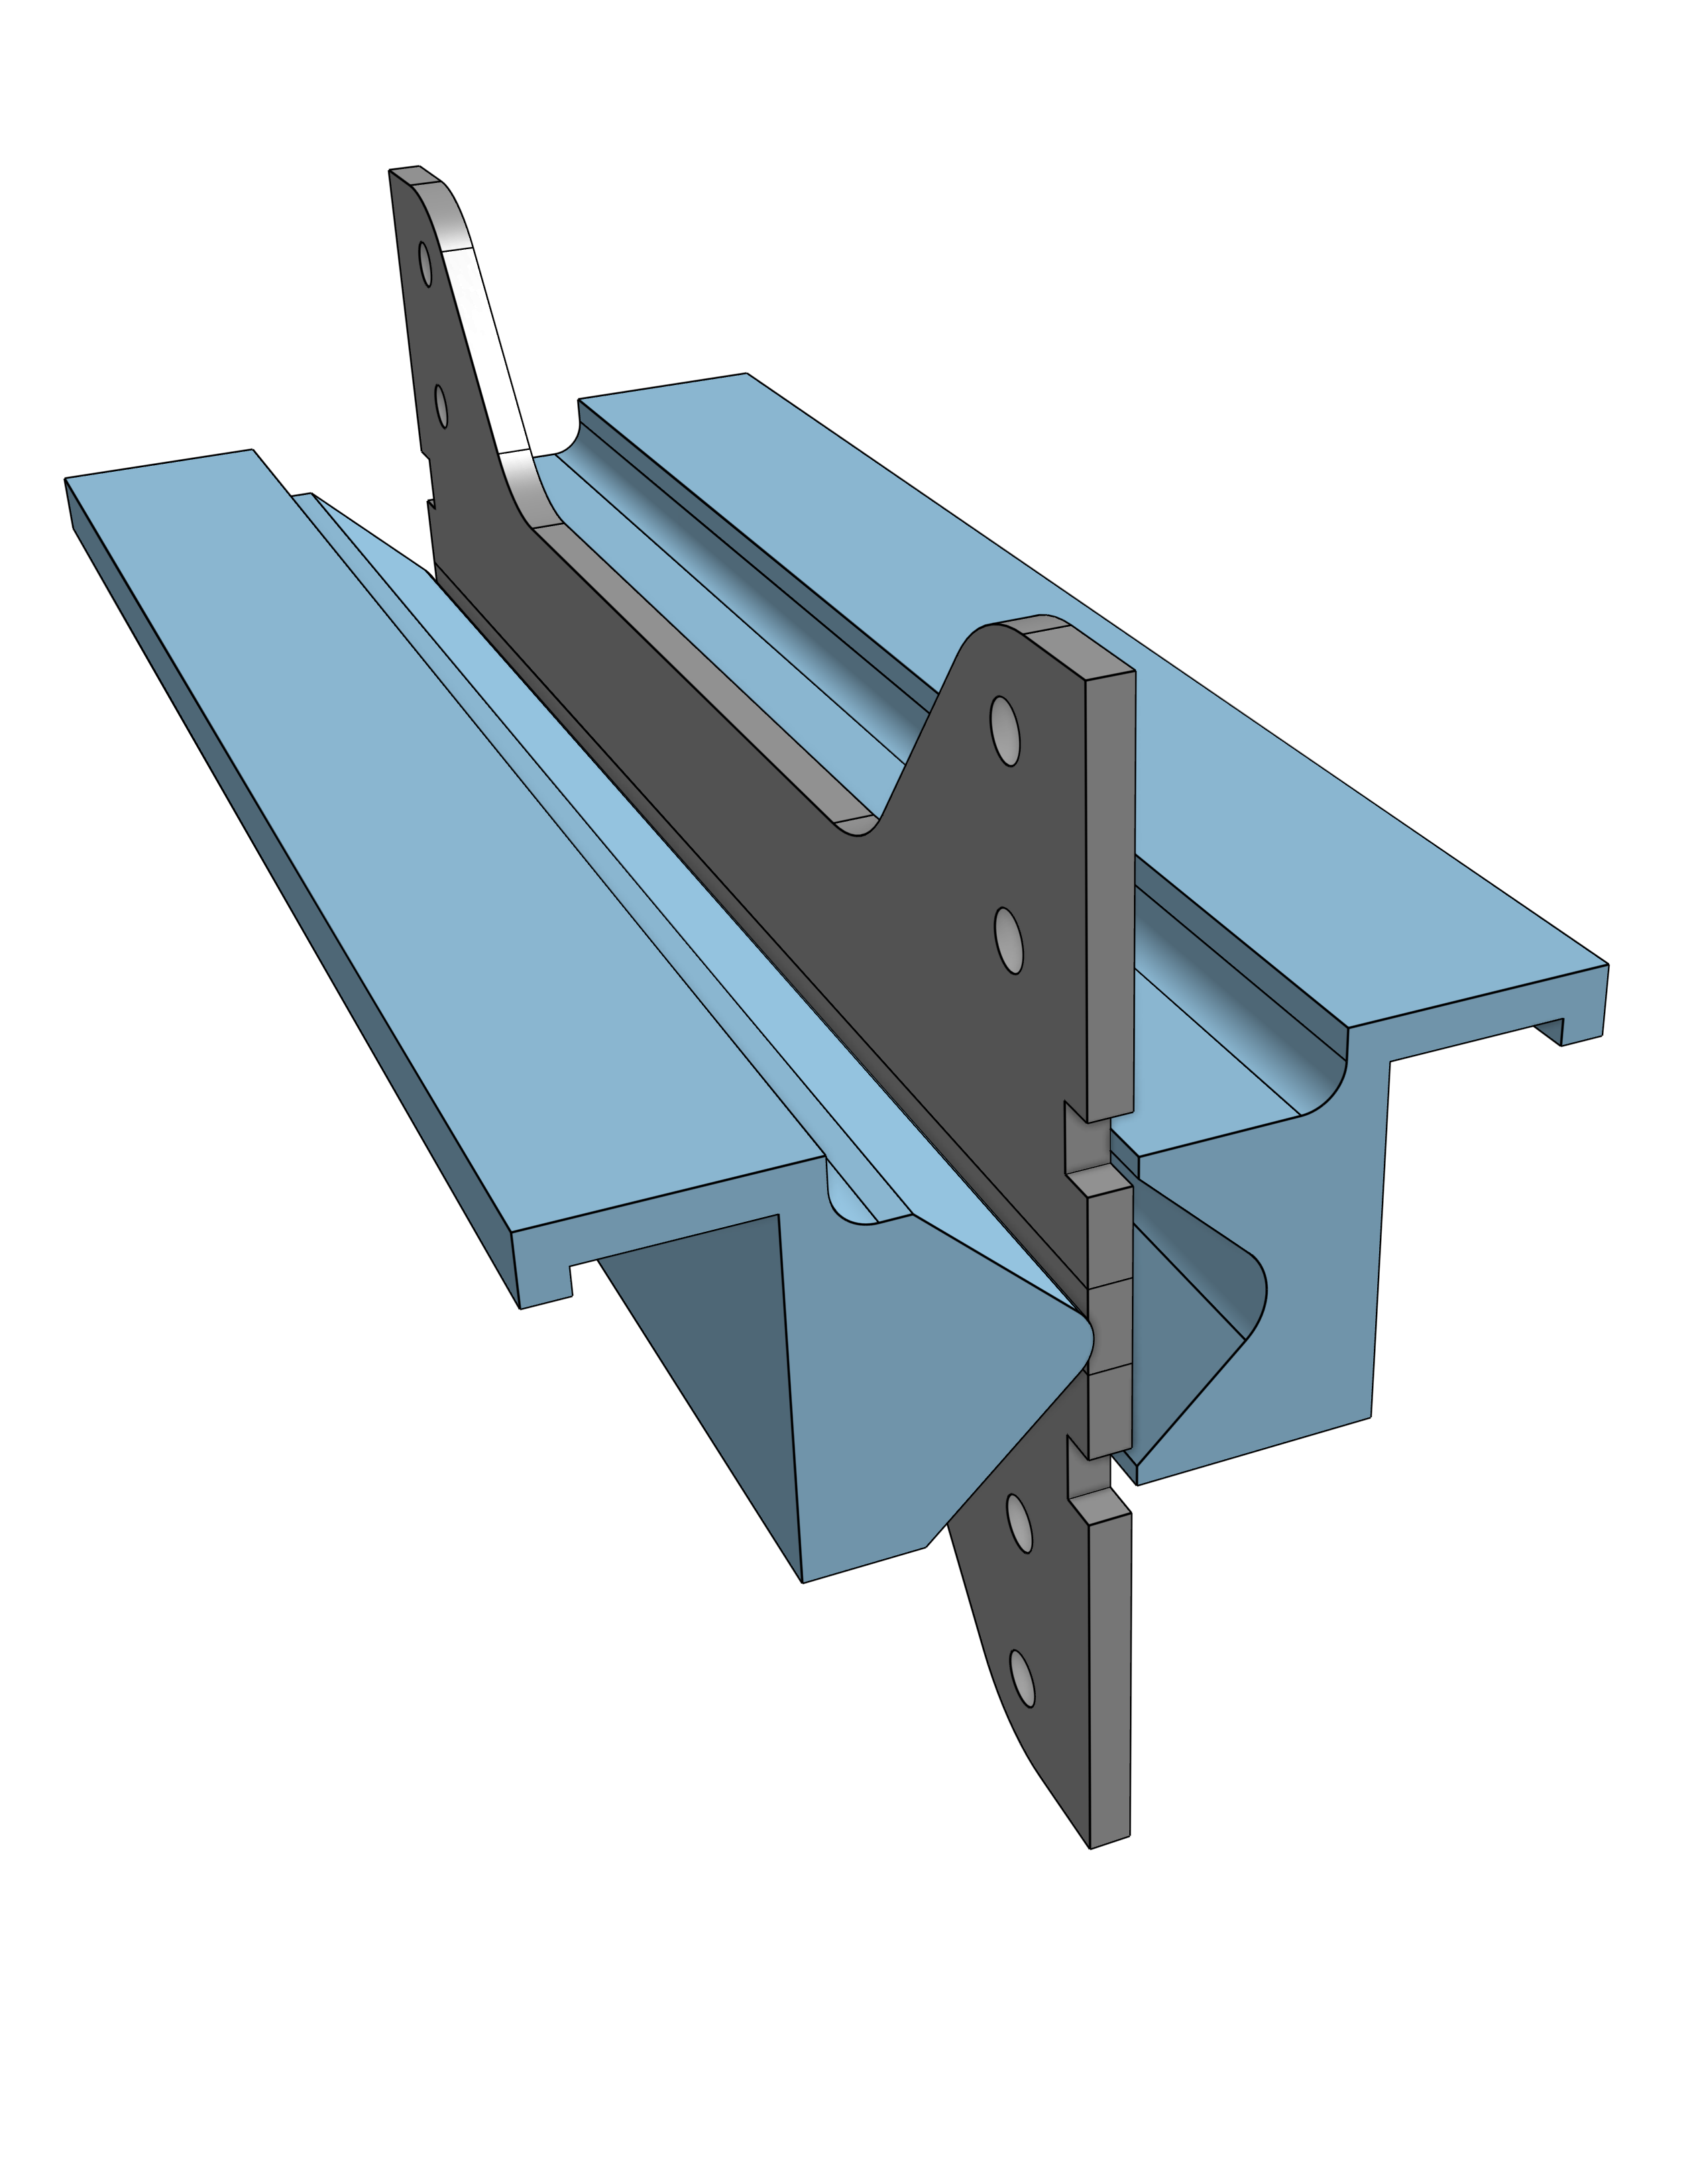
\includegraphics[width=\textwidth]{image/fabrication/corner_flat_top.png}
        \end{minipage}
        \hfill
        \begin{minipage}{.32\textwidth}
          \centering
          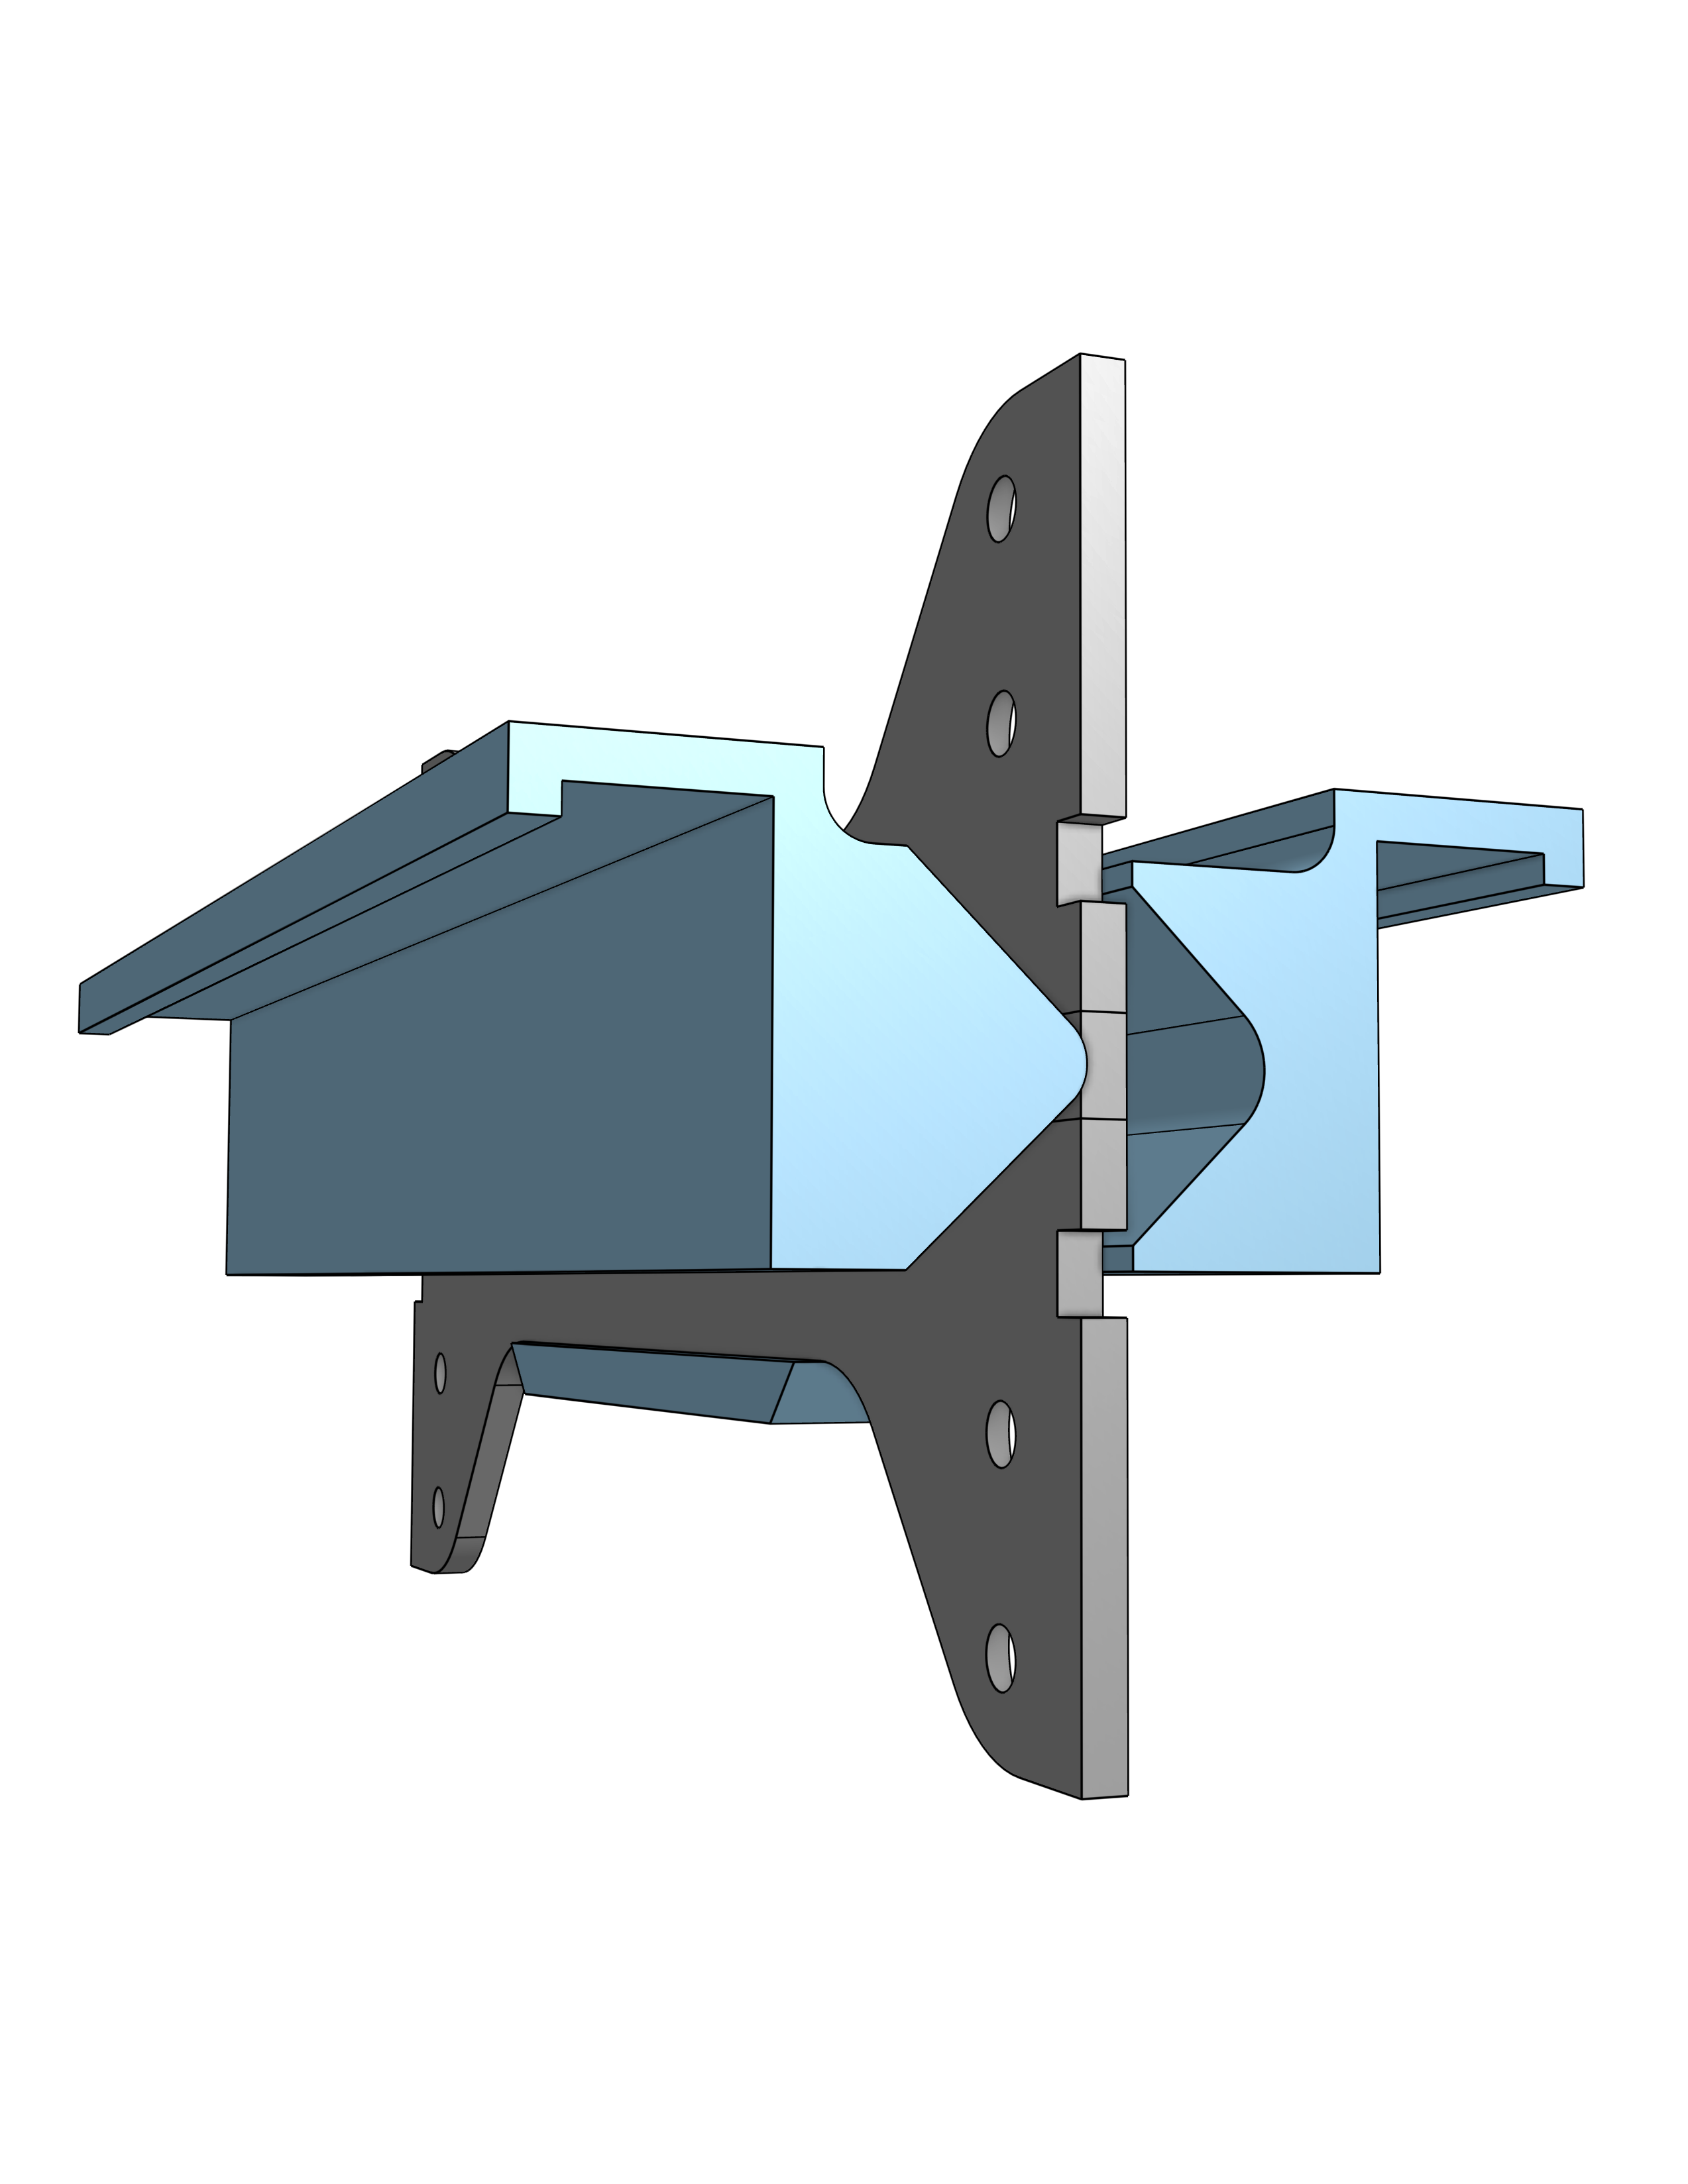
\includegraphics[width=\textwidth]{image/fabrication/corner_flat_bottom.png}
        \end{minipage}
        \hfill
        \begin{minipage}{.32\textwidth}
          \centering
          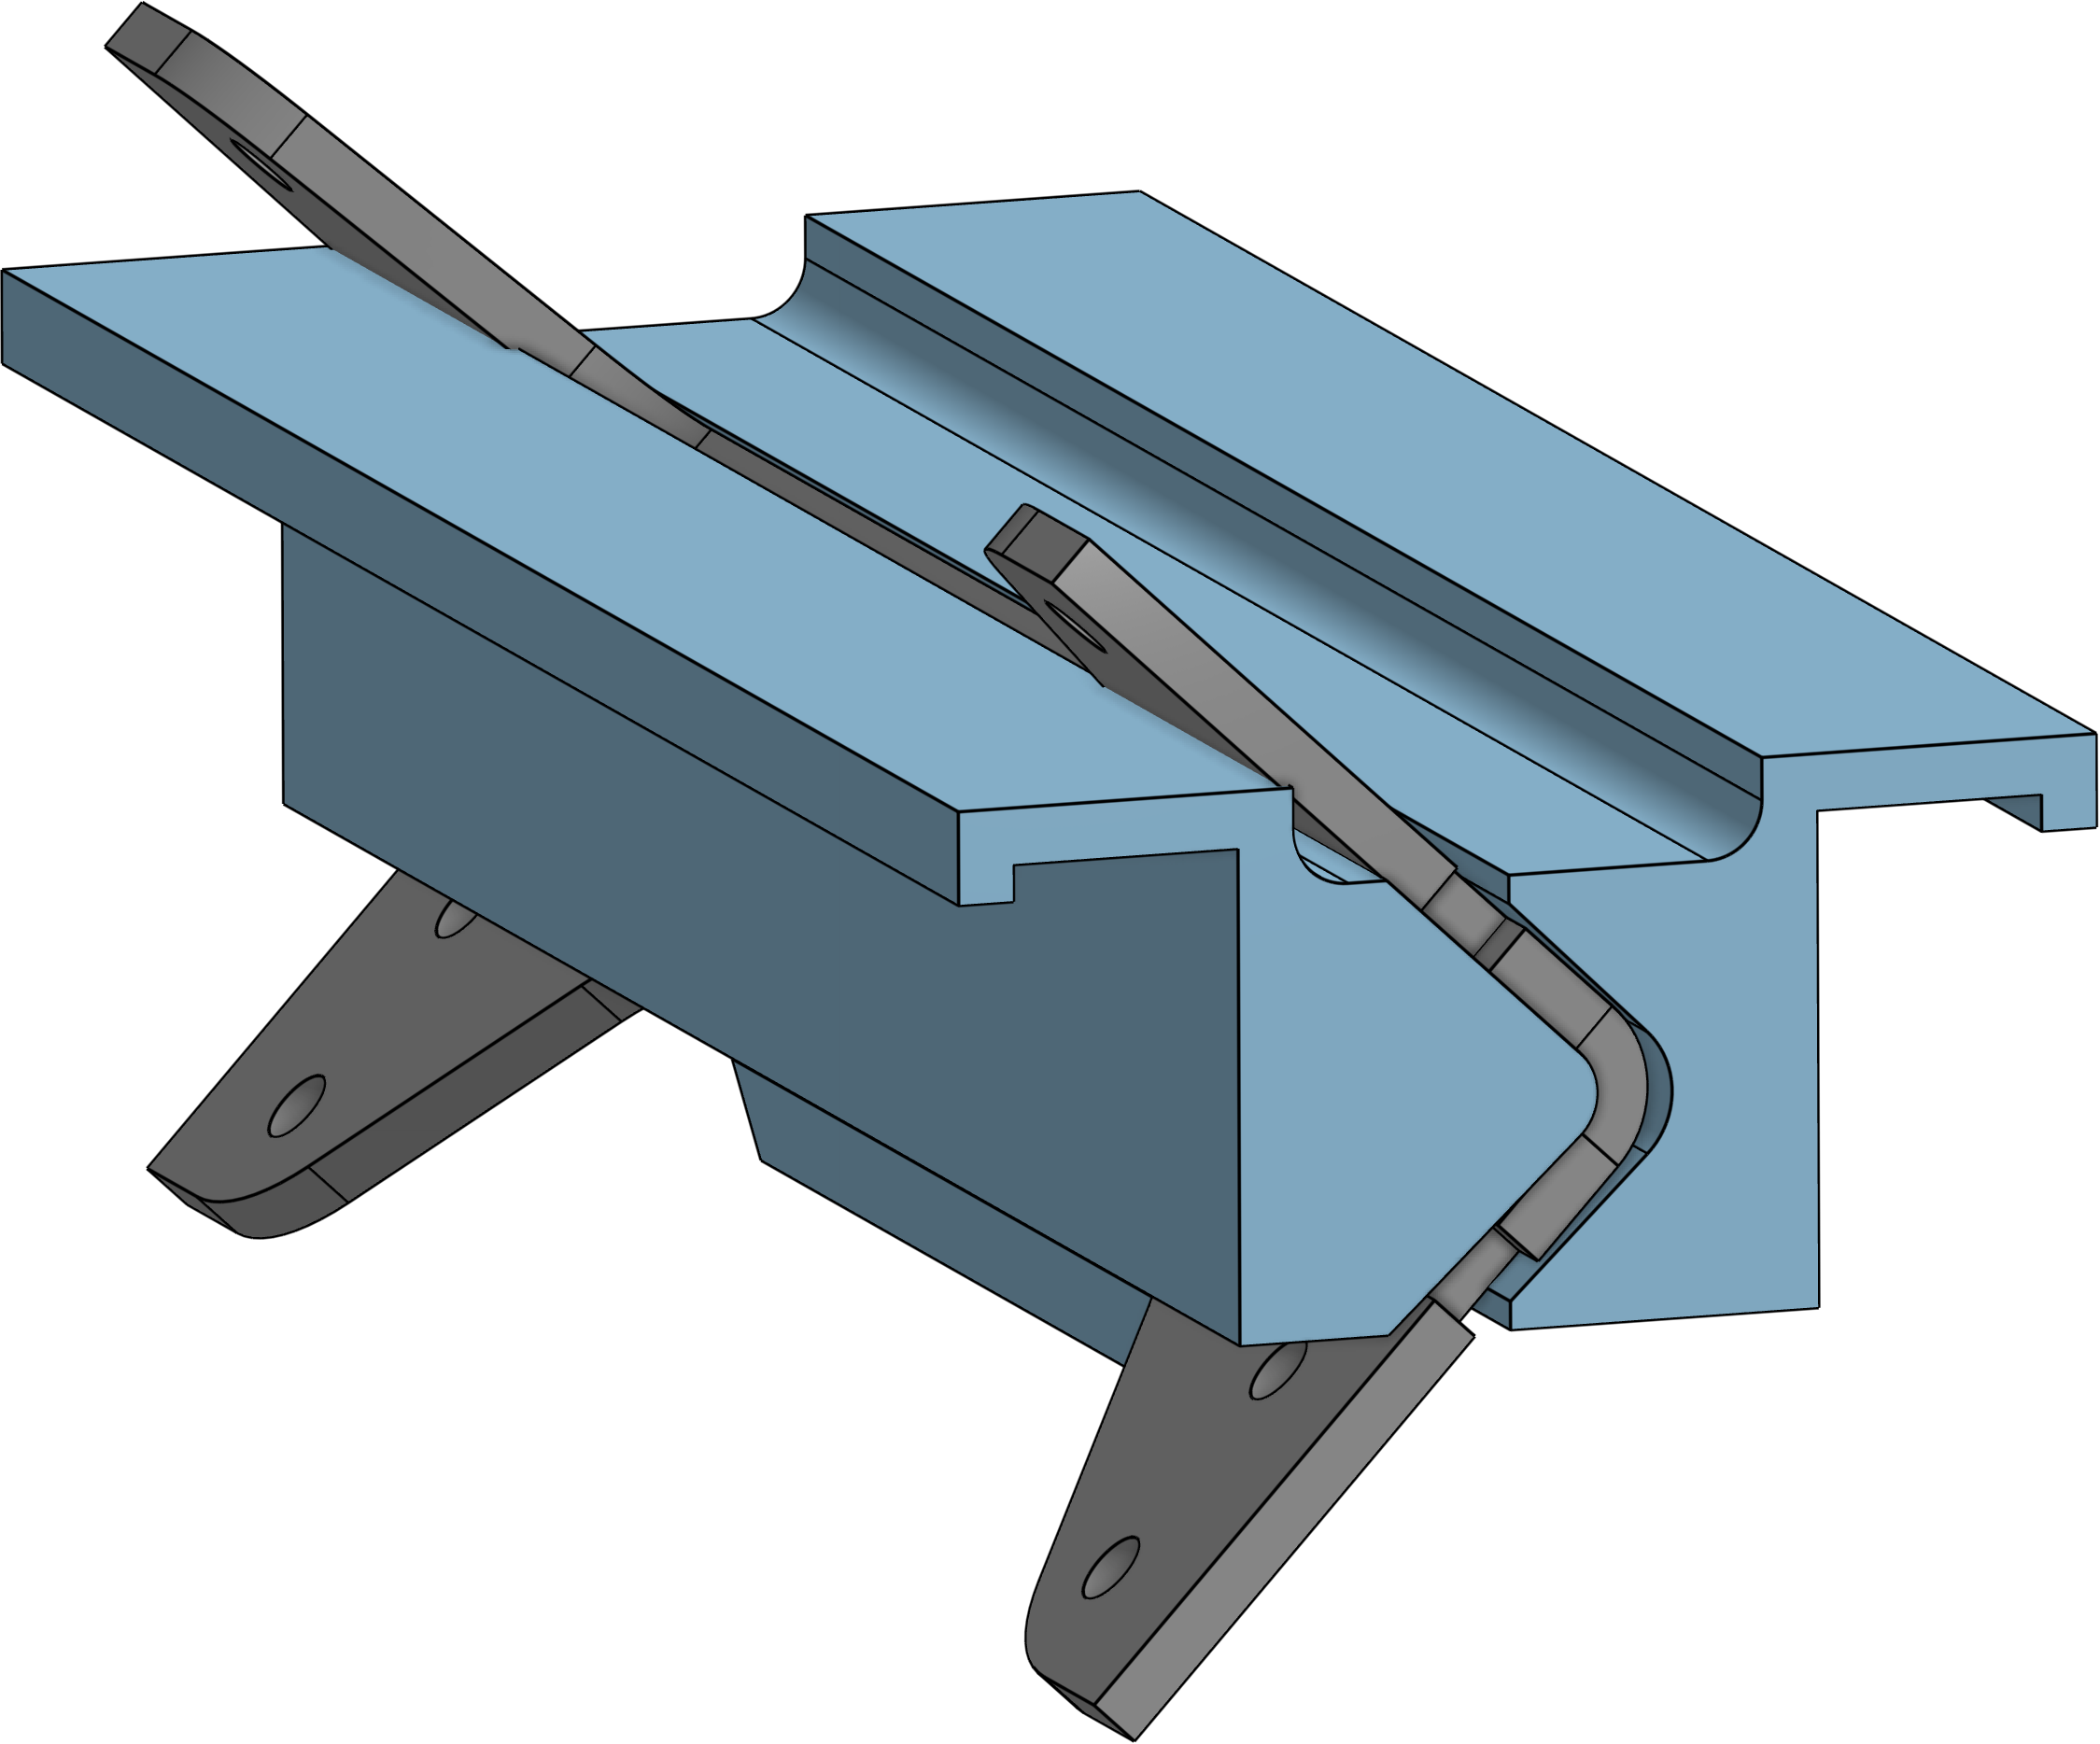
\includegraphics[width=\textwidth]{image/fabrication/corner_bent.png}
        \end{minipage}
        \caption{Fabricación del Corner con matriz y punzón impreso en 3D.}
        \label{fig:fabricacion.corner}
      \end{figure}
      \begin{figure}[!ht]
        \centering
        \begin{minipage}{.32\textwidth}
          \centering
          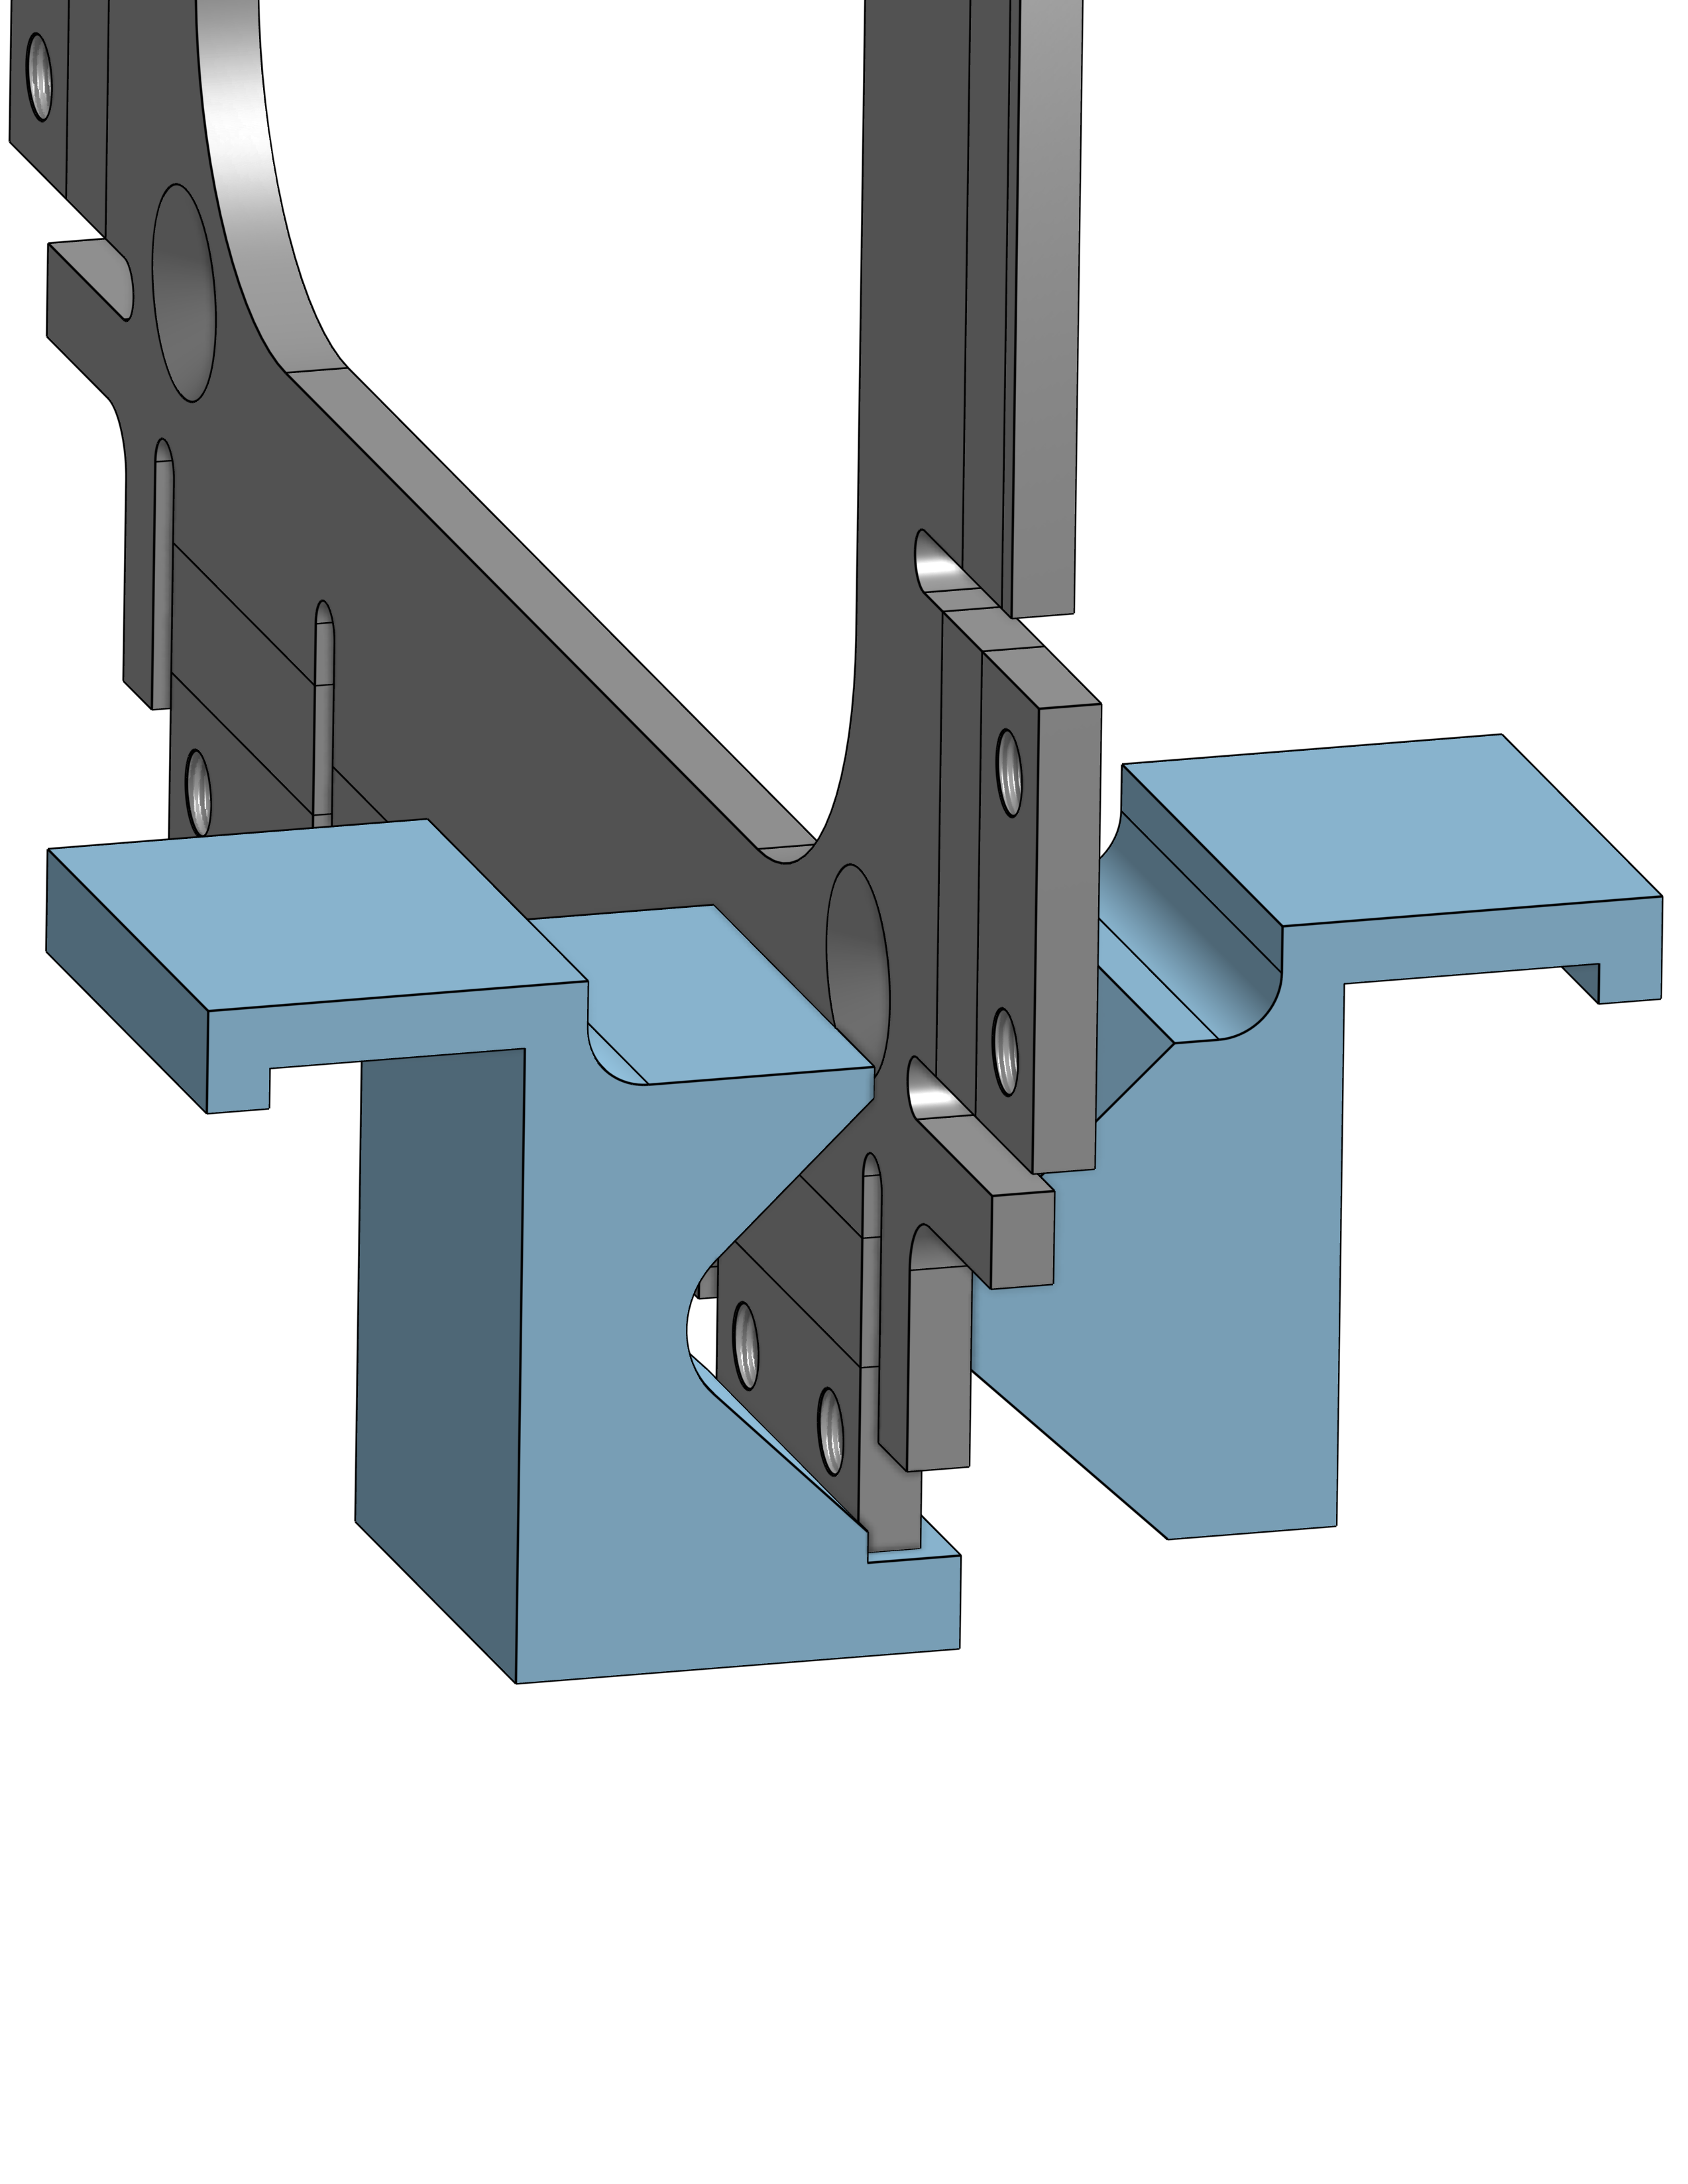
\includegraphics[width=\textwidth]{image/fabrication/lid_flat.png}
        \end{minipage}
        \hspace{3cm}
        \begin{minipage}{.32\textwidth}
          \centering
          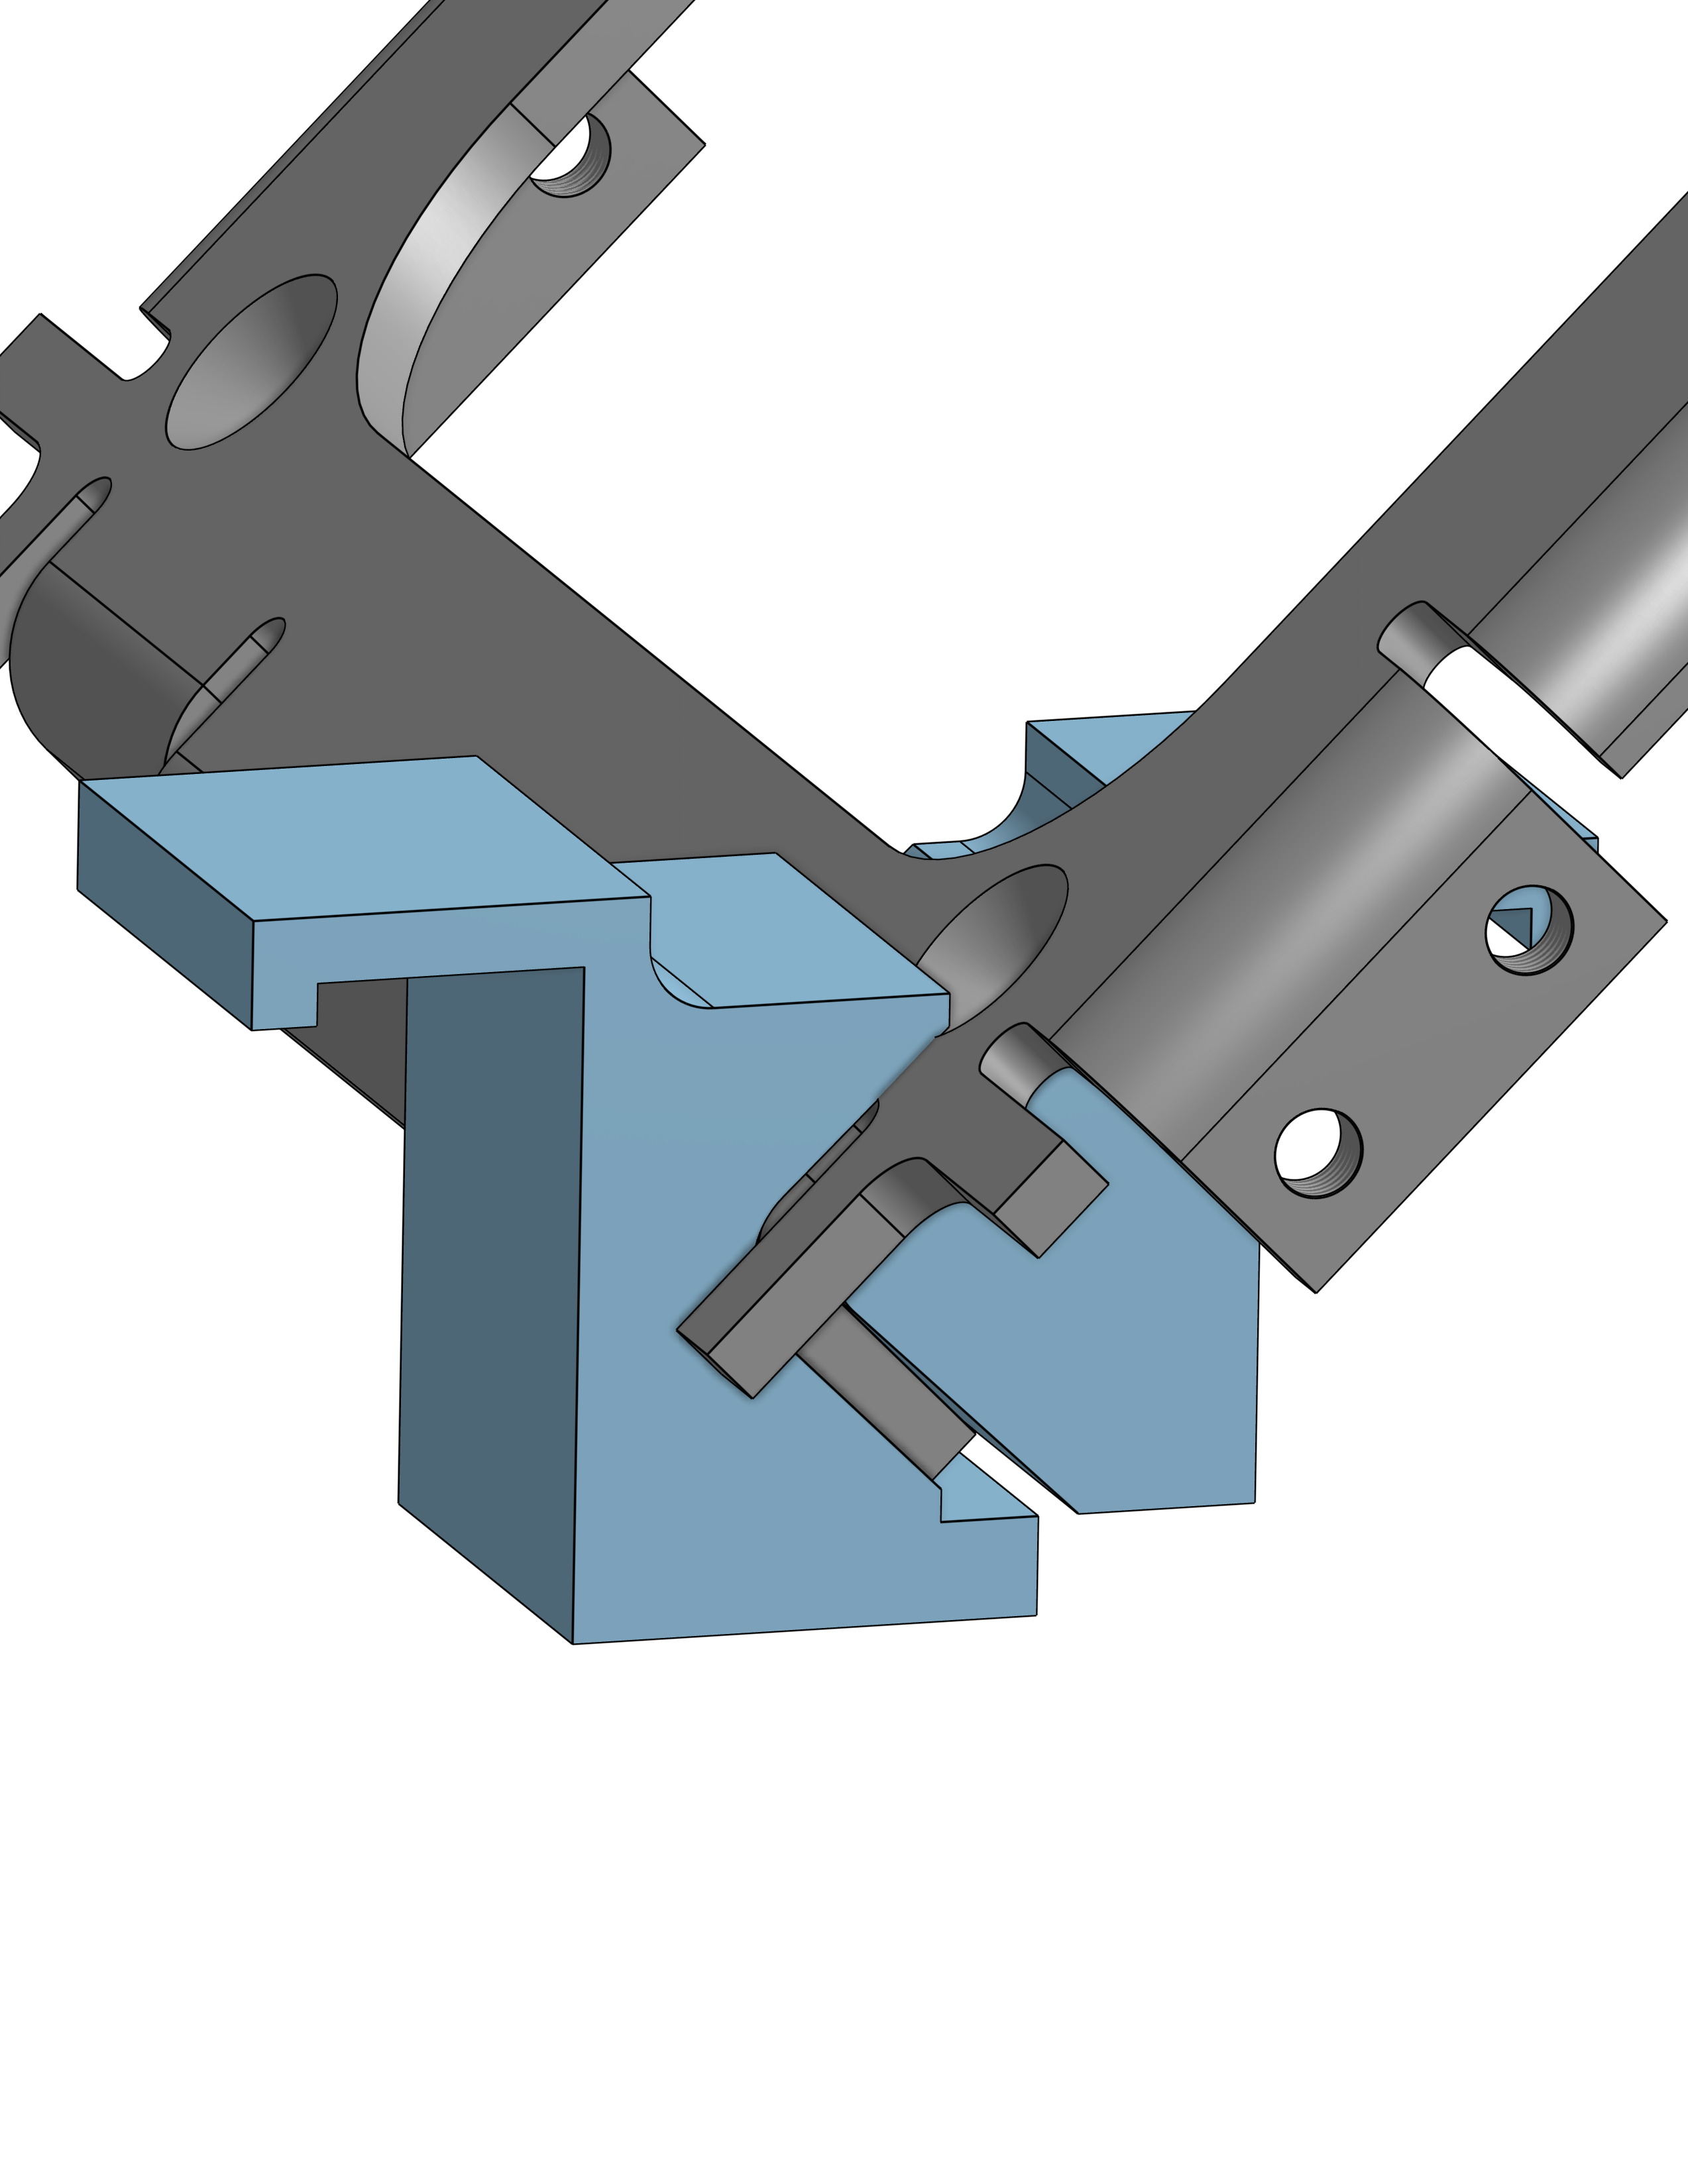
\includegraphics[width=\textwidth]{image/fabrication/lid_bent.png}
        \end{minipage}
        \caption{Fabricación del Lid con matriz y punzón impreso en 3D.}
        \label{fig:fabricacion.lid}
      \end{figure}
      \begin{figure}[H]
        \centering
        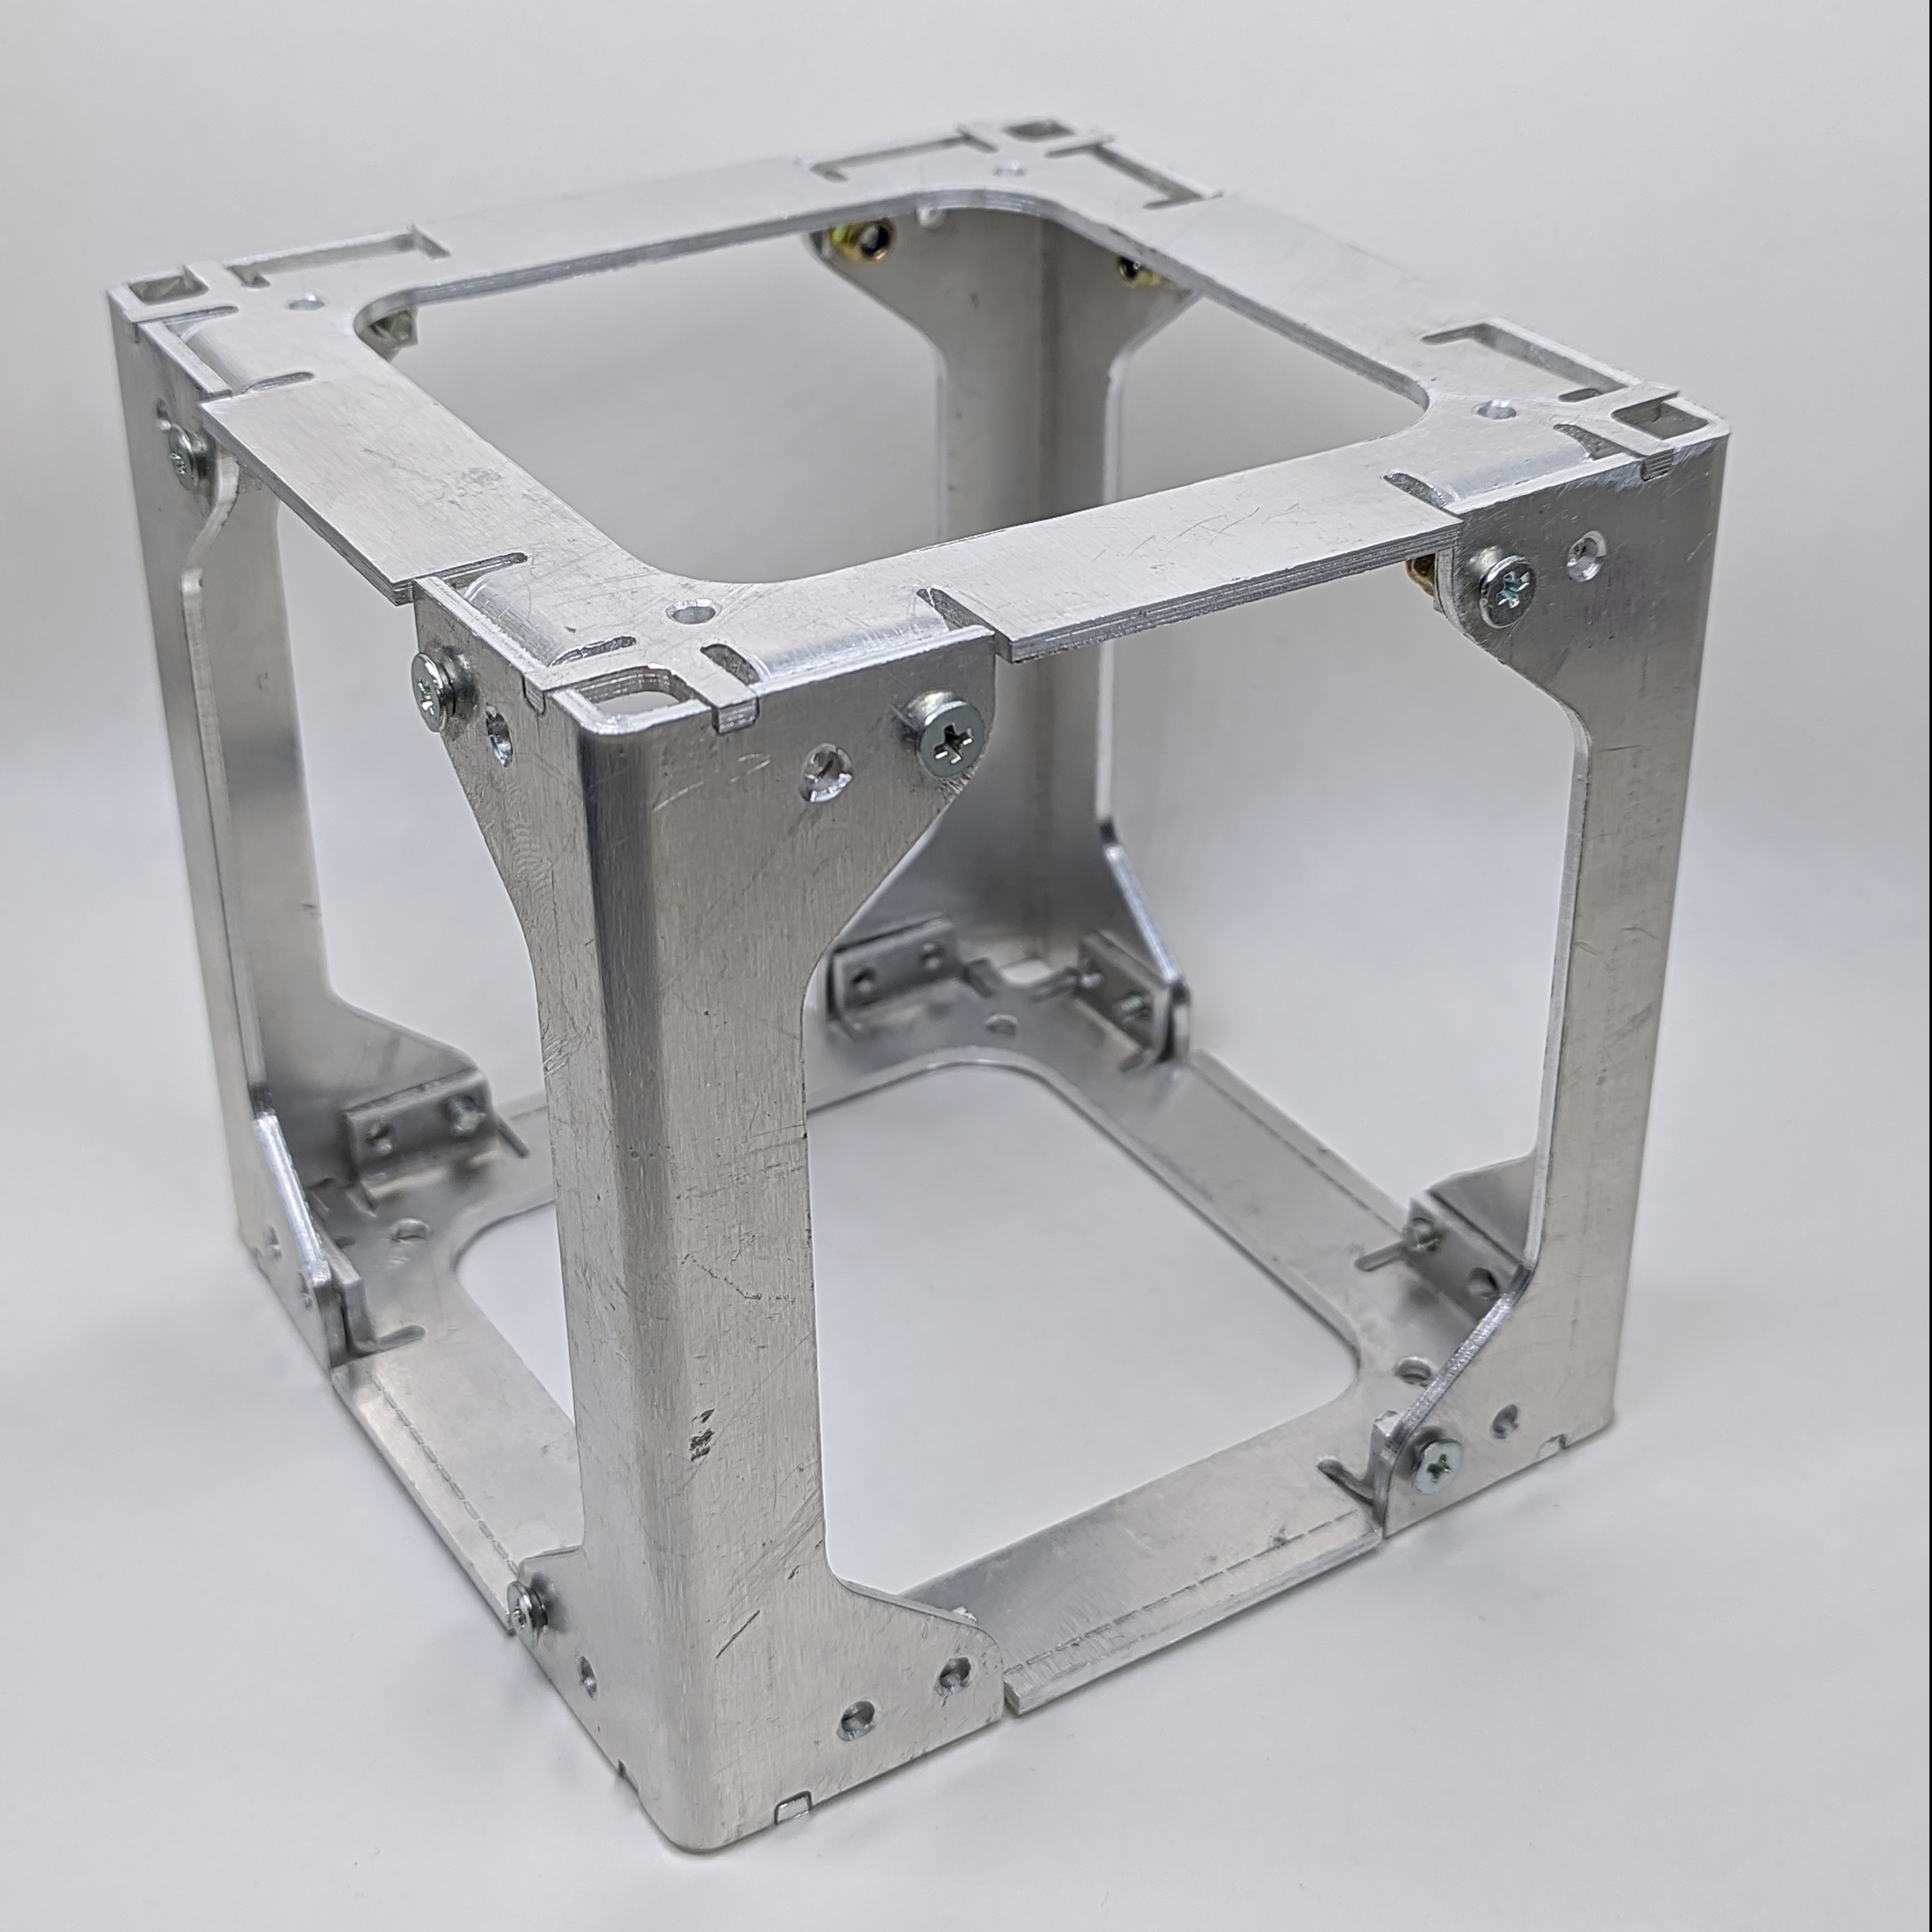
\includegraphics[width=0.6\textwidth]{image/fabrication/prototype.jpg}
        \caption{Prototipo plegado con herramientas impresas en 3D.}
        \label{fig:fabricacion.prototipo1}
      \end{figure}

    \subsubsection{Colocación de Muestras}
      La estructura del CubeSat permitirá que las muestras se puedan colocar después de finalizar el ensamblaje de la
      estructura. Esto se hace posible gracias a las aberturas de las tapas, de las cuales la del plano +Z, va a ser
      para acceder a una tapa en la carcasa que aloje el módulo de carga útil, y por donde se carguen las muestras a
      analizar. Esta tapa va a ser fijada con la tornillería correspondiente

      \begin{figure}[H]
        \centering
        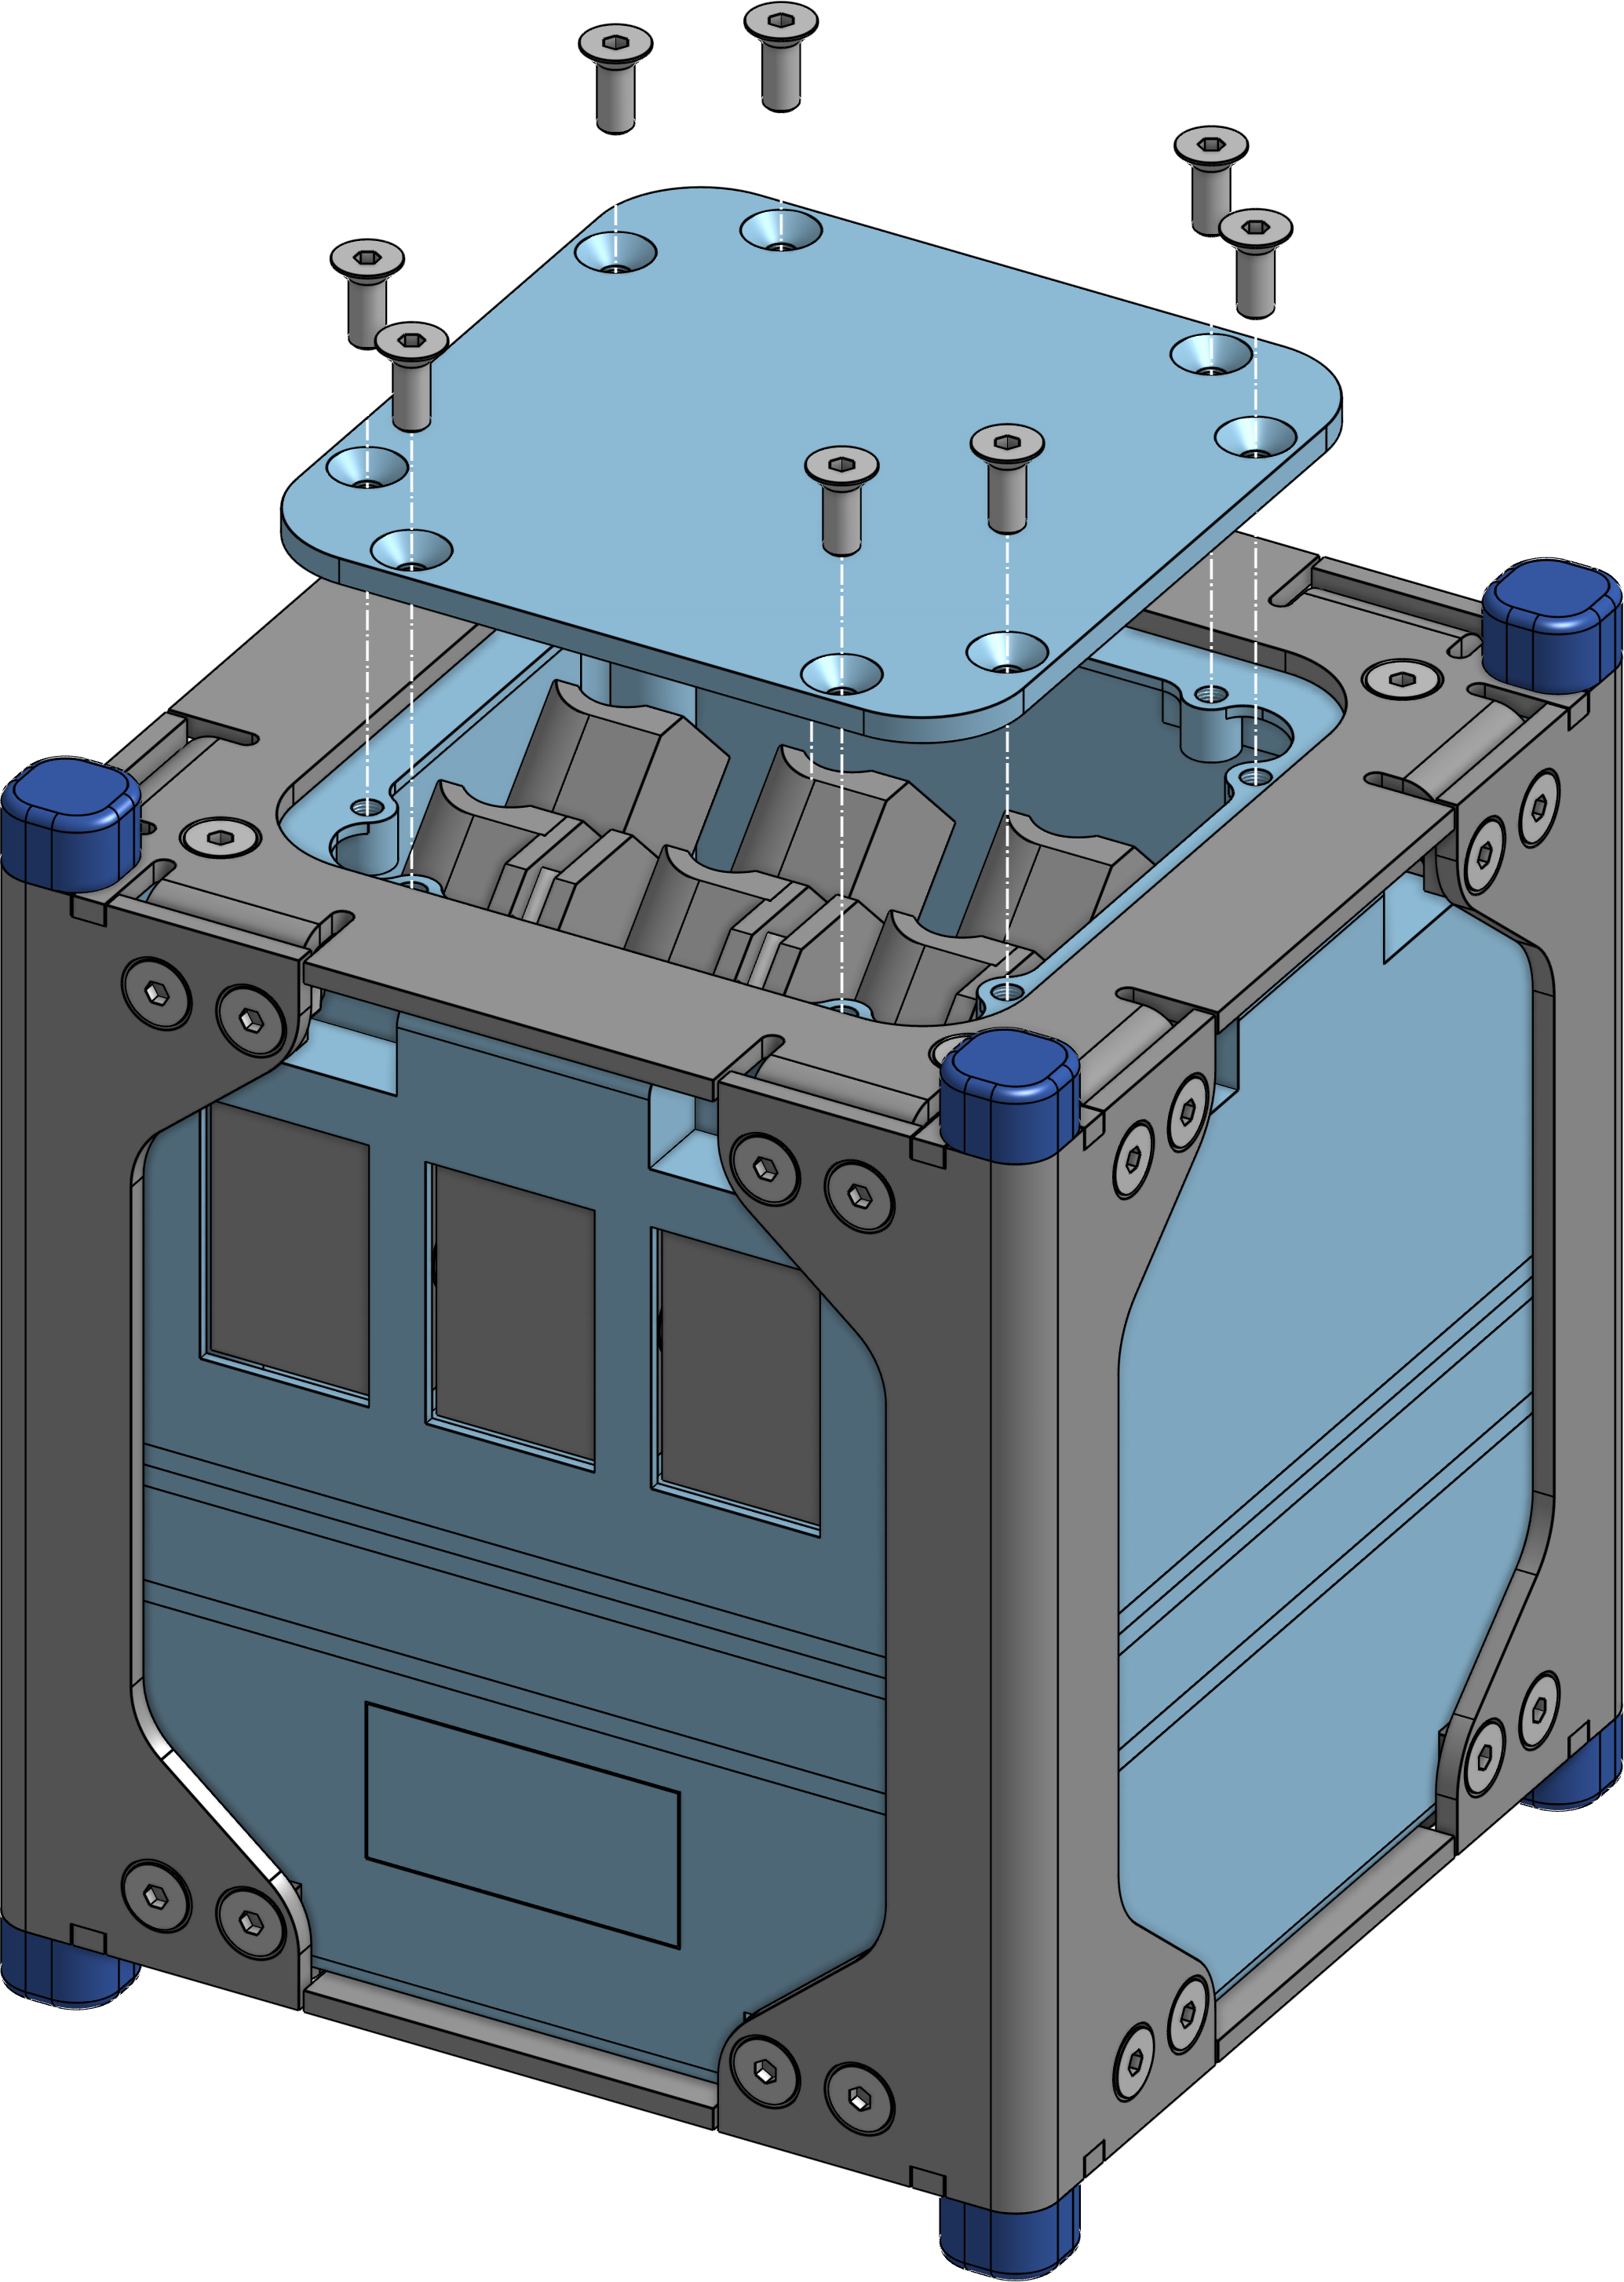
\includegraphics[width=0.4\textwidth]{image/structure/muestras.png}
        \caption{Colocación de muestras}
        \label{fig:structure-muestra}
      \end{figure}

  \subsection{Electronica}
    La electrinica del CubeSat es, en gran parte, digital. Se buscó tener una separacion rigurosa entre la electronica
    que maneja las fuentes y la potencia, con la electronica que maneja la logica y almacenaje de datos. Por ello, él
    CubeSat tendra dos placas: Una en el \acrshort{pms} y otra en el \acrshort{obc}.

    \subsubsection{Placa \acrshort{obc}}
      La placa del \acrshort{obc} alberga el cerebro del CubeSat. En ella, estara la Raspberry Pi Zero 2 W, la cual es
      la encargada de leer todos los sensores, almacenar los datos y controlar el resto de los subsistemas del CubeSat.
      En esta placa, se encontrará la \acrshort{imu} MPU9250 y el sensor de presion y temperatura BMP280. Además, por
      medio del conversor analogico a digital ADS1115, la Raspberry lee los sensores de temperatura de la \acrshort{pu},
      con los cuales comanda a la \acrshort{pms} para regular la temperatura.

      La comunicacion entre la \acrshort{obc} y la \acrshort{pms} es realizada mediante el protocolo $I^2C$. La
      Raspberry Pi cumpliria el rol de "Master", mientras que el resto de los sensores, y la \acrshort{pms} cumplirian
      el rol de "Slave".

      Cabe destacar, que al momento de diseñar la placa, se priorizara tener la menor cantidad de componentes en formato
      "PCB con Pines macho". En algunos casos (por ejemplo, el MPU9250 o la Raspberry), nuestras capacidades de fabricacion
      no son tan altas, por lo que ciertos componentes permaneceran en su formato de placa, y se montaran sobre la placa
      que fabriquemos.

      Revise la sección \ref{anexo:obc.schematic} para ver el esquemático del \acrfull{obc}. En la tabla
      \ref{tab:electronica.bom.obc} puede ver la lista de materiales para la placa del \acrshort{obc}.

      \begin{table}[!ht]
        \centering
        \begin{tabular}{|c|c|}
          \hline
          \textbf{Item}           & \textbf{Cantidad} \\ \hline
          Resistencias            & 9 \\ \hline
          Capacitores             & 3 \\ \hline
          Fusibles                & 3 \\ \hline
          Conectores              & 3 \\ \hline
          Raspberry Pi Zero 2 W   & 1 \\ \hline
          Barometro BMP280        & 1 \\ \hline
          \acrshort{imu} MPU9250  & 1 \\ \hline
          \acrshort{adc} ADS1115  & 1 \\ \hline
          Termistores NTC 100K    & 3 \\ \hline
        \end{tabular}
        \caption{Lista de Materiales para la placa \acrshort{obc}}
        \label{tab:electronica.bom.obc}
      \end{table}

    \subsubsection{Placa \acrshort{pms}}
      La placa del \acrshort{pms} alberga todo lo que es fuentes de voltaje, monitoreo y control de potencia. Él
      componente central de esta placa es el Atmega328P, un microcontrolador de propósito general el cual se encarga de
      recibir comandos via $I^2C$ de la \acrshort{obc} y reportar las diferentes lecturas o ejecutar órdenes. Además, él
      \acrshort{pms} da la posibilidad al CubeSat de ser alimentado externamente, sin consumir las baterías.

      Para las fuentes, la \acrshort{pms} implementa tres fuentes DC-DC del tipo "Buck". Estas fuentes (modelo HW-133B)
      vienen en formato de "PCB" o "Módulo Arduino". Como el integrado y los componentes son manejables, y los
      requerimientos para hacer una placa con esos componentes no son tan elevados, se decidió hacer que las fuentes sé
      integren en el diseño del circuito impreso, y que los componentes se monten directamente sobre ella, sin ninguno
      otra PCB entre medio. Además, esto es necesario, ya que el integrado DC-DC MP1584EN que usan las fuentes, tienen
      un pin de control de salida, por lo que podemos con el Atmega328P, elegir el estado de la salida. En él
      formato "PCB" de la fuente, el pin de activación no está disponible. Este detalle es importante, ya que permite
      poder reducir el consumo cuando no es necesario tener todos los subsistemas activos. Como un extra, se agregó un
      sensor de corriente INA219 para tener una medición del consumo de corriente durante la misión. Este sensor, nos
      permite, en conjunto con las mediciones de voltaje, tener un muy buen estimativo de la energía consumida, y por
      lo tanto tener un estimativo de la energía disponible o restante.

      La \acrshort{pms} implementa un sistema de "Arbitraje de fuente" utilizando MOSFETs y Amplificadores
      Operacionales. Esto significa que el CubeSat, tiene más de una fuente de energía disponible y puede priorizar la
      Utilización de una sobre otra. En este caso, el CubeSat tiene 2 posibles fuentes: La batería interna o una fuente
      externa. La fuente externa tiene prioridad respecto de la batería. Cuando esta se conecta, la batería queda
      electrónicamente desconectada del PMS y todo el CubeSat se alimenta de la fuente externa. Debido a la complejidad
      de carga de la batería, se optó por no permitir que la batería se cargue cuando se conecte la fuente externa. Él
      cambio entre batería y fuente externa no provoca ningún fenómeno o interrupción en la operación del CubeSat.

      Para el control de la \acrshort{tru}, el \acrshort{pms} implementa dos integrados de puente H L298N para poder
      controlar la polaridad y la potencia de las celdas Peltier. El puente H tiene varios modos de polaridad
      disponibles. Para nuestra aplicación, solo se utilizan los modos "Clockwise" y "CounterClockwise", que básicamente
      invierten la polaridad. Para el control de la potencia, el Atmega328P genera tres señales cuadradas con capacidad
      de ser moduladas por ancho de pulso (PWM).

      Para ahorrar energía, el \acrshort{pms} tiene conectado el \acrshort{hmi}. Dependiendo del estado, diferentes
      raíles y subsistemas son activados o desactivados. Cuando se coloca la llave de "Apagado", el \acrshort{pms} envía
      al \acrshort{obc} un aviso de que debe apagarse. Esto garantiza que todos los archivos fueron escritos y todos los
      programas terminados, para tener un apagado seguro de la Raspberry. Una vez completado el apagado, el Atmega328P
      apaga todas las fuentes y se pone en reposo hasta que cambie el estado del \acrshort{hmi}. Esto es posible gracias
      a que la fuente DC-DC permanece encendida en todo momento, y es un MOSFET el que se desactiva, apagando el raíl de
      5V para el resto del CubeSat.

      Por una falta de pines en el Atmega328P, se utiliza el conversor analogico a digital ADS1115 y el expansor de
      $I^2C$ a paralelo PCF8574. Estos, estaran conectados a un bus $I^2C$ secundario, en el cual el Atmega328P actuara
      como "Master" y el resto de los sensores como "Slave".

      A travez del $I^2C$, la \acrshort{obc} solicita datos al Atmega328P. Estos datos pueden ser: Voltajes de todas las
      fuentes, voltaje de la batería, voltaje de las celdas, temperatura de la batería, consumo de corriente total
      actual y estado del HMI. Además, puede escribir estados y variables, como: Estado de las fuentes, estado de la 
      alimentación y potencia de las celdas Peltier por individual.

      Revise la sección \ref{anexo:pms.schematic} para ver el esquemático del \acrfull{pms}. En la tabla
      \ref{tab:electronica.bom.obc} puede ver la lista de materiales para la placa del \acrshort{pms}.

      \begin{table}[H]
        \centering
        \begin{tabular}{|c|c|}
          \hline
          \textbf{Item}               & \textbf{Cantidad} \\ \hline
          Resistencias                & 39 \\ \hline
          Capacitores                 & 31 \\ \hline
          Diodos                      & 4 \\ \hline
          Polyfuses                   & 7 \\ \hline
          Conectores                  & 8 \\ \hline
          MOSFETs                     & 2 \\ \hline
          ATmega328P-A                & 1 \\ \hline
          Sensor de Corriente INA219  & 1 \\ \hline
          Fuente DC-DC HW-133B        & 3 \\ \hline
          \acrshort{adc} ADS1115      & 1 \\ \hline
          Inversor 4069               & 1 \\ \hline
          Puente H L298HN             & 2 \\ \hline
          OpAmp LM2904                & 1 \\ \hline
          Expansor I2C PCF8574AT      & 1 \\ \hline
          Cristal (16 MHz)            & 1 \\ \hline
          Termistor NTC 100K          & 1 \\ \hline
          Celdas 18650                & 5 \\ \hline
        \end{tabular}
        \caption{Lista de Materiales para la placa \acrshort{pms}}
        \label{tab:electronica.bom.pms}
      \end{table}

  \subsection{Criterios de Márgenes}
    Para en análisis de presupuestos preliminares establecimos los márgenes considerando las condiciones más
    desfavorables

    \subsubsection{Presupuesto Preliminar de Masa}
      El presupuesto de masa se calcula considerando que la estructura y las baterías tienen prioridad para ser
      integradas.
      \begin{table}[H]
        \centering
        \begin{tabular}{|c|c|c|c|}
          \hline
          \textbf{Elemento} & \textbf{Cantidad} & \textbf{Peso simple}  & \textbf{Subtotal} \\ \hline
          Lids              & 2                 & $26.8 \, g$           & $53.6 \, g$ \\ \hline
          Corners           & 4                 & $17.8 \, g$           & $71.2 \, g$ \\ \hline
          Varillas          & 4                 & $13.8 \, g$           & $55.2 \, g$ \\ \hline
          Tornillos M3      & 78                & $0.5 \, g$            & $39 \, g$ \\ \hline
          Tuercas M3        & 32                & $0.5 \, g$            & $16 \, g$ \\ \hline
          Baterías 18650    & 5                 & $46 \, g$             & $230 \, g$ \\ \hline
          Raspberry Pi Zero & 1                 & $12.1 \,g$            & $12.1 \, g$ \\ \hline
          Carcasas Subsust. & -                 & $0,92 \, g/cm^3$      & $170 \, g$ \\ \hline
          Unidad Termoregul.& 3                 & $64 \, g$             & $192 \, g$ \\ \hline
          \textbf{Total}    & -                 & -                     & $839.1 \, g$ \\ \hline
        \end{tabular}
        \caption{Presupuesto de Pesos.}
      \end{table}

      Consideramos que con el margen de aproximadamente $160 \, g$ sobrantes, los componentes de cada subsistema
      (placas, integrados, módulos, cables, soldaduras, etc.) el CubeSat se mantendrá dentro del régimen de $1 \, Kg \pm
      20 \, g$ adaptando su posterior diseño a estas condiciones. Se considera un margen del 10\% de error, lo que
      dejaría al CubeSat en aproximadamente $80 \, g$ sin placas. En caso de ser necesario, se agregarán pesos
      muertos para llegar al régimen o se realizarán recortes en las caras de las carcasas. Algo a tener en cuenta es
      que el peso final de las carcasas va a ser menor debido a que el cálculo realizado no tiene en cuenta la
      posibilidad de hacer rellenos vacíos como lo hacen las impresoras 3D FDM.

    \subsubsection{Presupuesto Preliminar de Potencia}
      El presupuesto de potencia se calculó considerando el caso más desfavorable que se puede dar en cada uno de los
      componentes.

      \begin{table}[H]
      \centering
      \resizebox{\textwidth}{!}{
      \begin{tabular}{|l|c|c|c|c|c|c|}
      \hline
      \textbf{Componente} & \textbf{Cant.} & \textbf{Tensión [V]} & \textbf{Corriente [mA]} & \textbf{Potencia [W]} & \textbf{Subtotal [W]} & \textbf{@ 18V[A]} \\
      \hline
      Raspberry Pi Zero 2 W & 1 & 5.0  & 260 & 1.3       & 1.3    & 72.2 m \\
      Atmega328p            & 1 & 5.0  & 5.2 & 26 m      & 26 m   & 1.4 m  \\
      Sensor BMP280         & 1 & 3.3  & 0.7 & 2.3 m     & 2.3 m  & 0.13 m \\
      Sensor MPU9250        & 1 & 3.3  & 3.9 & 13 m      & 13 m   & 0.72 m \\
      Puente H L298n        & 2 & 2    & $\approx 1$   & $\approx 2$ & 2 & 110 m  \\
      Módulo ADS1115 (ADC)  & 2 & 3.3  & 0.2 & 0.66 m    & 1.32 m & 0.073 m \\
      Celdas Peltier 3x3 cm & 3 & 12.0 & 833 & 10.00     & 30.00  & 1.66   \\
      \hline
      \textbf{Total}        & – & –   & –      & –      & \textbf{33.35} & \textbf{1.9} \\
      \hline
      \end{tabular}
      }
      \caption{Consumo de corriente y potencia de los componentes en el caso más desfavorable.}
      \label{tab:consumo_componentes}
      \end{table}

      Para la misión elegimos tener 5 celdas 18650 de 3.6 V cada una con una capacidad de 3350 mAh y una capacidad
      máxima de descarga de 1.5A \cite{datasheet-cmicr18650-f9l}. Se dispondrán todas en serie, teniendo un voltaje
      nominal de 18V a 3350mAh. Esto nos dará un tiempo de autonomía de 105 minutos. Esto es considerando el caso más
      desfavorable, el cual sería que las zonas térmicas irradian toda su energía térmica al ambiente, haciendo que las
      Peltier estén siempre al máximo de consumo permitido (10W). Para el futuro, se buscará hacer ensayos reales del
      consumo de cada componente y se buscará que cada uno de ellos sea el menor posible, pero como estimativo, y
      considerando una temperatura ambiente de $25\Celsius$, las celdas Peltier consumirán al rededor de 2 a 5W para un
      $\Delta T = 20\Celsius$ \cite{datasheet-peltier}, lo cual implicaría un consumo de 20W por hora, dándonos un total
      de 3 horas de autonomía. Para determinar la potencia de los sensores se ha considerado sus respectivos datasheet
      \cite{datasheet-mpu9250} \cite{datasheet-bpm280}.
      
    \subsubsection{Presupuesto Preliminar de Datos}
      Durante el vuelo se generaban y almacenarán diversos tipos de datos relacionados tanto con la misión primaria como
      con la misión secundaria. A continuación se detalla el presupuesto preliminar de almacenamiento de datos
      considerando un periodo de recolección de 4 horas.  Cada muestra registrada incluye el instante temporal y él
      valor medido del parámetro, ocupando 4 bytes cada uno, lo que da un total de 8 bytes por muestra, a excepción que 
      se indique lo contrario. Además, consideramos la mayor frecuencia de muestreo permitida por cada sensor.

      \begin{table}[H]
      \centering
      \begin{tabular}{|l|c|}
      \hline
      \textbf{Vector} & \textbf{Tamaño de muestra} \\
      \hline
      Tiempo & 4 bytes \\
      Valor  & 4 bytes \\
      \hline
      \textbf{Tamaño total} & \textbf{8 bytes} \\
      \hline
      \end{tabular}
      \caption{Tamaño total fijo por muestra de cada parámetro}
      \label{tab:tamanio_muestra}
      \end{table}

      \begin{itemize}

        \item \textbf{Variables físicas y ambientales}

        \begin{table}[H]
          \centering
          \begin{tabular}{|c|c|c|c|}
            \hline
            \textbf{Parámetro} & \textbf{Frecuencia [Hz]} & \textbf{Muestras/4h} & \textbf{Tamaño [MB]} \\
            \hline
            Presión               & 157   & 2,260,800  & $\approx$ 17.26     \\
            Temperatura ambiente  & 157   & 2,260,800  & $\approx$ 17.26     \\
            Aceleración           & 4000  & 57,600,000  & $\approx$ 878.92   \\
            Ángulo de giro        & 8000  & 115,200,000 & $\approx$ 1757.84   \\
            \hline
            \textbf{Total estimado} & -    & -         & $\boldsymbol{\approx 2671.28}$ \\
            \hline
          \end{tabular}
          \caption{Volumen de datos total y de cada variable físico-ambiental.}
          \label{tab:volumen_datos}
        \end{table}
        Notar que en aceleración y ángulo de giro se a considerado un tamaño de muestra de 16 bytes debido a los tres ejes mas la marca de tiempo.
        
        \item \textbf{Control de temperatura de de las muestras celulares}

        \begin{table}[H]
          \centering
          \begin{tabular}{|c|c|c|c|}
            \hline
            \textbf{Parámetro} & \textbf{Frecuencia [Hz]} & \textbf{Muestras/4h} & \textbf{Tamaño [MB]} \\
            \hline
            Temperatura & 157   & 2,260,800  & $\approx$ 51.78     \\ \hline
          \end{tabular}
          \caption{Volumen de datos de los controles de temperatura de las muestras celulares}
          \label{tab:volumen_datos_temperatura}
        \end{table}
        La medida de la temperatura es 24 bytes debido a las marcas de tiempo y las temperaturas que se toman para cada una de las muestras.

        \item \textbf{Información gravada previamente}

        \begin{table}[H]
        \centering
        \begin{tabular}{|l|c|c|}
        \hline
        \textbf{Software} & \textbf{Versión} & \textbf{Tamaño} \\
        \hline
        S.O. Raspberry Pi OS Lite (Debian 12.0 "bookworm") & - & $\approx$ 2.1~GB \\
        Python                   & 3 & $\approx$ 27.5~\textit{MB} \\
        Dependencias python      & 1 & $\approx$ 150~\textit{MB} \\
        logrotate                & 1 & $\approx$ 100~\textit{KB} \\
        chrony                   & 1 & $\approx$ 2~\textit{MB} \\
        \hline
        \textbf{Total estimado}  & - & $\boldsymbol{\approx 2.3~GB}$ \\
        \hline
        \end{tabular}
        \caption{Consumo de almacenamiento de los componentes}
        \label{tab:almacenamiento_componentes}
        \end{table}
    
      \end{itemize}

      \begin{table}[H]
      \centering
      \begin{tabular}{|l|c|}
      \hline
      \textbf{Apartado} & \textbf{Tamaño estimado [MB]} \\
      \hline
      Variables físicas              & 2671.28 \\
      Back up Variables físicas      & 2671.28 \\
      Temperaturas celulares         & 51.78  \\
      Back up Temperaturas celulares & 51.78  \\
      Información grabada previamente & 2355 \\
      \hline
      \textbf{Tamaño total}          & \textbf{7801.12} \\
      \hline
      \end{tabular}
      \caption{Tamaño total estimado}
      \label{tab:tamano_total_estimado}
      \end{table}

      Teniendo en cuenta todos los datos a ser almacenados, estimamos un volumen total de
      aproximadamente 7.62 GB.

\section{Secuencia de Operación}
  Para llevar a cabo la misión, se prevé seguir con la siguiente secuencia:

  \begin{itemize}
    \item \textbf{Etapa 1:} Cultivo de muestras.
        48hs previo al día de lanzamiento se procede con el cultivo de las muestras biológicas siguiendo el procedimiento descrito en la sección  \ref{sec:procedimientos-prev-lanzamiento}.
   \item \textbf{Etapa 2:} Traslado de muestras.
      Se buscan las muestras previamente cultivadas y se sigue con el procedimiento de traslado descrito en la sección \ref{sec:procedimientos-prev-lanzamiento}.
    \item \textbf{Etapa 3:} Arranque del CubeSat.\\
      Una vez en el lugar de lanzamiento, se coloca la llave correspondiente en el \acrshort{hmi} físico para establecer el modo de Pre Lanzamiento, en el cual
      se inicializan todos los subsistemas. En esta etapa, el CubeSat será conectado a una fuente de alimentación externa para alcanzar él
      régimen permanente de las distintas temperaturas controladas sin consumir energía extra de las baterías.
    \item \textbf{Etapa 4:} Validación de los sistemas.\\
      Mientras el CubeSat estabiliza la temperatura en modo Pre Lanzamiento, se abre un canal de comunicación con él
      CubeSat vía WiFi. Así, se podrá monitorear el estado de los sensores, los voltajes y consumos reportados de las
      baterías, para verificar que se encuentren en niveles óptimos y totalmente operativos.
    \item \textbf{Etapa 5:} Colocación de las Muestras.\\
      Una vez que la temperatura de la bahía de muestras esté estabilizada, se destapa la
      bahía de muestras para la colocación de las mismas. Luego, se vuelve a colocar la tapa y se espera a que las temperaturas
      correspondientes se estabilizan.
    \item \textbf{Etapa 6:} Preparación para el lanzamiento.\\
      Con el CubeSat en estado de Pre Lanzamiento, todos los sensores verificados, y todas las muestras cargadas, sé
      procede desconectar la fuente de alimentación externa, y cargar el CubeSat a la bahía de
      carga del Cohete. En este estado, el CubeSat seguirá teniendo el puerto de comunicación vía WiFi disponible, hasta
      que se retire la llave de Pre Lanzamiento o "Remove Before Flight".
    \item \textbf{Etapa 7:} Lanzamiento, apogeo y aterrizaje.\\
      Luego de retirar la llave de Pre Lanzamiento, el CubeSat está preparado para la misión. Durante esta etapa
      no hay telemetría, ni parámetros para monitorear en tiempo real.
    \item \textbf{Etapa 8:} Recuperación del CubeSat.\\
      Una vez recuperado el CubeSat, se coloca la llave de recuperación de datos y se conecta la fuente de
      alimentación externa al CubeSat para evitar agotar la energía de las baterías y mantener las muestras estables. Luego, sé
      extrae las muestras de la bahía de muestras y se las coloca en el dispositivo de traslado nuevamente.
      Al mismo tiempo, se procede a la descarga de los datos del CubeSat en una plataforma local para su posterior procesamiento.
      Una vez finalizada la recuperación de datos, se puede colocar la llave de apagado del CubeSat y desconectar la fuente externa.
    \item \textbf{Etapa 9:} Traslado de muestras.\\
        Se trasladan las muestras al laboratorio donde serán analizadas, siguiendo mismo procedimiento descrito en la sección \ref{sec:procedimientos-prev-lanzamiento}
    \item \textbf{Etapa 10:} Control de las muestras.\\
      Se procede al análisis de las muestras siguiendo el procedimiento descrito en la sección \ref{sec:procedimientos-ensayo}.
    \item \textbf{Etapa 11:} Procesamiento de datos.\\
      Con los datos del CubeSat descargados y guardados en un lugar seguro, se realiza el procesamiento de los mismos utilizando las
      herramientas de software desarrolladas, con el fin buscar patrones y equipararlos con los resultados de los ensayos
      de las muestras biológicas.
  \item \textbf{Etapa 11:} Presentación de los datos.\\
      Se elabora un informe con conclusiones respecto a los resultados obtenidos durante el lanzamiento.
  \end{itemize}

\section{Aseguramiento de Misión}

  \subsection{Análisis de Confiabilidad}
    Para el análisis de la confiabilidad de la estructura del CubeSat, se empleó el suite de herramientas de ANSYS, en
    su versión educativa. El suite provee un extenso catálogo de herramientas de análisis y simulaciones y a su vez un
    amplio catálogo de materiales con todas sus propiedades. Para nuestro CubeSat, decidimos emplear los análisis
    modales, de vibraciones aleatorias y de estructura estática, de los cuales obtuvimos métricas como la fatiga en
    diferentes puntos de la estructura, deformaciones dadas, las condiciones de prueba y factor de seguridad para
    diferentes puntos.

    Para las simulaciones fue necesario elegir un material para cada elemento separado que forma parte de la estructura.
    En el Cuadro \ref{tab:materiales_empleados} se puede ver la lista de materiales empleados y algunas de sus
    propiedades importantes.

    \begin{table}[H]
    \centering
    \resizebox{\textwidth}{!}{
    \begin{tabular}{|p{2.2cm}|p{2.3cm}|p{2.3cm}|p{2.5cm}|p{2cm}|p{2.5cm}|}
    \hline
    \textbf{Material} & \centering\textbf{Módulo de elasticidad} & \centering\textbf{Límite Elástico} & \centering\textbf{Límite de Rotura} & \centering\textbf{Densidad} & \centering\textbf{Usado en} \tabularnewline
    \hline
    Aleación de Aluminio & \centering $71 \cdot 10^9\,Pa$ & \centering $280 \cdot 10^6\,Pa$ & \centering $310 \cdot 10^6\,Pa$ & \centering $2770\,kg/m^3$ & Tapas y Esquinas \tabularnewline
    \hline
    Acero 4140 & \centering $212.5 \cdot 10^9\,Pa$ & \centering $652.2 \cdot 10^6\,Pa$ & \centering $1015 \cdot 10^6\,Pa$ & \centering $7850\,kg/m^3$ & Tornillería y Varillas \tabularnewline
    \hline
    Polipropileno & \centering $1461 \cdot 10^6\,Pa$ & \centering $34.6 \cdot 10^6\,Pa$ & \centering $37.62 \cdot 10^6\,Pa$ & \centering $903.4\,kg/m^3$ & Rieles de Apoyo y carcasas \tabularnewline
    \hline
    \end{tabular}
    }
    \caption{Lista de materiales empleados.}
    \label{tab:materiales_empleados}
    \end{table}
    \newpage

    \subsubsection{Preparación del modelo}
      \begin{wrapfigure}{r}{0.4\textwidth}
        \vspace{-0.5cm}
        \centering
        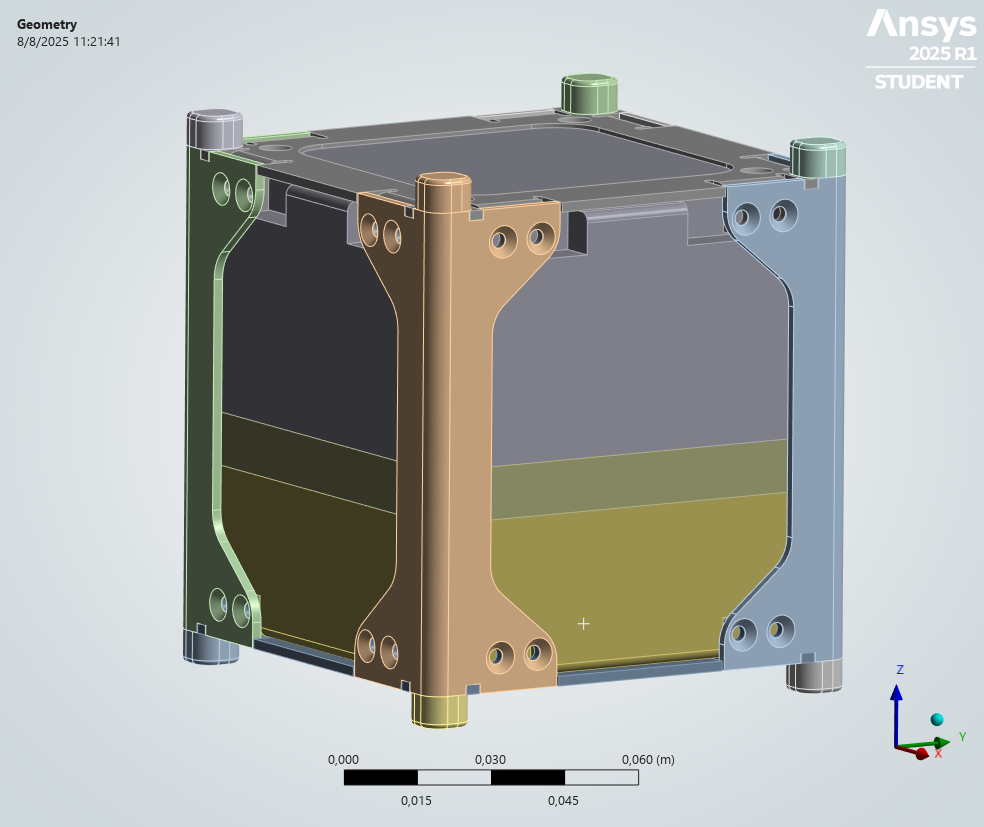
\includegraphics[width=0.4\textwidth]{image/fem/ansys_cubesat-geometry.png}
        \caption{Geometría importada}
        \label{fig:fem_geo}
      \end{wrapfigure}
      \hspace*{2em}
      El ensamblaje del CubeSat se exporta desde la plataforma de CAD online utilizada (Onshape) en formato STEP. De
      ahí, se importa la geometría a ANSYS Mechanical, el cual nos permite crear la selección y asignación de los
      materiales, fijar superficies de contacto y establecer superficies de fijación. Luego de importar la geometría,
      ANSYS Mechanical automáticamente genera la malla para su posterior uso en simulación.  Es importante mencionar que
      para las simulaciones, los tornillos y tuercas no están siendo tomados en cuenta y los módulos son reemplazados
      con bloques sólidos de polipropileno. Esto se debe a que la complejidad que le agrega a la malla, y la cantidad de
      nodos que son necesarios para poder incluir las tuercas, tornillos y geometrías internas de los módulos a la malla
      y al análisis, excede los límites de la licencia educativa por la cual estamos haciendo uso del software. En la
      Figura \ref{fig:fem_mesh} se puede ver la malla generada.

      Para la correcta visualización de las imágenes presentes en esta sección serán anexadas en el mayor tamaño posible
      en el Anexo \ref{anexo:simulaciones}

      \begin{figure}[H]
        \centering
        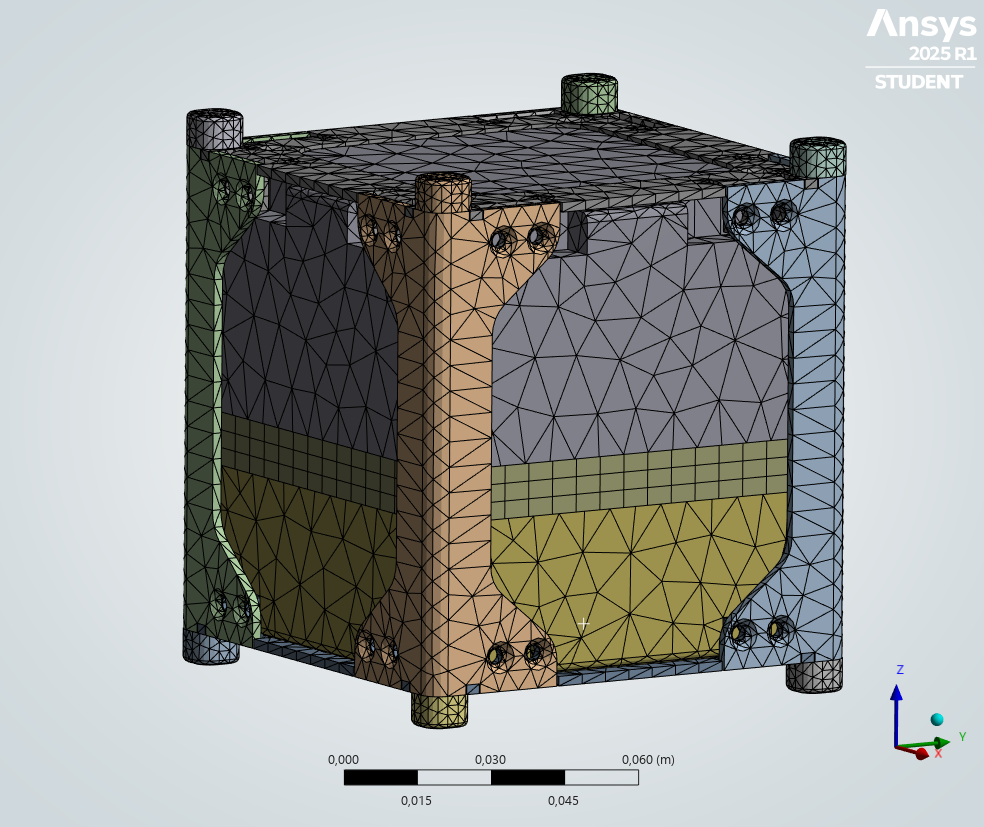
\includegraphics[width=0.7\textwidth]{image/fem/ansys_cubesat-mesh.png}
        \caption{Malla generada automáticamente por ANSYS Mechanical}
        \label{fig:fem_mesh}
      \end{figure}

    \subsubsection{Análisis Modal}

      Para poder proceder a las simulaciones de vibraciones aleatorias (workmanship) y análisis de integridad
      estructural, es necesario determinar las frecuencias modales del CubeSat. En el Cuadro \ref{tab:modos_obtenidos}
      se pueden ver las frecuencias modales encontradas desde 0Hz hasta 2200Hz.

      \begin{table}[H]
      \centering
      \begin{tabular}{|c|c|c|c|c|c|c|}
      \hline
      \textbf{Modo}       & 1           & 2           & 3           & 4         & 5           & 6          \\
      \hline
      \textbf{Frecuencia} & $536.89\,Hz$ & $541.52\,Hz$ & $908.97\,Hz$ & $1253\,Hz$ & $1616.2\,Hz$ & $1624.1\,Hz$ \\
      \hline
      \end{tabular}
      \caption{Modos obtenidos.}
      \label{tab:modos_obtenidos}
      \end{table}

    \subsubsection{Análisis de Vibraciones Aleatorias}

      En este análisis, se sometió el CubeSat a la curva $G^2/Hz$ recomendada por la competencia. Como ANSYS Mechanical
      ya tiene incorporado el mecanismo para conectar puntos por tramos rectos, la curva resultante tiene que pasar por
      los puntos especificados en el Cuadro \ref{tab:accel}, generando una curva como la de la Figura
      \ref{fig:graph_accel}.

      \begin{figure}[!ht]
        \centering
        \begin{minipage}{0.4\textwidth}
          \centering
          \begin{tabular}{|c|c|}
            \hline
            Frecuencia & Aceleración G \\ \hline
            $20 \, Hz$ & $0.01 \, G^2/Hz$ \\ \hline
            $80 \, Hz$ & $0.04 \, G^2/Hz$ \\ \hline
            $500 \, Hz$ & $0.04 \, G^2/Hz$ \\ \hline
            $2000 \, Hz$ & $0.01 \, G^2/Hz$ \\ \hline
          \end{tabular}
          \captionof{table}{Puntos de aceleraciones G según frecuencia.}
          \label{tab:accel}
        \end{minipage}
        \hspace{0.05\textwidth}
        \begin{minipage}{0.4\textwidth}
          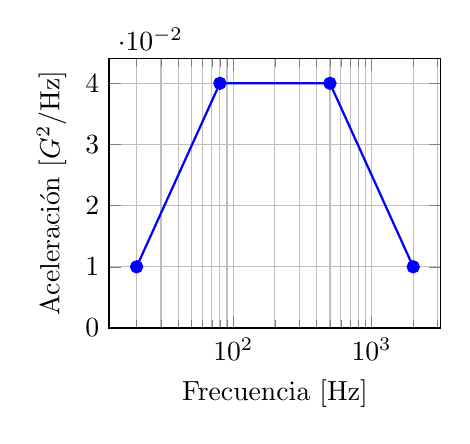
\begin{tikzpicture}
            \begin{axis}[
              xmode=log,
              xlabel={Frecuencia [Hz]},
              ylabel={Aceleración [$G^2$/Hz]},
              grid=both,
              ymin=0,
              height=5cm,
            ]
              \addplot[
                color=blue,
                mark=*,
                thick
              ] coordinates {
                (20, 0.01)
                (80, 0.04)
                (500, 0.04)
                (2000, 0.01)
              };
            \end{axis}
          \end{tikzpicture}
          \caption{Curva con los puntos interpolados de aceleración G.}
          \label{fig:graph_accel}
        \end{minipage}
      \end{figure}

      Esta curva se aplica a los tres ejes del CubeSat, lo que permite generar los análisis de estrés y tensión.

      \begin{figure}[H]
        \begin{minipage}{0.5\textwidth}
          \centering
          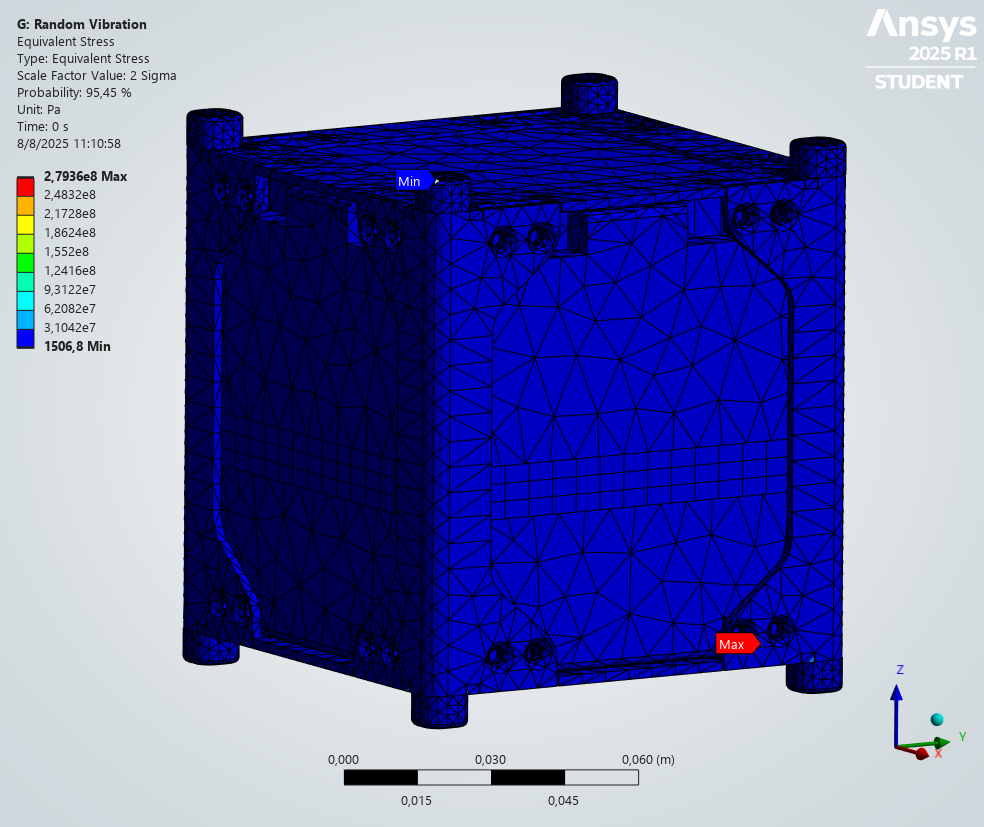
\includegraphics[width=\textwidth]{image/fem/ansys_cubesat-vibration_stress.png}
          \caption{Análisis de estrés}
          \label{fig:fem_stress}
        \end{minipage}
        \hfill
        \begin{minipage}{0.5\textwidth}
          \centering
          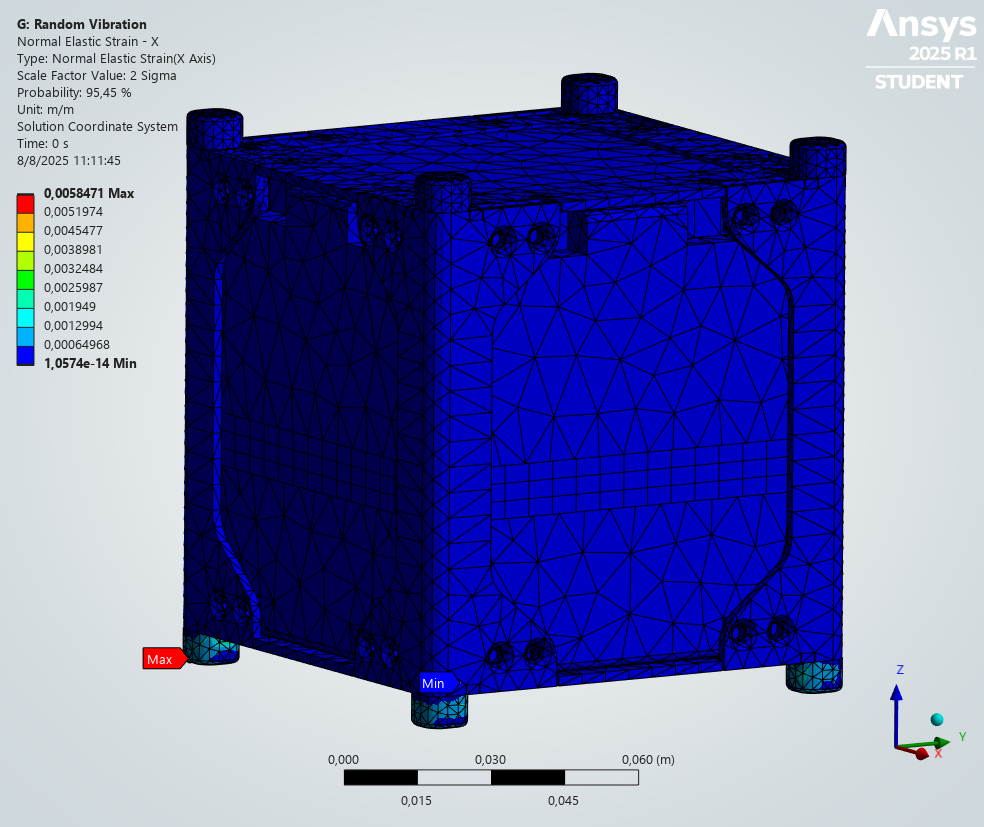
\includegraphics[width=\textwidth]{image/fem/ansys_cubesat-vibration_strain-x.png}
          \caption{Análisis de tensión en el eje Z}
          \label{fig:fem_strain-x}
        \end{minipage}
      \end{figure}
      \begin{figure}[H]
        \begin{minipage}{0.5\textwidth}
          \centering
          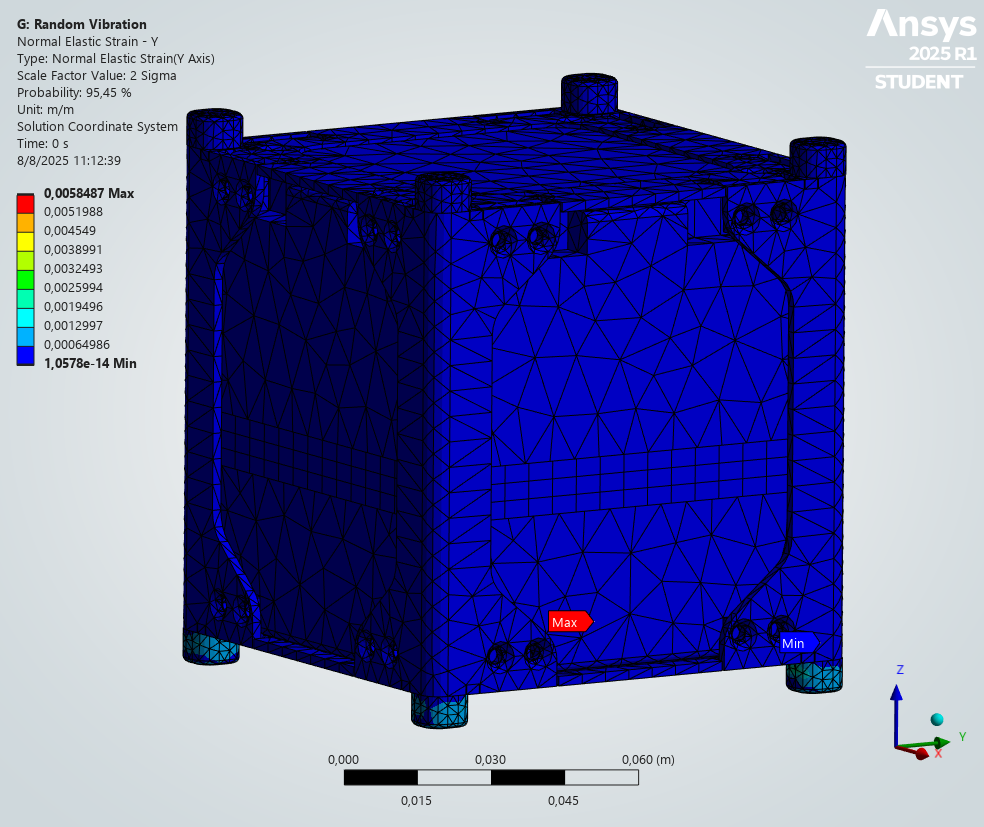
\includegraphics[width=\textwidth]{image/fem/ansys_cubesat-vibration_strain-y.png}
          \caption{Análisis de tensión en el eje Y}
          \label{fig:fem_strain-y}
        \end{minipage}
        \hfill
        \begin{minipage}{0.5\textwidth}
          \centering
          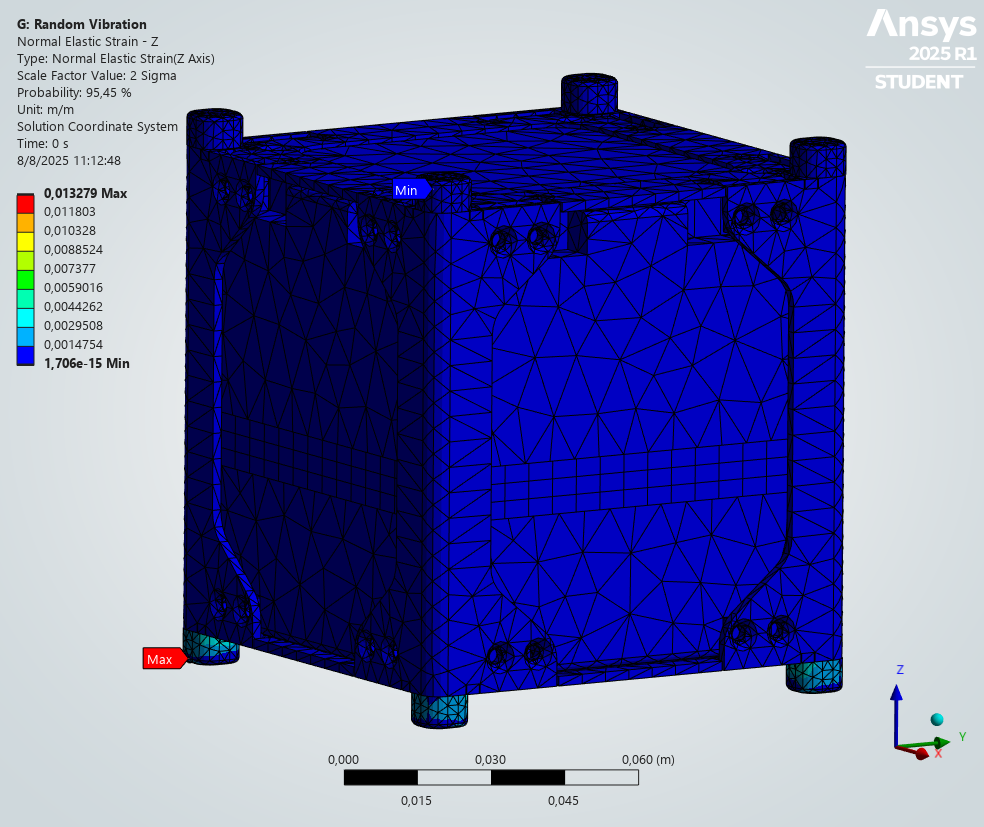
\includegraphics[width=\textwidth]{image/fem/ansys_cubesat-vibration_strain-z.png}
          \caption{Análisis de tensión en el eje Z}
          \label{fig:fem_strain-z}
        \end{minipage}
      \end{figure}

      Como se puede ver en la Figura \ref{fig:fem_stress}, para el análisis de estrés equivalente, el pico máximo es de
      $108.106 \, Pa$. Analizando con más detalle, este punto se encuentra en la superficie de contacto de la tapa
      inferior y la varilla. Debido al límite de resolución, este punto de alta presión puede ser una falla de
      simulación, pero en caso de que no lo sea, sigue estando por debajo del límite de rotura del aluminio y del acero,
      por lo que no presenta un problema.

    \subsubsection{Análisis Estático}
    \begin{minipage}{\textwidth}
      \begin{wrapfigure}{R}{0.4\textwidth}
        \vspace{-0.5cm}
        \centering
        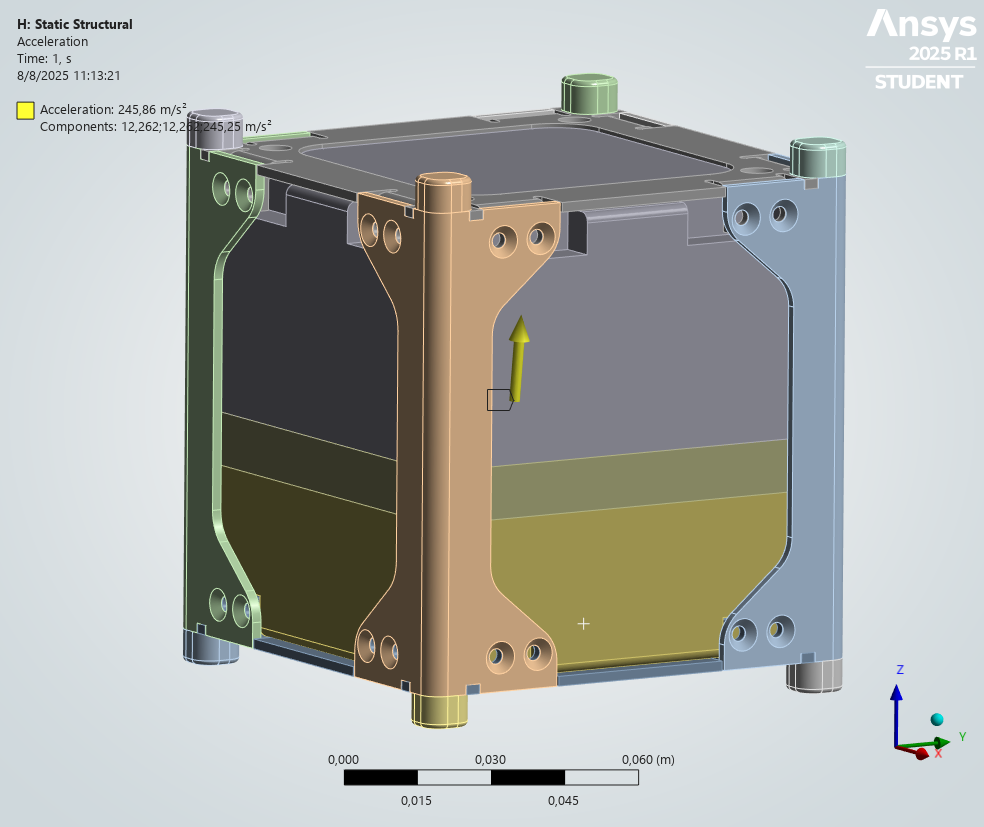
\includegraphics[width=0.33\textwidth]{image/fem/ansys_cubesat-static_acceleration.png}
        \caption{Vector de aceleración para la simulación estática.}
        \label{fig:fem_static_acc}
      \end{wrapfigure}

      \hspace*{1em} Se espera que el CubeSat esté sometido a unas aceleraciones de hasta 20G en el sentido +z y hasta 1G en los
      sentidos x e y. Para las simulaciones, se utilizaron estos valores con un factor de 1.25x. Un detalle que cabe
      destacar, es que todas las deformaciones presentes en estas simulaciones, están amplificadas visualmente para
      facilitar la detección patrones y fallas en el diseño de la estructura, por lo tanto, es fundamental interpretar
      los resultados en función de las escalas de color y los valores numéricos de los distintos análisis, y no tomar
      como referencia la magnitud visual de las deformaciones mostradas. Aclarado esto, se muestran a continuación las
      simulaciones realizadas.
    \end{minipage}

      \begin{figure}[H]
        \begin{minipage}{0.5\textwidth}
          \centering
          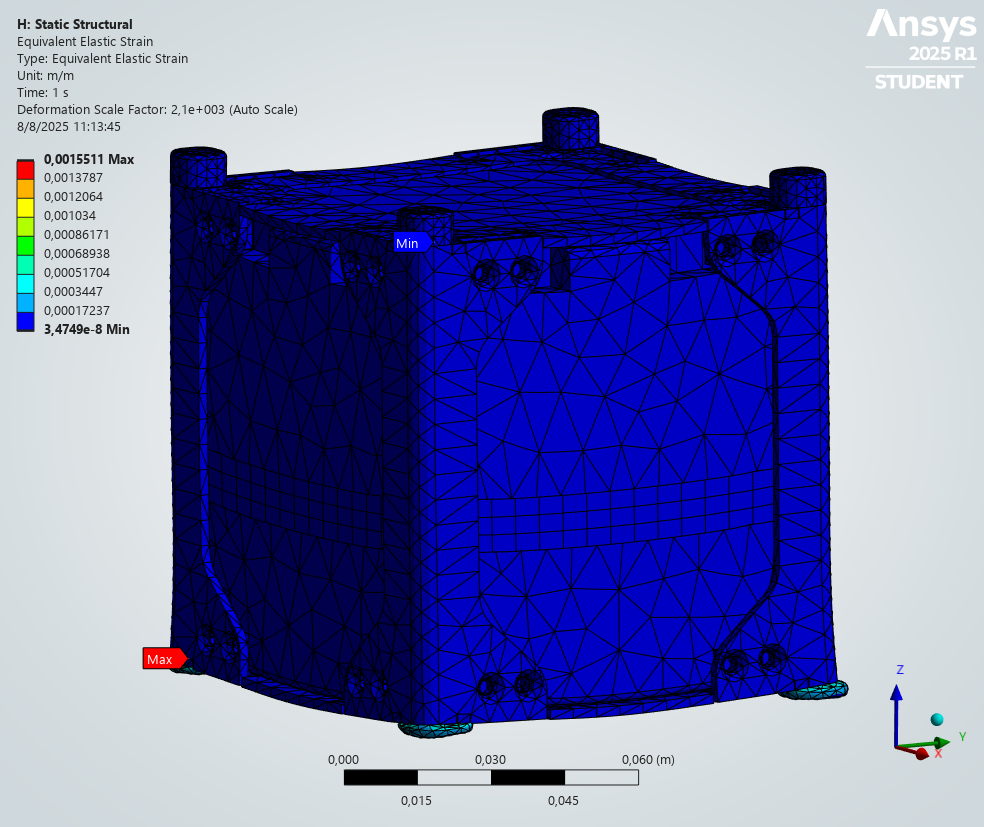
\includegraphics[width=\textwidth]{image/fem/ansys_cubesat-static_strain.png}
          \caption{Análisis de tensión}
          \label{fig:fem_static_strain}
        \end{minipage}
        \hfill
        \begin{minipage}{0.5\textwidth}
          \centering
          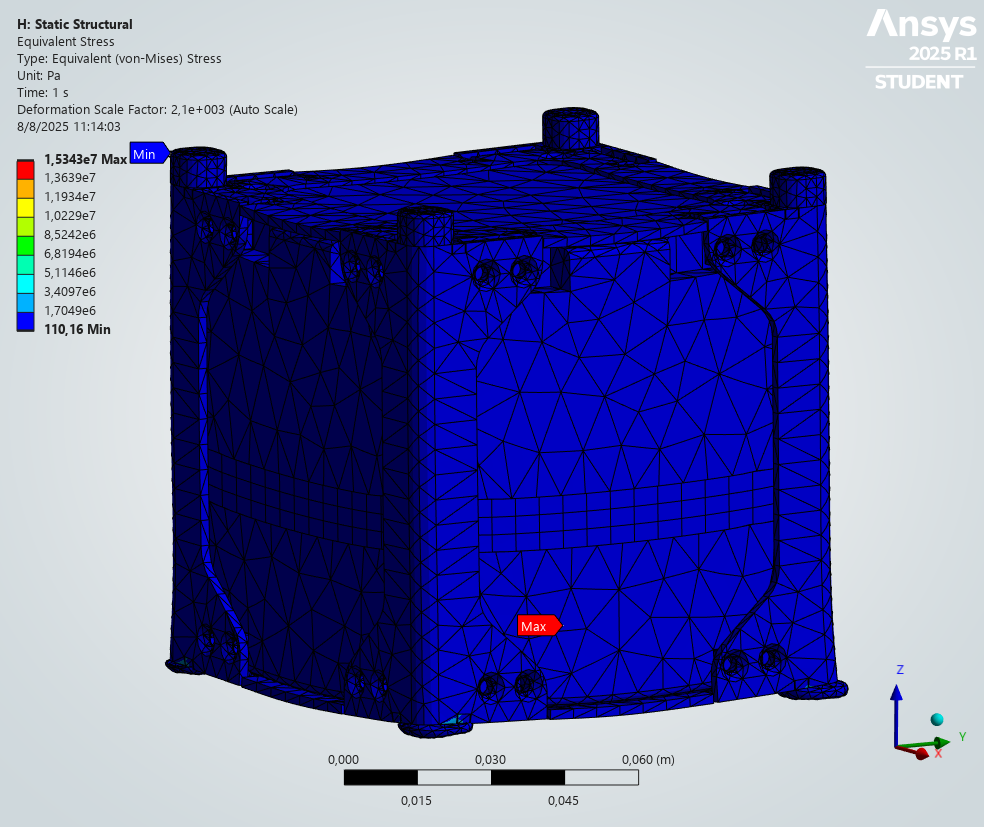
\includegraphics[width=\textwidth]{image/fem/ansys_cubesat-static_stress.png}
          \caption{Análisis de estrés}
          \label{fig:fem_static_stress}
        \end{minipage}
      \end{figure}
      \begin{figure}[H]
        \begin{minipage}{0.5\textwidth}
          \centering
          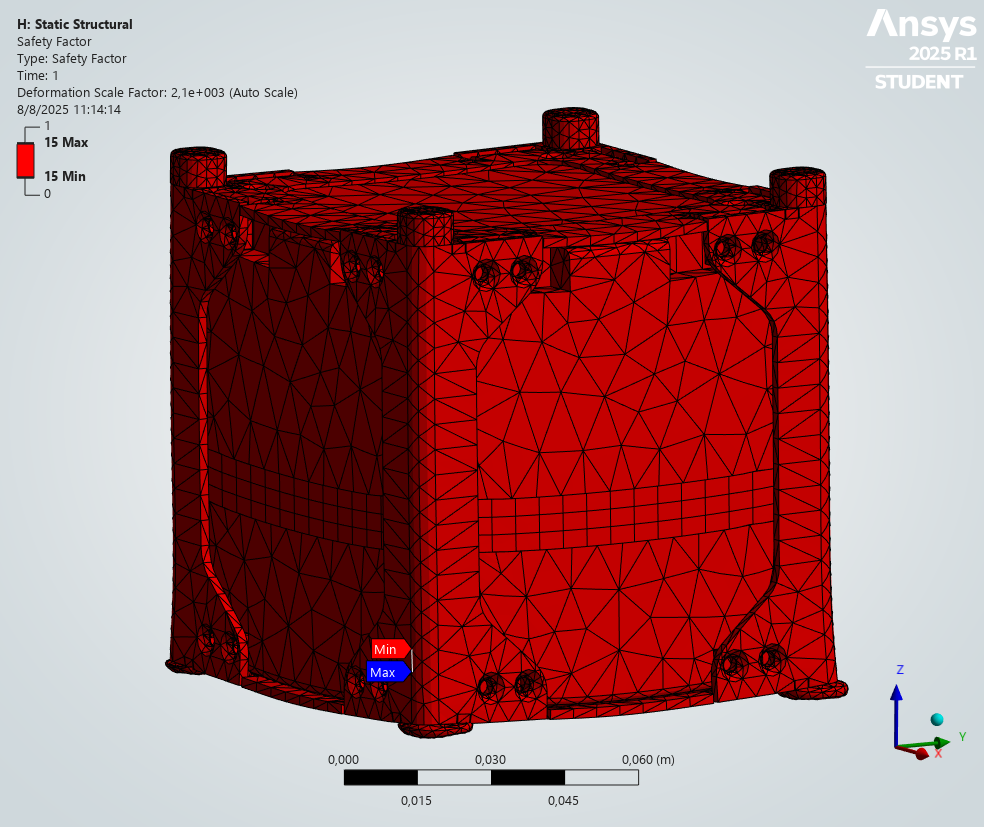
\includegraphics[width=\textwidth]{image/fem/ansys_cubesat-static_safety.png}
          \caption{Análisis de factor de seguridad}
          \label{fig:fem_static_safety}
        \end{minipage}
        \hfill
        \begin{minipage}{0.5\textwidth}
          \centering
          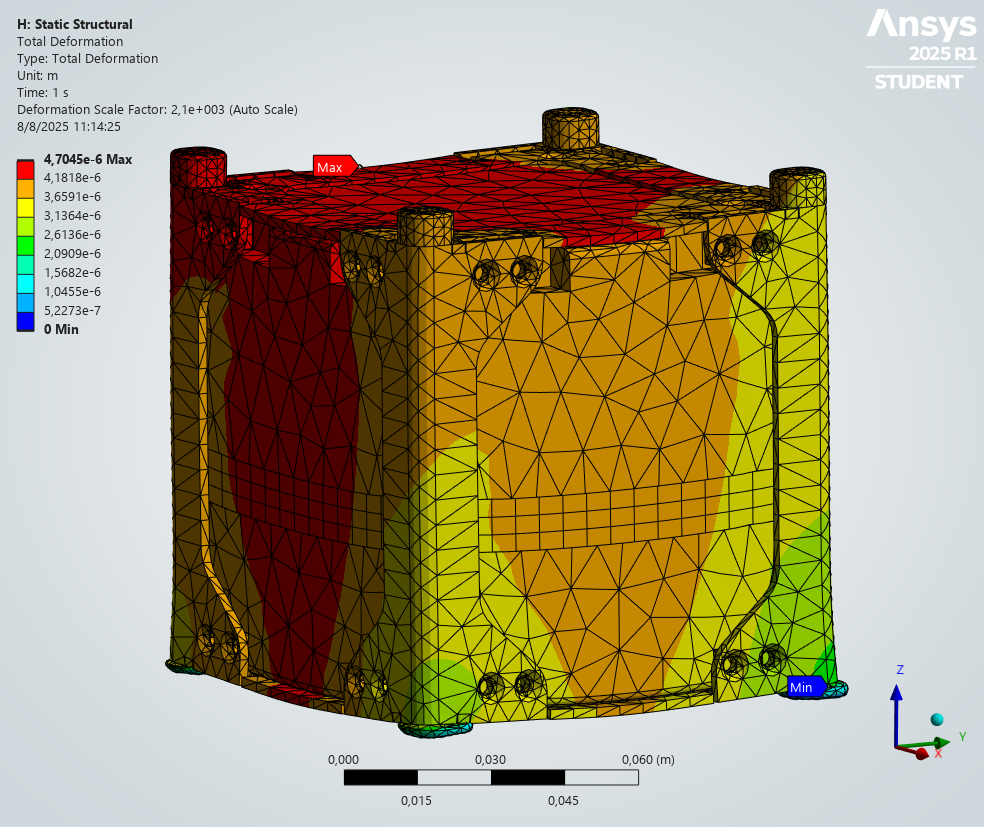
\includegraphics[width=\textwidth]{image/fem/ansys_cubesat-static_deformation.png}
          \caption{Análisis de deformación total}
          \label{fig:fem_static_deformation}
        \end{minipage}
      \end{figure}

      Como se observa en la Figura \ref{fig:fem_static_strain}, la tensión máxima alcanzada en la estructura es de
      $19.106 \, Pa$, valor significativamente inferior al límite de rotura del material, lo que indica que no existe
      riesgo estructural bajo las condiciones de carga previstas para el lanzamiento. Asimismo, la Figura
      \ref{fig:fem_static_safety} muestra que el factor de seguridad es uniforme en toda la estructura y alcanza un
      valor constante de 15, lo cual proporciona un amplio margen respecto a posibles fallos. Finalmente, según la
      Figura \ref{fig:fem_static_deformation}, la deformación máxima experimentada por el CubeSat es de apenas $4\um$,
      lo cual resulta despreciable frente a las tolerancias mecánicas del sistema.

      Concluimos entonces que nuestra propuesta de estructura es válida y soportara las condiciones de lanzamiento.

  \subsection{Análisis de Riesgos}
    En esta sección se presenta un análisis de riesgos para los subsistemas del CubeSat, utilizando una metodología de
    matriz de riesgo de 5x5. Este enfoque asigna un nivel de severidad y una probabilidad de ocurrencia a cada evento
    potencial, permitiendo una priorización clara de las estrategias de mitigación.
  
  \subsubsection{Escala de severidad}
  \begin{enumerate}[label=\textbf{\arabic*.}]
    \item \textbf{Insignificante:} Su ocurrencia genera consecuencias que no afectan el funcionamiento del sistema ni
      comprometen los objetivos del proyecto.
    \item \textbf{Menor:} Puede causar pequeñas pérdidas, pero sus consecuencias son fácilmente gestionables.
    \item \textbf{Moderada:} Genera un impacto considerable que requerirá de tiempo y demás recursos para ser
      solucionado.
    \item \textbf{Importante:} Las consecuencias requieren intervención inmediata porque pueden causar daños a largo
      plazo, afectando seriamente el cumplimiento de objetivos.
    \item \textbf{Catastrófica:} El impacto es crítico. Las consecuencias ponen en riesgo la viabilidad del proyecto o
      generan grandes pérdidas.
  \end{enumerate}
  
  \subsubsection{Escala de probabilidad}
  \begin{enumerate}
    \item \textbf{Muy baja:} Ocurrencia casi imposible.
    \item \textbf{Baja:} Podría ocurrir, pero sería extraño.
    \item \textbf{Media:} Puede ocurrir ocasionalmente.
    \item \textbf{Alta:} Casi seguro que suceda.
    \item \textbf{Muy alta:} Podemos dar por hecho que sucederá.
  \end{enumerate}

  \begin{table}[H]
\centering
\scriptsize
\begin{tabular}{|p{2cm}|p{2cm}|p{2cm}| p{2cm} |p{2cm}| p{2cm}|}
\hline \bf Probabilidad/ Severidad & \bf 1-Muy baja & \bf 2-Baja & \bf 3-Media & \bf 4-Alta & \bf 5-Muy alta\\ [10pt]

\hline \bf 5-Catastrófico & \cellcolor{yellow!50} & \cellcolor{red!50} & \cellcolor{red!50} & \cellcolor{red!50} &\cellcolor{red!50} \\ [10pt]

\hline \bf 4-Importante & \cellcolor{yellow!50} & \cellcolor{yellow!50} & \cellcolor{red!50} & \cellcolor{red!50} &\cellcolor{red!50} \\ [10pt]

\hline \bf 3-Moderada &\cellcolor{green!50} & \cellcolor{yellow!50} & \cellcolor{yellow!50} & \cellcolor{red!50} &\cellcolor{red!50} \\ [10pt]

\hline \bf 2-Menor & \cellcolor{green!50} & \cellcolor{green!50} & \cellcolor{yellow!50} &\cellcolor{yellow!50} &\cellcolor{red!50} \\ [10pt]

\hline \bf 1-Insignificante & \cellcolor{green!50} & \cellcolor{green!50} & \cellcolor{green!50} &\cellcolor{yellow!50} &\cellcolor{yellow!50} \\ [10pt]
\hline
\end{tabular} \\
\caption{Matriz de riesgo}
\end{table}
  
  \subsubsection{Impacto del riesgo}
    Se calcula multiplicando la severidad y la probabilidad de cada riesgo.


\begin{table}[H]
\centering
%\scriptsize
\begin{tabular}{|p{1.5cm}|p{13cm}|}
\hline \bf Color & \bf Descripción \\
\hline \cellcolor{red! 50} & Su mitigación es prioritaria. Comprometen el exito de la mision \\ [10pt]
\hline \cellcolor{yellow! 50} & Deben revisarse para implementar estrategias de mejora. \\[10pt]
\hline \cellcolor{green! 50} & Ocurrencia poco probable. Pueden considerarse para un análisis más detallado. \\ [10pt]
\hline
\end{tabular}
\caption{Impacto del riesgo}
\end{table}

   \begin{table}[H]
    \centering
    \resizebox{\textwidth}{!}{
    \begin{tabular}{ | m{3.5cm} | m{3.5cm} | m{3.5cm} | m{5cm} | m{2cm} | }
      \hline
      \textbf{Riesgo} & \textbf{Causa} & \textbf{Consec.} & \textbf{Mitigación} & \textbf{Impacto: P/S} \\
      \hline
      Rotura de cápsulas de muestras & Sobrecargas mecánicas o vibraciones excesivas & Pérdida parcial o total de las muestras biológicas & Análisis FEM de su portador, ensayos y rediseño en caso de ser necesario. & \cellcolor{yellow! 50} 1/5\\ 
      \hline
      Fallo del sistema de regulación térmica & Mal dimensionamiento de los elementos Peltier o fallo de controlador en vuelo. & Exposición de muestras a temperaturas fuera de rango. & Ensayos apropiados de capacidad calorífica y consumo energético. & \cellcolor{yellow! 50} 3/3\\
      \hline
      Pérdida de datos por fallo de almacenamiento & Corrupción de tarjeta microSD o falla en conmutación RAID por script. & Pérdida parcial o total de registros de muestras. & Verificación periódica de integridad. Script de conmutación automática. Redundancia de almacenamiento de datos críticos. & \cellcolor{red! 50} 2/5\\
      \hline
      Fallo del suministro eléctrico & Sobrecarga de rieles, cortocircuito o desconexión no deseada. & Apagado de subsistemas. & Ensayos en fases de prueba y rediseño en caso de ser necesario. Rieles críticos alimentados desde canales independientes. & \cellcolor{red! 50} 2/5\\
      \hline
      Mal funcionamiento de la IMU o barómetro & Descalibración por choque mecánico o ruido eléctrico. & Imposibilidad de determinar fases de vuelo con precisión. & Pruebas previas en condiciones similares. &\cellcolor{yellow! 50} 1/4\\
      \hline
      Contaminación o degradación de muestras biológicas & Fugas de medios de cultivo, exposición al ambiente. & Resultados experimentales no válidos, pérdida de muestras. & Sellado hermético de tubos. & \cellcolor{yellow! 50} 1/4\\
      \hline
      Fallo de comunicación pos lanzamiento & Rotura de hardware en aterrizaje o vuelo. & Imposibilidad de monitoreo inmediato luego del lanzamiento. & Múltiples opciones de conexión. & \cellcolor{yellow! 50} 2/3\\
      \hline
    \end{tabular}
    }
    \caption{Análisis de Riesgos}
    \label{tab:analisis-riesgos}
  \end{table}

  \subsection{Plan de Verificación y Ensayos}
    En esta sección se detallan los ensayos que se realizarán a los distintos prototipos que surgirán durante él
    desarrollo del CubeSat, que servirán para validar y obtener una retroalimentación del proceso de diseño.

    \subsubsection{Estructura}
      Para determinar la integridad estructural se realizarán distintos tipos de pruebas, donde las condiciones de cada
      una serán acordes a las del lanzamiento, y también se realizarán pruebas extremas, para encontrar los límites de
      la estructura y poder ampliar el margen de seguridad. Para lograr esto, se realizarán varias estructuras, y sé las
      rellenará con subsistemas vacíos pero con el peso necesario para llegar al régimen.

      Las pruebas que se realizarán a la estructura son:
      \begin{itemize}
        \item Prueba de vibraciones: Se somete el prototipo a una cama de vibraciones para determinar si se mantiene en
          forma durante todo el rango de frecuencias y más.
        \item Prueba de caída: Se somete el prototipo a pruebas de caída de diferentes alturas y buscando que impacte en
          diferentes puntos de la estructura para probar la rigidez estructural y capacidad de contención de las
          carcasas de los subsistemas.
        \item Prueba de fuerzas: Se somete el prototipo a fuerzas (que ingresan y egresan a la estructura) ejercidas en
          puntos críticos donde las tensiones pueden alcanzar picos y generar deformaciones.
      \end{itemize}
    \subsubsection{Peso}
      Para determinar que el CubeSat se encuentra dentro del régimen, a medida que se vayan haciendo los diferentes
      prototipos, se pesará todo el CubeSat que se tenga hasta el momento para tener estimaciones más precisas de peso, y
      poder llegar con el margen de tolerancias especificado sin tener que hacer cambios grandes.

    \subsubsection{Centro de masa}
      Para determinar experimentalmente el centro de masa del CubeSat, colocamos una madera rectangular de espesor
      mínimo sobre una superficie plana, de modo que el lado más estrecho y largo se encuentre en contacto con la
      superficie. Arriba colocamos el CubeSat formando 4 ángulos rectos, es decir que las direcciones sus aristas sean
      paralelas y perpendiculares a la dirección de la madera. Deslizamos el CubeSat horizontalmente hasta encontrar un
      punto de equilibrio, esa será la coordenada del centro de masa en ese eje. Repetimos el procedimiento para los
      demás ejes y verificamos, en cada caso, que se encuentren a una distancia del centro geométrico de a lo sumo 10
      mm.

    \subsubsection{Baterías}
      \begin{itemize}
        \item \textbf{Capacidad real:} este ensayo tiene como finalidad determinar la capacidad efectiva de la batería,
          comparándola con la especificación nominal del fabricante. Para ello, se descargará la batería con una
          corriente constante conocida hasta alcanzar el voltaje mínimo especificado. Se registrará el tiempo total de
          descarga para calcular la capacidad en mAh.  El resultado permitirá verificar si la batería puede sostener la
          demanda energética del sistema durante el tiempo requerido.

        \item \textbf{Medición de voltaje y corriente durante carga y descarga:} Durante las fases de carga y descarga,
          se monitorearán de forma continua los valores de tensión y corriente entregados por la batería. Esto permitirá
          evaluar la estabilidad de las baterías frente a distintas condiciones de carga, así como detectar caídas de tensión
          o comportamientos no deseados que puedan comprometer la operación de los subsistemas.

        \item \textbf{Medición de temperatura:} durante los ensayos anteriores se registrará también la evolución
          térmica de la batería. Esto permitirá identificar posibles sobrecalentamientos que puedan comprometer la
          seguridad o el rendimiento del sistema.
      \end{itemize}

    \subsubsection{Electrónica}
      Para hacer una prueba a la electrónica, se conectarán las placas afuera del CubeSat, para poder conectarlas
      a una fuente de alimentación externa. Con la fuente externa podemos:
      \begin{itemize}
        \item \textbf{Monitorear el consumo del CubeSat:} con condiciones preestablecidas, se puede comparar si los
          consumos son acordes a los estimados y si la medición está dentro de los márgenes de error establecidos.
        \item \textbf{Comparar lecturas con mediciones:} Se puede acceder a la \acrshort{pms} para medir los voltajes de
          las fuentes de salida y compararlos con los reportados por la misma en la interfaz web.
        \item \textbf{Pruebas intensivas de las fuentes:} Para encontrar los límites operativos y ver si las
          protecciones implementadas funcionan correctamente.
        \item \textbf{Prueba de estabilidad de programa:} Involucra dejar el CubeSat en modo lanzamiento por un periodo
          prolongado (por lo menos 4 veces el tiempo de misión máximo) para corroborar que los programas sean estables y
          no generen corrupción ni perdida de datos.
      \end{itemize}

    \subsubsection{Transferencia térmica}
      Se ensamblara el CubeSat y se colocaran muestras de agua para probar la capacidad de disipación y transferencia
      térmica de las celdas Peltier. Asimismo, se verificará que los cambios de temperatura no signifiquen un problema
      para la estructura plástica. Por otro lado, se validará el sistema de disipación pasivo para las celdas Peltier.

\section{Plan de Proyecto}

  \subsection{General}
    Para llevar a cabo la misión del CubeSat, se ha definido una estructura de trabajo que
    divide al equipo en diferentes grupos, cada uno con responsabilidades específicas. Esta división
    busca optimizar el desarrollo del proyecto mediante una organización eficiente de tareas y
    recursos humanos.
    \subsubsection{Organización del Equipo}
      \begin{itemize}
        \item \textbf{Project Manager (PM)}
          Coordinador general del proyecto, responsable de la planificación y del funcionamiento
          sincronizado de todos los grupos y subsistemas.
          \begin{itemize}
            \item Cortesini Perez, Luciano Tomas
          \end{itemize}
        \item \textbf{Grupo Mecánico}
         Encargado del diseño estructural del CubeSat.
          \begin{itemize}
            \item Cortesini Perez, Luciano Tomas
            \item Palombo, Franco
          \end{itemize}
        \item \textbf{Grupo Electrónica}
          Responsable del diseño, desarrollo y pruebas de los subsistemas electrónicos, incluyendo
          potencia y sensores.
          \begin{itemize}
            \item Gil, Ignacio
            \item Prieto, Angelo
            \item Palombo, Franco
          \end{itemize}
          \item \textbf{Grupo Software}
          Encargado del desarrollo del software tanto embarcado como de recuperación y procesamiento de datos.
          \begin{itemize}
            \item Koroch, Matias Adolfo
            \item Montesinos, Dana Carolina
          \end{itemize}
        \item \textbf{Grupo de Divulgación}
          Consideramos valioso compartir los trabajos que se llevan a cabo en nuestra facultad para
          visibilizar el trabajo académico, motivar a otros estudiantes, reconocer el valor de la investigación
          científica como as también crear puentes entre la universidad y la sociedad. No solo buscamos cumplir con los
          objetivos técnicos y científicos de la misión, sino también inspirar y promover el interés por la ciencia en
          la comunidad de nuestra región.

          Se buscará documentar las distintas etapas del proyecto registrando con
          fotos y vídeos, generando informes y difundiendo hacia la comunidad por medio de distintas plataformas y redes
          sociales, principalmente Instagram.

          Además con el propósito de consolidar la transparencia, fomentar la comunicación científica y promover la apropiación
          social del conocimiento generado por el Proyecto CubeSat LAMBDA, se ha proyectado el desarrollo de una plataforma
          web pública de documentación y divulgación, dirigida tanto a la comunidad académica como al público general. Este
          portal actuará como repositorio centralizado de información técnica y divulgativa, posibilitando la consulta
          interactiva, el seguimiento del progreso de la misión y el acceso a documentación validada.
        \end{itemize}
 
  \subsection{Cronograma}
    Con el objetivo de garantizar una ejecución ordenada, eficiente y dentro de los plazos establecidos, se elaboró un
    cronograma detallado para cada uno de los grupos de trabajo que contempla las diferentes tareas ha realizar junto
    con los diferentes fechas y plazos estipulados para cada una de ellas.

    Utilizamos una herramienta basada en diagramas Gantt de gestión estratégica para lograr visualizar con facilidad la
    secuencia lógica de actividades, sus respectivas duraciones, y las dependencias entre tareas.

    Para el desarrollo de este proceso se tuvieron en cuenta distintas variables como las fechas límites, los objetivos
    planteados, la disponibilidad de tiempo, los recursos económicos y el capital humano.

    \subsubsection{Grupo Mecánico}
    Para una visualización del cronograma, se remite al diagrama Gantt incluido en el anexo, Figura
    \ref{gantt-mecanica1} y Figura \ref{gantt-mecanica2}.
    \subsubsection{Grupo Electrónica}
    Para una visualización del cronograma, se remite al diagrama Gantt incluido en el anexo, Figura
    \ref{gantt-hardware}.
    \subsubsection{Grupo Software}
    Para una visualización del cronograma, se remite al diagrama Gantt incluido en el anexo.
  \subsection{Costos y Financiamiento}

  La validación de los requerimientos funcionales y operacionales del CubeSat requiere la disponibilidad de insumos,
  herramientas, equipamiento e infraestructura adecuada que permitan llevar a cabo pruebas técnicas rigurosas. En este
  sentido, la presente sección contempla la financiación necesaria para la adquisición de los materiales e instrumentos
  que permitan fabricar el CubeSat, así como realizar los ensayos pertinentes para el cumplimiento de las
  especificaciones establecidas.

  La financiación prevista abarca los siguientes componentes:

  \begin{itemize}
    \item \textbf{Adquisición de insumos}: incluye sensores, microcontroladores, estructuras mecánicas, módulos de
      almacenamiento, elementos de conexión y otros componentes electrónicos y estructurales necesarios para la
      fabricación del CubeSat.

    \item \textbf{Herramientas de validación y ensayo}: contempla equipamiento de medición, dispositivos de prueba
      funcional, sistemas de monitoreo térmico y mecánico, así como herramientas de ensamblaje y diagnóstico utilizadas
      durante las etapas de verificación.

    \item \textbf{Acceso a infraestructura y servicios}: incluye la utilización de laboratorios y bancos de prueba. En
      particular, se destaca el acceso a las instalaciones del \textit{Centro de Investigación en Informática para la
      Ingeniería (CIII)} y del \textit{Instituto de Investigación Médica Mercedes y Martín Ferreyra
      (INIMEC-CONICET-UNC)}, los cuales proporcionan equipamiento especializado, condiciones técnicas adecuadas y
      asesoramiento científico para la ejecución de los ensayos requeridos.

  \end{itemize}

  Los recursos económicos serán obtenidos a través del respaldo de personas, grupos o instituciones interesadas en
  promover la investigación científica y tecnológica del proyecto. Asimismo, se aprovecharán los recursos
  institucionales disponibles dentro del marco académico. Cualquier interesado puede donar al proyecto mediante la
  página web detallada en la Sección \ref{sec:paginaweb}.

  \begin{table}[H]
    \centering
    \begin{tabular}{|l|r|r|r|}
      \hline
      \textbf{Item} & \textbf{Cantidad} & \textbf{Precio} & \textbf{Subtotal} \\
      \hline
      RPI Zero 2W                                     & 1     & 36299   & 36299 \\
      Micro SD 16GB                                   & 2     & 13619   & 27238 \\
      Arduino NANO                                    & 1     & 6190    & 6190  \\
      Modulo MP1584                                   & 3     & 3100    & 9300  \\
      Puente H L298N                                  & 2     & 5000    & 10000 \\
      Conversor analógico-digital ADS1115             & 2     & 6000    & 12000 \\
      Sensor de corriente INA219                      & 1     & 6000    & 6000  \\
      Plancha de aluminio 2x250x250mm                 & 1     & 7300    & 7300  \\
      Varillas acero 5mm 96mm                         & 4     & 1800    & 7200  \\
      Baterías 18650 CMICR18650-F9L                   & 5     & 15000   & 75000 \\
      Filamento PP-T grilon3                          & 0.5   & 24780   & 12390 \\
      PCB virgen 20x10cm                              & 1     & 6700    & 6700  \\
      Celda Peltier 30x30mm                           & 3     & 18700   & 56100 \\
      Thermistor ntc 100k                             & 4     & 3890    & 15560 \\
      MPU9250 (\acrshort{imu})                        & 1     & 22490   & 22490 \\
      BMP280 (Barómetro)                              & 1     & 2344    & 2344  \\
      Tornillos M3x6mm cabeza Allen fresada           & 78    & 100     & 7800  \\
      Tuercas Nyloc M3                                & 32    & 60      & 1920  \\
      Componentes electrónicos varios                 & 1     & 10000   & 10000 \\
      Tornillería varia                               & 1     & 5000    & 5000  \\
      \hline
      \multicolumn{3}{|r|}{\textbf{Total:}} & \textbf{336831} \\
      \hline
    \end{tabular}
    \caption{Costos}
    \label{tab:costos}
  \end{table}

   \subsection{Estado de insumos}
    Actualmente, hemos adquirido la Raspberry Pi Zero 2 W, que es uno de los componentes centrales y uno de los más
    propensos a dejar de estar disponible y el filamento de Polipropileno. Se presenta una lista de los elementos que
    aún no se han adquirido, pero siguen estando disponibles:
    \begin{itemize}
      \item Celdas Peltier 30x30mm
      \item Puente H L298N
      \item Conversor Analogico-Digital ADS1115
      \item \acrfull{imu} MPU9250
      \item Barometro BMP280
      \item Sensor de Corriente INA219
      \item Arduino Nano
      \item Celdas Li-Ion CMICR18650-F9L
      \item Termistores
      \item Tornilleria
    \end{itemize}

    Algunos elementos no listados ya fueron adquiridos para el prototipo, pero será necesario comprarlos nuevamente
    (chapa de aluminio, varillas, PCB Virgen, etc.). Apenas tengamos la confirmación de clasificación, se comenzará con
    la compra de los elementos a medida que se vayan necesitando en el desarrollo.

\chapter{Información Adicional}

\section{Repositorios}

Uno de los valores fundamentales de este proyecto es su carácter abierto y reutilizable.  Con el objetivo de facilitar
la continuidad, adaptación y mejora del desarrollo por parte de otros equipos o instituciones, todo el trabajo realizado
sera publicado en un repositorio publico en GitHub, bajo la licencia Apache 2.0.

El repositorio incluirá los modelos CAD, esquemáticos, código fuente del software embarcado. Todo con su respectiva
documentación técnica, permitiendo a cualquier interesado acceder de manera completa al diseño del sistema.

Asimismo, se ha procurado que todas las herramientas de software utilizadas durante el desarrollo sean de acceso libre o
cuenten con licencias educativas gratuitas fácilmente accesibles. Garantizando que el uso de herramientas no represente
una barrera de entrada para quienes deseen replicar o continuar el proyecto.

URL del proyecto: \url{https://github.com/Team-COREX}

\pagestyle{empty}
\newgeometry{left=3mm,right=3mm,top=3mm,bottom=3mm,}
\chapter{Anexo}

\section{Página web HMI} \label{anexo:webpage}
  \begin{figure}[H]
    \centering
    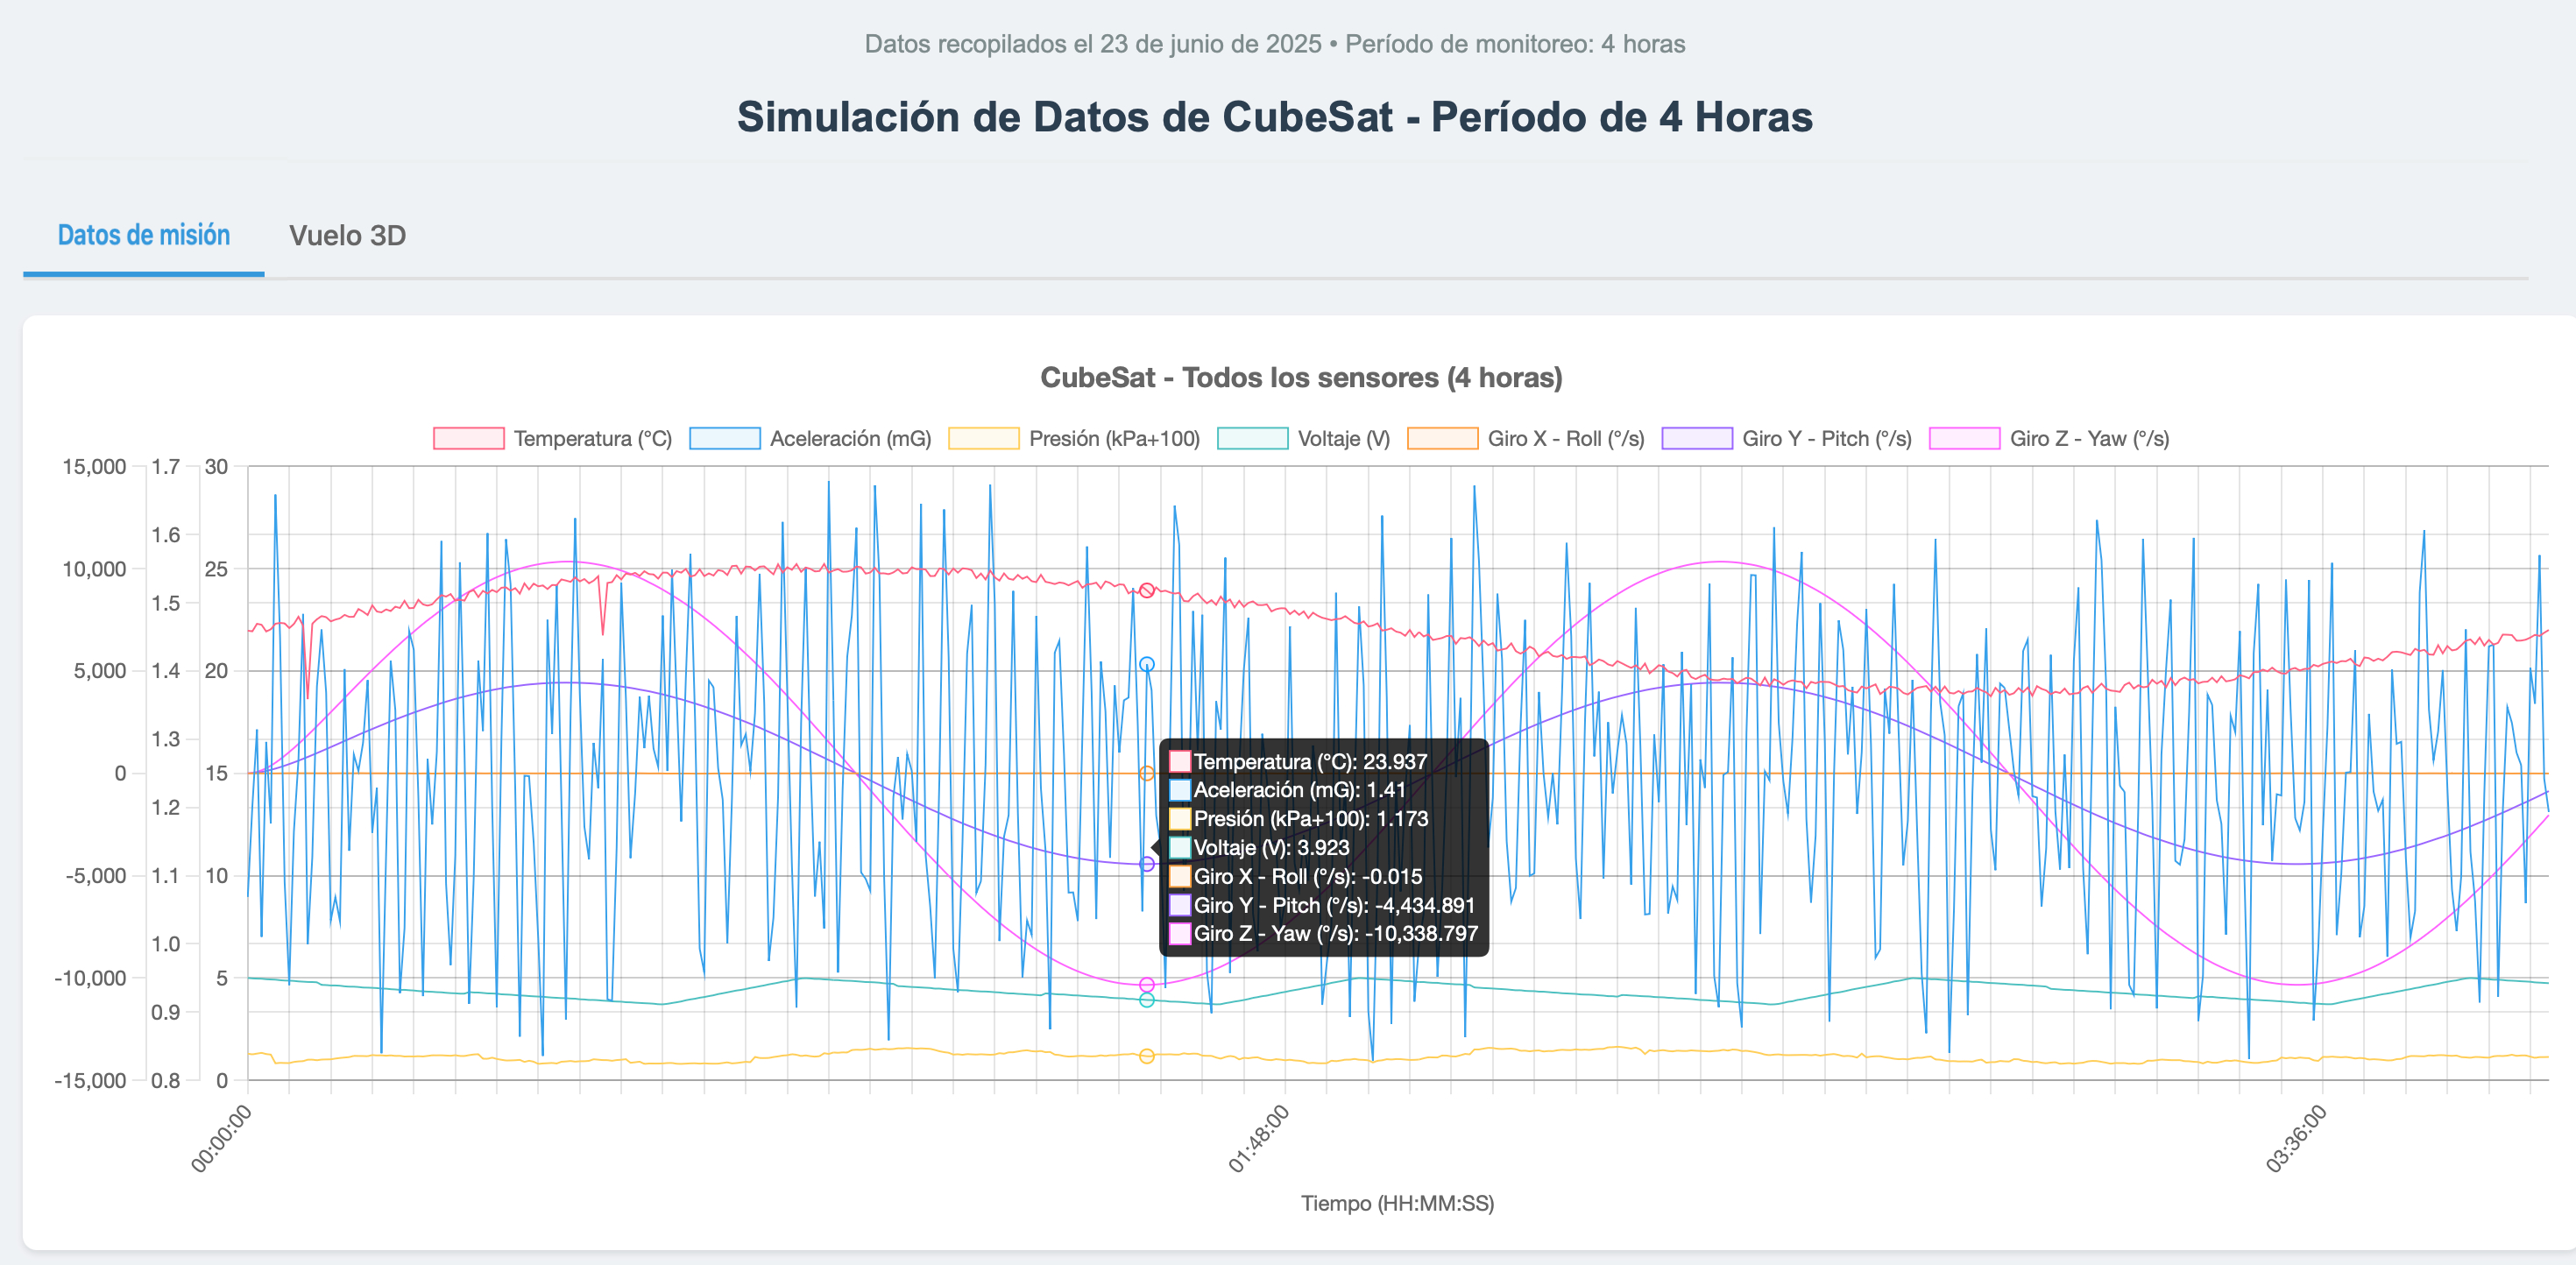
\includegraphics[width=18cm]{image/web/simulacion.jpg}
    \caption{Página Web 1}
  \end{figure}
  \begin{figure}[H]
    \centering
    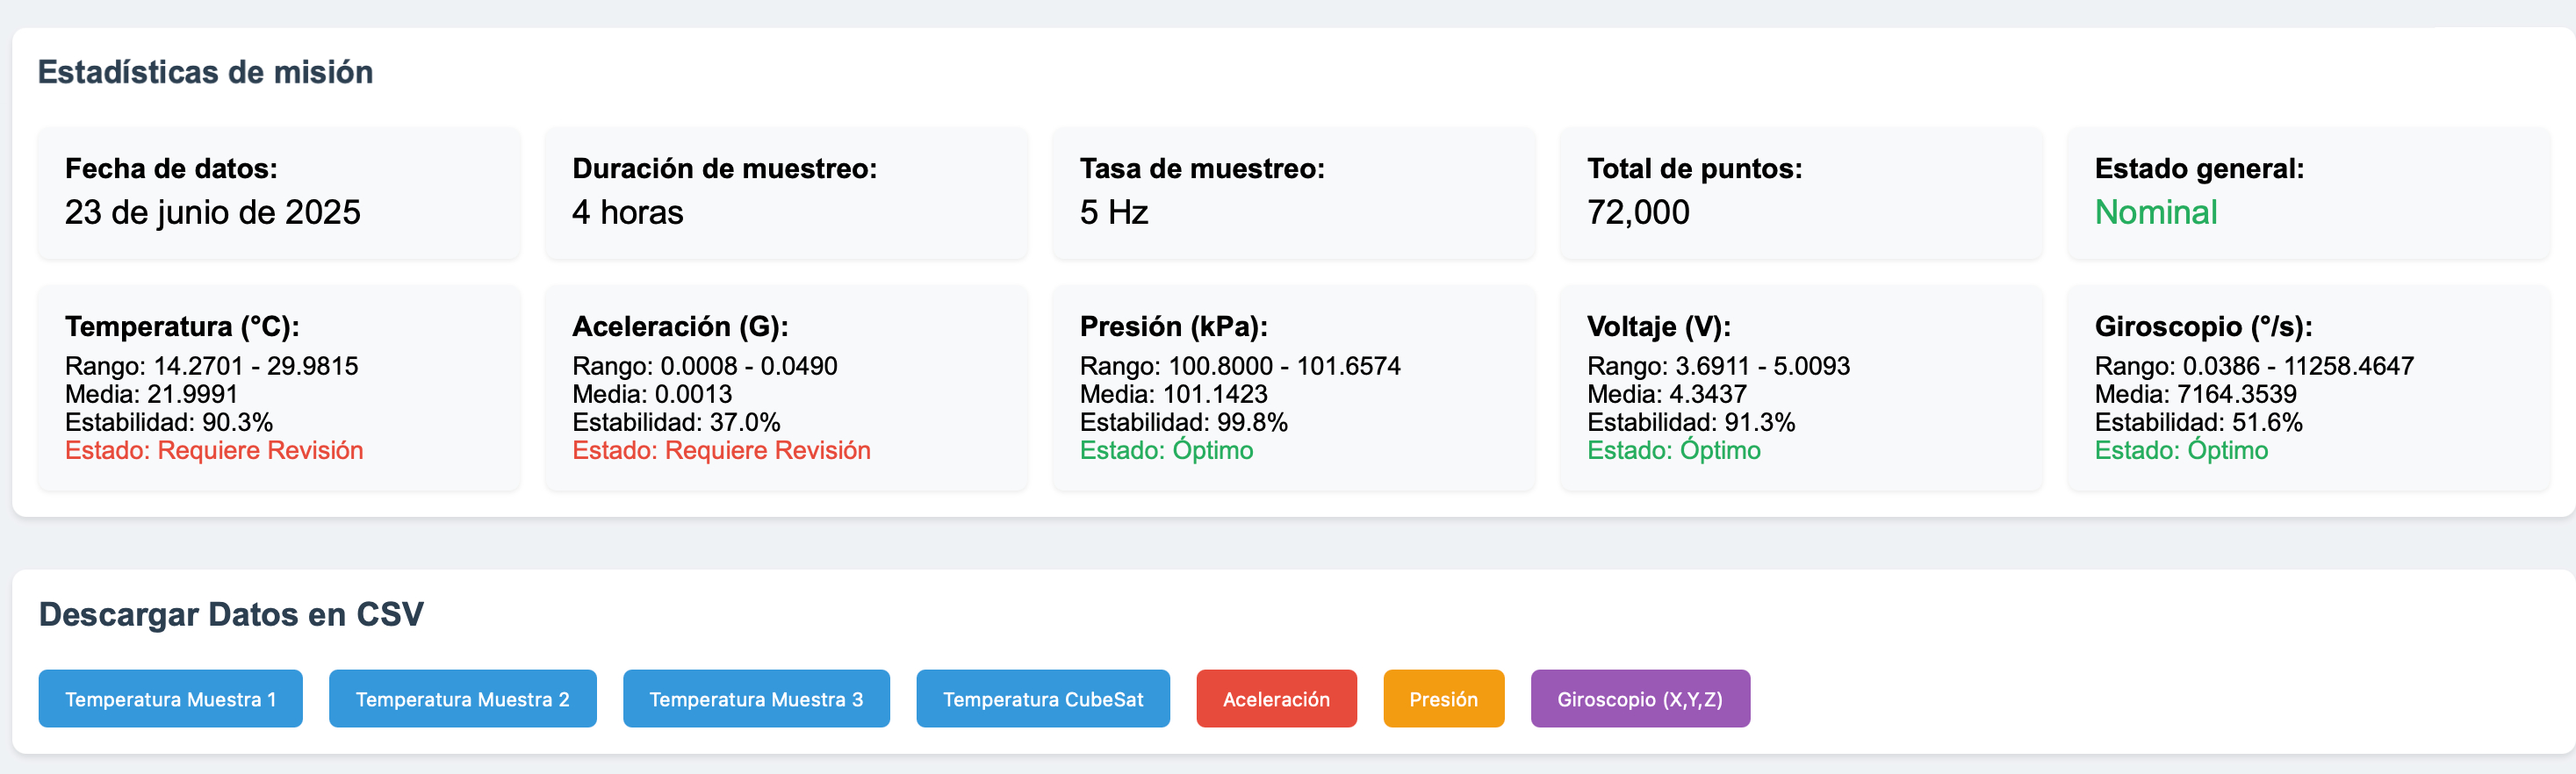
\includegraphics[width=18cm]{image/web/estadisticas.jpg}
    \caption{Página Web 2}
  \end{figure}
  \begin{figure}[H]
    \centering
    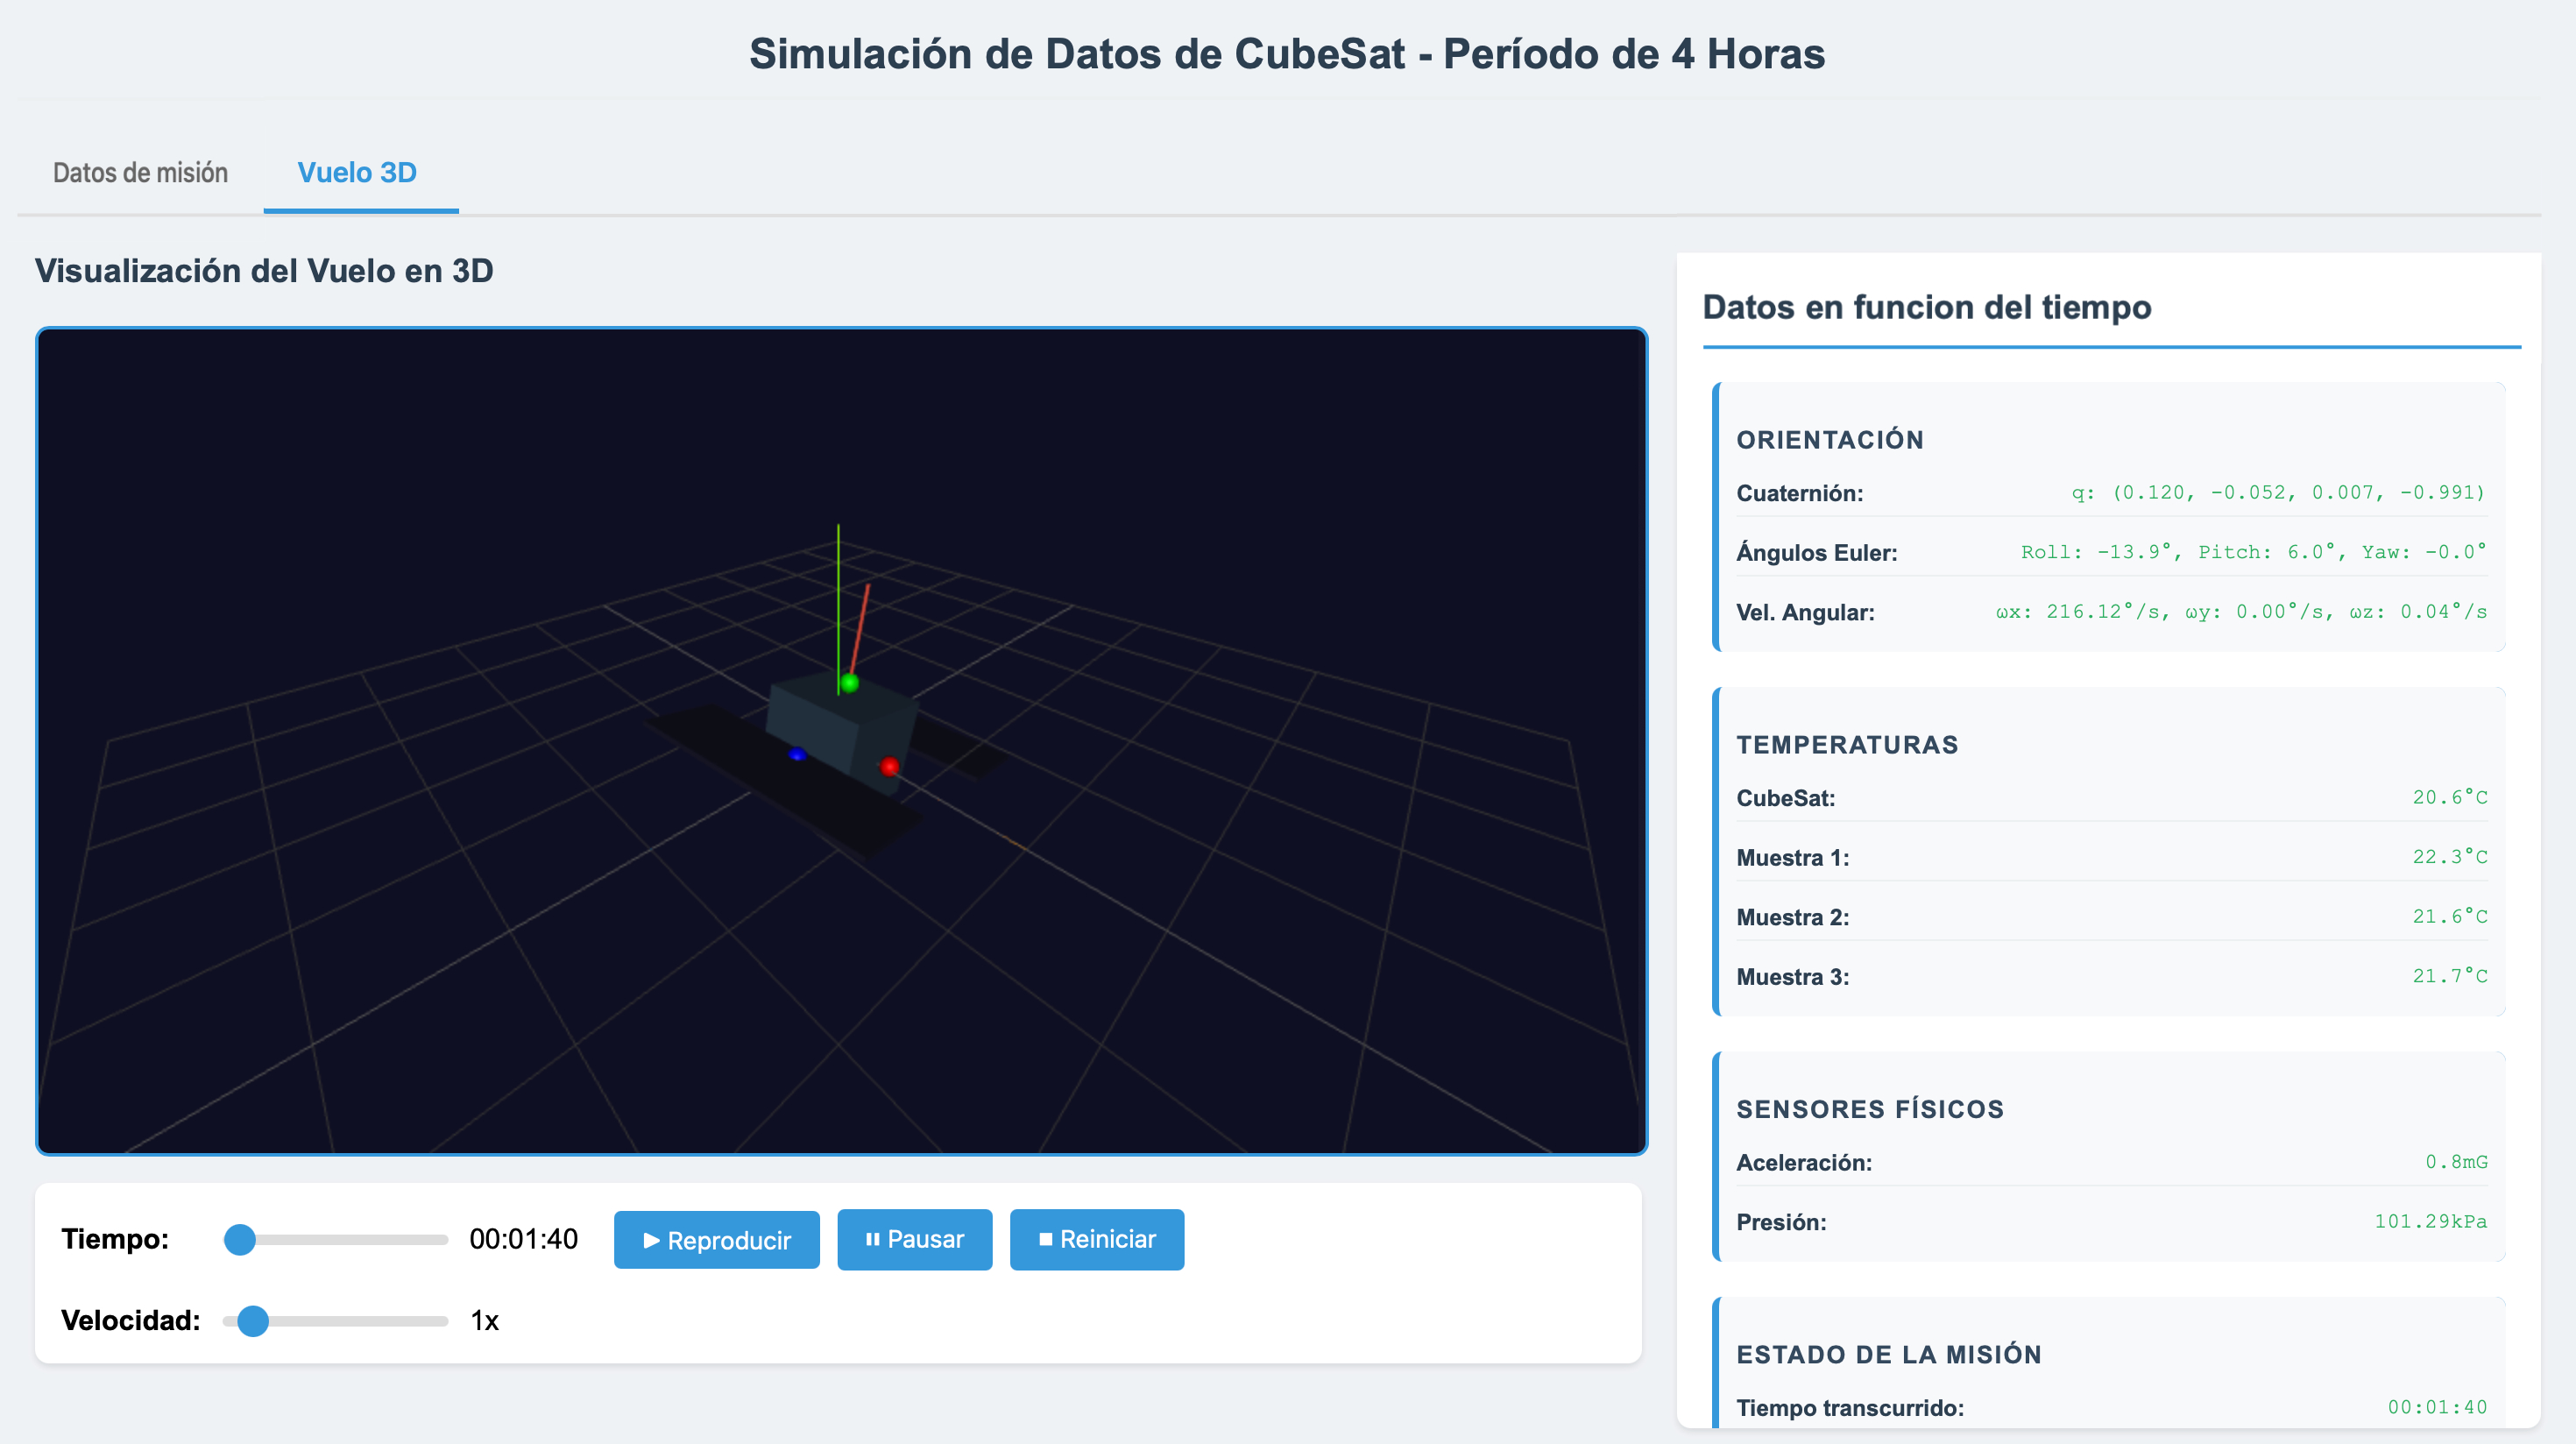
\includegraphics[width=18cm]{image/web/vuelo.jpg}
    \caption{Página Web 3}
  \end{figure}

\section{Simulaciones} \label{anexo:simulaciones}

  \begin{figure}[H]
    \centering
    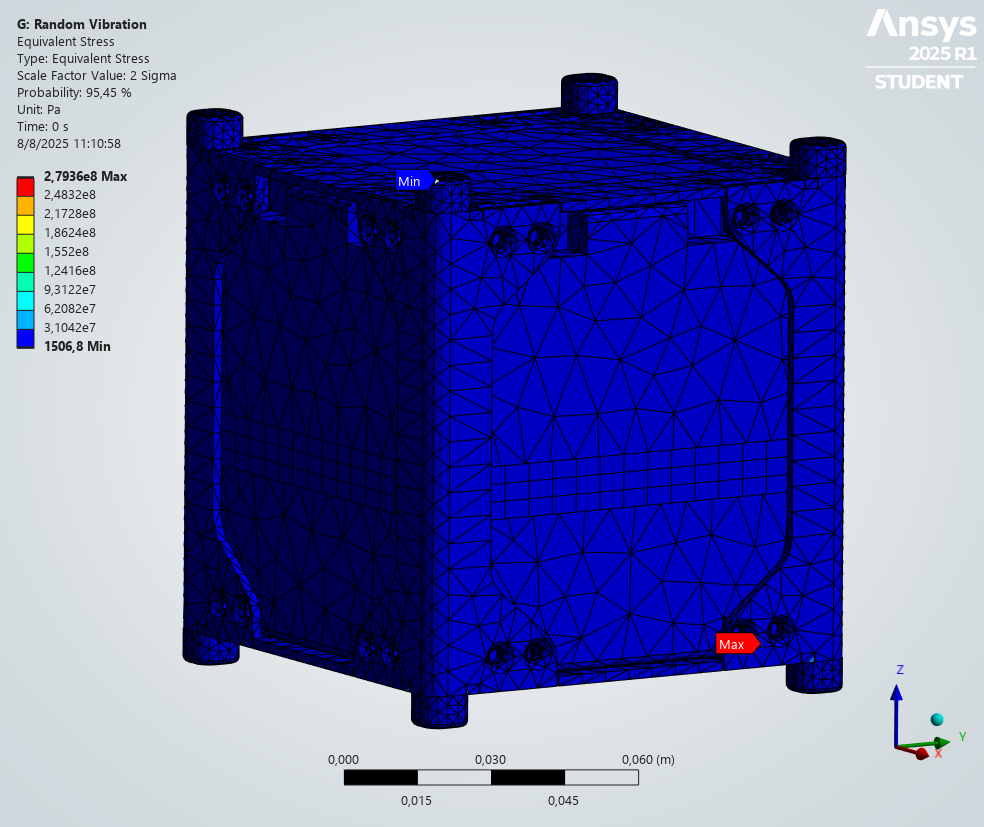
\includegraphics[width=15cm]{image/fem/ansys_cubesat-vibration_stress.png}
    \caption{Análisis de estrés}
  \end{figure}

  \begin{figure}[H]
    \centering
    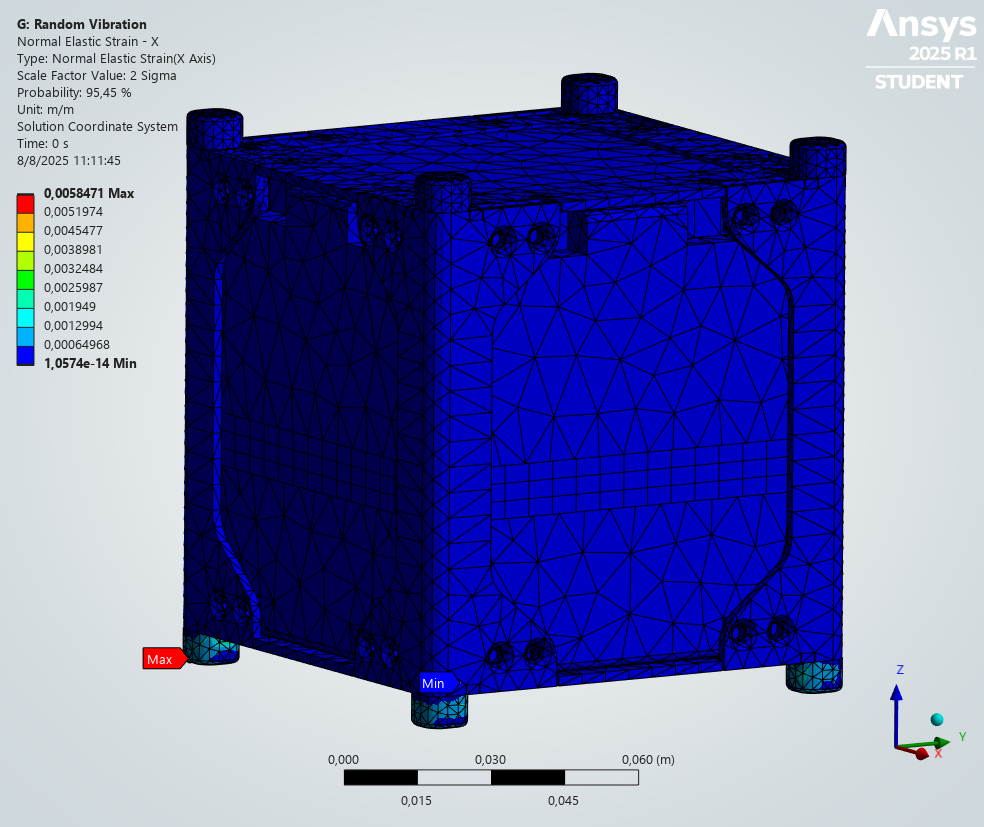
\includegraphics[width=14cm]{image/fem/ansys_cubesat-vibration_strain-x.png}
    \caption{Análisis de tensión en el eje x}
  \end{figure}

  \begin{figure}[H]
    \centering
    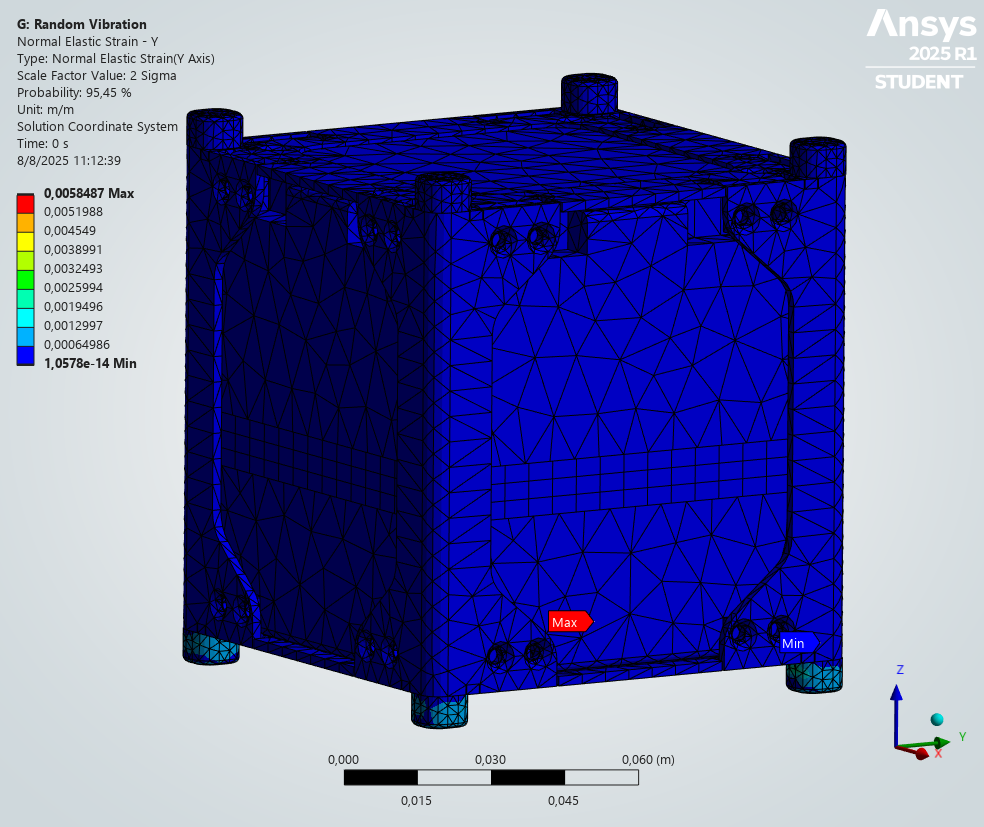
\includegraphics[width=14cm]{image/fem/ansys_cubesat-vibration_strain-y.png}
    \caption{Análisis de tensión en el eje Y}
  \end{figure}

  \begin{figure}[H]
    \centering
    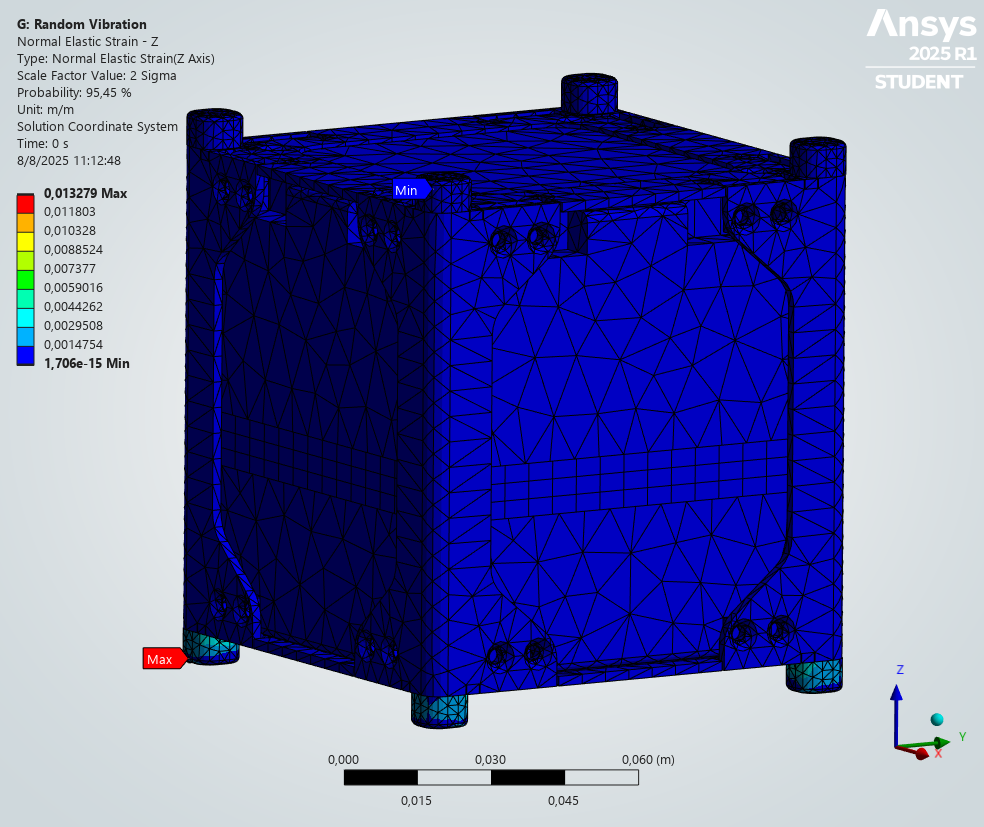
\includegraphics[width=14cm]{image/fem/ansys_cubesat-vibration_strain-z.png}
    \caption{Análisis de tensión en el eje Z}
  \end{figure}

  \begin{figure}[H]
    \centering
    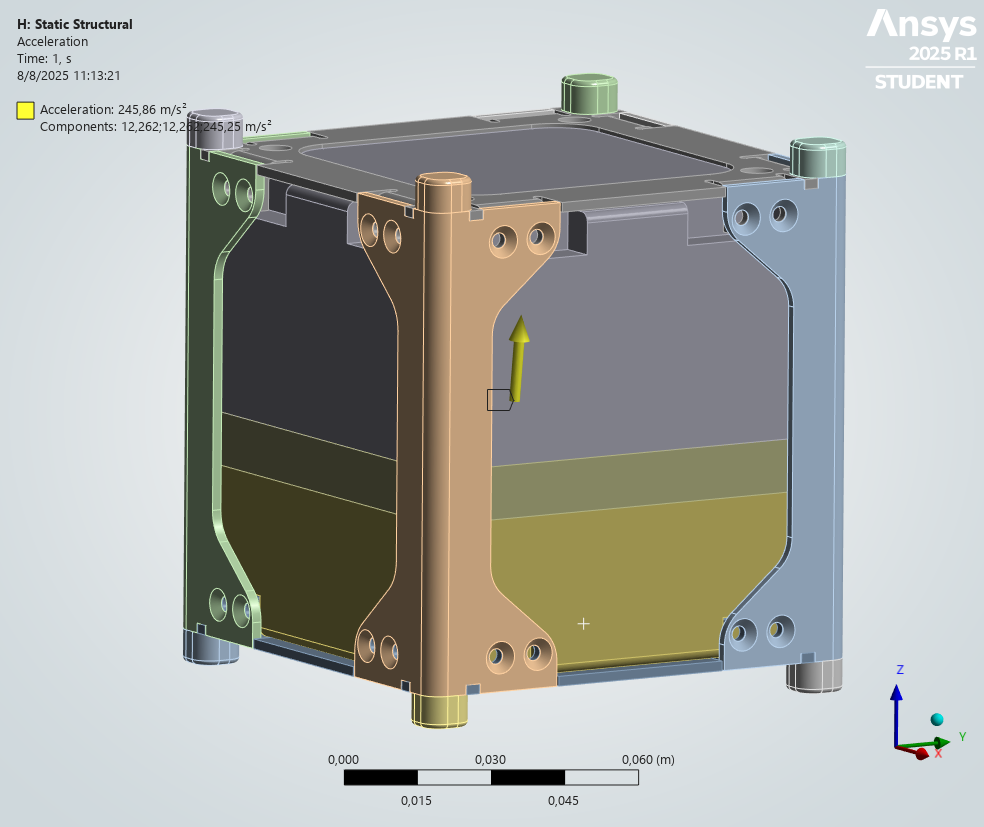
\includegraphics[width=14cm]{image/fem/ansys_cubesat-static_acceleration.png}
    \caption{Vector de aceleración para la simulación estática.}
  \end{figure}

  \begin{figure}[H]
    \centering
    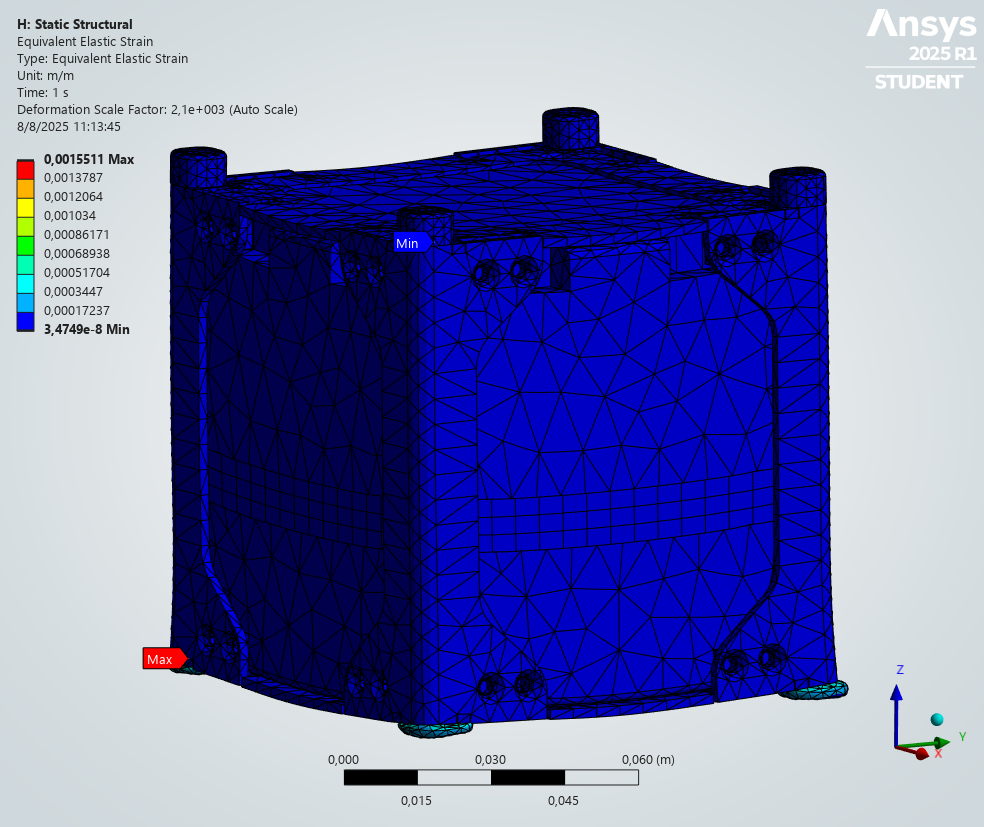
\includegraphics[width=14cm]{image/fem/ansys_cubesat-static_strain.png}
    \caption{Análisis de fatiga}
  \end{figure}

  \begin{figure}[H]
    \centering
    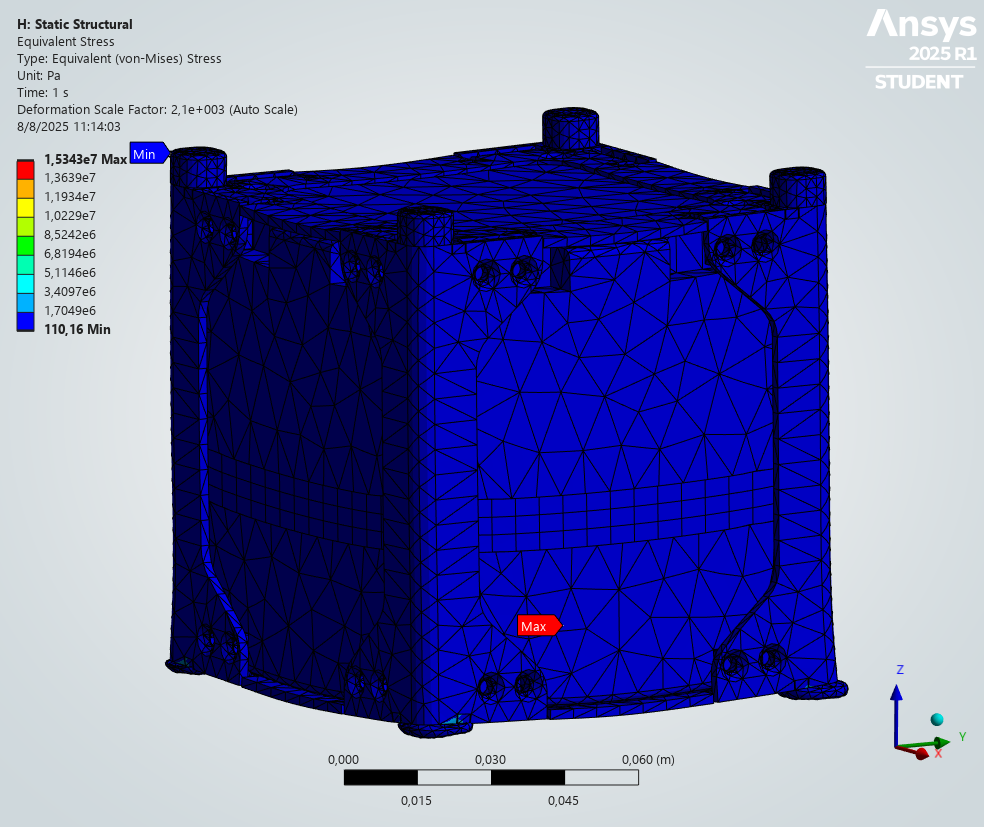
\includegraphics[width=14cm]{image/fem/ansys_cubesat-static_stress.png}
    \caption{Análisis de estrés}
  \end{figure}

  \begin{figure}[H]
    \centering
    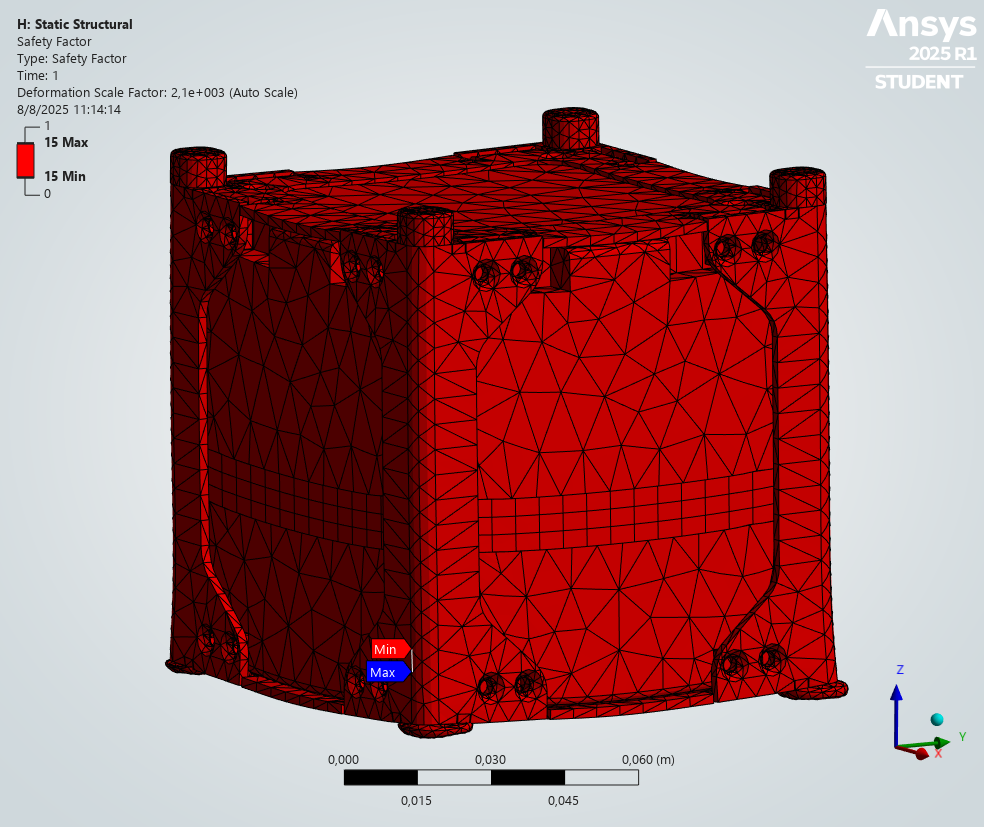
\includegraphics[width=14cm]{image/fem/ansys_cubesat-static_safety.png}
    \caption{Análisis de factor de seguridad}
  \end{figure}

  \begin{figure}[H]
    \centering
    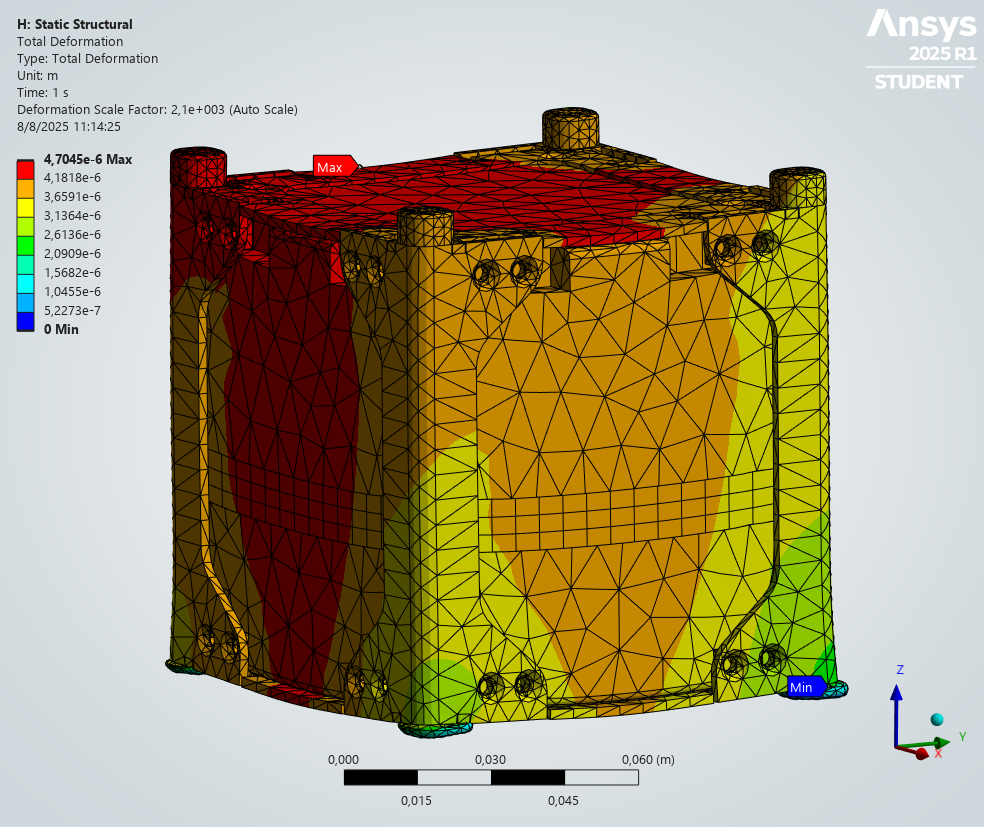
\includegraphics[width=14cm]{image/fem/ansys_cubesat-static_deformation.png}
    \caption{Análisis de deformación total}
  \end{figure}

\begin{landscape}
\section{Cronograma Mecánica}

 \begin{figure}[H]
  \centering
  \resizebox{25cm}{!}{%
  \begin{ganttchart}[
    hgrid,
    vgrid,
    time slot format=isodate,
    x unit=0.65cm,
    y unit chart=1cm,
    bar/.append style={fill=blue!40},
    milestone/.append style={fill=orange},
    milestone label font=\bfseries\small,
    bar label font=\small\slshape,
    group left shift=0,
    group right shift=0,
    group peaks tip position=0,
    group peaks height=.4
    ]{2025-07-04}{2025-08-22}

  % Tasks
  % Encabezado
  \gantttitlecalendar{month=name,week,day} \\

  \ganttgroup{Primer Prototipo (impreso en 3D)}{2025-07-04}{2025-07-09} \\
  \ganttbar{Impresión}{2025-07-04}{2025-07-06} \\
  \ganttbar{Integración}{2025-07-07}{2025-07-08} \\
  \ganttbar{Ensayos}{2025-07-08}{2025-07-09} \\

  \ganttgroup{Producto Mínimo}{2025-07-10}{2025-08-08} \\

  \ganttgroup{Segundo Prototipo (aluminio)}{2025-07-10}{2025-07-24} \\
  \ganttbar{Contacto Proveedores}{2025-07-10}{2025-07-14} \\
  \ganttbar{Correcciones de diseño}{2025-07-15}{2025-07-18} \\
  \ganttbar{Mecanizado}{2025-07-19}{2025-07-22} \\
  \ganttbar{Plegado}{2025-07-23}{2025-07-24} \\

  \ganttgroup{Desarrollo de Carcasas}{2025-07-10}{2025-07-24} \\
  \ganttbar{\acrshort{pms}}{2025-07-10}{2025-07-12} \\
  \ganttbar{\acrshort{obc}}{2025-07-13}{2025-07-15} \\
  \ganttbar{\acrshort{pu}}{2025-07-16}{2025-07-21} \\
  \ganttbar{Impresión 3D}{2025-07-21}{2025-07-24} \\

  \ganttbar{Integración General}{2025-07-25}{2025-07-30} \\
  \ganttbar{Ensayos}{2025-07-31}{2025-08-07} \\

  \ganttmilestone{Entrega \acrshort{cdr}}{2025-08-08} \\

  \ganttgroup{Producto Final}{2025-08-11}{2025-08-22} \\
  \ganttbar{Correcciones de diseño)}{2025-08-11}{2025-08-22} \\

  \end{ganttchart}
  }

  \caption{Cronograma equipo de mecánica, parte 1.}
     \label{gantt-mecanica1}
  \end{figure}

  \begin{figure}[H]
   \centering
   \resizebox{25cm}{!}{%
   \begin{ganttchart}[
     hgrid,
     vgrid,
     time slot format=isodate,
     x unit=0.65cm,
     y unit chart=1cm,
     bar/.append style={fill=blue!40},
     milestone/.append style={fill=orange},
     milestone label font=\bfseries\small,
     bar label font=\small\slshape,
     group left shift=0,
     group right shift=0,
     group peaks tip position=0,
     group peaks height=.4
     ]{2025-08-22}{2025-10-10}

   % Tasks
   % Encabezado
   \gantttitlecalendar{month=name,week,day} \\

  \ganttgroup{Producto Final}{2025-08-22}{2025-09-30} \\
   \ganttbar{Mecanizado}{2025-08-22}{2025-08-26} \\
   \ganttbar{Plegado}{2025-08-27}{2025-08-28} \\
   \ganttbar{Impresión 3D}{2025-08-22}{2025-08-22} \\
   \ganttbar{Integración (Modulos funcionales)}{2025-08-29}{2025-09-09} \\
   \ganttbar{Ensayos finales}{2025-09-10}{2025-09-30} \\

   % Milestone Informe final
   \ganttmilestone{Informe prelanzamiento}{2025-10-10}

   \end{ganttchart}
   }

  \caption{Cronograma equipo de mecánica, parte 2.}
      \label{gantt-mecanica2}
  \end{figure}

\section{Cronograma Electrónica (Hardware)}

 \begin{figure}[H]
  \centering
  \resizebox{25cm}{!}{%
  \begin{ganttchart}[
    hgrid,
    vgrid,
    time slot format=isodate,
    x unit=0.65cm,
    y unit chart=1cm,
    bar/.append style={fill=blue!40},
    milestone/.append style={fill=orange},
    milestone label font=\bfseries\small,
    bar label font=\small\slshape,
    group left shift=0,
    group right shift=0,
    group peaks tip position=0,
    group peaks height=.4
    ]{2025-07-04}{2025-08-31}

  % July
  \gantttitlecalendar{month=name,week,day} \\

  % Tasks
  \ganttgroup{Validación de Subsistemas}{2025-07-04}{2025-07-09} \\
  \ganttbar[name=rev-pcb]{Revisión de PCB}{2025-07-04}{2025-07-09} \\
  \ganttbar[name=rev-sensores]{Revisión de Sensores}{2025-07-04}{2025-07-09} \\

  \ganttgroup{CAD Computadora de Vuelo}{2025-07-10}{2025-07-17} \\
  \ganttbar[name=diseño-esq1]{Diseño esquemático}{2025-07-10}{2025-07-12} \\
  \ganttlinkedbar{Diseño PCB}{2025-07-13}{2025-07-16} \\
  \ganttlinkedmilestone[name=team-meating1]{Team Meeting}{2025-07-17} \\
  \ganttlink{rev-pcb}{diseño-esq1}
  \ganttlink[link mid=.25]{rev-sensores}{diseño-esq1}

  \ganttgroup{CAD PMS}{2025-07-18}{2025-07-24} \\
  \ganttbar[name=diseño-esq2]{Diseño esquemático}{2025-07-18}{2025-07-20} \\
  \ganttlinkedbar{Diseño PCB}{2025-07-20}{2025-07-23} \\
  \ganttlinkedmilestone[name=team-meating2]{Team Meeting}{2025-07-24} \\ 
  \ganttlink[link mid=.25]{team-meating1}{diseño-esq2}

  \ganttgroup{CAD TRU}{2025-07-25}{2025-07-31} \\
  \ganttbar[name=diseño-esq3]{Diseño esquemático}{2025-07-25}{2025-07-27} \\
  \ganttlinkedbar{Diseño PCB}{2025-07-27}{2025-07-30} \\
  \ganttlinkedmilestone{Team Meeting}{2025-07-31} \\
  \ganttlink[link mid=.25]{team-meating2}{diseño-esq3}

  \ganttlinkedbar{Prototipo Mínimo Funcional}{2025-08-01}{2025-08-07} \\
  \ganttlinkedmilestone[name=entrega-cdr]{Entrega \acrshort{cdr}}{2025-08-08} \\

  \ganttgroup{Construcción 1ra versión}{2025-08-09}{2025-08-18} \\
  \ganttbar[name=planchado]{Planchado de PCBs}{2025-08-09}{2025-08-11} \\
  \ganttlinkedbar{Soldado de componentes}{2025-08-12}{2025-08-12} \\
  \ganttlinkedbar[name=test-points]{Verificación de test points}{2025-08-13}{2025-08-14} \\
  \ganttlinkedbar{Interconexión de sistemas}{2025-08-15}{2025-08-18} \\
  \ganttbar[name=iden-errores]{Identificación de errores}{2025-08-15}{2025-08-18} \\
  \ganttlink[link mid=.25]{test-points}{iden-errores}  
  \ganttlink[link mid=.25]{entrega-cdr}{planchado}

  \ganttgroup{Construcción Producto Final}{2025-08-19}{2025-08-31} \\
  \ganttbar[name=planchado2]{Planchado de PCB}{2025-08-19}{2025-08-22} \\
  \ganttlink[link mid=.25]{iden-errores}{planchado2} 
  \ganttlinkedbar[name=soldado]{Soldado}{2025-08-23}{2025-08-24} \\
  \ganttlinkedbar[name=func-conj]{Funcionamiento en conjunto}{2025-08-24}{2025-08-31} \\
  \ganttbar[name=iden-fallas]{Identificación de posibles fallas}{2025-08-24}{2025-08-31} \\

  \ganttlink[link mid=.25]{soldado}{iden-fallas}
  \end{ganttchart}
  }

     \caption{Cronograma equipo de electrónica, desarrollo de hardware.}
     \label{gantt-hardware}
  \end{figure}


\section{Cronograma Electrónica (Firmware)}

 \begin{figure}[H]
  \centering
  \resizebox{25cm}{!}{%
  \begin{ganttchart}[
    hgrid,
    vgrid,
    time slot format=isodate,
    x unit=0.65cm,
    y unit chart=1cm,
    bar/.append style={fill=blue!40},
    milestone/.append style={fill=orange},
    milestone label font=\bfseries\small,
    bar label font=\small\slshape,
    group left shift=0,
    group right shift=0,
    group peaks tip position=0,
    group peaks height=.4
    ]{2025-08-09}{2025-10-10}

  % July
  \gantttitlecalendar{month=name,week=6,day} \\

  % Tasks
  \ganttgroup{Construcción 1ra versión}{2025-08-09}{2025-08-18} \\
  \ganttbar{Testing Subsistemas}{2025-08-15}{2025-08-18} \\

  \ganttgroup{Construcción Producto Final}{2025-08-19}{2025-08-31} \\
  \ganttbar[name=testing1]{Testing Subsistemas}{2025-08-25}{2025-08-31} \\

  \ganttgroup{Planificación de Firmware}{2025-09-01}{2025-09-08}\\
  \ganttbar[name=diagrama-flujo]{Diagrama de flujo}{2025-09-01}{2025-09-02} \\ 
  \ganttlinkedbar{Definición de Procesos}{2025-09-03}{2025-09-04} \\
  \ganttlinkedbar{Definición de Archivos}{2025-09-05}{2025-09-06} \\
  \ganttlinkedbar[name=def-funciones]{Definición de Funciones}{2025-09-07}{2025-09-08} \\
  \ganttlink[link mid=.25]{testing1}{diagrama-flujo}

  \ganttgroup{Desarrollo de Firmware}{2025-09-09}{2025-09-28}\\
  \ganttbar[name=prog-drivers]{Programación de Drivers}{2025-09-09}{2025-09-16} \\ 
  \ganttlinkedbar{Interrupciones y Manejo de Eventos}{2025-09-17}{2025-09-19} \\
  \ganttlinkedbar{Lógica integrada}{2025-09-20}{2025-09-25} \\
  \ganttlinkedbar{API de Datos}{2025-09-26}{2025-09-28} \\
  \ganttlinkedbar{Funcionamiento continuo}{2025-09-29}{2025-10-01}\\
  \ganttlinkedbar{Correción de errores}{2025-10-02}{2025-10-07}\\

  \ganttlink[link mid=.25]{def-funciones}{prog-drivers}

  \ganttmilestone{Informe prelanzamiento}{2025-10-10}

  \end{ganttchart}
  }
     \caption{Cronograma equipo de electrónica, desarrollo de firmware.}
    \label{gantt-firmware}
  \end{figure}

  \section{Cronograma Software}
    \begin{figure}[H]
      \centering
      \resizebox{25cm}{!}{%
        \begin{ganttchart}[
        hgrid,
        vgrid,
        time slot format=isodate,
        x unit=0.65cm,
        y unit chart=0.65cm,
        bar/.append style={fill=blue!40},
        milestone/.append style={fill=orange},
        milestone label font=\bfseries\small,
        bar label font=\small\slshape,
        group left shift=0,
        group right shift=0,
        group peaks tip position=0,
        group peaks height=.4
    ]{2025-07-04}{2025-08-17}

      \gantttitlecalendar{month=name, week, day} \\

      %\ganttlink{req}{tools}
      %\ganttlink{tools}{design}
      %\ganttlink{design}{developpdr}
      %\ganttlink{developpdr}{delivpdr}

      \ganttgroup{Desarrollo de \acrshort{cdr}}{2025-07-08}{2025-08-08} \\
      \ganttbar{Evaluación y revisión de correcciones}{2025-07-08}{2025-08-07} \\
      \ganttbar{Desarrollo de \acrshort{cdr}}{2025-07-08}{2025-08-07} \\
      \ganttlinkedmilestone[name=delivcdr]{Entrega de \acrshort{cdr}}{2025-08-08} \\

      \ganttgroup{Selección de equipo}{2025-08-09}{2025-08-14} \\
      \ganttbar{Evaluación}{2025-08-09}{2025-08-13} \\
      \ganttbar{Selección}{2025-08-14}{2025-08-14} \\

      \ganttgroup{Diseño de software}{2025-07-04}{2025-07-09} \\
      \ganttbar{Especificación de funcionalidades}{2025-07-04}{2025-07-09} \\
      \ganttbar{Diseño del sistema}{2025-07-04}{2025-07-09} \\

      \ganttgroup{Configuración de entorno}{2025-07-10}{2025-07-19} \\
      \ganttbar{Configuración del sistema operativo}{2025-07-10}{2025-07-14} \\
      \ganttbar{Instalación de herramientas}{2025-07-10}{2025-07-14} \\
      \ganttbar{Configuración de acceso}{2025-07-13}{2025-07-19} \\

      \ganttgroup{Integración de sensores}{2025-07-20}{2025-07-24} \\
      \ganttbar{Integración con lectura de sensores}{2025-07-20}{2025-07-22} \\
      \ganttbar{Compresión de datos}{2025-07-23}{2025-07-24} \\

      \ganttgroup{Sprint 1}{2025-07-25}{2025-08-17}\\

      \ganttgroup{Desarrollo backend}{2025-07-25}{2025-08-13} \\
      \ganttbar{Desarrollo de funcionalidades principales}{2025-07-25}{2025-07-31} \\
      \ganttbar{Análisis de datos}{2025-07-28}{2025-08-03} \\
      \ganttbar{Generación de reportes}{2025-08-04}{2025-08-08} \\
      \ganttbar{Manejo de errores}{2025-08-09}{2025-08-13} \\
      \ganttbar{Administración de logs}{2025-08-09}{2025-08-13} \\

      \ganttgroup{Almacenamiento}{2025-07-27}{2025-08-02} \\
      \ganttbar{Almacenamiento de datos}{2025-07-27}{2025-08-02} \\
      \ganttbar{Implementación RAID 1}{2025-07-27}{2025-08-02} \\

      \ganttgroup{Desarrollo frontend}{2025-08-04}{2025-08-10} \\
      \ganttbar{Interfaz visual}{2025-08-04}{2025-08-10} \\

      \ganttgroup{Testing}{2025-08-14}{2025-08-17} \\
      \ganttbar{Pruebas unitarias funcionales}{2025-08-14}{2025-08-15} \\
      \ganttbar{Pruebas unitarias no funcionales}{2025-08-14}{2025-08-15} \\
      \ganttbar{Pruebas de estrés}{2025-08-14}{2025-08-15} \\
      \ganttbar{Validación de hardware}{2025-08-16}{2025-08-17} \\
      \ganttbar{Corrección de posibles fallos}{2025-08-14}{2025-08-17} \\

    \end{ganttchart}
    }
    \caption{Cronograma equipo de software, parte 1.}
    \label{gantt-software1}
    \end{figure}

  \newpage
    \vspace*{\fill}
    \begin{figure}[H]
      \centering
      \resizebox{25cm}{!}{%
        \begin{ganttchart}[
        hgrid,
        vgrid,
        time slot format=isodate,
        x unit=0.65cm,
        y unit chart=0.65cm,
        bar/.append style={fill=blue!40},
        milestone/.append style={fill=orange},
        milestone label font=\bfseries\small,
        bar label font=\small\slshape,
        group left shift=0,
        group right shift=0,
        group peaks tip position=0,
        group peaks height=.4
    ]{2025-08-18}{2025-10-10}

      \gantttitlecalendar{month=name, week=8, day} \\

      %\ganttlink{req}{tools}
      %\ganttlink{tools}{design}
      %\ganttlink{design}{developpdr}
      %\ganttlink{developpdr}{delivpdr}

      \ganttgroup{Sprint 2}{2025-08-18}{2025-09-10}\\

      \ganttgroup{Desarrollo backend}{2025-08-18}{2025-09-06} \\
      \ganttbar{Desarrollo de funcionalidades principales}{2025-08-18}{2025-08-24} \\
      \ganttbar{Análisis de datos}{2025-08-21}{2025-08-27} \\
      \ganttbar{Generación de reportes}{2025-08-28}{2025-09-01} \\
      \ganttbar{Manejo de errores}{2025-09-02}{2025-09-06} \\
      \ganttbar{Administración de logs}{2025-09-02}{2025-09-06}\\

      \ganttgroup{Almacenamiento}{2025-08-20}{2025-08-26} \\
      \ganttbar{Almacenamiento de datos}{2025-08-20}{2025-08-26} \\
      \ganttbar{Implementación RAID 1}{2025-08-20}{2025-08-26}\\

      \ganttgroup{Desarrollo frontend}{2025-08-28}{2025-09-03} \\
      \ganttbar{Interfaz visual}{2025-08-28}{2025-09-03} \\

      \ganttgroup{Testing}{2025-09-07}{2025-09-10}  \\
      \ganttbar{Pruebas unitarias funcionales}{2025-09-07}{2025-09-08} \\
      \ganttbar{Pruebas unitarias no funcionales}{2025-09-07}{2025-09-08}  \\
      \ganttbar{Pruebas de estrés}{2025-09-07}{2025-09-08}  \\
      \ganttbar{Validación de hardware}{2025-09-09}{2025-09-10}  \\
      \ganttbar{Corrección de posibles fallos}{2025-09-07}{2025-09-10}  \\

      \ganttgroup{Sprint 3}{2025-09-11}{2025-10-04}\\

      \ganttgroup{Desarrollo backend}{2025-09-11}{2025-09-20} \\
      \ganttbar{Desarrollo de funcionalidades principales}{2025-09-11}{2025-09-17} \\
      \ganttbar{Análisis de datos}{2025-09-14}{2025-09-20} \\
      \ganttbar{Generación de reportes}{2025-09-21}{2025-09-25} \\
      \ganttbar{Manejo de errores}{2025-09-26}{2025-09-30} \\
      \ganttbar{Administración de logs}{2025-09-26}{2025-09-30} \\

      \ganttgroup{Almacenamiento}{2025-09-13}{2025-09-19} \\
      \ganttbar{Almacenamiento de datos}{2025-09-13}{2025-09-19} \\
      \ganttbar{Implementación RAID 1}{2025-09-13}{2025-09-19} \\

      \ganttgroup{Desarrollo frontend}{2025-09-21}{2025-09-27} \\
      \ganttbar{Interfaz visual}{2025-09-21}{2025-09-27} \\

      \ganttgroup{Testing}{2025-10-01}{2025-10-04} \\
      \ganttbar{Pruebas unitarias funcionales}{2025-10-01}{2025-10-02} \\
      \ganttbar{Pruebas unitarias no funcionales}{2025-10-01}{2025-10-02} \\
      \ganttbar{Pruebas de estrés}{2025-10-01}{2025-10-02} \\
      \ganttbar{Validación de hardware}{2025-10-03}{2025-10-04} \\
      \ganttbar{Corrección de posibles fallos}{2025-10-01}{2025-10-04} \\

      \ganttlinkedmilestone[name=delivcdr]{Entrega final}{2025-10-10}

      \end{ganttchart}
      }
    \caption{Cronograma equipo de software, parte 2.}
    \label{gantt-software2}
    \end{figure}
    \vspace*{\fill}
    \newpage
  
  \phantomsection
  \refstepcounter{section}
  \addcontentsline{toc}{section}{\numberline{\thesection}Esquematicos}
    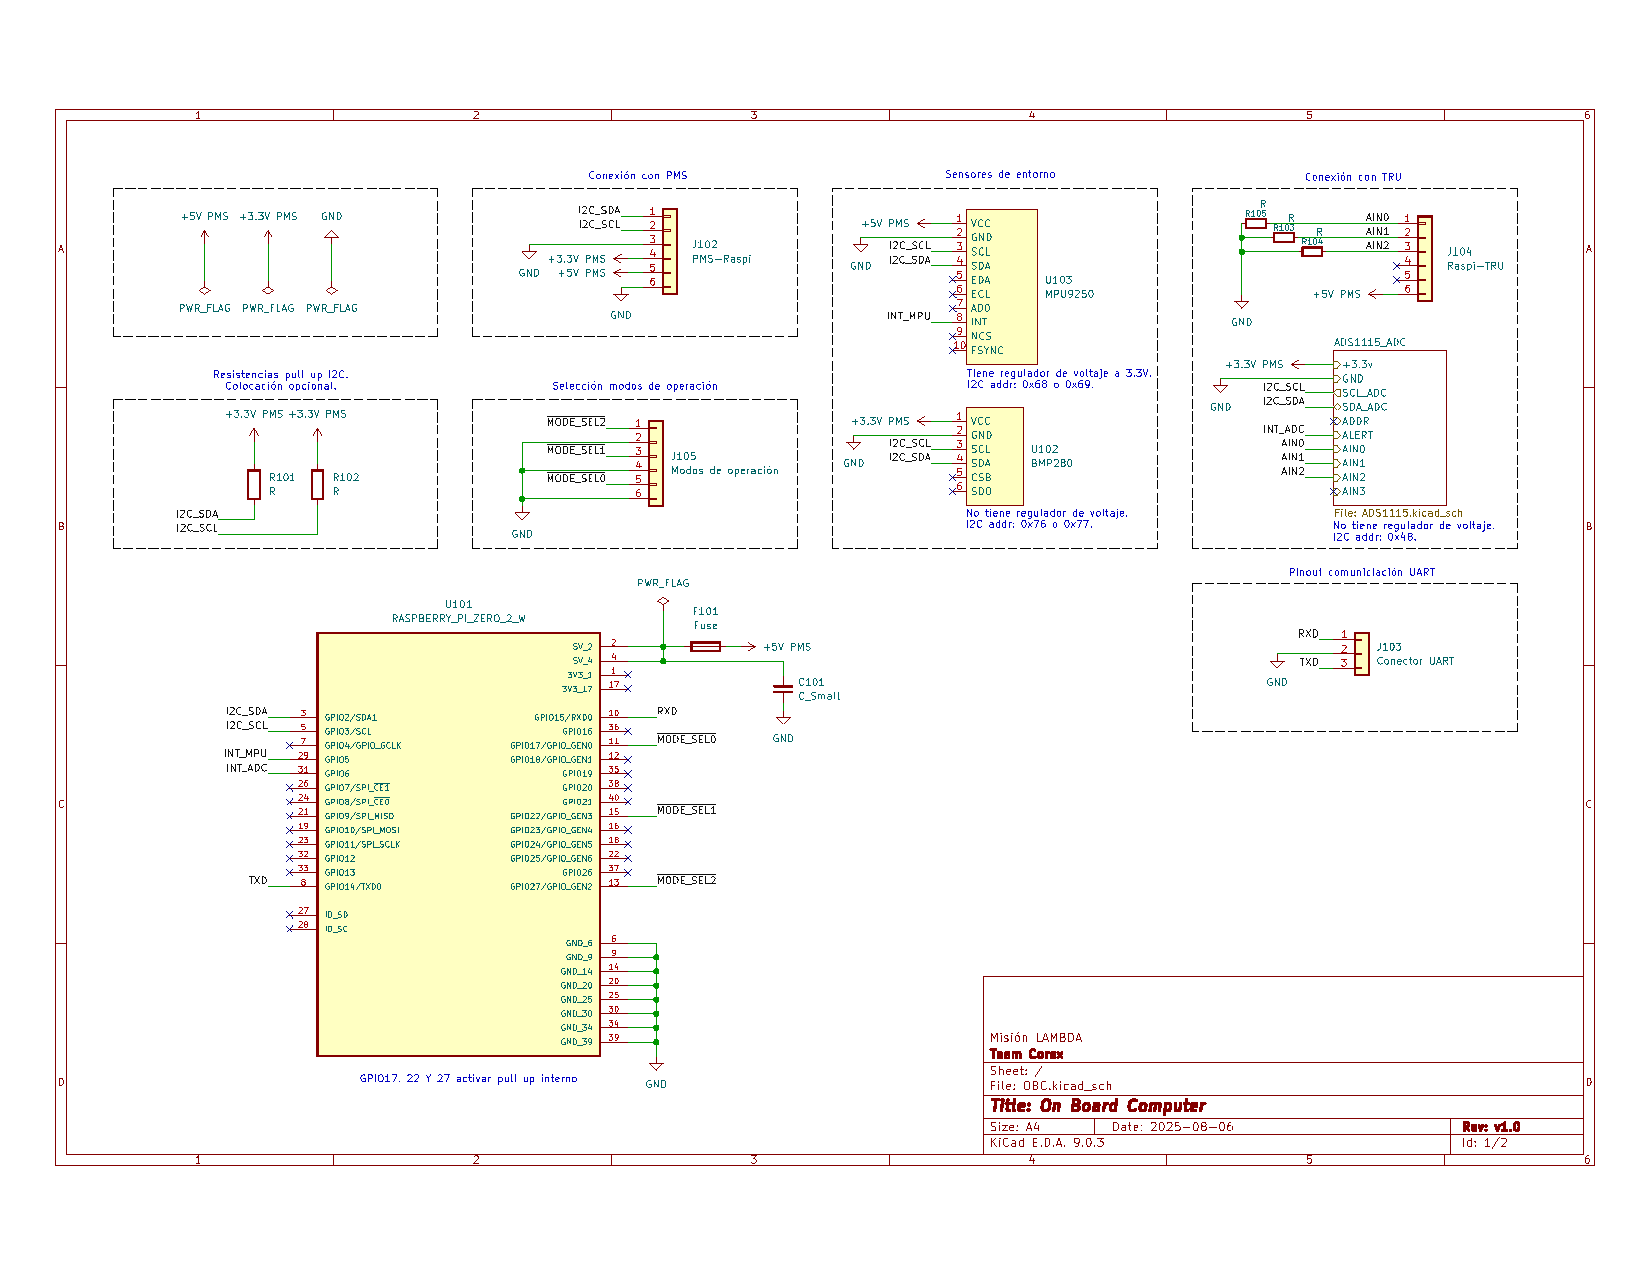
\includepdf[
      pages=-,
      pagecommand={\thispagestyle{plain}},
      addtotoc={1,subsection,1,{\acrfull{obc}},anexo:obc.schematic},
      landscape=true
    ]{annex/OBC_sch.pdf}
    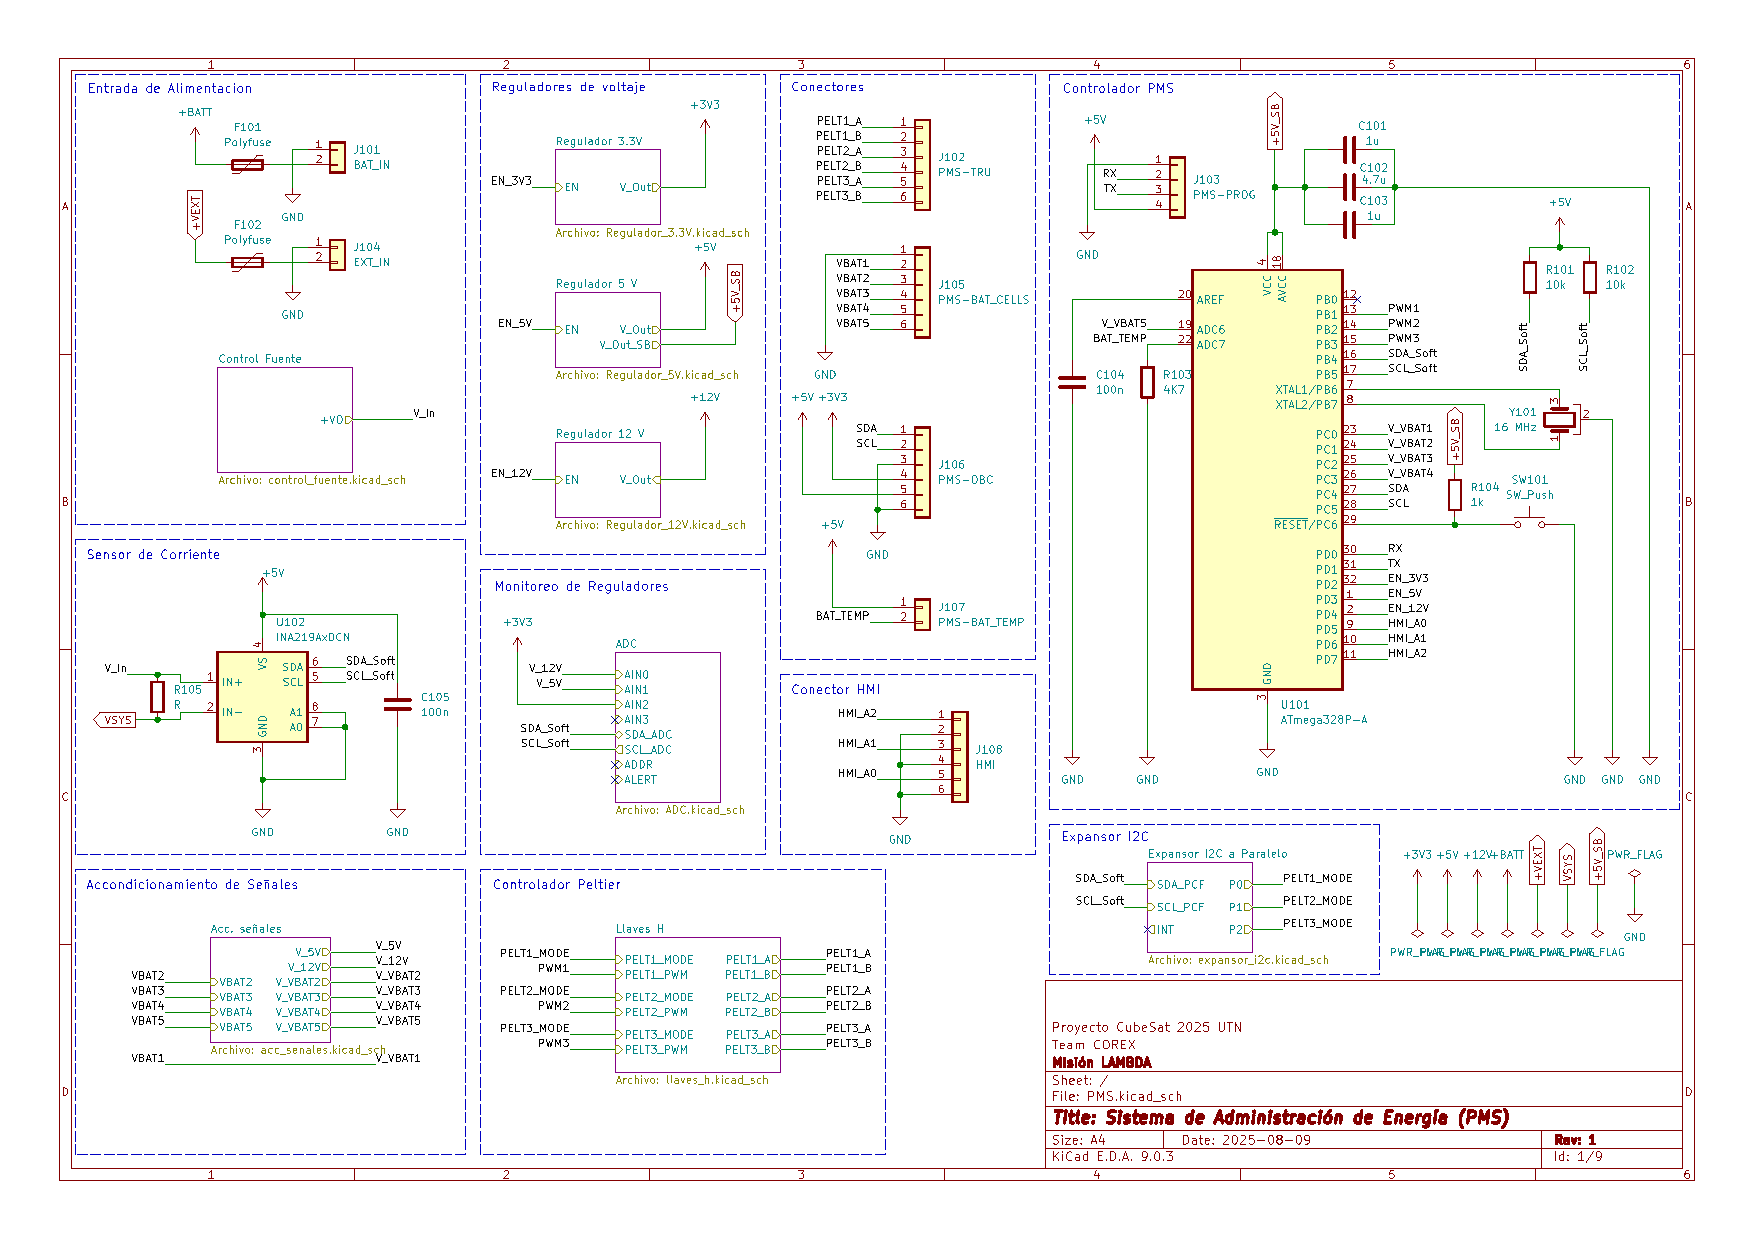
\includepdf[
      pages=-,
      pagecommand={\thispagestyle{plain}},
      addtotoc={1,subsection,1,{\acrfull{pms}},anexo:pms.schematic},
      landscape=true
    ]{annex/PMS_sch.pdf}

\end{landscape}
\restoregeometry
\setCustomPageStyle



\printbibliography[heading=bibnumbered]

\end{document}
